\documentclass[12pt]{article}
\usepackage{latex/ntgclass/a4}
\usepackage{epsfig}
%\usepackage{graphicx}
%\usepackage{floatfig}
%\usepackage{floatflt}
\usepackage{latex/subfigure/subfigure}
\usepackage{latex/multirow/multirow}
%\usepackage{rotate}
%\usepackage{rotating}
%\usepackage{doublespace}
\usepackage{latex/setspace/setspace}

\include{latex/header}

\usepackage{lmodern}
\renewcommand\ttfamily{\usefont{T1}{lmtt}{m}{n}}

\newcommand{\TT}[1]{{\ttfamily\bfseries #1}}
\newcommand{\Tt}[1]{{\tt #1}}
\newcommand{\NAME}{{\TT{SimGen}}}

\setstretch{1.5}

\begin{document}

\title{\bf \NAME --- a generalised multi-scale modelling and simulation program
}

\author{
William~R.~Taylor\\ \\ \\ \\
$^\dagger$Division of Mathematical Biology,\\
MRC National Institute for Medical Research,\\
The Ridgeway, Mill Hill, London NW7 1AA, U.K.\\ \\ 
}
\begin{singlespace}
\maketitle
\end{singlespace}
\clearpage
%\include{abstract}
%\clearpage
\part{Overview and Model Design}
% Organizing document for the Infernal User's Guide
%
% SVN $Id: main.tex 4240 2012-10-11 16:24:35Z nawrockie $

\documentclass[10pt]{article}
%\usepackage{helvetic}
\usepackage{times}
\usepackage{fullpage}
\usepackage{fancybox}  % Must include fancybox *before* fancyvrb;
\usepackage{fancyvrb}  % don't know why.
\usepackage[pdftex]{graphicx}
\usepackage{url}
%\usepackage[backref,colorlinks]{hyperref}
\usepackage[authoryear]{natbib}

\usepackage{verbatim}

\setcounter{secnumdepth}{1}
\renewcommand{\familydefault}{\sfdefault}
% Typography.
\newcommand{\ccode}[1]{{\smaller\texttt{#1}}}
\newcommand{\emcode}[1]{{\smaller\texttt{\textbf{#1}}}}
\newcommand{\itcode}[1]{{\smaller\texttt{\textit{#1}}}}
\newcommand{\itbfcode}[1]{{\smaller\texttt{\textit{\bfseries #1}}}}
\newcommand{\esldef}[1]{\textbf{#1}}                    % Define/introduce a term (to be indexed)
\newcommand{\prog}[1]{{\smaller\textsc{#1}}}
\newcommand{\eslmod}[1]{{\smaller\textsf{\textup{\textbf{#1}}}}}
\newcommand{\user}[1]{\indent\indent{\small\bfseries\texttt{> #1}}}
\newcommand{\response}[1]{\indent\indent{\small\texttt{#1}}}

\newcommand{\Easel}   {{\smaller\textsc{easel}}}
\newcommand{\HMMER}   {{\smaller\textsc{hmmer}}}
\newcommand{\Infernal}{{\smaller\textsc{infernal}}}
\newcommand{\Pfam}    {{\smaller\textsc{pfam}}}
\newcommand{\Rfam}    {{\smaller\textsc{rfam}}}

% \api* functions are for the API summary tables.
\newcommand{\apisubhead}[1]{\multicolumn{2}{|c|}{\rule[-0.4em]{0em}{1.5em}\textbf{#1}}}

\def\argmax{\mathop{\mathrm{argmax}}\limits}
\def\argmin{\mathop{\mathrm{argmin}}\limits}

\DefineVerbatimEnvironment{cchunk}{Verbatim}{numbers=right,fontsize=\scriptsize,xleftmargin=1.0\parindent}%
\DefineVerbatimEnvironment{userchunk}{Verbatim}{fontseries=b,fontsize=\small,xleftmargin=1.0\parindent}%
\DefineVerbatimEnvironment{responsechunk}{Verbatim}{fontsize=\small,xleftmargin=1.0\parindent}%


% Description-like environment for documenting functions/APIs.
% puts the description label in a minipage with a large hanging
% indent.
% Good christ this took a long time to develop.
% hanging indent trick stolen from Peter Wilson's hanging.sty @CTAN
% minipage allows multi-line label, and puts item on next line.
% customized list inspired by Kopka/Daly _Guide to LaTeX_ p.213
% SRE, Wed Dec 27 11:37:18 2000
%
\newenvironment{sreapi}{%
     \begin{list}{}{%
       \renewcommand{\makelabel}[1]{%
         \begin{minipage}{\textwidth}%
           \hangindent10em\hangafter1\noindent%
           {\bfseries\texttt{##1}\vspace{0.8em}}%
         \end{minipage}%
     }}}%
     {\end{list}}


% Description-like environment for producing lists like:
%
%     label  stuff, stuff, stuff
%
%    label2  more stuff, more stuff,
%            more stuff.
% \begin{sreitems}{Longest label} \item[label] stuff, ... \end{sreitems}
% SRE, Wed Dec 27 11:59:43 2000
%
\newenvironment{sreitems}[1]{%
     \begin{list}{}{%
       \settowidth{\labelwidth}{#1}%
       \setlength{\leftmargin}{\labelwidth}%
       \addtolength{\leftmargin}{\labelsep}%
       }}
     {\end{list}}


\begin{document}

\bibliographystyle{apalike}

\begin{titlepage}
{\Large

\vspace*{\fill}

\noindent
{\Huge{Easel}} \\ 
\rule[2pt]{\textwidth}{1pt} \\
\hspace*{\fill} {\large {A library of C functions for
    biological sequence analysis} \\ }

\vspace*{\fill}

\begin{center}
\url{http://selab.janelia.org/easel/}\\
Version 0.1; March 2008 \\ 

\vspace*{\fill}

Sean R. Eddy\\
HHMI Janelia Farm Research Campus\\
19700 Helix Drive\\
Ashburn VA 20147\\
\url{http://selab.janelia.org/}\\
\end{center}

\vspace*{\fill}
}
\end{titlepage}

\vspace*{\fill}
\begin{flushleft}
Copyright (C) 2008 Howard Hughes Medical Institute.

\vspace{2em} 

Easel's source code and documentation are freely redistributable and
modifiable under the terms of the Janelia Farm Software License.
\end{flushleft}









\newpage
\tableofcontents

\newpage
\section{Introduction}
\setcounter{footnote}{0}

HMMER is used to search sequence databases for homologs of protein
sequences, and to make protein sequence alignments. HMMER can be used
to search sequence databases with single query sequences but it
becomes particularly powerful when the query is an multiple sequence
alignment of a sequence family. HMMER makes a \emph{profile} of the
query that assigns a position-specific scoring system for
substitutions, insertions, and deletions. HMMER profiles are
probabilistic models called ``profile hidden Markov models'' (profile
HMMs) \citep{Krogh94,Eddy98,Durbin98}.

Compared to BLAST, FASTA, and other sequence alignment and database
search tools based on older scoring methodology, HMMER aims to be
significantly more accurate and more able to detect remote homologs,
because of the strength of its underlying probability models. In the
past, this strength came at a significant computational cost, with
profile HMM implementations running about 100x slower than comparable
BLAST searches. With HMMER3, HMMER is now essentially as fast as
BLAST.


\subsection{How to avoid reading this manual}

I hate reading documentation. If you're like me, you're sitting here
thinking, \pageref{manualend} pages of documentation, you must be
joking! I just want to know that the software compiles, runs, and
gives apparently useful results, before I read some 
\pageref{manualend} exhausting pages of someone's documentation. For
cynics that have seen one too many software packages that don't
work:

\begin{itemize}
\item Follow the quick installation instructions on page
      \pageref{section:installation}. An automated test suite
      is included, so you will know immediately if something
      went wrong.\footnote{Nothing should go wrong.}
\item Go to the tutorial section on page
\pageref{section:tutorial}, which walks you through some examples of
using HMMER on real data.
\end{itemize}

Everything else, you can come back and read later.



\subsection{How to avoid using this software (links to similar software)}

Several implementations of profile HMM methods and related
position-specific scoring matrix methods are available. 

\begin{center}
\begin{tabular}{lp{5in}l}
Software  &   URL \\ \hline
HMMER     & \url{http://hmmer.org/}\\
SAM       & \url{http://www.cse.ucsc.edu/research/compbio/sam.html}\\
PSI-BLAST & \url{http://www.ncbi.nlm.nih.gov/Education/BLASTinfo/psi1.htm}\\
PFTOOLS   & \url{http://www.isrec.isb-sib.ch/profile/profile.html}\\
\end{tabular}
\end{center}

The UC Santa Cruz SAM software is the closest relative of HMMER.


\subsection{What profile HMMs are}

Profile HMMs are statistical models of multiple sequence alignments,
or even of single sequences. They capture position-specific
information about how conserved each column of the alignment is, and
which residues are likely.  Anders Krogh, David Haussler, and
co-workers at UC Santa Cruz introduced profile HMMs to computational
biology \citep{Krogh94}, adopting HMM techniques which have been used
for years in speech recognition. HMMs had been used in biology before
the Krogh/Haussler work, notably by Gary Churchill \citep{Churchill89},
but the Krogh paper had a dramatic impact because HMM technology was
so well-suited to the popular ``profile'' methods for searching
databases using multiple sequence alignments instead of single query
sequences.

``Profiles'' had been introduced by Gribskov and colleagues
\citep{Gribskov87,Gribskov90}, and several other groups introduced
similar approaches at about the same time, such as ``flexible
patterns'' \citep{Barton90}, and
``templates''\citep{Bashford87,Taylor86}. The term ``profile'' has
stuck.\footnote{There has been agitation in some quarters to call all
  such models ``position specific scoring matrices'', PSSMs, but
  certain small nocturnal North American marsupials have a prior claim
  on the name.}  All profile methods (including PSI-BLAST
\citep{Altschul97}) are more or less statistical descriptions of the
consensus of a multiple sequence alignment. They use
\emph{position-specific} scores for amino acids (or nucleotides) and
position specific penalties for opening and extending an insertion or
deletion.  Traditional pairwise alignment (for example, BLAST
\citep{Altschul90}, FASTA \citep{Pearson88}, or the Smith/Waterman
algorithm \citep{Smith81}) uses position-{\em independent} scoring
parameters. This property of profiles captures important information
about the degree of conservation at various positions in the multiple
alignment, and the varying degree to which gaps and insertions are
permitted.

The advantage of using HMMs is that HMMs have a formal probabilistic
basis. We use probability theory to guide how all the scoring
parameters should be set. Though this might sound like a purely
academic issue, this probabilistic basis lets us do things that more
heuristic methods cannot do easily. One of the most important is that
HMMs have a consistent theory for setting position-specific gap and
insertion scores. The methods are consistent and therefore highly
automatable, allowing us to make libraries of hundreds of profile HMMs
and apply them on a very large scale to whole genome analysis.  One
such database of protein domain models is Pfam
\citep{Sonnhammer97,Finn10}, which is a significant part of the
Interpro protein domain annotation system \citep{Mulder03}. The
construction and use of Pfam is tightly tied to the HMMER software
package.

Profile HMMs do have important limitations. One is that HMMs do not
capture any higher-order correlations.  An HMM assumes that the
identity of a particular position is independent of the identity of
all other positions.\footnote{This is not strictly true. There is a
  subtle difference between an HMM's state path (a first order Markov
  chain) and the sequence described by an HMM (generated from the
  state path by independent emissions of symbols at each state).}
Profile HMMs are often not good models of structural RNAs, for
instance, because an HMM cannot describe base pairs.



\subsection{Applications of profile HMMs}

HMMER can be used to replace BLASTP and PSI-BLAST for searching
databases with single query sequences. With HMMER3, we now include two
programs for searching databases with single query sequences:
\prog{phmmer} and \prog{jackhmmer}, where \prog{jackhmmer} is an
iterative search akin to PSI-BLAST.

Another application of HMMER is when you are working on a protein
sequence family, and you have carefully constructed a multiple
sequence alignment. Your family, like most protein families, has a
number of strongly (but not absolutely) conserved key residues,
separated by characteristic spacing. You wonder if there are more
members of your family in the sequence databases, but the family is so
evolutionarily diverse, a BLAST search with any individual sequence
doesn't even find the rest of the sequences you already know
about. You're sure there are some distantly related sequences in the
noise. You spend many pleasant evenings scanning weak BLAST alignments
by eye to find ones with the right key residues are in the right
places, but you wish there was a computer program that did this a
little better.

Another application is the automated annotation of the domain
structure of proteins. Large databases of curated alignments and HMMER
models of known domains are available, including Pfam \citep{Finn10}
and SMART \citep{Letunic06} in the Interpro database consortium
\citep{Mulder03}. (Many ``top ten protein domains'' lists, a standard
table in genome analysis papers, rely heavily on HMMER annotation.)
Say you have a new sequence that, according to a BLAST analysis, shows
a slew of hits to receptor tyrosine kinases. Before you decide to call
your sequence an RTK homologue, you suspiciously recall that RTK's
are, like many proteins, composed of multiple functional domains, and
these domains are often found promiscuously in proteins with a wide
variety of functions. Is your sequence really an RTK? Or is it a novel
sequence that just happens to have a protein kinase catalytic domain
or fibronectin type III domain?

Another application is the automated construction and maintenance
of large multiple alignment databases.  It is useful to organize
sequences into evolutionarily related families. But there are
thousands of protein sequence families, some of which comprise tens of
thousands of sequences -- and the primary sequence databases continue
to double every year or two. This is a hopeless task for manual
curation; but on the other hand, manual curation is still necessary
for high-quality, biologically relevant multiple alignments. Databases
like Pfam \citep{Finn10} are constructed by distinguishing between a
stable curated ``seed'' alignment of a small number of representative
sequences, and ``full'' alignments of all detectable homologs; HMMER
is used to make a model of the seed, search the database for homologs,
and automatically produce the full alignment by aligning every
sequence to the seed consensus.

You may find other applications as well. Using hidden Markov models to
make a linear consensus model of a bunch of related strings is a
pretty generic problem, and not just in biological sequence analysis.
HMMER3 has already been used to model mouse song [Elena Rivas,
  personal communication] and in the past HMMER has reportedly been
used to model music, speech, and even automobile engine telemetry. If
you use it for something particularly strange, I'd be curious to hear
about it -- but I never, ever want to see my error messages showing up
on the console of my Saab.



\subsection{Design goals of HMMER3}

In the past, profile HMM methods were considered to be too
computationally expensive, and BLAST has remained the main workhorse
of sequence similarity searching. The main objective of the HMMER3
project (begun in 2004) is to combine the power of probabilistic
inference with high computational speed. We aim to upgrade some of
molecular biology's most important sequence analysis applications to
use more powerful statistical inference engines, without sacrificing
computational performance.

Specifically, HMMER3 has three main design features that \emph{in
combination} distinguish it from previous tools:

\begin{description}
\item[\textbf{Explicit representation of alignment uncertainty.}]
  Most sequence alignment analysis tools report only a single
  best-scoring alignment. However, sequence alignments are uncertain,
  and the more distantly related sequences are, the more uncertain
  alignments become. HMMER3 calculates complete posterior alignment
  ensembles rather than single optimal alignments. Posterior ensembles
  get used for a variety of useful inferences involving alignment
  uncertainty. For example, any HMMER3 sequence alignment is
  accompanied by posterior probability annotation, representing the
  degree of confidence in each individual aligned residue.

\item[\textbf{Sequence scores, not alignment scores.}]  Alignment
  uncertainty has an important impact on the power of sequence
  database searches.  It's precisely the most remote homologs -- the
  most difficult to identify and potentially most interesting
  sequences -- where alignment uncertainty is greatest, and where the
  statistical approximation inherent in scoring just a single best
  alignment breaks down the most. To maximize power to discriminate
  true homologs from nonhomologs in a database search, statistical
  inference theory says you ought to be scoring sequences by
  integrating over alignment uncertainty, not just scoring the single
  best alignment. HMMER3's log-odds scores are sequence scores, not
  just optimal alignment scores; they are integrated over the
  posterior alignment ensemble.
  
\item[\textbf{Speed.}] A major limitation of previous profile HMM
  implementations (including HMMER2) was their slow
  performance. HMMER3 implements a new heuristic acceleration
  algorithm. For most queries, it's about as fast as BLAST.
\end{description}

Individually, none of these points is new. As far as alignment
ensembles and sequence scores go, pretty much the whole reason why
hidden Markov models are so theoretically attractive for sequence
analysis is that they are good probabilistic models for explicitly
dealing with alignment uncertainty. The SAM profile HMM software from
UC Santa Cruz has always used full probabilistic inference (the HMM
Forward and Backward algorithms) as opposed to optimal alignment
scores (the HMM Viterbi algorithm). HMMER2 had the full HMM inference
algorithms available as command-line options, but used Viterbi
alignment by default, in part for speed reasons. Calculating alignment
ensembles is even more computationally intensive than calculating
single optimal alignments.

One reason why it's been hard to deploy sequence scores for practical
large-scale use is that we haven't known how to accurately calculate
the statistical significance of a log-odds score that's been
integrated over alignment uncertainty. Accurate statistical
significance estimates are essential when one is trying to
discriminate homologs from millions of unrelated sequences in a large
sequence database search. The statistical significance of optimal
alignment scores can be calculated by Karlin/Altschul statistics
\citep{Karlin90,KarlinAltschul93}. Karlin/Altschul statistics are one
of the most important and fundamental advances introduced by BLAST.
However, this theory doesn't apply to integrated log-odds sequence
scores (HMM ``Forward scores'').  The statistical significance
(expectation values, or E-values) of HMMER3 sequence scores is
determined by using recent theoretical conjectures about the
statistical properties of integrated log-odds scores which have been
supported by numerical simulation experiments \citep{Eddy08}.

And as far as speed goes, there's really nothing new about HMMER3's
speed either. Besides Karlin/Altschul statistics, the main reason
BLAST has been so useful is that it's so fast.  Our design goal in
HMMER3 was to achieve rough speed parity between BLAST and more formal
and powerful HMM-based methods.  The acceleration algorithm in HMMER3
is a new heuristic. It seems likely to be more sensitive than BLAST's
heuristics on theoretical grounds. It certainly benchmarks that way in
practice, at least in our hands. Additionally, it's very well suited
to modern hardware architectures. We expect to be able to take good
advantage of GPUs and other parallel processing environments in the
near future.

\subsection{What's still missing in HMMER3}

Even though this is a stable public release that we consider suitable
for large-scale production work (genome annotation, Pfam analysis,
whatever), at the same time, HMMER3 remains a work in progress. We
think the codebase is a suitable foundation for development of a
number of significantly improved approaches to classically important
problems in sequence analysis. Some of the more important ``holes''
for us are:

\paragraph{DNA sequence comparison.} HMMER3's search pipeline is somewhat
specialized to protein/protein comparison. Specifically, the pipeline
works by filtering individual sequences, winnowing down to a subset of
the sequences in a database that need close attention from the full
heavy artillery of Bayesian inference. This strategy doesn't work for
long DNA sequences; it doesn't filter the human genome much to say
``there's a hit on chromosome 1''. The algorithms need to be adapted
to identify high-scoring regions of a target sequence, rather than
filtering by whole sequence scores. (You can chop a DNA sequence into
overlapping windows and HMMER3 would work fine on such a chopped-up
database, but that's a disgusting kludge and I don't want to know
about it.)

\paragraph{Translated comparisons.} We'd of course love to have the HMM
equivalents of BLASTX, TBLASTN, and TBLASTX. They'll come.

\paragraph{Profile/profile comparison.} A number of pioneering papers and
software packages have demonstrated the power of profile/profile
comparison for even more sensitive remote homology detection. We will
aim to develop profile HMM methods in HMMER with improved detection
power, and at HMMER3 speed.

\vspace{2em}

We also have some technical and usability issues we will be addressing
Real Soon Now:

\paragraph{More sequence input formats.} HMMER3 will work fine with FASTA
files for unaligned sequences, and Stockholm and ``aligned FASTA''
files for multiple sequence alignments. It has parsers for a handful
of other formats (GenBank, EMBL, and UniProt flatfiles; SELEX format
alignments) that we've tested somewhat. It's particularly missing
parsers for some widely used alignment formats such as Clustal format,
so using HMMER3 on the MSAs produced by many popular multiple
alignment programs (MUSCLE or MAFFT for example) is harder than it
should be, because it may require a reformat to Stockholm or aligned
FASTA format.

\paragraph{More alignment modes.} HMMER3 \emph{only} does local
alignment. HMMER2 also could do glocal alignment (align a complete
model to a subsequence of the target) and global alignment (align a
complete model to a complete target sequence). The E-value statistics
of glocal and global alignment remain poorly understood. HMMER3 relies
on accurate significance statistics, far more so than HMMER2 did,
because HMMER3's acceleration pipeline works by filtering out
sequences with poor P-values.

\paragraph{More speed.} Even on x86 platforms, HMMER3's acceleration
algorithms are still on a nicely sloping bit of their asymptotic
optimization curve. I still think we can accelerate the code by
another two-fold or so. Additionally, for a small number of HMMs
($<1$\% of Pfam models), the acceleration core is performing
relatively poorly, for reasons we pretty much understand (having to do
with biased composition; most of these pesky models are hydrophobic
membrane proteins), but which are nontrivial to work around. This'll
produce an annoying behavior that you may notice: if you look
systematically, sometimes you'll see a model that runs at something
more like HMMER2 speed, 100x or so slower than an average query. This,
needless to say, Will Be Fixed.

\paragraph{More processor support.} One of the attractive features of the
HMMER3 ``MSV'' acceleration algorithm is that it is a very tight and
efficient piece of code, which ought to be able to take advantage of
recent advances in using massively parallel GPUs (graphics processing
units), and other specialized processors such as the Cell processor,
or FPGAs. We have prototype work going on in a variety of processors,
but none of this is far along as yet. But this work (combined with the
parallelization) is partly why we expect to wring significantly more
speed out of HMMER in the future.


\subsection{How to learn more about profile HMMs}

\textbf{Cryptogenomicon} (\url{http://cryptogenomicon.org/}) is a blog
where I'll be talking about issues as they arise in HMMER3, and where
you can comment or follow the discussion.

Reviews of the profile HMM literature have been written by myself
\citep{Eddy96,Eddy98} and by Anders Krogh \citep{Krogh98}.

For details on how profile HMMs and probabilistic models are used in
computational biology, see the pioneering 1994 paper from Krogh et
al. \citep{Krogh94} or our book \emph{Biological Sequence Analysis:
Probabilistic Models of Proteins and Nucleic Acids} \citep{Durbin98}.

To learn more about HMMs from the perspective of the speech
recognition community, an excellent tutorial introduction has been
written by Rabiner \citep{Rabiner89}.

\begin{srefaq}{How do I cite HMMER?}
There is still no ``real'' paper on HMMER. If you're writing for an
enlightened (url-friendly) journal, the best reference is
\url{http://hmmer.org/}.
If you must use a paper reference, the best one to use is my 1998
profile HMM review \citep{Eddy98}.
\end{srefaq}















  











\newpage

\subsection{Make targets}

\begin{description}

\item[\emcode{make clean}]

Deletes all files created by \ccode{make}, such as \ccode{.o} files
and executables; also deletes files normally created in editing the
source, such as emacs \ccode{~} files and \ccode{TAGS}.










\newpage
% EPN, Mon Oct 21 12:57:38 2013
% Actual commands run on: 
% login-eddy

\section{Tutorial}
\label{section:tutorial}
\setcounter{footnote}{0}

Here's a tutorial walk-through of some small projects with
Infernal. This should suffice to get you started on work of your own,
and you can (at least temporarily) skip the rest of the Guide,
such as all the nitty-gritty details of available command line
options.

\subsection {The programs in Infernal}


\begin{tabular}{ll}
\multicolumn{2}{c}{\textbf{Core programs}}\\
 & \\ 
\textbf{cmbuild}     & Build a covariance model from an input multiple alignment.\\
\textbf{cmcalibrate} & Calibrate E-value parameters for a covariance model.\\
\textbf{cmsearch}    & Search a covariance model against a sequence database.\\
\textbf{cmscan}      & Search a sequence against a covariance model database.\\
\textbf{cmalign}     & Make a multiple alignment of many sequences to a common covariance model.\\
 & \\ 
\multicolumn{2}{c}{\textbf{Other utilities}}\\ 
 & \\ 
\textbf{cmconvert} & Convert CM formats to/from Infernal v1.1 format.\\ 
\textbf{cmemit}    & Generate (sample) sequences from a covariance model.\\
\textbf{cmfetch}   & Get a covariance model by name or accession from a CM database.\\
\textbf{cmpress}   & Format a CM database into a binary format for \prog{cmscan}.\\
\textbf{cmstat}    & Show summary statistics for each model in a CM database.\\ 
\end{tabular} \\
\\

In this section, we'll show examples of running each of these
programs, using examples in the \otext{tutorial/} subdirectory of the
distribution.

\subsection{Files used in the tutorial}

The subdirectory \otext{/tutorial} in the Infernal distribution contains the
files used in the tutorial, as well as a number of examples of various
file formats that Infernal reads. The important files for the tutorial
are:

\begin{sreitems}{\emprog{minifam.i1\{m,i,f,p\}}}
\item[\otext{tRNA5.sto}] A multiple alignment of five tRNA
  sequences. This file is a simple example of \emph{Stockholm
  format} that Infernal uses for structurally-annotated alignments.
%
\item[\otext{tRNA5.c.cm}] An example CM file. Built with
  \prog{cmbuild} from \otext{tRNA5.sto} and calibrated using
  \prog{cmcalibrate}. Included so you don't need to calibrate your own
  model file, which takes about 20 minutes. 
%
\item[\otext{mrum-genome.fa}] The 3 Mb genome of the methanogenic archeaon 
  \emph{Methanobrevibacter ruminantium}, in
  FASTA format, downloaded from the NCBI Nucleotide database
  (accession: NC\_13790.1). 
%
\item[\otext{tRNA5-mrum.out}] An example \prog{cmsearch} output file,
  obtained by searching \otext{tRNA5.c.cm} against \otext{mrum-genome.fa}.
%
\item[\otext{5S\_rRNA.sto}] The Rfam 10.1 5S ribosomal RNA (RF00001) 
  ``seed'' alignment. 
%
\item[\otext{5S\_rRNA.c.cm}] A CM file built from
  \otext{5S\_rRNA.sto} using \prog{cmbuild}
  and calibrated using \prog{cmcalibrate}.
%
\item[\otext{Cobalamin.sto}] The Rfam 10.1 Cobalamin riboswitch (RF00174) 
  ``seed'' alignment. 
%
\item[\otext{Cobalamin.c.cm}] A CM file built from
  \otext{Cobalamin.sto} using \prog{cmbuild}
  and calibrated using \prog{cmcalibrate}.
%
\item[\otext{minifam.cm}] A CM file including three calibrated CMs.
  This is actually just a concatenation 
  of the files \otext{tRNA5.c.cm}, \otext{5S\_rRNA.c.cm} and
  \otext{Cobalamin.c.cm}.
%
\item[\otext{minifam.i1\{m,i,f,p\}}] Binary compressed files
  corresponding to \otext{minifam.cm}, produced by \prog{cmpress}.
%
\item[\otext{metag-example.fa}] A FASTA sequence file containing 3
  sequences hand-selected from a metagenomics dataset \citep{Tringe05},
  used for demonstrating \prog{cmscan}. 
%
\item[\otext{minifam-metag.out}] An example \prog{cmscan} output file,
  obtained by searching \otext{minifam.cm} against \otext{metag-example.fa}.
%
\item[\otext{mrum-tRNAs10.fa}] A FASTA sequence file containing 10
  tRNAs predicted using \prog{cmsearch} in the \emph{M. ruminantium} genome.
%
\item[\otext{mrum-tRNAs10.out}] An example \prog{cmalign} output
  alignment, obtained by aligning the sequences in
  \otext{mrum-tRNAs10.fa} to the model in \otext{tRNA5.c.cm} with \prog{cmalign}.
%
\item[\otext{Cobalamin.fa}] A FASTA sequence file containing 1
  \prog{cmscan}-predicted Cobalamin riboswitch extracted from \otext{metag-example.fa}.
%
\item[\otext{tRNA5-noss.sto}] A Stockholm alignment file identical
  to \otext{tRNA5.sto} except without secondary structure annotation.
  Used to demonstrate HMM searches for models without secondary
  structure.
%
\item[\otext{tRNA5-hand.sto}] A Stockholm alignment file identical
  to \otext{tRNA5.sto} except it includes column reference annotation.
  Used to demonstrate expert annotation of model positions with
  \otext{cmbuild --hand}.
%
\item[\otext{tRNA5-hand.c.cm}] A CM file built from
  \otext{tRNA5-hand.sto} with \prog{cmbuild} and calibrated with
  \prog{cmcalibrate}. 
\end{sreitems}

\subsection{Searching a sequence database with a single covariance model}

\subsubsection{Step 1: build a covariance model with cmbuild}

Infernal starts with a multiple sequence alignment file that you
provide. It must be in Stockholm format and must include consensus
secondary structure annotation. The file \otext{tutorial/tRNA5.sto} is
an example of a simple Stockholm file. It is shown below, with a
secondary structure of the first sequence shown to the right for
reference (yeast Phe tRNA, labeled as ``tRNA1'' in the file):

\vspace{1em}
\begin{minipage}{4.0in}
\begin{sreoutput}[xleftmargin=0em]
# STOCKHOLM 1.0

tRNA1             GCGGAUUUAGCUCAGUUGGG.AGAGCGCCAGACUGAAGAUCUGGAGGUCC
tRNA2             UCCGAUAUAGUGUAAC.GGCUAUCACAUCACGCUUUCACCGUGGAGA.CC
tRNA3             UCCGUGAUAGUUUAAU.GGUCAGAAUGGGCGCUUGUCGCGUGCCAGA.UC
tRNA4             GCUCGUAUGGCGCAGU.GGU.AGCGCAGCAGAUUGCAAAUCUGUUGGUCC
tRNA5             GGGCACAUGGCGCAGUUGGU.AGCGCGCUUCCCUUGCAAGGAAGAGGUCA
#=GC SS_cons      <<<<<<<..<<<<.........>>>>.<<<<<.......>>>>>.....<

tRNA1             UGUGUUCGAUCCACAGAAUUCGCA
tRNA2             GGGGUUCGACUCCCCGUAUCGGAG
tRNA3             GGGGUUCAAUUCCCCGUCGCGGAG
tRNA4             UUAGUUCGAUCCUGAGUGCGAGCU
tRNA5             UCGGUUCGAUUCCGGUUGCGUCCA
#=GC SS_cons      <<<<.......>>>>>>>>>>>>.
//
\end{sreoutput}
\end{minipage}
\begin{minipage}{1.5in}
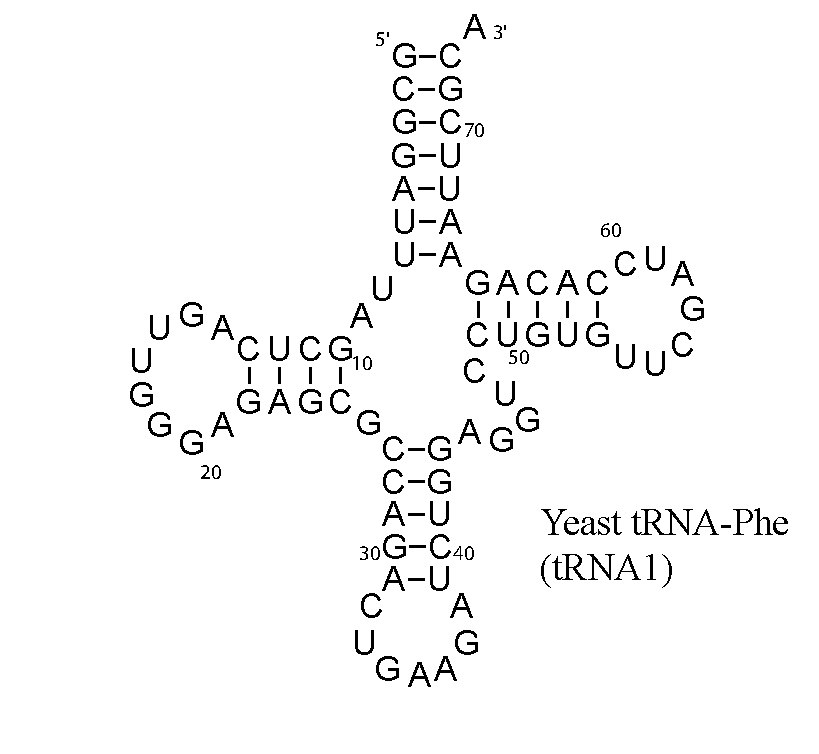
\includegraphics[scale=0.4]{Figures/trna1-DF6280}
\end{minipage}
\vspace{1em}

This is a simple example of a multiple RNA sequence alignment with
secondary structure annotation, in \emph{Stockholm format}.  Stockholm
format, the native alignment format used by HMMER and Infernal and the
Pfam and Rfam databases, is documented in detail later in the guide in
section~\ref{section:formats}.

For now, what you need to know about the key features of the input file is:
\begin{itemize}
\item The alignment is in an interleaved format.
Lines consist of a name, followed by an aligned sequence;
long alignments are split into blocks separated by blank lines.
\item Each sequence must have a unique name that has zero spaces in it. (This is important!)
\item For residues, any one-letter IUPAC nucleotide code is accepted,
      including ambiguous nucleotides. Case is ignored; residues
      may be either upper or lower case.
\item Gaps are indicated by the characters \otext{.}, \otext{\_}, -, or \verb+~+.
      (Blank space is not allowed.)
\item A special line starting with \otext{\#=GC SS\_cons} indicates
      the secondary structure consensus. Gap characters annotate
      unpaired (single-stranded) columns. Base pairs are indicated
      by any of the following pairs: \otext{<>}, \otext{()}, \otext{[]},
      or \otext{\{\}}. No pseudoknots are allowed; the
      open/close-brackets notation is only unambiguous for strictly
      nested base-pairing interactions.
      For more on secondary structure annotation see the WUSS format
      description in section~\ref{section:formats}.
\item The alignment begins with the special tag line
      \otext{\# STOCKHOLM 1.0}, and ends with \otext{//}.
      Stockholm alignments
      can be concatenated to create an alignment database flatfile
      containing many alignments.
\end{itemize}

The \prog{cmbuild} command builds a covariance model from an alignment (or
CMs for each of many alignments in a Stockholm file), and saves the
CM(s) in a file. For example, type:

\user{cmbuild tRNA5.cm tutorial/tRNA5.sto}

and you'll see some output that looks like:

\begin{sreoutput}
# cmbuild :: covariance model construction from multiple sequence alignments
# INFERNAL 1.1 (October 2013)
# Copyright (C) 2013 Howard Hughes Medical Institute.
# Freely distributed under the GNU General Public License (GPLv3).
# - - - - - - - - - - - - - - - - - - - - - - - - - - - - - - - - - - - -
# CM file:                                            tRNA5.cm
# alignment file:                                     ../../tutorial/tRNA5.sto
# - - - - - - - - - - - - - - - - - - - - - - - - - - - - - - - - - - - -
#                                                                      rel entropy
#                                                                      -----------
# idx    name                     nseq eff_nseq   alen  clen  bps bifs    CM   HMM description
# ------ -------------------- -------- -------- ------ ----- ---- ---- ----- ----- -----------
       1 tRNA5                       5     3.73     74    72   21    2 0.783 0.489 
#
# CPU time: 0.57u 0.00s 00:00:00.56 Elapsed: 00:00:00.57
\end{sreoutput}

If your input file had contained more than one alignment, you'd get
one line of output for each model. The information on these lines is
almost self-explanatory. The \otext{tRNA5} alignment consisted of 5
%  VERIFY WHEN UPDATING                                           ^
sequences with 74 aligned columns. Infernal turned it into a model of
%              ^^
72 consensus positions, which means it defined 2 gap-containing
%^                                             ^
alignment columns to be insertions relative to consensus. The 5
%                                                             ^
sequences were only counted as an ``effective'' total sequence number
(\otext{eff\_nseq}) of 3.73. The model includes 21 basepairs and 2
%                      ^^^^                     ^^               ^
bifurcations. The model ended up with a relative entropy per position
(\otext{rel entropy, CM}; information content) of 0.783 bits. If the
%                                                 ^^^^^
secondary structure information of the model were ignored the relative
entropy per position (\otext{rel entropy, HMM}) would be 0.489 bits.
%                                                        ^^^^^         
This output format is rudimentary. Infernal knows quite a bit more
information about what it's done to build this CM, but it's not
displaying it. You don't need to know more to be able to use the
model, so we can press on here. Model construction is described in
more detail in section~\ref{section:cmbuild}.

The new CM was saved to \otext{tRNA5.cm}. You can look at it
(e.g. \otext{> more tRNA5.cm}) if you like, but it isn't really designed
to be human-interpretable. You can treat \otext{.cm} files as compiled
models of your RNA alignment. The Infernal ASCII save file format is
defined in Section~\ref{section:formats}.

\subsubsection{Step 2: calibrate the model with cmcalibrate}

The next step is to ``calibrate'' the model. This step must be
performed prior to using your model for database searches with
\prog{cmsearch} or \prog{cmscan}. In this step, statistical parameters
necessary for reporting E-values (expectation values) are estimated
and stored in the CM file. When \prog{cmsearch} or \prog{cmscan} is
later used for a database search and a hit with score $x$ is found,
the E-value of that hit is the number of hits expected to score $x$ or
more just by chance (given the size of the search you're performing).

\emph{Importantly, if you're not going to use a model for database
search, there is no need to calibrate it.} For example, if you are
only going to use a model to create structurally annotated multiple
alignments of a large family like small subunit ribosomal RNA, don't
waste time calibrating it. \prog{cmsearch} and \prog{cmscan} are the
only Infernal programs that use E-values, so if you're not going to
use them then don't calibrate your model.

Unfortunately, CM calibration takes a long time because fairly long
random sequences must be searched to determine the expected
distribution of hit scores against nonhomologous sequences, and none
of the search acceleration heuristics described in
section~\ref{section:pipeline} can be used because they rely on
primary sequence similarity which is absent in random sequence.

The amount of time required for calibration varies widely, but
depends mainly on the size of the RNA family being modeled.
So you can know what kind of a wait you're in for, the
\prog{cmcalibrate} has a \otext{--forecast} option which reports an
estimate of the running time. To get an estimate for the tRNA model, do:

\user{cmcalibrate --forecast tRNA5.cm}\\

You should see something like this:

\begin{sreoutput}
# cmcalibrate :: fit exponential tails for CM E-values
# INFERNAL 1.1 (October 2013)
# Copyright (C) 2013 Howard Hughes Medical Institute.
# Freely distributed under the GNU General Public License (GPLv3).
# - - - - - - - - - - - - - - - - - - - - - - - - - - - - - - - - - - - -
# CM file:                                     tRNA5.cm
# forecast mode (no calibration):              on
# - - - - - - - - - - - - - - - - - - - - - - - - - - - - - - - - - - - -
#
# Forecasting running time for CM calibration(s) on 8 cpus:
#
#                          predicted
#                       running time
# model name            (hr:min:sec)
# --------------------  ------------
  tRNA5                     00:07:18
#
# CPU time: 0.30u 0.00s 00:00:00.30 Elapsed: 00:00:00.31
[ok]
\end{sreoutput}

The header comes first, telling you what program you ran, on what file
and with what options. This calibration will use 8 CPUs, your output
may vary depending on how many cores you have available on the machine
you're using. (If you are planning to use MPI to parallelize the
calibration (see the Installation section), you can specify the number
of CPUs for the time estimate as \otext{<n>} with the
\otext{--nforecast <n>} option.) Using 8 CPUs, \prog{cmcalibrate}
estimates the time required for calibration on the machine I'm using
at about seven minutes.

Feel free to perform the calibration yourself if you'd like (with the
command \otext{cmcalibrate tRNA5.cm}). However, we've included the file
\otext{tRNA5.c.cm}, an already calibrated version of \otext{tRNA5.cm},
for you to use if you don't want to wait. To use this calibrated
model, copy over the \otext{tRNA5.cm} file you just made with the
calibrated version:
 
\user{cp tutorial/tRNA5.c.cm tRNA5.cm}\\
 
\subsubsection{Step 3: search a sequence database with cmsearch}

You can now use your tRNA model to search for tRNA homologs in a
database. The file \otext{mrum-genome.fa} is the genome sequence of the
archaeon \emph{Methanobrevibacter rumanitium} (accession:
\otext{NC\_13790.1}). We'll use this file as our database. To perform
the search:

\user{cmsearch tRNA5.cm tutorial/mrum-genome.fa}\\
% tutorial regression: tRNA5-search.out

As before, the first section is the header, telling you what program
your ran, on what, and with what options:

\begin{sreoutput}
# cmsearch :: search CM(s) against a sequence database
# INFERNAL 1.1 (October 2013)
# Copyright (C) 2013 Howard Hughes Medical Institute.
# Freely distributed under the GNU General Public License (GPLv3).
# - - - - - - - - - - - - - - - - - - - - - - - - - - - - - - - - - - - -
# query CM file:                         tRNA5.cm
# target sequence database:              tutorial/mrum-genome.fa
# number of worker threads:              8
# - - - - - - - - - - - - - - - - - - - - - - - - - - - - - - - - - - - -
\end{sreoutput}

The second section is a list of ranked top hits (sorted by E-value,
most significant hit first):

\begin{sreoutput}
 rank     E-value  score  bias  sequence      start     end   mdl trunc   gc  description
 ----   --------- ------ -----  ----------- ------- -------   --- ----- ----  -----------
  (1) !   1.3e-18   71.5   0.0  NC_013790.1  362026  361955 -  cm    no 0.50  Methanobrevibacter ruminantium M1 chromosome, complete genome
  (2) !   3.3e-18   70.2   0.0  NC_013790.1 2585265 2585193 -  cm    no 0.60  Methanobrevibacter ruminantium M1 chromosome, complete genome
  (3) !     9e-18   68.8   0.0  NC_013790.1  762490  762562 +  cm    no 0.67  Methanobrevibacter ruminantium M1 chromosome, complete genome
  (4) !     9e-18   68.8   0.0  NC_013790.1 2041704 2041632 -  cm    no 0.67  Methanobrevibacter ruminantium M1 chromosome, complete genome
  (5) !   2.5e-17   67.4   0.0  NC_013790.1 2351254 2351181 -  cm    no 0.62  Methanobrevibacter ruminantium M1 chromosome, complete genome
  (6) !     3e-17   67.2   0.0  NC_013790.1  735136  735208 +  cm    no 0.59  Methanobrevibacter ruminantium M1 chromosome, complete genome
  (7) !   5.2e-17   66.4   0.0  NC_013790.1 2186013 2185941 -  cm    no 0.53  Methanobrevibacter ruminantium M1 chromosome, complete genome
  (8) !   1.6e-16   64.8   0.0  NC_013790.1 2350593 2350520 -  cm    no 0.66  Methanobrevibacter ruminantium M1 chromosome, complete genome
  (9) !   2.8e-16   64.1   0.0  NC_013790.1 2585187 2585114 -  cm    no 0.59  Methanobrevibacter ruminantium M1 chromosome, complete genome
 (10) !   9.1e-16   62.5   0.0  NC_013790.1  662185  662259 +  cm    no 0.61  Methanobrevibacter ruminantium M1 chromosome, complete genome
 (11) !   1.2e-15   62.1   0.0  NC_013790.1  360887  360815 -  cm    no 0.55  Methanobrevibacter ruminantium M1 chromosome, complete genome
 (12) !   1.6e-15   61.7   0.0  NC_013790.1 2350984 2350911 -  cm    no 0.53  Methanobrevibacter ruminantium M1 chromosome, complete genome
 (13) !   3.3e-15   60.7   0.0  NC_013790.1 2186090 2186019 -  cm    no 0.54  Methanobrevibacter ruminantium M1 chromosome, complete genome
 (14) !   4.1e-15   60.4   0.0  NC_013790.1 2680159 2680233 +  cm    no 0.67  Methanobrevibacter ruminantium M1 chromosome, complete genome
 (15) !   7.9e-15   59.5   0.0  NC_013790.1 2749839 2749768 -  cm    no 0.53  Methanobrevibacter ruminantium M1 chromosome, complete genome
 (16) !   7.9e-15   59.5   0.0  NC_013790.1 2749945 2749874 -  cm    no 0.53  Methanobrevibacter ruminantium M1 chromosome, complete genome
 (17) !   9.8e-15   59.2   0.0  NC_013790.1  361676  361604 -  cm    no 0.51  Methanobrevibacter ruminantium M1 chromosome, complete genome
 (18) !     1e-14   59.2   0.0  NC_013790.1 2585073 2584999 -  cm    no 0.60  Methanobrevibacter ruminantium M1 chromosome, complete genome
 (19) !   1.1e-14   59.1   0.0  NC_013790.1 2130422 2130349 -  cm    no 0.59  Methanobrevibacter ruminantium M1 chromosome, complete genome
 (20) !   1.2e-14   58.9   0.0  NC_013790.1  546056  545947 -  cm    no 0.61  Methanobrevibacter ruminantium M1 chromosome, complete genome
 (21) !   3.9e-14   57.3   0.0  NC_013790.1  361915  361844 -  cm    no 0.42  Methanobrevibacter ruminantium M1 chromosome, complete genome
 (22) !   5.1e-14   57.0   0.0  NC_013790.1   97724   97795 +  cm    no 0.49  Methanobrevibacter ruminantium M1 chromosome, complete genome
 (23) !   6.1e-14   56.7   0.0  NC_013790.1 2350717 2350646 -  cm    no 0.68  Methanobrevibacter ruminantium M1 chromosome, complete genome
 (24) !     8e-14   56.3   0.0  NC_013790.1 1873887 1873815 -  cm    no 0.64  Methanobrevibacter ruminantium M1 chromosome, complete genome
 (25) !   1.4e-13   55.6   0.0  NC_013790.1  360730  360659 -  cm    no 0.40  Methanobrevibacter ruminantium M1 chromosome, complete genome
 (26) !   3.5e-13   54.3   0.0  NC_013790.1 2680310 2680384 +  cm    no 0.52  Methanobrevibacter ruminantium M1 chromosome, complete genome
 (27) !   3.6e-13   54.3   0.0  NC_013790.1 2664806 2664732 -  cm    no 0.60  Methanobrevibacter ruminantium M1 chromosome, complete genome
 (28) !   3.6e-13   54.3   0.0  NC_013790.1  361061  360989 -  cm    no 0.41  Methanobrevibacter ruminantium M1 chromosome, complete genome
 (29) !   7.5e-13   53.3   0.0  NC_013790.1 2130335 2130262 -  cm    no 0.55  Methanobrevibacter ruminantium M1 chromosome, complete genome
 (30) !   7.6e-13   53.3   0.0  NC_013790.1 2151672 2151745 +  cm    no 0.65  Methanobrevibacter ruminantium M1 chromosome, complete genome
 (31) !   2.9e-12   51.4   0.0  NC_013790.1  319297  319370 +  cm    no 0.62  Methanobrevibacter ruminantium M1 chromosome, complete genome
 (32) !   3.7e-12   51.1   0.0  NC_013790.1  361753  361679 -  cm    no 0.55  Methanobrevibacter ruminantium M1 chromosome, complete genome
 (33) !   3.8e-12   51.1   0.0  NC_013790.1  360983  360912 -  cm    no 0.50  Methanobrevibacter ruminantium M1 chromosome, complete genome
 (34) !   5.9e-12   50.5   0.0  NC_013790.1  361456  361383 -  cm    no 0.50  Methanobrevibacter ruminantium M1 chromosome, complete genome
 (35) !   7.4e-12   50.1   0.0  NC_013790.1  362798  362727 -  cm    no 0.51  Methanobrevibacter ruminantium M1 chromosome, complete genome
 (36) !   8.7e-12   49.9   0.0  NC_013790.1  917722  917793 +  cm    no 0.61  Methanobrevibacter ruminantium M1 chromosome, complete genome
 (37) !   1.1e-11   49.7   0.0  NC_013790.1 2583869 2583798 -  cm    no 0.51  Methanobrevibacter ruminantium M1 chromosome, complete genome
 (38) !   1.3e-11   49.4   0.0  NC_013790.1  362324  362252 -  cm    no 0.51  Methanobrevibacter ruminantium M1 chromosome, complete genome
 (39) !   1.3e-11   49.3   0.0  NC_013790.1  360811  360740 -  cm    no 0.42  Methanobrevibacter ruminantium M1 chromosome, complete genome
 (40) !   4.3e-11   47.7   0.0  NC_013790.1 1160526 1160609 +  cm    no 0.60  Methanobrevibacter ruminantium M1 chromosome, complete genome
 (41) !   9.8e-11   46.6   0.0  NC_013790.1  362403  362331 -  cm    no 0.49  Methanobrevibacter ruminantium M1 chromosome, complete genome
 (42) !   1.1e-10   46.5   0.0  NC_013790.1 2327124 2327042 -  cm    no 0.63  Methanobrevibacter ruminantium M1 chromosome, complete genome
 (43) !   1.2e-10   46.4   0.0  NC_013790.1  995344  995263 -  cm    no 0.49  Methanobrevibacter ruminantium M1 chromosome, complete genome
 (44) !   2.3e-10   45.5   0.0  NC_013790.1  256772  256696 -  cm    no 0.57  Methanobrevibacter ruminantium M1 chromosome, complete genome
 (45) !   2.5e-10   45.3   0.0  NC_013790.1 2584830 2584758 -  cm    no 0.64  Methanobrevibacter ruminantium M1 chromosome, complete genome
 (46) !   6.1e-10   44.1   0.0  NC_013790.1 2351071 2350997 -  cm    no 0.59  Methanobrevibacter ruminantium M1 chromosome, complete genome
 (47) !   6.5e-10   44.0   0.0  NC_013790.1  362552  362482 -  cm    no 0.55  Methanobrevibacter ruminantium M1 chromosome, complete genome
 (48) !   5.2e-09   41.2   0.0  NC_013790.1 1064775 1064858 +  cm    no 0.63  Methanobrevibacter ruminantium M1 chromosome, complete genome
 (49) !   1.2e-08   40.0   0.0  NC_013790.1  361222  361150 -  cm    no 0.45  Methanobrevibacter ruminantium M1 chromosome, complete genome
 (50) !   1.2e-08   40.0   0.0  NC_013790.1  361369  361297 -  cm    no 0.60  Methanobrevibacter ruminantium M1 chromosome, complete genome
 (51) !   4.8e-08   38.1   0.0  NC_013790.1  361596  361513 -  cm    no 0.61  Methanobrevibacter ruminantium M1 chromosome, complete genome
 (52) !   3.2e-07   35.5   0.0  NC_013790.1 1913310 1913227 -  cm    no 0.64  Methanobrevibacter ruminantium M1 chromosome, complete genome
 (53) !   2.6e-06   32.7   0.0  NC_013790.1  363464  363381 -  cm    no 0.51  Methanobrevibacter ruminantium M1 chromosome, complete genome
 (54) !     3e-06   32.5   0.0  NC_013790.1 2584954 2584872 -  cm    no 0.58  Methanobrevibacter ruminantium M1 chromosome, complete genome
 ------ inclusion threshold ------
 (55) ?     0.027   20.0   0.0  NC_013790.1  363803  363716 -  cm    no 0.50  Methanobrevibacter ruminantium M1 chromosome, complete genome
 (56) ?       3.4   13.4   0.0  NC_013790.1  984373  984304 -  cm    no 0.53  Methanobrevibacter ruminantium M1 chromosome, complete genome
\end{sreoutput}

The first number is the rank of each hit\footnote{Ranks of hits are in
  parantheses to make it easy to jump to/from an entry in the hit list
  and the hit alignment section, described later.}. Next comes either a
\otext{!} or \otext{?} symbol and then the \emph{E-value} of the hit.
The E-value is the statistical significance of the hit: the number of
hits we'd expect to score this highly in a database of this size
(measured by the total number of nucleotides) if the database
contained only nonhomologous random sequences. The lower the E-value,
the more significant the hit. The \otext{!} or \otext{?} that
precedes the E-value indicates whether the hit does (\otext{!}) or
does not (\otext{?}) satisfy the inclusion threshold for the search.
Inclusion thresholds are used to determine what matches should be
considered to be ``true'', as opposed to reporting thresholds that
determine what matches will be reported (often including the top of
the noise, so you can see what interesting sequences might be getting
tickled by your search). By default, inclusion thresholds usually
require an E-value of 0.01 or less, and reporting E-value thresholds
are set to 10.0, but these can be changed (see the manual page for
\prog{cmsearch} toward the end of guide).

The E-value is based on the \emph{bit score}, which is in the next
column. This is the log-odds score for the hit. Some people like to
see a bit score instead of an E-value, because the bit score doesn't
depend on the size of the sequence database, only on the covariance
model and the target sequence.

The next number, the \emph{bias}, is a correction term for biased
sequence composition that has been applied to the sequence bit
score. Infernal uses an alternative null model we call \emph{null3},
described more in section~\ref{section:pipeline}, to determine the bias
bit score correction. The bias correction is often very small and is
only reported to one decimal place, after rounding. For all hits in
this example search the bias column reads 0.0 bits, indicating that
the correction is less than 0.05 bits. On very biased sequences this
correction can become significant and is helpful for lowering the
score of high-scoring false positives that achieve high scores solely
due to their biased composition. 

Next comes the target sequence name the hit is in, and the start and
end positions of the hit within the sequence. Hits can occur on either
the top (Watson) or bottom (Crick) strand of the target
sequence\footnote{You can search either only the top strand with the
\otext{--toponly} or bottom strand with the \otext{--bottomonly} options
to \prog{cmsearch} and \prog{cmscan}.}, so the start position may be
less than (if hit is on the top strand) or greater than (if hit is on
the bottom strand) the end position. After the end position, comes a single
\otext{+} or \otext{-} symbol, indicating whether the hit is on the
top (\otext{+}) or bottom (\otext{-}) strand (solely for convenience -
so you don't have to look at the start and end positions to determine
the strand the hit is on).

After the strand symbol comes the model field, which indicates whether
the hit was found using either the CM (\otext{cm}) or a profile HMM
built from the CM (\otext{hmm}). This field is necessary because for
models with zero basepairs, \prog{cmsearch} (and \prog{cmscan}) use a
profile HMM instead of a CM for final hit scoring. This is done for
reasons of speed and efficiency, because profile HMM algorithms are
more efficient than CM ones and a CM with zero basepairs is
essentially equivalent to a profile HMM. In this example, since our
tRNA model does include basepairs, \prog{cmsearch} used a CM to score
all hits and so all hits have \prog{cm} for this column. There's an
example later in the tutorial of hits found with a profile HMM.

The next column indicates whether the hit is \emph{truncated} or
not. Infernal uses special versions of its CM dynamic programming
algorithms to allow detection of structural RNAs that have been
truncated due to missing data at the beginning and/or end of a target
sequence. Truncated hits are most common in databases that include
single reads from shotgun sequencing projects. Since our database is a
complete genome, we don't expect any hits to be truncated due to
missing data. For all hits the ``trunc'' column reads
``no'' indicating that, as expected, none of the hits are
truncated. There are examples of truncated hits in the next exercise
which uses \prog{cmscan}. Section~\ref{section:pipeline} describes how
Infernal detects and aligns truncated hits in more detail.

The next column reports the GC fraction of the hit. This is the
fraction of residues in the target sequence hit that are either G or C
residues. The GC fraction is included as an additional indication of
the level of sequence bias of the hit. Some expert users may be aided
by this number when deciding if they believe a hit is a real homolog
or a false positive.

Finally comes the description of the sequence, if any. This
description is propogated from the input target sequence file.

After the hit list comes the hit alignments section. Each hit in 
the hit list will have a corresponding entry in this section, in the
same order. As an illustrative example, let's take a look at
hit number 43. First, take a look at the first four lines for this
hit: 

\begin{sreoutput}
>> NC_013790.1  Methanobrevibacter ruminantium M1 chromosome, complete genome
 rank     E-value  score  bias mdl mdl from   mdl to       seq from      seq to       acc trunc   gc
 ----   --------- ------ ----- --- -------- --------    ----------- -----------      ---- ----- ----
 (43) !   1.2e-10   46.4   0.0  cm        1       72 []      995344      995263 - .. 0.93    no 0.49
\end{sreoutput}

The first line of each hit alignment begins with \otext{>>} followed
by a single space, the name of the target sequence, then two spaces
and the description of the sequence, if any. Next comes a set of
tabular fields that is partially redundant with the information in the
hit list. The first five columns are the same as in the hit list. The
next column reports the type of model used for the alignment, as
described above for the hit list. The next four columns report the
boundaries of the alignment with respect to the query model (``mdl
from'' and ``mdl to'') and the target sequence (``seq from'' and ``seq
to''). Following the ``seq to'' column is a \otext{+} or \otext{-}
symbol indicating whether the hit is on the top (\otext{+}) or bottom
(\otext{-}) strand.

It's not immediately easy to tell from the ``to'' coordinate whether
the alignment ended internally in the query model or target sequence,
versus ran all the way (as in a full-length global alignment) to the
end(s). To make this more readily apparent, with each pair of query
and target endpoint coordinates, there's also a little symbology. For
the normal case of a non-truncated hit: \otext{..} means both ends of
the alignment ended internally, and \otext{[]} means both ends of the
alignment were full-length flush to the ends of the query or target,
and \otext{[.}  and \otext{.]} mean only the left (5') or right (3') end
was flush/full length. For truncated hits, the symbols are the same
except that either the first and/or the second symbol will be a
\verb+~+ for the query and target. If the first symbol is \verb+~+
then the left end of the alignment is truncated because the 5' end of
the hit is predicted to be missing (extend beyond the beginning of the
target sequence). Similarly, if the second symbol is \verb+~+ then the
right end of the alignment is truncated because the 3' end of the hit
is predicted to be missing (extend beyond the end of the target
sequence). These two symbols occur just after the ``mdl to'' column for
the query, and after the strand \otext{+} or \otext{-} symbol for the
target sequence.

The next column is labeled ``acc'' and is the average posterior
probability of the aligned target sequence residues; effectively, the
expected accuracy per residue of the alignment.

The final two columns indicate whether the hit is truncated or not and
the GC fraction of the hit. These are redundant with the columns of
the same name in the hit list, described above.

Next comes the alignment display. This is an ``optimal
posterior accuracy'' alignment \citep{Holmes98}, which means it is the
alignment with the maximal summed posterior probability of all
aligned residues. Take a look at the alignment for hit number 43:

% tutorial regression: tRNA5-search.out
\begin{sreoutput}
                                 v         v                                                            NC
                     (((((((,,<<<<______.._>>>>,<<<<<_______>>>>>,,,........,,<<<<<_______>>>>>))))))): CS
        tRNA5      1 gCcggcAUAGcgcAgUGGu..AgcgCgccagccUgucAagcuggAGg........UCCgggGUUCGAUUCcccGUgccgGca 72    
                     :::G:CAUAGCG AG GGU  A CGCG:CAG:CU +++A:CUG: G+        UC:GGGGUUCGA UCCCC:UG:C:::A
  NC_013790.1 995344 AGAGACAUAGCGAAGCGGUcaAACGCGGCAGACUCAAGAUCUGUUGAuuaguucuUCAGGGGUUCGAAUCCCCUUGUCUCUA 995263
                     **********************************************9444444445************************** PP
\end{sreoutput}

The alignment contains six lines. Start by looking at the second line
which ends with \otext{CS}.  The line shows the predicted secondary
structure of the target sequence. The format is a little fancier and
more informative than the simple least-common-denominator format we
used in the input alignment file. It's designed to make it easier to
see the secondary structure by eye. The format is described in detail
later (see WUSS format in section~\ref{section:formats}); for now,
here's all you need to know. Basepairs in simple stem loops are
annotated with \otext{<>} characters. Basepairs enclosing
multifurcations (multiple stem loops) are annotated with \otext{()},
such as the tRNA acceptor stem in this example. In more complicated
structures, \otext{[]} and \otext{\{\}} annotations also show up, to
reflect deeper nestings of multifurcations. For single stranded
residues, \otext{\_} characters mark hairpin loops; \otext{-}
characters mark interior loops and bulges; \otext{,} characters mark
single-stranded residues in multifurcation loops; and \otext{:}
characters mark single stranded residues external to any secondary
structure. Insertions relative to this consensus are annotated by a
\otext{.} character.

The line above the \otext{CS} line ends with \otext{NC} and marks
negative scoring non-canonical basepairs in the alignment with a
\otext{v} character. All other positions of the alignment will be
blank\footnote{For anyone trying to parse this output, this means it
is possible for this line to be completely blank except for the
\otext{NC} trailer.} More specifically, the following ten types of
basepairs which are assigned a negative score by the model at their
alignment positions will be marked with a \otext{v}: \otext{A:A},
\otext{A:C}, \otext{A:G}, \otext{C:A}, \otext{C:C}, \otext{C:U},
\otext{G:A}, \otext{G:G}, \otext{U:U}, and \otext{U:C}. The \otext{NC}
annotation makes it easy to quickly identify suspicious basepairs in
a hit. Importantly, the \otext{NC} annotation will only be present in
CM hit alignments (``mdl'' column reads ``cm'') and will be absent in
HMM hit alignments (``mdl'' column reads ``hmm'') because basepairs
are not scored by an HMM.

The third line shows that consensus of the query model. The highest
scoring residue sequence is shown. Upper case residues are highly
conserved. Lower case residues are weakly conserved or unconserved.
Dots (\otext{.}) in this line indicate insertions in the target
sequence with respect to the model.

The fourth line shows where the alignment score is coming from. For a
consensus basepair, if the observed pair is the highest-scoring
possible pair according to the consensus, both residues are shown in
upper case; if a pair has a score of $\geq 0$, both residues are
annotated by : characters (indicating an acceptable compensatory
basepair); else, there is a space, indicating that a negative
contribution of this pair to the alignment score. Note that the 
\otext{NC} line will only mark a subset of these negative scoring
pairs with a \otext{v}, as discussed above.
For a single-stranded consensus residue, if the observed residue is
the highest scoring possibility, the residue is shown in upper case;
if the observed residue has a score of $\geq 0$, a \otext{+} character
is shown; else there is a space, indicating a negative contribution to
the alignment score. Importantly, for HMM hits (``mdl'' column reads
``hmm''), \emph{all} positions are considered single stranded, since
an HMM scores each half of a basepair independently.

The fifth line, beginning with \otext{NC\_013790.1} is
the target sequence. Dashes (\otext{-}) in this line indicate deletions
in the target sequence with respect to the model.

The bottom line is new to version 1.1 of Infernal. This represents the
posterior probability (essentially the expected accuracy) of each
aligned residue. A 0 means 0-5\%, 1 means 5-15\%, and so on; 9 means
85-95\%, and a \otext{*} means 95-100\% posterior probability. You can
use these posterior probabilities to decide which parts of the
alignment are well-determined or not. You'll often observe, for
example, that expected alignment accuracy degrades around locations of
insertion and deletion, which you'd intuitively expect.

Alignments for some searches may be formatted slightly differently
than this example. Longer alignments to longer models will be broken
up into blocks of six lines each - this alignment was short enough to
be entirely contained within a single block.  If your model was built
with the \otext{--hand} option in \prog{cmbuild}, then an additional
line will be included in each block, with RF annotation.  If the model
used for the alignment was an HMM (the ``mdl'' column reads ``hmm'')
then the \otext{NC} line will be absent from each alignment
block. We'll see example of all three of these cases later in the
tutorial.

After hit number 43, there's 13 more hit alignments for hits number 44
through 56. 

Finally, at the bottom of the file, you'll see some summary
statistics. For example, at the bottom of the tRNA search output,
you'll find something like:

\begin{sreoutput}
Internal CM pipeline statistics summary:
----------------------------------------
Query model(s):                                                  1  (72 consensus positions)
Target sequences:                                                1  (5874406 residues searched)
Target sequences re-searched for truncated hits:                 1  (360 residues re-searched)
Windows   passing  local HMM SSV           filter:           11200  (0.2111); expected (0.35)
Windows   passing  local HMM Viterbi       filter:                  (off)
Windows   passing  local HMM Viterbi  bias filter:                  (off)
Windows   passing  local HMM Forward       filter:             137  (0.002691); expected (0.005)
Windows   passing  local HMM Forward  bias filter:             134  (0.002621); expected (0.005)
Windows   passing glocal HMM Forward       filter:              87  (0.001923); expected (0.005)
Windows   passing glocal HMM Forward  bias filter:              87  (0.001923); expected (0.005)
Envelopes passing glocal HMM envelope defn filter:             100  (0.001342); expected (0.005)
Envelopes passing  local CM  CYK           filter:              60  (0.0007631); expected (0.0001)
Total CM hits reported:                                         56  (0.0007205); includes 0 truncated hit(s)

# CPU time: 2.21u 0.02s 00:00:02.23 Elapsed: 00:00:00.64
//
\end{sreoutput}

This gives you some idea of what's going on in Infernal's acceleration
pipeline. You've got one query CM, and the database has one target
%                    ^                                  ^
sequence. The search examined 5,874,406 residues, even though the
%                             ^^^^^^^^^
actual target sequence length is only half that, because both the top
and bottom strand of each target is searched. 360 of those residues
%                                             ^^^
were searched more than once in an effort to find truncated
hits. Ignore this for the moment, we'll revisit this later after
discussing the filter pipeline (in the subsection entitled ``Truncated
RNA detection'' below).

Each sequence goes through a multi-stage filter pipeline of four
scoring algorithms called SSV, Viterbi, Forward\footnote{Actually two
  separate Forward based filters are used, the first with the profile
  HMM in local mode and the next with the profile HMM in global
  mode. There's more detail on this in
  section~\ref{section:pipeline}.}, and CYK in order of increasing
sensitivity and increasing computational requirement. The filter
pipeline is the topic of section~\ref{section:pipeline} of this guide
but briefly, SSV, Viterbi and Forward are profile HMM algorithms which
are more efficient than CM algorithms. These three algorithms are the
same ones used by HMMER3 and are the main reason that version 1.1 of
Infernal is so much faster than previous versions. For these HMM
stages, Infernal uses a filter profile HMM that was constructed
simultaneously with the CM, from the same training alignment in
\prog{cmbuild}, and stored in the CM file. CYK is a CM scoring
algorithm, so it's slow, but it is accelerated using banded dynamic
programming with bands derived from an HMM alignment. Subsequences
that survive all filters are finally scored with the CM Inside
algorithm, agains using HMM bands. Subsequences that score
sufficiently high with Inside are then aligned using the optimal
posterior accuracy algorithm and displayed.

The score thresholds for a subsequence surviving each HMM filter stage
are dependent on the search space size (sequence database size for
\prog{cmsearch}). This differs from HMMER3 which always uses the same
filter thresholds. In general, the larger the search
space the more strict the thresholds are, because a hit must have a
higher bit score to have a significant E-value.  In this case, the
database is relatively small so the filter thresholds have been set
relatively loosely. The SSV filter has been configured to allow
subsequences with a P-value of $\leq 0.35$ through
%                                   ^^^^^^
the SSV score filter (thus, if the database contained no homologs and
P-values were accurately calculated, the highest scoring 35\% of the
%                                           ^^^^
residues will pass the filter). Here, about 21\% of the database in
%                                           ^^^^
11,200 separate windows got through the SSV filter. For a database of
%^^^^^
this size, the local Viterbi filter is turned off.  The local Forward filter
is set to allow an expected 0.5\% of the database survive. Here about
%                           ^^^^
0.3\% survives in 137 windows. Next, each surviving window is checked
%^^
to see if the target sequence is ``obviously'' so biased in its
composition that it's unlikely to be a true homolog. This is called
the ``bias filter''\footnote{There's also a bias filter step used in
  the local Viterbi filter stage, when it is used.} and applying a bit
score correction to previous filter's score for each window and
recomputing the P-value. Three of the 137 windows fail to pass
%                        ^^^^^        ^^^
the local Forward bias filter stage. Next, the Forward algorithm is
used to score each window again, but this time with the HMM configured
in glocal mode requiring a full length alignment to the
model\footnote{The use of glocal Forward is another important
  difference between Infernal and HMMER3's (v3.0) pipeline. HMMER v3.0
  only uses local HMM algorithms.}  As with the local stage, an
expected 0.5\% of the database is expected to survive. In this case,
87 of the 134 windows, comprising about 0.2\% of the database,
%^        ^^^
survive. The bias filter is run again, this time applying a correction
to the glocal Forward scores. For this search, 0 windows are removed at
this stage. The envelope definition stage is next. This stage is very
similar to the HMMER3 domain definition stage, with the difference
that the HMM is configured in glocal rather than local mode. In this
stage, the Forward and Backward algorithms are used to identify zero
or more hit envelopes in each window, where each envelope contains one
putative hit.  Often residues at the beginning and ends of windows are
determined to be nonhomologous and are not included in the
envelope. In this search, 100 envelopes are defined within the 87
%                         ^^^                                  ^^
windows. Note that the envelopes comprise only about 70\% of the
%                                                    ^^^
residues from the 87 windows, indicated by the drop of 0.1923\% to
%                                                      ^^^^^^^^
0.1342\%.
%%^^^^

After hit envelopes have been defined with the filter HMM, the two
remaining stages of the pipeline use the CM to score both the
conserved sequence and structure of each possible hit. In both of
these stages, constraints are derived from an HMM alignment of the
envelope and enforced as \emph{bands} on the CM dynamic programming
matrices (more on this in section~\ref{section:pipeline}). In the
first CM stage, the CYK algorithm (which is the SCFG analog of the
Viterbi HMM algorithm) is used to determine the best scoring maximum
likelihood alignment of any subsequence in each envelope to the CM. If
this alignment has a P-value of $\leq 0.0001$ then the envelope
survives to the final round. The envelopes passed to the final stage
may be shorter than those examined during the CYK stage. Specifically,
envelopes are redefined as starting and ending at the first and final
residues for which at least one alignment exists with a P-value $\leq
0.001$.

In the final round, the Inside algorithm (the SCFG analog of the HMM
Forward algorithm) is used to define final hit boundaries and
scores. Hits with scores above the reporting threshold were output, as
described above. In this search there were 56 such hits.
%                                          ^^

Finally, the running time of the search is reported, in CPU time and
elapsed time. This search took about 1 second (wall
%                                    ^
clock time) (running on eight cores). 

\subsubsection{Truncated RNA detection}

Now, we come back to the topic of truncated hit detection.  As briefly
mentioned above, the pipeline statistics summary from our search above
reported that 360 residues were re-searched for truncated
%             ^^^
hits. Infernal explicitly looks at the 5' and 3' ends of target
sequences using specialized algorithms for detection of truncated
hits, in which part of the 5' and/or 3' end of the actual full length
sequence from the source organism's full genomic context is missing in
the input target sequence. Truncated hits will be most common in
sequence files consisting of unassembled sequencing reads. In our
search of the full archaeal genome above, no truncated hits were
found. However, there is an example of a truncated hit in the
\prog{cmscan} tutorial section below in a sequence from a metagenomics
sequencing survey.

Special dynamic programming algorithms are required for truncated hit
detection \citep{KolbeEddy09}, so sequences must be re-searched for
truncated hits after they are initially searched for standard
(non-truncated) hits. However, only the sequence ends must be
re-searched because Infernal assumes that only hits at sequence
terminii might be truncated. This is why our search above reported
that only 360 residues were re-searched for truncated hits. For each
%         ^^^
model, an expected maximum length of a hit\footnote{The expected
  maximum hit length is defined as the maximum of 1.25 times the
  consensus length of the model and the $W$ parameter computed with
  the QDB algorithm \citep{NawrockiEddy07}. $W$ is computed based on
  the transition probabilities of the model by \prog{cmbuild} and
  stored in the CM file.} 
is used to define the window length at the
beginning and end of each sequence which must be re-searched for
truncated hits. For our tRNA model the maximum expected length is
90, so exactly 360 residues were re-searched: the first and final 90
%^             ^^^                                                ^^
residues on the top strand, and the first and final 90 residues on
%                                                   ^^
the bottom strand.

There is one more aspect of truncated hit detection that is important
to mention here. Because Infernal expects that hit truncation only
occurs at the ends of sequences, 5' truncated hits are forced to start
at the first nucleotide of a sequence, 3' truncated hits are forced to
end at the final nucleotide of the sequence, and 5' \emph{and} 3'
truncated hits are forced to include the full sequence.

The annotation of truncated hits in \prog{cmsearch} output is slightly
different than for standard (non-truncated) hits. An example is
included in the next section below.

\subsection{Searching a CM database with a query sequence}

The \prog{cmscan} program is for annotating all the different
known/detectable RNAs in a given sequence. It takes a single query
sequence and a CM database as input. The CM database might be Rfam,
for example, or another collection of your choice. \prog{cmscan} is
new to version 1.1 of Infernal. It is designed to be useful for
sequence datasets from RNA-Seq experiments or metagenomics surveys,
for which one wants to know what families of RNAs are represented in
the sequence dataset.

\subsubsection{Step 1: create an CM database flatfile}

A CM ``database'' flatfile is simply a concatenation of individual CM
files. To create a database flatfile, you can either build and
calibrate individual CM files and concatenate them, or you can
concatenate Stockholm alignments and use \prog{cmbuild} to build a CM
database of all of them in one command, and then calibrate that
database with \prog{cmcalibrate}. Importantly, \prog{cmscan} can only
be used with calibrated CMs.

Let's create a tiny database called \otext{minifam.cm} containing the
tRNA model we've been working with, a 5S ribosomal RNA model, and a
Cobalamin riboswitch model. To save you time, calibrated versions of
the 5S and Cobalamin models are included in the \otext{tutorial/}
directory in the files \otext{5S\_rRNA.c.cm}, and
\otext{Cobalamin.c.cm}. These files were created using \prog{cmbuild}
and \prog{cmcalibrate} from the Rfam 10.1 seed alignments for 5S\_rRNA
(RF00001) and Cobalamin (RF00174), provided in
\otext{tutorial/5S\_rRNA.sto} and \otext{tutorial/Cobalamin.sto}. The
third model is the tRNA model from earlier in the tutorial 
(\otext{tRNA5.c.cm}). Feel free to build and calibrate these
models yourself if you'd like, but if you'd like to keep moving on
with the tutorial, use the pre-calibrated ones. To create the database,
simply concatenate the three provided files:

\user{cat tutorial/tRNA5.c.cm tutorial/5S\_rRNA.c.cm tutorial/Cobalamin.c.cm > minifam.cm}

\subsubsection{Step 2: compress and index the flatfile with cmpress}

The \prog{cmscan} program has to read a lot of CMs and their filter
HMMs in a hurry, and Infernal's ASCII flatfiles are bulky. To
accelerate this, \prog{cmscan} uses binary compression and indexing of
the flatfiles. To use \prog{cmscan}, you must first compress and
index your CM database with the \prog{cmpress} program:

\user{cmpress minifam.cm}

This will quickly produce:

\begin{sreoutput}
Working...    done.
Pressed and indexed 3 CMs and p7 HMM filters (3 names and 2 accessions).
Covariance models and p7 filters pressed into binary file:  minifam.cm.i1m
SSI index for binary covariance model file:                 minifam.cm.i1i
Optimized p7 filter profiles (MSV part)  pressed into:      minifam.cm.i1f
Optimized p7 filter profiles (remainder) pressed into:      minifam.cm.i1p
\end{sreoutput}

and you'll see these four new binary files in the directory. 

The \otext{tutorial} directory includes a copy of the
\otext{minifam.cm} file, which has already been pressed, so there
are example binary files \otext{tutorial/minifam.cm.i1\{m,i,f,p\}}
included in the tutorial.

Their format is ``proprietary'', which is an open source term of art
that means both ``We haven't found time to document them yet'' and ``We
still might decide to change them arbitrarily without telling you''.

\subsubsection{Step 3: search the CM database with cmscan}

Now we can analyze sequences using our CM database and
\prog{cmscan}. 

For example, the file \otext{tutorial/metag-example.fa} includes 3
sequences (whole genome shotgun sequencing reads) derived from samples
of ``whale fall'' carcasses in a metagenomics study
\citep{Tringe05}. These three sequences were chosen from the roughly
200,000 in the complete dataset because they include statistically
significant hits to the three models in our toy CM database.

To scan the sequences with our database: 

\user{cmscan minifam.cm tutorial/metag-example.fa}
%tutorial regression: metag-scan.out

The header and the first section of the output will look like:

\newpage

\begin{sreoutput}
# cmscan :: search sequence(s) against a CM database
# INFERNAL 1.1 (October 2013)
# Copyright (C) 2013 Howard Hughes Medical Institute.
# Freely distributed under the GNU General Public License (GPLv3).
# - - - - - - - - - - - - - - - - - - - - - - - - - - - - - - - - - - - -
# query sequence file:                   ../../tutorial/metag-example.fa
# target CM database:                    minifam.cm
# number of worker threads:              8
# - - - - - - - - - - - - - - - - - - - - - - - - - - - - - - - - - - - -

Query:       AAGA01015927.1  [L=943]
Description: Metagenome sequence AHAI1002.g1, whole genome shotgun sequence
Hit scores:
 rank     E-value  score  bias  modelname  start    end   mdl trunc   gc  description
 ----   --------- ------ -----  --------- ------ ------   --- ----- ----  -----------
  (1) !   3.3e-19   77.3   0.0  5S_rRNA       59    174 +  cm    no 0.66  5S ribosomal RNA
  (2) !   9.3e-19   62.4   0.0  tRNA5        229    302 +  cm    no 0.62  -
  (3) !     6e-16   53.5   0.0  tRNA5        314    386 +  cm    no 0.59  -
\end{sreoutput}

\prog{cmscan} has identified three putative RNAs in the first query
sequence, one 5S rRNA and two tRNAs. The output fields are in the
same order and have the same meaning as in \prog{cmsearch}'s output.

Before we move on, this is a good opportunity to point out an
important difference between \prog{cmsearch} and \prog{cmscan} related
to the size of the search space (often referred to in the code and in
this guide as the $Z$ parameter).  The size of the search space for
\prog{cmscan} is double the length of the current (single) query
sequence (doubled because we're searching both strands) multiplied by
the number of models in the CM database (here, 3; for a Rfam search,
on the order of 1000). Because each query sequence is probably a
different size this means $Z$ changes for each query sequence. In
\prog{cmsearch}, the size of the search space is double the summed
length of all sequences in the database (again, doubled because both
strands are searched). This means that E-values may differ even for
the same individual CM vs. sequence comparison, depending on how you
do the search. The search space size also affects what filter
thresholds \prog{cmsearch} or \prog{cmscan} will use, which is
discussed more in section~\ref{section:pipeline}.

Now back to the \prog{cmscan} results. What follows the ranked list of
three hits are the hit alignments. These are constructed and annotated
the same as in \prog{cmsearch}. The 5S alignment is:

\begin{widesreoutput}
                             v               v       v         v         v             v           vv                NC
                     (((((((((,,,,<<-<<<<<---<<--<<<<<<______.>>-->>>>-->>---->>>>>-->><<<-<<----<-<<-----<<____>>-- CS
         5S_rRNA   1 gcuuGcggcCAUAccagcgcgaAagcACcgGauCCCAUCc.GaACuCcgAAguUAAGcgcgcUugggCcagggUAGUAcuagGaUGgGuGAcCuC 94 
                     :CU:GC:G C UA:C+::G:G+   CACC:GA CCCAU C G ACUC:GAAG  AA C:C::U+G: CC+::G  G:A  + G  GGGU  CC C
  AAGA01015927.1  59 CCUGGCGGCCGUAGCGCGGUGGUCCCACCUGACCCCAUGCcGAACUCAGAAGUGAAACGCCGUAGCGCCGAUG--GUAGUGUG--GGGUCUCCCC 149
                     *************************************************************************..********..********** PP

                        vv         v v          NC
                     --->>->-->>->>>.))))))))): CS
         5S_rRNA  95 cUGggAAgaccagGu.gccgCaagcc 119
                      UG  A: A::AGG   C:GC:AG:C
  AAGA01015927.1 150 AUGCGAG-AGUAGGGaACUGCCAGGC 174
                     **99999.****************** PP
\end{widesreoutput}

After the three sequences, you'll see a pipeline statistics summary
report:

\begin{widesreoutput}
Internal CM pipeline statistics summary:
----------------------------------------
Query sequence(s):                                               1  (1886 residues searched)
Query sequences re-searched for truncated hits:                  1  (992.0 residues re-searched, avg per model)
Target model(s):                                                 3  (382 consensus positions)
Windows   passing  local HMM SSV           filter:              16  (0.3323); expected (0.35)
Windows   passing  local HMM Viterbi       filter:                  (off)
Windows   passing  local HMM Viterbi  bias filter:                  (off)
Windows   passing  local HMM Forward       filter:               4  (0.09822); expected (0.02)
Windows   passing  local HMM Forward  bias filter:               4  (0.09822); expected (0.02)
Windows   passing glocal HMM Forward       filter:               3  (0.09822); expected (0.02)
Windows   passing glocal HMM Forward  bias filter:               3  (0.09822); expected (0.02)
Envelopes passing glocal HMM envelope defn filter:               4  (0.05189); expected (0.02)
Envelopes passing  local CM  CYK           filter:               4  (0.05189); expected (0.0001)
Total CM hits reported:                                          3  (0.03046); includes 0 truncated hit(s)

# CPU time: 0.16u 0.00s 00:00:00.16 Elapsed: 00:00:00.17
//
\end{widesreoutput}

This report is similar to the one you saw earlier from
\prog{cmsearch}, but not identical. One big difference is that
\prog{cmscan} will report a summary per query sequence, instead of per
query model. In this case, the sequence was 943 residues long, so a
%                                           ^^^
total of 1886 residues were searched, since both strands were
%        ^^^^
examined. The next line reports that the average number of residues
re-searched for truncated hits per model was 992.0. An average is
%                                            ^^^^^
reported here because remember the number of residues re-searched per
model depends on the expected maximum size of a hit, which varies per
model, because only sequence terminii are examined for truncated hits
(see ``Truncated RNA detection'' above and
section~\ref{section:pipeline}).  The remainder of the output is the
same as in \prog{cmsearch} except that the fractional values are
averages per model. For example, for all three models a total of 4
envelopes survived the CYK filter stage, and those surviving envelopes
contained 5.189\% of the target sequence \emph{on average per model}.

You may have noticed that the expected survival fractions are
different than they were in the \prog{cmsearch} example. This is
because the P-value filter thresholds are set differently depending on
the search space. For this example, the search space ($Z$) is roughly
only 6 Kb (1886 residues in the query sequence multiplied by 3 target
models), so the thresholds are set differently than for the
\prog{cmsearch} example which had a search space size of roughly 6
Mb. The exact thresholds used for various $Z$ values can be found in
Table~\ref{tbl:thresholds} in section~\ref{section:pipeline}.

\subsubsection{Truncated hit and local end alignment example}
Next, take a look at the \prog{cmscan} output for the second query
sequence \otext{AAFY01022046.1}. The bottom strand of this sequence
contains one hit to the Cobalamin riboswitch model, which is truncated
at the 5' end. Here is the alignment:

\begin{widesreoutput}
Hit alignments:
>> Cobalamin  Cobalamin riboswitch
 rank     E-value  score  bias mdl mdl from   mdl to       seq from      seq to       acc trunc   gc
 ----   --------- ------ ----- --- -------- --------    ----------- -----------      ---- ----- ----
  (1) !   6.1e-09   30.0   0.0  cm       32      191 ~]         934         832 - ~. 0.92    5' 0.48

                                 ???              v           v      v    v                                     ???? NC
                     ~~~~~~______>>>,,,,,(((,,,<.<<<<_______>>>>>,,<<<____>>>,<<<---<<<<~~~~~~>>>>---->>>,,,,)))]]]] CS
       Cobalamin   1 <[31]*agugaaggguuAAaaGGGAAc.ccGGUGaaAaUCCgggGCuGcCCCCgCaACuGUAAgcGg*[61]*cCgcgAGcCaGGAGACCuGCCa 174
                             +G+     + AA: GGAA: : GGUG AAAUCC ::+C:G CCC  C:ACUGUAA:C:        :G:+AG+CAG A AC :  C 
  AAFY01022046.1 934 <[ 0]*GUAGGCAAAAGGAAGAGGAAGgAUGGUGGAAAUCCUUCACGGGCCCGGCCACUGUAACCAG*[ 4]*UUGGAAGUCAG-AUACUCUUCU 849
                     ......44455566666899******989************************************97...7..79*********.9********* PP

                     ??                NC
                     ]]::::::::::::::: CS
       Cobalamin 175 ucaguuuuugaaucucc 191
                       ++++   GAA+CU C
  AAFY01022046.1 848 AUUAAGGCGGAAACUAC 832
                     ***************** PP
\end{widesreoutput}

This alignment has some important differences with the ones we've seen
so far because it is of a truncated hit. First, notice that the
\otext{trunc} column reads \otext{5'} indicating that Infernal
predicts the 5' end (beginning) of this Cobalamin riboswitch is
missing. (Note that this hit is on the bottom (reverse) strand so the
Cobalamin hit is actually predicted to extend past the end of the
input sequence (past residue 934), but on the opposite strand.) The 5'
end of the alignment indicates this with special annotation: the
\otext{<[31]*} in the model line indicates that the missing sequence
is expected to align to the 31 5'-most positions of the Cobalamin
model (i.e. about 31 residues are missing) and the first \otext{a}
residue in this line corresponds to model position 32; the
\otext{<[0]*} annotation in the sequence line indicates that there are
no observed residues which align to those 31 positions and the first
\otext{G} residue is at position 934 of the sequence, which is the
first position (on the opposite strand) of the query sequence. If,
alternatively, this sequence was 3' truncated, or both 5' \emph{and}
3' truncated, there would be analogous annotation at the 3' end of the
alignment. Also notice the \verb+~]+ and \verb+~.+ symbols following
the model and sequence coordinates, respectively. The \verb+~+
leftmost symbol in both of these pairs indicate that this hit is
truncated at the 5' end. To make sense of this alignment display, it
may help to look at the \prog{cmalign} alignment of the same sequence
to the same model on page~\pageref{cmalign-cobalamin}, which shows all
model and sequence positions.

Truncated hit alignments also contain different annotation in the
\otext{NC} lines. Instead of only containing blank spaces or \otext{v}
characters indicating negative scoring noncanonical basepairs,
\otext{?} characters are used to denote basepairs for which the other
half is missing due to the truncation. For example, the second
\otext{g} in the first model line corresponds to the right half of a
basepair for which the left half is included in the stretch of 31 5'
truncated model positions, so it is annotated with a \otext{?}.  A
\otext{?} is used because it is impossible to tell if such basepairs
are negative scoring non-canonicals or not since we don't know the
identity of the other half.

This hit alignment also demonstrates another type of annotation not
yet seen in the previous examples, for \emph{local end}
alignments. Notice the stretch of six \verb+~+ characters towards the
end of the first \otext{CS} line, at the same position as the string
\otext{*[61]*} in the model line immediately below. This indicates a a
special type of alignment called a local end. Local ends occur when a
large insertion or deletion is used in the optimal alignment at
reduced penalty \citep{KleinEddy03} and allow Infernal to be tolerant
of the insertion and/or deletion of RNA substructures not modeled by
the CM. An example of how local ends enable remote homology detection
in RNase P can be see in Figure~\ref{fig:bsu-alignment} on
page~\pageref{fig:bsu-alignment}. In this case, 61 model positions are
deleted and 4 residues are inserted in the sequence (indicated by
\otext{*[ 4]*} at the corresponding positions in the sequence line).
It is possible for zero sequence residues to be inserted by a local
end, and for the number of residues inserted in a local end to exceed
the number of model positions. Note that a single \otext{7} annotates
the posterior probability of the four sequence residues in the
\otext{PP} line. This means that the average posterior probability for
these four residues is between 65 and 75\%. If no sequence residues
were in this EL, the \otext{PP} annotation would be a gap (\otext{.})
character.

\subsection{Creating multiple alignments with cmalign}
The file \otext{tutorial/mrum-tRNAs10.fa} is a FASTA file containing
the 10 of the tRNA hits above the inclusion threshold (with an E-value
less than $0.01$) found by \prog{cmsearch} in our 
search of \emph{M. ruminantium} genome\footnote{The
  \otext{-A <f>} option to \prog{cmsearch} can be used to save a
  Stockholm formatted multiple alignment of all hits above the
  inclusion threshold to file \otext{<f>}.}
To align these 10 sequences to our example tRNA model and make a multiple sequence
alignment:

\user{cmalign tRNA5.cm tutorial/mrum-tRNAs10.fa}
% tutorial regression: mrum-tRNAs10.sto

The output of this is a Stockholm format multiple alignment file:

\begin{tinysreoutput}
# STOCKHOLM 1.0
#=GF AU Infernal 1.1

mrum-tRNA.1          GGAGCUAUAGCUCAAU..GGC..AGAGCGUUUGGCUGACAU........................................CCAAAAGGUUAUGGGUUCGAUUCCCUUUAGCCCCA
#=GR mrum-tRNA.1  PP ****************..***..******************........................................***********************************
mrum-tRNA.2          GGGCCCGUAGCUCAGU.uGGG..AGAGCGCUGCCCUUGCAA........................................GGCAGAGGCCCCGGGUUCAAAUCCCGGUGGGUCCA
#=GR mrum-tRNA.2  PP ****************.****..******************........................................***********************************
mrum-tRNA.3          GGGCCCAUAGCUUAGCcaGGU..AGAGCGCUCGGCUCAUAA........................................CCGGGAUGUCAUGGGUUCGAAUCCCAUUGGGCCCA
#=GR mrum-tRNA.3  PP *********************..******************........................................***********************************
mrum-tRNA.4          AGGCUAGUGGCACAGCcuGGU.cAGCGCGCACGGCUGAUAA........................................CCGUGAGGUCCUGGGUUCGAAUCCCAGCUAGCCUA
#=GR mrum-tRNA.4  PP ***************999***.*******************........................................***********************************
mrum-tRNA.5          CCCGACUUAGCUCAAUuuGGC..AGAGCGUUGGACUGUAGA........................................UCCAAAUGUUGCUGGUUCAAGUCCGGCAGUCGGGA
#=GR mrum-tRNA.5  PP *********************..******************........................................***********************************
mrum-tRNA.6          GCUUCUAUGGGGUAAU.cGGC.aAACCCAUCGGACUUUCGA........................................UCCGAUAA-UCCGGGUUCAAAUCCCGGUAGAAGCA
#=GR mrum-tRNA.6  PP ****************.****.*******************........................................********.9*************************
mrum-tRNA.7          GCUCCGAUGGUGUAGUccGGCcaAUCAUUUCGGCCUUUCGA........................................GCCGAAGA-CUCGGGUUCGAAUCCCGGUCGGAGCA
#=GR mrum-tRNA.7  PP ********************9999*****************........................................********.**************************
mrum-tRNA.8          GCGGUGUUAGUCCAGCcuGGU.uAAGACUCUAGCCUGCCAC........................................GUUAGAGA-CCCGGGUUCAAAUCCCGGACGCCGCA
#=GR mrum-tRNA.8  PP ***************999***.*******************........................................********.**************************
mrum-tRNA.9          GCCGGGGUGGCUCAGC.uGGU.uAGAGCGCACGGCUC----auaggguaacuaagcgugcucugacuuuuuuccugggauaCCGUGAGAUCGCGGGUUCGAAUCCCGCCCCCGGCA
#=GR mrum-tRNA.9  PP ****************.****.************995....678************************************************************************
mrum-tRNA.10         GGUUCUAUAGUUUAAC.aGGU..AAAACAACUGGCUGUUAA........................................CCGGCAGA-UAGGAGUUCGAAUCUUCUUAGAACCG
#=GR mrum-tRNA.10 PP ****************.****..******************........................................********.9*************************
#=GC SS_cons         (((((((,,<<<<___..___.._>>>>,<<<<<_______~~~~~~~~~~~~~~~~~~~~~~~~~~~~~~~~~~~~~~~~>>>>>,,,,,<<<<<_______>>>>>))))))):
#=GC RF              gCcggcAUAGcgcAgU..GGu..AgcgCgccagccUgucAa~~~~~~~~~~~~~~~~~~~~~~~~~~~~~~~~~~~~~~~~gcuggAGgUCCgggGUUCGAUUCcccGUgccgGca
//
\end{tinysreoutput}

The first thing to notice here is that \prog{cmalign} uses both lower
case and upper case residues, and it uses two different characters for
gaps. This is because there are two different kinds of columns:
``match'' columns in which residues are assigned to match states and
gaps are treated as deletions relative to consensus, and ``insert''
columns where residues are assigned to insert states.
In a match column, residues are upper case, and a '\otext{-}'
character means a deletion relative to the consensus. In an insert
column, residues are lower case, and a '\otext{.}' is padding.  A '\otext{-}' deletion
has a cost: transition probabilities were assessed, penalizing the
transition into and out of a deletion. A '\otext{.}' pad has no cost per se;
instead, the sequence(s) with insertions are paying transition
probabilities into and out of their inserted residue.

Actually, there's two types of insert columns: standard insert columns
where residues are assigned to insert states and less common ``local end''
insertion columns where residues are assigned to a special local end
state called the ``EL'' state. There is one EL state per model and it
allows a CM to permit large insertions or deletions in the structure
present in the alignment the model was built from, at a reduced
cost. This can help Infernal detect remote homologs in some cases. We
saw an example of this in our Cobalamin \prog{cmscan} hit
above. Another example is shown in Figure~\ref{fig:bsu-alignment} on
page~\pageref{fig:bsu-alignment}. Columns containing EL insertions are
denoted in the \otext{\#=GC RF} annotation, described next.

Take a look at the final two lines of the alignment. The \otext{\#=GC
  RF} line is Stockholm-format \emph{reference coordinate annotation},
with a residue marking each column that the CM considered to be
consensus, a '\otext{.}' marking insert columns and a '\verb+~+'
marking EL insert columns. For match columns, upper case residues
denote strongly conserved columns, and lower case denotes weakly
conserved ones. The \otext{\#=GC SS\_cons} line gives the consensus
secondary structure of the model. The symbols here have the same
meaning that they did in a pairwise alignment from \prog{cmsearch},
for a detailed description see section~\ref{section:formats}. As in the
RF annotation, EL columns are indicated by '\verb+~+'. In this
alignment, \otext{mrum-tRNA.9} is the only sequence that uses the EL
state.

Important: both standard and local end insertions in a CM are
\emph{unaligned} (the same way that insertions are unaligned in
profile HMM alignments produced by the HMMER package). Suppose one
sequence has an insertion of length 10 and another has an insertion of
length 2 in the same place in the model. The alignment will show ten
insert columns, to accomodate the longest insertion.  The residues of
the shorter insertion are thrown down in an arbitrary order. (If you
must know: by arbitrary Infernal convention, the insertion is divided
in half; half is left-justified, and the other half is
right-justified, leaving '.' characters in the middle.)  Notice that
in the previous paragraph I oh-so-carefully said residues are
``assigned'' to a state, not ``aligned''. For match states, assigned
and aligned are the same thing: a one-to-one correspondence between a
residue and a consensus match state in the model. But there may be one
\emph{or more} residues assigned to the same insert state.

Don't be confused by the unaligned nature of CM insertions. You're
sure to see cases where lower-case inserted residues are ``obviously
misaligned''. This is just because Infernal isn't trying to ``align''
them in the first place: it is assigning them to unaligned
insertions. For example of an obvious misalignment look at sequences
\otext{mrum-tRNA.6} and \otext{mrum-tRNA.8} in the above example
alignment. The first inserted (lowercase) \otext{c} in
\otext{mrum-tRNA.6} would be better aligned with respect to
\otext{mrum-tRNA.8} if it were placed one position to the left.

Enough about the sequences in the alignment. Now notice all those
\otext{PP} annotation lines. That's posterior probability annotation,
as in the single sequence alignments that \prog{cmscan} and
\prog{cmsearch} showed. This essentially represents the confidence
that each residue is aligned where it should be. 

Er, I mean, ``assigned'', not ``aligned''. The posterior probability
assigned to an inserted residue is the probability that it is assigned
to the insert state that corresponds to that column, or the EL state
in the case of local end insertions. Because the same insert state
might correspond to more than one column, the probability on an insert
residue is \emph{not} the probability that it belongs in that
particular column; again, where there's a choice of column for
inserted residues, that choice is arbitrary. 

\subsubsection{cmalign assumes sequences may be truncated}
Unlike in all previous versions of Infernal, \prog{cmalign} in version
1.1 assumes that input sequences may be truncated and uses specialized
dynamic programming algorithms to align them appropriately based on
that assumption\footnote{In versions 1.0 through 1.0.2, the
  \prog{cmalign} \ccode{--sub} option was recommended when input
  sequences may have been truncated. This option still exists in this
  version but we believe the new default mode should do a better job
  of correctly aligning truncated sequences.}. Importantly, output
alignments from \prog{cmalign} do not indicate when sequences have
been truncated, as those from \prog{cmsearch} and \prog{cmscan} do. As
an example, use the \ccode{tutorial/Cobalamin.c.cm} model to align the
truncated Cobalamin hit (in the file \ccode{tutorial/Cobalamin.fa})
from the \prog{cmscan} example above (I've split up the alignment
below so it will fit on the page):

\user{cmalign tutorial/Cobalamin.c.cm tutorial/Cobalamin.fa}
% tutorial regression: cobalamin-align.sto

\label{cmalign-cobalamin}
\begin{sreoutput}
# STOCKHOLM 1.0
#=GF AU Infernal 1.1

Cobalamin.1         -------------------------------GUAGGCAAAAGGAAGAGGAAGgAUGGUGGAAAUCCUUCACGGGCCCGGCCA
#=GR Cobalamin.1 PP ...............................44455566666899******989****************************
#=GC SS_cons        :::::::::::::::[[[[[[,<<<____________>>>,,,,,(((,,,<.<<<<_______>>>>>,,<<<____>>>,
#=GC RF             uuaaauugaaacgaugauGGUuccccuuuaaagugaaggguuAAaaGGGAAc.ccGGUGaaAaUCCgggGCuGcCCCCgCaA

Cobalamin.1         CUGUAACCAG---------------------------------auuu----------------------------UUGGAAG
#=GR Cobalamin.1 PP ********97.................................5689............................79*****
#=GC SS_cons        <<<---<<<<------<<<<<<-----<<<-<<<<<<______~~~~>>>>>>--->>>>>>>>>---------->>>>---
#=GC RF             CuGUAAgcGgagagcaccccccAauaaGCCACUggcccgcaag~~~~ggccGGGAAGGCggggggaaggaaugaccCgcgAG

Cobalamin.1         UCAG-AUACUCUUCUAUUAAGGCGGAAACUAC
#=GR Cobalamin.1 PP ****.9**************************
#=GC SS_cons        ->>>,,,,)))]]]]]]:::::::::::::::
#=GC RF             cCaGGAGACCuGCCaucaguuuuugaaucucc
//
\end{sreoutput}

If you look back to the \prog{cmscan} hit alignment for this sequence,
you'll notice that this looks a little different. Instead of the
\otext{<[31]*} annotation in the model line indicating 31 model
positions were missing due to a presumed 5' truncation, \prog{cmalign}
includes those 31 positions, and their secondary structure
annotation. The local end alignment annotation in the middle of the
second line is different too. In the \prog{cmscan} hit alignment the
model line included \otext{*[61]*} indicating that 61 model positions
were skipped to a local end insertion. In the \prog{cmalign} output
those 61 positions are included, aligned to gaps in the sequence. 
\prog{cmalign} also shows the identity of the four inserted residues
in the EL state, and annotates each with a posterior probability,
whereas \prog{cmscan} only indicated the number of inserted EL
residues and their average posterior probability. 

If you examine the \prog{cmscan} and \prog{cmalign} alignments closely
you'll notice that they are identical (the same sequence residues are
aligned to the same model positions in each) and include identical
posterior probability annotation. While this will be the case for the
large majority of sequences, it is not guaranteed by Infernal, and
sometimes a \prog{cmsearch} or \prog{cmscan} alignment of a hit will
differ from a \prog{cmalign} alignment of the same hit. There are
several technical reasons for this, including the fact that the HMM
band constraints used by \prog{cmalign} can differ from those used by
\prog{cmsearch} and \prog{cmscan} which in rare cases can lead to a
different alignment or different posterior probabilities. Another
reason is that while \prog{cmalign} always assumes a sequence may be
5' or 3' truncated, \prog{cmsearch} and \prog{cmscan} only allow
certain types of truncation (5', 3' or both) at sequence
terminii. The types of truncated alignment allowed modify the
dynamic programming alignment algorithm, so this difference can also
result in different alignments. However, most of the time the
alignments will be identical, and when they are different they will
usually only be slightly different.

\subsection{Searching a sequence database for RNAs with unknown or no
 secondary structure}

Some functional RNAs, including many types of small nucleolar RNAs
(snoRNAs) do not conserve a secondary structure. It is more
appropriate to model such RNA families with a profile HMM than a CM,
because CMs only differ from profile HMMs in their modeling of
basepairs and because profile HMM scoring algorithms are more
efficient than CM ones.

Likewise, profile HMMs are more appropriate than CMs for modeling RNAs
of unknown structure. For such RNAs, a profile HMM search may reveal
additional homologs that can help elucidate the conserved structure
for the family, if there is one. Given the multiple homologs, you can
use other programs like RNAalifold \citep{Bernhart08,Hofacker02} or
WAR \citep{Torarinsson08b} (a webserver that includes implementations
of several programs) to try to predict the conserved secondary
structure of a collection of homologous RNAs. Currently, Infernal
itself does not have the capability of predicting structure, but it's
predecessor COVE did with the \prog{covet} program, still available at
\url{ftp://selab.janelia.org/pub/software/cove/cove-2.4.4.tar.Z}.

Infernal automatically detects when a model has zero basepairs and
uses efficient profile HMM algorithms in \prog{cmsearch} and
\prog{cmscan}. As an example, let's revisit the construction of our
tRNA model but pretend that we do not know the conserved cloverlear
structure of tRNA.
The file 
\otext{tutorial/tRNA5-noss.sto} is identical to the file 
\otext{tutorial/tRNA5.sto} except that it does not contain consensus
secondary structure annotation. 
To build a structureless tRNA model from this alignment, execute:

\user{cmbuild --noss tRNA5-noss.cm tutorial/tRNA5.sto}
%tutorial regression: trna-noss-build.out

The \otext{--noss} option is required when the alignment file lacks
structure annotation. By forcing the use of \otext{--noss} we're
forcing the user to realize that having no secondary structure is a
special case for Infernal.

The output will be similar to be the earlier example, but not
identical:

\begin{sreoutput}
# cmbuild :: covariance model construction from multiple sequence alignments
# INFERNAL 1.1 (October 2013)
# Copyright (C) 2013 Howard Hughes Medical Institute.
# Freely distributed under the GNU General Public License (GPLv3).
# - - - - - - - - - - - - - - - - - - - - - - - - - - - - - - - - - - - -
# CM file:                                            tRNA5-noss.cm
# alignment file:                                     ../../tutorial/tRNA5.sto
# ignore secondary structure, if any:                 yes
# - - - - - - - - - - - - - - - - - - - - - - - - - - - - - - - - - - - -
#                                                                      rel entropy
#                                                                      -----------
# idx    name                     nseq eff_nseq   alen  clen  bps bifs    CM   HMM description
# ------ -------------------- -------- -------- ------ ----- ---- ---- ----- ----- -----------
       1 tRNA5                       5     5.00     74    72    0    0 0.552 0.552 
#
# CPU time: 0.18u 0.00s 00:00:00.18 Elapsed: 00:00:00.19
\end{sreoutput}

The output reports that this model has 0 basepairs (``bps'') (the
earlier example had 21) and that the CM relative entropy is different
from before because basepairs have been ignored. Now the CM and HMM 
relative entropy are identical, because the CM can be mirrored nearly
identically by a profile HMM.

Remember that after we built our tRNA CM with structure above, we
needed to use \prog{cmcalibrate} to calibrate the model before we
could perform searches. Importantly, zero basepair models do not need
to be calibrated prior to running \prog{cmsearch}\footnote{Zero
  basepair models do need to be calibrated before they can be used
  with \prog{cmscan} however.}, so we can skip that step here. 

Now, let's repeat the search of the \emph{M. ruminantium} genome but
using our structureless tRNA model: 

\user{cmsearch tRNA5-noss.cm tutorial/mrum-genome.fa}\\
%tutorial regression: trna-noss-search.out

This search is faster than the first one because only profile HMM
algorithms are used this time around. Take a look at the list of hits:

\newpage

\begin{sreoutput}
 rank     E-value  score  bias  sequence      start     end   mdl trunc   gc  description
 ----   --------- ------ -----  ----------- ------- -------   --- ----- ----  -----------
  (1) !   3.6e-09   38.2   0.0  NC_013790.1  362022  361960 - hmm     - 0.46  Methanobrevibacter ruminantium M1 chromosome, complete genome
  (2) !     3e-07   32.2   0.0  NC_013790.1  762496  762559 + hmm     - 0.64  Methanobrevibacter ruminantium M1 chromosome, complete genome
  (3) !     3e-07   32.2   0.0  NC_013790.1 2041698 2041635 - hmm     - 0.64  Methanobrevibacter ruminantium M1 chromosome, complete genome
  (4) !     5e-06   28.3   0.0  NC_013790.1 2585264 2585203 - hmm     - 0.56  Methanobrevibacter ruminantium M1 chromosome, complete genome
  (5) !   6.1e-06   28.1   0.0  NC_013790.1  735143  735198 + hmm     - 0.59  Methanobrevibacter ruminantium M1 chromosome, complete genome
  (6) !     7e-06   27.9   0.0  NC_013790.1 2351247 2351188 - hmm     - 0.57  Methanobrevibacter ruminantium M1 chromosome, complete genome
  (7) !   1.2e-05   27.2   0.0  NC_013790.1  662193  662251 + hmm     - 0.64  Methanobrevibacter ruminantium M1 chromosome, complete genome
  (8) !   1.2e-05   27.1   0.0  NC_013790.1 2186009 2185951 - hmm     - 0.51  Methanobrevibacter ruminantium M1 chromosome, complete genome
  (9) !   4.2e-05   25.4   0.0  NC_013790.1 2585183 2585118 - hmm     - 0.56  Methanobrevibacter ruminantium M1 chromosome, complete genome
 (10) !   6.4e-05   24.8   0.0  NC_013790.1 1873882 1873820 - hmm     - 0.63  Methanobrevibacter ruminantium M1 chromosome, complete genome
 (11) !   0.00014   23.7   0.0  NC_013790.1  360882  360824 - hmm     - 0.51  Methanobrevibacter ruminantium M1 chromosome, complete genome
 (12) !   0.00059   21.8   0.0  NC_013790.1  361910  361851 - hmm     - 0.38  Methanobrevibacter ruminantium M1 chromosome, complete genome
 (13) !   0.00091   21.2   0.0  NC_013790.1 2350586 2350528 - hmm     - 0.58  Methanobrevibacter ruminantium M1 chromosome, complete genome
 (14) !    0.0018   20.3   0.0  NC_013790.1  995341  995267 - hmm     - 0.51  Methanobrevibacter ruminantium M1 chromosome, complete genome
 (15) !    0.0026   19.7   0.0  NC_013790.1   97728   97788 + hmm     - 0.49  Methanobrevibacter ruminantium M1 chromosome, complete genome
 (16) !    0.0029   19.6   0.0  NC_013790.1 2186083 2186024 - hmm     - 0.50  Methanobrevibacter ruminantium M1 chromosome, complete genome
 (17) !    0.0031   19.5   0.0  NC_013790.1 2130421 2130351 - hmm     - 0.59  Methanobrevibacter ruminantium M1 chromosome, complete genome
 (18) !    0.0044   19.0   0.0  NC_013790.1  360727  360670 - hmm     - 0.43  Methanobrevibacter ruminantium M1 chromosome, complete genome
 (19) !    0.0057   18.7   0.0  NC_013790.1 1160527 1160608 + hmm     - 0.59  Methanobrevibacter ruminantium M1 chromosome, complete genome
 (20) !    0.0074   18.3   0.0  NC_013790.1  361056  360994 - hmm     - 0.40  Methanobrevibacter ruminantium M1 chromosome, complete genome
 ------ inclusion threshold ------
 (21) ?     0.011   17.7   0.0  NC_013790.1 2151679 2151737 + hmm     - 0.56  Methanobrevibacter ruminantium M1 chromosome, complete genome
 (22) ?     0.019   17.1   0.0  NC_013790.1 2327123 2327043 - hmm     - 0.62  Methanobrevibacter ruminantium M1 chromosome, complete genome
 (23) ?     0.023   16.7   0.0  NC_013790.1  360973  360920 - hmm     - 0.54  Methanobrevibacter ruminantium M1 chromosome, complete genome
 (24) ?     0.037   16.1   0.0  NC_013790.1 2350982 2350919 - hmm     - 0.50  Methanobrevibacter ruminantium M1 chromosome, complete genome
 (25) ?     0.039   16.1   0.0  NC_013790.1  361671  361606 - hmm     - 0.50  Methanobrevibacter ruminantium M1 chromosome, complete genome
 (26) ?     0.039   16.0   0.0  NC_013790.1 2680176 2680227 + hmm     - 0.62  Methanobrevibacter ruminantium M1 chromosome, complete genome
 (27) ?     0.062   15.4   0.0  NC_013790.1 2585067 2585000 - hmm     - 0.59  Methanobrevibacter ruminantium M1 chromosome, complete genome
 (28) ?     0.063   15.4   0.0  NC_013790.1  362793  362738 - hmm     - 0.46  Methanobrevibacter ruminantium M1 chromosome, complete genome
 (29) ?     0.063   15.4   0.0  NC_013790.1 1064778 1064857 + hmm     - 0.62  Methanobrevibacter ruminantium M1 chromosome, complete genome
 (30) ?     0.072   15.2   0.0  NC_013790.1 2749938 2749884 - hmm     - 0.47  Methanobrevibacter ruminantium M1 chromosome, complete genome
 (31) ?     0.073   15.2   0.0  NC_013790.1 2749832 2749778 - hmm     - 0.47  Methanobrevibacter ruminantium M1 chromosome, complete genome
 (32) ?      0.12   14.5   0.0  NC_013790.1  361729  361689 - hmm     - 0.56  Methanobrevibacter ruminantium M1 chromosome, complete genome
 (33) ?       1.3   11.2   0.0  NC_013790.1  361439  361393 - hmm     - 0.49  Methanobrevibacter ruminantium M1 chromosome, complete genome
 (34) ?       4.4    9.6   0.0  NC_013790.1 2583867 2583803 - hmm     - 0.49  Methanobrevibacter ruminantium M1 chromosome, complete genome
 (35) ?       5.9    9.2   0.0  NC_013790.1  546054  546021 - hmm     - 0.68  Methanobrevibacter ruminantium M1 chromosome, complete genome
\end{sreoutput}

Note that this time we only find 35 hits (20 with E-values less than
the inclusion threshold of 0.01) compared to 56 (with 54 less than
0.01) in the original search with the structure-based CM. The
increased sensitivity in the initial CM search exemplifies the
additional power that comes with knowledge of the conserved secondary
structure. Not all RNAs will show such a dramatic difference
though. In fact, tRNA is an particular strong example of the power of
CMs versus sequence-only based methods like HMMs because about as much
statistical signal is present in their structure as in their primary
sequence. Many structural RNAs contain significantly less information
in their structure than in sequence conservation, but many include 10
bits or more of information in their structure. An additional 10 bits
roughly translates into lowering the expected statistical significance
of homologs detected in database searches by about 3 orders or
magnitude\footnote{For a graph showing the relative amount of
information in structure for sequence for many different types of RNAs
see Figure 1.9 of \citep{Nawrocki09}}.

HMM hit alignments differ slightly from CM hit alignments. Take a look
at the first alignment:

\begin{sreoutput}
>> NC_013790.1  Methanobrevibacter ruminantium M1 chromosome, complete genome
 rank     E-value  score  bias mdl mdl from   mdl to       seq from      seq to       acc trunc   gc
 ----   --------- ------ ----- --- -------- --------    ----------- -----------      ---- ----- ----
  (1) !   3.6e-09   38.2   0.0 hmm        5       67 ..      362022      361960 - .. 0.93     - 0.46

                     ::::::::::::::::::::::::::::::::::::::::::::::::::::::::::::::: CS
        tRNA5      5 auAUaGcgcAGUGGuAGcGCGgcagcCUgucaagguggAGGUCCuggGUUCGAUUCccaGUgu 67    
                      uAUaGc+cA+UGG AG+GCG  +g CUg ca  +   AGGU  uggGUUCGAUUCcc  U+ 
  NC_013790.1 362022 CUAUAGCUCAAUGGCAGAGCGUUUGGCUGACAUCCAAAAGGUUAUGGGUUCGAUUCCCUUUAG 361960
                     689******************************************************988876 PP
\end{sreoutput}

First, note that the \otext{mdl} field reads \otext{hmm} instead of
\otext{cm}. Also, because HMMs do not model basepairs, there is no
\otext{NC} annotation pointing out negative scoring noncanonical
basepairs.

If you were to look at more hits you may notice that HMM hits are
more likely to not be full length than CM hits are. This hit, for
example, begins at model position 5 and ends at model position 67,
whereas our earlier CM search included a full length alignment from
model position 1 to 72 for the same region of the genome. The profile
HMMs used in Infernal allow local alignments that begin and end at any
position in the model, with an equal score given for all possible
start and end positions (this is the same local alignment strategy
used in HMMER 3.0 \citep{Eddy08}). In contrast, the CM local alignment
strategy used by Infernal encourages global alignments by enforcing a
score penalty for local ones. Partly because CM and HMM alignments
differ in this way, ``truncated'' HMM hits can start and end anywhere
in the target sequence (instead of being identified only with
specialized algorithms only at sequence ends like a CM), and so the
\otext{trunc} field is invalid for HMM hits and will always read
``\otext{-}''.

In \prog{cmscan}, HMM algorithms will be used to compute alignments
for all models in the CM database that contain zero basepairs, and CM
algorithms will be used for all others. Importantly though, unlike with
\prog{cmsearch} even models with zero basepairs must be calibrated
prior to using them with \prog{cmscan}. Hits found with the HMM will
be annotated like this example above, while CM hits will be annotated
like the earlier CM examples.

By default, Infernal uses HMM algorithms for models with zero
basepairs, mainly because they are more efficient. If you'd like, you
can force the use of CM algorithms for such models with the
\otext{--nohmmonly} option with \prog{cmsearch} or \prog{cmscan}. Using
\otext{--nohmmonly} will encourage more full length hits, but will
cause the program to run a few-fold slower, and also requires that the
CM be calibrated with \prog{cmcalibrate} first.

\subsection{Forcing global CM alignment with the -g option}

By default, \prog{cmsearch}, \prog{cmscan} and \prog{cmalign} allow
local \emph{or} global alignments between the sequence and the
model. This allows an alignment to use what's called a ``local begin''
and start at any match position in the model and to use what's called
a ``local end'' to prematurely exit a section of the model to handle
large insertions or deletions of the model structure and potentially
insert nonhomologous residues into the alignment (these were the
\verb+~+ annotated residues in the \prog{cmscan} and \prog{cmalign}
examples above). Local alignments are permitted by default, because
our internal benchmarks suggest this strategy is more sensitive for
remote homology detection. (An example of a local RNase P alignment is
demonstrated in Figure~\ref{fig:bsu-alignment} on
page~\pageref{fig:bsu-alignment} of this guide.)
However, some users may wish to turn off local alignment. This can be
done using the \otext{-g} option to \prog{cmsearch}, \prog{cmscan},
and \prog{cmalign}. The use of local mode by default in \prog{cmalign}
is new to version 1.1 - all previous versions used global alignment by
default. Importantly, using \otext{-g} does not turn off truncated hit
detection and alignment; to do that use \otext{--notrunc}.

\subsection{Specifying and annotating match positions with cmbuild --hand}

When \prog{cmbuild} constructs a model from an input alignment it must
decide which columns of the input alignment to define as match (also
called ``consensus'') and insert columns. To do this, it firsts
computes weights for each sequences using an \emph{ad hoc} algorithm
to downweight closely related sequences and upweight distantly related
ones. Then, for each position, the sum of the weights of the sequences
that include a residue at the position is computed. If this sum is at
least half the total number of sequences then the position is defined
as a match position, else it is an insert position. If you're curious
which positions get annotated as match versus insert in your
alignment, use the \otext{-O <f>} option with \prog{cmbuild}, which
will save a annotated version of your input alignment to file
\otext{<f>}, including the weights of each sequence. In this output
alignment, positions with residues in the \otext{\#=GC RF} lines of
the alignment are match positions, and positions with gap characters
are inserts.

Sometimes you may want to override this automated behavior by
specifying which columns be defined as match/insert, especially if
you've painstakingly created your alignment by hand. You can do this
with the \otext{--hand} option\footnote{This is the same option as
  \otext{--rf} from previous versions of Infernal.}. Using this option
you can also define a character to annotate each match position, which
will be propagated to alignment output. In this section we'll go
through an example of using \otext{--hand} with the 5 sequence tRNA
alignment from earlier in the tutorial.

Take a look at the file \otext{tutorial/tRNA5-hand.sto}:

\vspace{1em}
\begin{minipage}{4.0in}
\begin{sreoutput}[xleftmargin=0em]
# STOCKHOLM 1.0

tRNA1             GCGGAUUUAGCUCAGUUGGG.AGAGCGCCAGACUGAAGAUCUGGAGGUCC
tRNA2             UCCGAUAUAGUGUAAC.GGCUAUCACAUCACGCUUUCACCGUGGAGA.CC
tRNA3             UCCGUGAUAGUUUAAU.GGUCAGAAUGGGCGCUUGUCGCGUGCCAGA.UC
tRNA4             GCUCGUAUGGCGCAGU.GGU.AGCGCAGCAGAUUGCAAAUCUGUUGGUCC
otRNA5             GGGCACAUGGCGCAGUUGGU.AGCGCGCUUCCCUUGCAAGGAAGAGGUCA
#=GC SS_cons      <<<<<<<..<<<<.........>>>>.<<<<<.......>>>>>.....<
#=GC RF           [accep]======[=Dloop=]============acd=======[vlp]=

tRNA1             UGUGUUCGAUCCACAGAAUUCGCA
tRNA2             GGGGUUCGACUCCCCGUAUCGGAG
tRNA3             GGGGUUCAAUUCCCCGUCGCGGAG
tRNA4             UUAGUUCGAUCCUGAGUGCGAGCU
tRNA5             UCGGUUCGAUUCCGGUUGCGUCCA
#=GC SS_cons      <<<<.......>>>>>>>>>>>>.
#=GC RF           ====[Tloop]=====[accep]=
//
\end{sreoutput}
\end{minipage}
\begin{minipage}{1.5in}
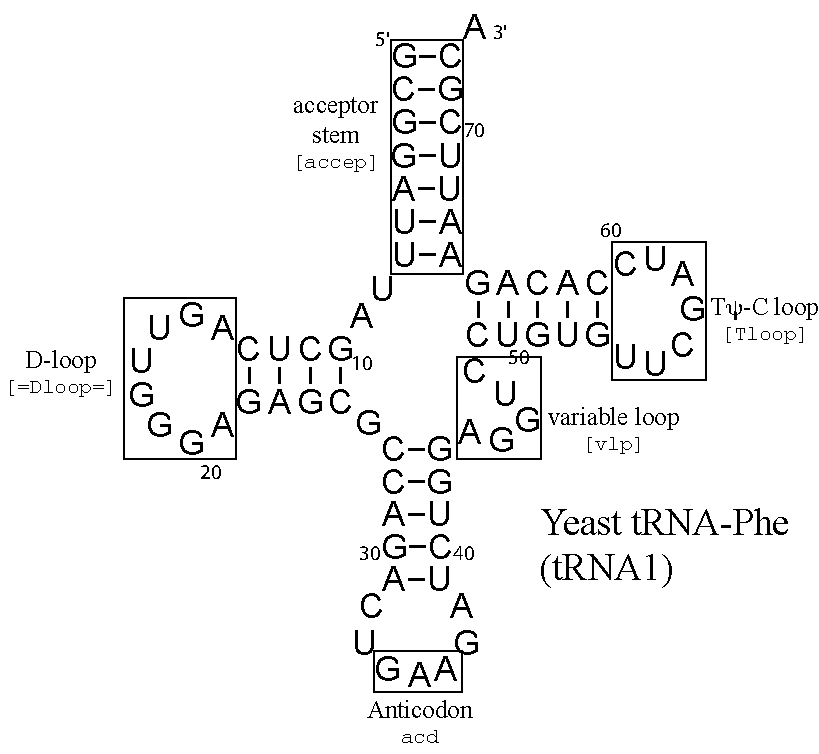
\includegraphics[scale=0.4]{Figures/trna1-DF6280-hand}
\end{minipage}
\vspace{1em}

This file is the same as \otext{tutorial/tRNA5.sto} except for the two
additional lines beginning with \otext{\#=GC RF}. This RF (reference)
annotation is required for using \otext{--hand}. When \otext{--hand}
is used, any non-gap character in the reference annotation will be
assigned as a match (consensus) position. Importantly, four different
characters are considered gaps: dashes (\otext{-}), underscores
(\otext{\_}), dots (\otext{.}) and tildes (\verb+~+). In this example
alignment, all columns are non-gap characters, so all columns will be
considered match positions.

Different regions of the secondary structure have been marked up using
abbreviations for the names of the regions in the reference
annotation. For example, \otext{acd} annotates the three positions of
the anticodon, and \otext{[vlp]} annotates the so-called variable
loop. I've used \otext{[} and \otext{]} to indicate region boundaries
in some cases. Crucially, I've avoided the use of any gap characters
for positions between named regions which I still want to be
considered match positions, and opted to use \otext{=} (which is not
considered a gap by \prog{cmbuild}) for these positions.

To build the hand-specified model from this alignment, do:

\user{cmbuild --hand tRNA5-hand.cm tutorial/tRNA5-hand.sto}
%tutorial regression: trna-hand-build.out

\begin{sreoutput}
# cmbuild :: covariance model construction from multiple sequence alignments
# INFERNAL 1.1 (October 2013)
# Copyright (C) 2013 Howard Hughes Medical Institute.
# Freely distributed under the GNU General Public License (GPLv3).
# - - - - - - - - - - - - - - - - - - - - - - - - - - - - - - - - - - - -
# CM file:                                            tRNA5-hand.cm
# alignment file:                                     ../../tutorial/tRNA5-hand.sto
# use #=GC RF annotation to define consensus columns: yes
# - - - - - - - - - - - - - - - - - - - - - - - - - - - - - - - - - - - -
#                                                                      rel entropy
#                                                                      -----------
# idx    name                     nseq eff_nseq   alen  clen  bps bifs    CM   HMM description
# ------ -------------------- -------- -------- ------ ----- ---- ---- ----- ----- -----------
       1 tRNA5-hand                  5     3.59     74    74   21    2 0.763 0.476 
#
# CPU time: 0.58u 0.00s 00:00:00.57 Elapsed: 00:00:00.60
\end{sreoutput}

The output reports that the model now has 74 match (consensus)
positions in the \otext{clen} column. If we had built this model
without specifying \otext{--hand} (as we did earlier in this tutorial)
the resulting model would have had only 72 consensus positions.
(I've annotated the two extra match positions with three gaps in
\otext{tRNA5.hand.sto} as match solely to demonstrate how
\otext{--hand} works, not because I think it's better to model these
positions as matches than inserts.)

Now, let's use this model to search the \emph{M. ruminantium} genome
again. First, the model must be calibrated. To save time, a calibrated
version of the file is in \otext{tutorial/tRNA5-hand.c.cm}. To do the
search:

\user{cmsearch tutorial/tRNA5-hand.c.cm tutorial/mrum-genome.fa}

The results are very similar to the earlier search with the
tRNA model built with default \prog{cmbuild} parameters (though not
identical since the model now has two additional match positions). The
important difference involves the hit alignments. Take a look at the
alignment for hit number 46 as an illustrative example:

\begin{widesreoutput}
>> NC_013790.1  Methanobrevibacter ruminantium M1 chromosome, complete genome
 rank     E-value  score  bias mdl mdl from   mdl to       seq from      seq to       acc trunc   gc
 ----   --------- ------ ----- --- -------- --------    ----------- -----------      ---- ----- ----
 (46) !   1.6e-09   43.2   0.0  cm        1       74 []      995344      995263 - .. 0.90    no 0.49

                                 v          v                                                            NC
                     (((((((,,<<<<________._>>>>,<<<<<_______>>>>>,,,........,,<<<<<_______>>>>>))))))): CS
   tRNA5-hand      1 gCcggcaUAGcgcAgUUGGuu.AgcgCgccagccUgucAagcuggAGg........UCCgggGUUCGAUUCcccGugccgGca 74    
                     :::G:CAUAGCG AG  GGU+ A CGCG:CAG:CU +++A:CUG: G+        UC:GGGGUUCGA UCCCC:UG:C:::A
  NC_013790.1 995344 AGAGACAUAGCGAAGC-GGUCaAACGCGGCAGACUCAAGAUCUGUUGAuuaguucuUCAGGGGUUCGAAUCCCCUUGUCUCUA 995263
                     ************9***.8886258***********************9444444445************************** PP
                     [accep]======[=Dloop=.]============acd=======[vl........p]=====[Tloop]=====[accep]= RF
\end{widesreoutput}

The reference annotation from the training alignment to \prog{cmbuild}
has been propagated to the hit as an extra \otext{RF} line at the
bottom of the alignment. All inserts in the alignment are annotated as
\otext{.} columns in the RF annotation. Note that the variable loop
(annotated as \otext{[vlp]} in the training alignment) contains 8
inserted residues. The RF annotation will also be transferred to
multiple alignments created with \prog{cmalign}.


\newpage

\section{The HMMER3 profile/sequence comparison pipeline}
\label{section:pipeline}
\setcounter{footnote}{0}

In this section, we briefly outline the processing pipeline for a
single profile/sequence comparison.\footnote{Code gurus and
  masochists: you can follow along in \ccode{src/p7\_pipeline.c}.} This
should help give you a sense of what HMMER3 is doing under the hood,
what sort of mistakes it may make (rarely, of course!), and what the
various results in the output actually mean.

In briefest outline, the comparison pipeline takes the following
steps:

\begin{description}
\item[\textbf{Null model.}] Calculate a score term for the ``null
  hypothesis'' (a probability model of \emph{non-}homology). This
  score correction is used to turn all subsequent profile/sequence bit
  scores into a final log-odds bit score.
  
\item[\textbf{MSV filter.}] The main acceleration heuristic. The MSV
  (``Multiple Segment Viterbi'') algorithm looks for one or more
  high-scoring \emph{ungapped} alignments. If the MSV score passes a
  set threshold, the entire sequence passes on to the next pipeline
  step; else it is rejected.

\item[\textbf{Bias filter.}] A hack that reduces false positive MSV
  hits due to biased composition sequences. A two-state HMM is
  constructed from the mean residue composition of the profile and the
  standard residue composition of the null model, and used to score
  the sequence. The MSV bit score is corrected using this as a second
  null hypothesis. If the MSV score still passes the MSV threshold,
  the sequence passes on to the next step; else it is rejected.  The
  bias filter score correction will also be applied to the Viterbi
  filter and Forward filter scores that follow.
  
\item[\textbf{Viterbi filter.}] A more stringent accelerated filter.
  An optimal (maximum likelihood) gapped alignment score is
  calculated. If this score passes a set threshold, the sequence
  passes to the next step; else it is rejected.

\item[\textbf{Forward filter/parser.}] The full likelihood of the
  profile/sequence comparison is evaluated, summed over the entire
  alignment ensemble, using the HMM Forward algorithm. This score is
  corrected to a bit score using the null model and bias filter
  scores. If the bit score passes a set threshold, the sequence passes
  on to the next step; else it is rejected.

\item[\textbf{Domain identification.}] Using the Forward parser
  results, now combined with a Backward parser, posterior
  probabilities of domain locations are calculated. A discrete set of
  putative domains (alignments) is identified by applying heuristics
  to posterior probabilities. This procedure identifies
  \emph{envelopes}: subsequences on the target sequence which contain
  a lot of probability mass for a match to the profile.

\item[\textbf{Alignment.}] For each identified domain, a full
  Forward/Backward algorithm is performed. An \emph{ad hoc} ``null2''
  hypothesis is constructed for each domain's composition and used to
  calculate a biased composition score correction. A maximum expected
  accuracy (MEA) alignment is calculated. This identifies one MEA
  alignment within each envelope.

\item[\textbf{Storage.}] Now we have a \emph{sequence score} (and
  P-value); the sequence contains one or more domains, each of which
  has a \emph{domain score} (and P-value), and each domain has an MEA
  alignment annotated with per-residue posterior probabilities.

\end{description}

In more detail, each step is described in subsections that follow:

\subsection{Null model.}

The ``null model'' calculates the probability that the target sequence
is \emph{not} homologous to the query profile. A HMMER bit score is
the log of the ratio of the sequence's probability according to the
profile (the homology hypothesis) over the null model probability (the
non-homology hypothesis). 

The null model is a one-state HMM configured to generate ``random''
sequences of the same mean length $L$ as the target sequence, with
each residue drawn from a background frequency distribution (a
standard i.i.d. model: residues are treated as independent and
identically distributed). Currently, this background frequency
distribution is hardcoded as the mean residue frequencies in Swiss-Prot
50.8 (October 2006).

For technical reasons, HMMER incorporates the \emph{residue emission}
probabilities of the null model directly into the profile, by turning
each emission probability in the profile into an odds ratio. The null
model score calculation therefore is only concerned with accounting
for the remaining \emph{transition} probabilities of the null model
and toting them up into a bit score correction.  The null model
calculation is fast, because it only depends on the length of the
target sequence, not its sequence.

\subsection{MSV filter.}

The sequence is aligned to the profile using a specialized model that
allows multiple high-scoring local ungapped segments to match.  The
optimal alignment score (Viterbi score) is calculated under this
multisegment model, hence the term MSV, for ``multi-segment
Viterbi''. This is HMMER's main speed heuristic.

The MSV score is comparable to BLAST's sum score (optimal sum of
ungapped alignment segments).  Roughly speaking, MSV is comparable to
skipping the heuristic word hit and hit extension steps of the BLAST
acceleration algorithm. HMMER uses vector parallelization methods to
accelerate optimal ungapped alignment.

The MSV score is a true log-odds likelihood ratio, so it obeys
conjectures about the expected score distribution \citep{Eddy08} that
allow immediate and accurate calculation of the statistical
significance (P-value) of the MSV bit score.

By default, comparisons with a P-value of $\leq$ 0.02 pass this
filter, meaning that about $2\%$ of nonhomologous sequences are
expected to pass. You can use the \ccode{--F1 <x>} option to change
this threshold. For example, \ccode{--F1 <0.05>} would pass 5\% of the
comparisons, making a search more sensitive but slower. Setting the
threshold to $>1.0$ (\ccode{--F1 99} for example) assures that all
comparisons will pass. Shutting off the MSV filter may be worthwhile
if you want to make sure you don't miss comparisons that have a lot of
scattered insertions and deletions. Alternatively, the \ccode{--max}
option causes the MSV filter step (and all other filter steps) to be
bypassed.

The MSV bit score is calculated as a log-odds score using the null
model for comparison. No correction for a biased composition or
repetitive sequence is done at this stage. For comparisons involving
biased sequences and/or profiles, more than 2\% of comparisons will
pass the MSV filter. At the end of search output, there is a line
like:

\begin{sreoutput}
 Passed MSV filter:                    107917  (0.020272); expected 106468.8 (0.02)
\end{sreoutput}

 which tells you how many and what fraction of comparisons passed the
 MSV filter, versus how many (and what fraction) were expected. 


\subsection{Biased composition filter.}

It's possible for profiles and/or sequences to have biased residue
compositions that result in ``significant'' log-odds bit scores not
because the profile matches the sequence particularly well, but
because the \emph{null model} matches the sequence particularly badly.

HMMER uses fairly good methods to compensate its scores for biased
composition, but these methods are computationally expensive and
applied late in the pipeline (described below).

In a few cases, profiles and/or target sequences are sufficiently
biased that too many comparisons pass the MSV filter, causing HMMER3
speed performance to be severely degraded. Although the final scores
and E-values at the end of the pipeline will be calculated taking into
account a ``null2'' model of biased composition and simple repetition,
the null2 model is dependent on a full alignment ensemble calculation
via the Forward/Backward algorithm, making it computationally complex,
so it won't get calculated until the very end. The treatment of biased
composition comparisons is probably the most serious problem remaining
in HMMER3. Solving it well will require more research. As a stopgap
solution to rescuing most of the speed degradation while not
sacrificing too much sensitivity, an \emph{ad hoc} biased composition
filtering step is applied to remove highly biased comparisons.

On the fly, a two-state HMM is constructed. One state emits residues
from the background frequency distribution (same as the null1 model),
and the other state emits residues from the mean residue composition
of the profile (i.e. the expected composition of sequences generated
by the core model, including match and insert states
[\ccode{p7\_hmm.c:p7\_hmm\_SetComposition()}]). Thus if the profile is
highly biased (cysteine-rich, for example; or highly hydrophobic with
many transmembrane segments), this composition bias will be captured
by this second state. This model's transitions are arbitrarily set
such that state 1 emits an expected length of 400 at a time, and state
2 emits an expected length of M/8 at a time (for a profile of length
M). An overall target sequence length distribution is set to a mean of
$L$, identical to the null1 model.

The sequence is then rescored using this ``bias filter model'' in
place of the null1 model, using the HMM Forward algorithm. (This
replaces the null1 model score at all subsequent filter steps in the
pipeline, until a final Forward score is calculated.) A new MSV bit
score is obtained.

If the P-value of this still satisfies the MSV thresholds, the
sequence passes the biased composition filter. 

The \ccode{--F1 <x>} option controls the P-value threshold for
passing the MSV filter score, both before (with the simple null1
model) and after the bias composition filter is applied.

The \ccode{--max} option bypasses all filters in the pipeline,
including the bias filter.

The \ccode{--nobias} option turns off (bypasses) the biased
composition filter.  The simple null model is used as a null
hypothesis for MSV and in subsequent filter steps. The biased
composition filter step compromises a small amount of sensitivity.
Though it is good to have it on by default, you may want to shut it
off if you know you will have no problem with biased composition hits.

 At the end of a search output, you will see a line like:

\begin{sreoutput}
 Passed bias filter:                   105665  (0.019849); expected 106468.8 (0.02)
\end{sreoutput}

which tells you how many and what fraction of comparisons passed the
biased composition filter, versus how many were expected. (If the
filter was turned off, all comparisons pass.)


\subsection{Viterbi filter.}

The sequence is now aligned to the profile using a fast Viterbi
algorithm for optimal gapped alignment.

This Viterbi implementation is specialized for speed.  It is
implemented in 8-way parallel SIMD vector instructions, using reduced
precision scores that have been scaled to 16-bit integers. Only one
row of the dynamic programming matrix is stored, so the routine only
recovers the score, not the optimal alignment itself. The reduced
representation has limited range; local alignment scores will not
underflow, but high scoring comparisons can overflow and return
infinity, in which case they automatically pass the filter.

The final Viterbi filter bit score is then computed using the
appropriate null model log likelihood (by default the biased
composition filter model score, or if the biased filter is off, just
the null model score). If the P-value of this score passes the Viterbi
filter threshold, the sequence passes on to the next step of the
pipeline.
 
The \ccode{--F2 <x>} option controls the P-value threshold for passing
the Viterbi filter score. The default is 0.001.
The \ccode{--max} option bypasses all filters in the pipeline.


At the end of a search output, you will see a line like:

\begin{sreoutput}
Passed Vit filter:                      2207  (0.00443803); expected 497.3 (0.001)
\end{sreoutput}

which tells you how many and what fraction of comparisons passed the
Viterbi filter, versus how many were expected.
 
  

\subsection{Forward filter/parser.}

The sequence is now aligned to the profile using the full Forward
algorithm, which calculates the likelihood of the target sequence
given the profile, summed over the ensemble of all possible
alignments.

This is a specialized time- and memory-efficient Forward
implementation called the ``Forward parser''. It is implemented in
4-way parallel SIMD vector instructions, in full precision (32-bit
floating point). It stores just enough information that, in
combination with the results of the Backward parser (below), posterior
probabilities of start and stop points of alignments (domains) can be
calculated in the domain definition step (below), although the
detailed alignments themselves cannot be.

The Forward filter bit score is calculated by correcting this score
using the appropriate null model log likelihood (by default the biased
composition filter model score, or if the biased filter is off, just
the null model score). If the P-value of this bit score passes the
Forward filter threshold, the sequence passes on to the next step of
the pipeline.

The bias filter score has no further effect in the pipeline. It is
only used in filter stages. It has \emph{no} effect on final reported
bit scores or P-values. Biased composition compensation for final bit
scores is done by a more complex domain-specific algorithm, described
below.

The \ccode{--F3 <x>} option controls the P-value threshold for passing
the Forward filter score. The default is 1e-5.  The \ccode{--max}
option bypasses all filters in the pipeline.

At the end of a search output, you will see a line like:

\begin{sreoutput}
Passed Fwd filter:                      1076  (0.00216371); expected 5.0 (1e-05)
\end{sreoutput}

which tells you how many and what fraction of comparisons passed the
Forward filter, versus how many were expected.


\subsection{Domain definition.}

A target sequence that reaches this point is very likely to contain
one or more significant matches to the profile. These matches are
referred to as ``domains'', since the main use of HMMER has
historically been to match profile HMMs from protein domain databases
like Pfam, and one of HMMER's strengths is to be able to cleanly parse
a multidomain target sequence into its multiple nonoverlapping hits to
the same domain model.

The domain definition step is essentially its own pipeline, with steps
as follows:\footnote{Code gurus and masochists can follow along in 
\ccode{src/p7\_domaindef.c}.}

\paragraph{Backward parser.}
The counterpart of the Forward parser algorithm is calculated in an
analogous time- and memory-efficient implementation. The Forward
algorithm gives the likelihood of all \emph{prefixes} of the target
sequence, summed over their alignment ensemble, and the Backward
algorithm gives the likelihood of all \emph{suffixes}. For any given
point of a possible model state/residue alignment, the product of the
Forward and Backward likelihoods gives the likelihood of the entire
alignment ensemble conditional on using that particular alignment
point. Thus, we can calculate things like the posterior probability
that an alignment starts or ends at a given position in the target
sequence.

\paragraph{Domain decoding.}
The posterior decoding algorithm is applied, to calculate the
posterior probability of alignment starts and ends (profile B and E
state alignments) with respect to target sequence position.

The sum of the posterior probabilities of alignment starts (B states)
over the entire target sequence is the \emph{expected number of
  domains} in the sequence.

In a tabular output (\ccode{--tblout}) file, this number is in the
column labeled \ccode{exp}.

\paragraph{Region identification.}

A heuristic is now applied to identify a \emph{non-overlapping} set of
``regions'' that contain significant probability mass suggesting the
presence of a match (alignment) to the profile.

For each region, the expected number of domains is calculated (again
by posterior decoding on the Forward/Backward parser results). This
number should be about 1: we expect each region to contain one local
alignment to the profile. 

In a tabular output (\ccode{--tblout}) file, the number of discrete
regions identified by this posterior decoding step is in the column
labeled \ccode{reg}. It ought to be almost the same as the expectation
\ccode{exp}. If it is not, there may be something funny going on, like
a tandem repetitive element in the target sequence (which can produce
so many overlapping weak hits that the sequence appears to be a
significant hit with lots of domains expected \emph{somewhere}, but
the probability is fuzzed out over the repetitive region and few or no
good discrete alignment regions can be identified).

\paragraph{Envelope identification.}

Now, within each region, we will attempt to identify \emph{envelopes}.
An \emph{envelope} is a subsequence of the target sequence that
appears to contain alignment probability mass for a likely domain (one
local alignment to the profile).

When the region contains $\simeq$1 expected domain, envelope
identification is already done: the region's start and end points are
converted directly to the envelope coordinates of a putative domain.

There are a few cases where the region appears to contain more than
one expected domain -- where more than one domain is closely spaced on
the target sequence and/or the domain scores are weak and the
probability masses are ill-resolved from each other. These
``multidomain regions'', when they occur, are passed off to an even
more \emph{ad hoc} resolution algorithm called \emph{stochastic
  traceback clustering}. In stochastic traceback clustering, we sample
many alignments from the posterior alignment ensemble, cluster those
alignments according to their overlap in start/end coordinates, and
pick clusters that sum up to sufficiently high probability. Consensus
start and end points are chosen for each cluster of sampled
alignments. These start/end points define envelopes.

These envelopes identified by stochastic traceback clustering are
\emph{not} guaranteed to be nonoverlapping. It's possible that there
are alternative ``solutions'' for parsing the sequence into domains,
when the correct parsing is ambiguous. HMMER will report all
high-likelihood solutions, not just a single nonoverlapping parse.

It's also possible (though rare) for stochastic clustering to identify
\emph{no} envelopes in the region.

In a tabular output (\ccode{--tblout}) file, the number of regions
that had to be subjected to stochastic traceback clustering is given
in the column labeled \ccode{clu}. This ought to be a small number
(often it's zero). The number of envelopes identified by stochastic
traceback clustering that overlap with other envelopes is in the
column labeled \ccode{ov}. If this number is non-zero, you need to be
careful when you interpret the details of alignments in the output,
because HMMER is going to be showing overlapping alternative
solutions. The total number of domain envelopes identified (either by
the simple method or by stochastic traceback clustering) is in the
column labeled \ccode{env}. It ought to be almost the same as the
expectation and the number of regions.

\paragraph{Maximum expected accuracy alignment.}
Each envelope is now aligned to the profile using the full
Forward/Backward algorithm. The profile is configured to ``unihit''
mode, so that the profile expects only one local alignment (domain) in
the envelope (as opposed to multiple domains).  Posterior decoding is
used to calculate the posterior probability of every detailed
alignment of profile state to sequence residue. The posterior
decodings are used to extract a ``maximum expected accuracy''
alignment. Each aligned residue is annotated with its posterior
probability in the Forward/Backward alignment ensemble.

Currently, the Forward, Backward, and posterior decoding calculations
at this step are \emph{not} memory efficient. They calculate matrices
requiring roughly $36 ML$ bytes, where $M$ is the profile length and
$L$ is the length of the envelope subsequence. Usually in
\prog{hmmsearch} and \prog{hmmscan}, profiles and envelopes are small
enough that this is not a problem. For example, a typical Pfam domain
model is about 200 residues long, matching to individual target
envelopes of about 200 residues each; this requires about 1.4 MB of
memory in MEA alignment. However, in the new \prog{phmmer} and
\prog{jackhmmer} programs, it's often going to be the case that you're
aligning an entire query sequence to an entire target sequence in a
single unresolved ``domain'' alignment. If this is titin (about 40,000
residues), it would require 57.6 GB of RAM. For this reason,
currently, \prog{phmmer} and \prog{jackhmmer} can only handle query
sequences of up to a few thousand residues. If you see a ``fatal
exception'' error complaining about failure of a large memory
allocation, you're almost certainly seeing a prohibitive memory
requirement at this stage.\footnote{We know how to fix this, with
  memory-efficient algorithms. It's just a matter of finding the time
  to do it.}

In a tabular output (\ccode{--tblout}) file, the number of domains in
envelopes (before any significance thresholding) is in the column
labeled \ccode{dom}. This will generally be the same as the number of
envelopes.

\paragraph{Biased composition score correction (``null2'')}
An \emph{ad hoc} biased composition score correction is calculated for
each envelope, using the posterior decoding. A corrected bit score and
P-value for each envelope is calculated. These per-domain scores and
P-values will eventually be subjected to per-domain thresholds to
define significant domains that will appear in output.

Once the position-specific ``null2'' score is available, specifying a
biased composition correction that applies to every residue, the total
corrected bit score for the target sequence is recalculated, by
summing up envelope scores for each significant domain.






\newpage
\section{Profile SCFG construction: the \texttt{cmbuild} program}
\label{section:cmbuild}
\setcounter{footnote}{0}

Infernal builds a model of consensus RNA secondary
structure using a formalism called a \emph{covariance model} (CM),
which is a type of \emph{profile stochastic context-free grammar}
(profile SCFG) \citep{Eddy94,Durbin98,Eddy02b}.

What follows is a technical description of what a CM is, how it
corresponds to a known RNA secondary structure, and how it is built
and parameterized.\footnote{Much of this text is taken from
\citep{Eddy02b}.}  You certainly don't have to understand the technical
details of CMs to understand \prog{cmbuild} or Infernal,
but it will probably help to at least skim this part. After that is a
description of what the \prog{cmbuild} program does to build a CM from
an input RNA multiple alignment, and how to control the behavior of
the program.

\subsection{Technical description of a covariance model}

\subsubsection{Definition of a stochastic context free grammar}

A stochastic context free grammar (SCFG) consists of the following:

\begin{itemize}
\item $M$ different nonterminals (here called \emph{states}). I will use capital
      letters to refer to specific nonterminals; $V$ and $Y$ will be used
      to refer generically to unspecified nonterminals.
\item $K$ different terminal symbols (e.g. the observable alphabet,
      {a,c,g,u} for RNA). I will use small letters $a,b$ to refer
      generically to terminal symbols.
\item a number of \emph{production rules} of the form: $V \rightarrow
\gamma$, where $\gamma$ can be any string of nonterminal and/or
terminal symbols, including (as a special case) the empty string
$\epsilon$.
\item Each production rule is associated with a probability, such that
      the sum of the production probabilities for any given
      nonterminal $V$ is equal to 1.
\end{itemize} 

\subsubsection{SCFG productions allowed in CMs}

A CM is a specific, repetitive SCFG architecture consisting of groups
of model states that are associated with base pairs and
single-stranded positions in an RNA secondary structure consensus. A
CM has seven types of states and production rules:

\vspace{0.5em}
\begin{center}
\begin{tabular}{lllll}
State type & Description             &  Production             & Emission & Transition\\ \hline
P & (pair emitting)   & $P \rightarrow a Y b$ & $e_v(a,b)$ & $t_v(Y)$  \\
L & (left emitting)   & $L \rightarrow a Y$   & $e_v(a)$   & $t_v(Y)$  \\
R & (right emitting)  & $R \rightarrow Y a$   & $e_v(a)$   & $t_v(Y)$  \\
B & (bifurcation)     & $B \rightarrow S S$   & 1     &     1     \\
D & (delete)          & $D \rightarrow Y$     & 1     &   $t_v(Y)$  \\
S & (start)           & $S \rightarrow Y$     &    1     & $t_v(Y)$  \\
E & (end)             & $E \rightarrow \epsilon$ & 1     &     1     \\
\end{tabular}
\end{center}
\vspace{0.5em}

Each overall production probability is the independent product of an
emission probability $e_v$ and a transition probability $t_v$, both of
which are position-dependent parameters that depend on the state $v$
(analogous to hidden Markov models). For example, a particular pair
(P) state $v$ produces two correlated letters $a$ and $b$ (e.g. one of
16 possible base pairs) with probability $e_v(a,b)$ and transits to
one of several possible new states $Y$ of various types with
probability $t_v(Y)$.  A bifurcation (B) state splits into two new
start ($S$) states with probability 1.  The E state is a special case
$\epsilon$ production that terminates a derivation.

A CM consists of many states of these seven basic types, each with its
own emission and transition probability distributions, and its own set
of states that it can transition to. Consensus base pairs will be
modeled by P states, consensus single stranded residues by L and R
states, insertions relative to the consensus by more L and R states,
deletions relative to consensus by D states, and the branching
topology of the RNA secondary structure by B, S, and E states. The
procedure for starting from an input multiple alignment and
determining how many states, what types of states, and how they are
interconnected by transition probabilities is described next.

\subsubsection{From consensus structural alignment to guide tree}

Figure~\ref{fig:input_alignment} shows an example input file: a
multiple sequence alignment of homologous RNAs, with a line in WUSS
notation that describes the consensus RNA secondary structure. The
first step of building a CM is to produce a binary \emph{guide tree}
of \emph{nodes} representing the consensus secondary structure. The
guide tree is a parse tree for the consensus structure, with nodes as
nonterminals and alignment columns as terminals.

\begin{figure}[t]
\begin{center}
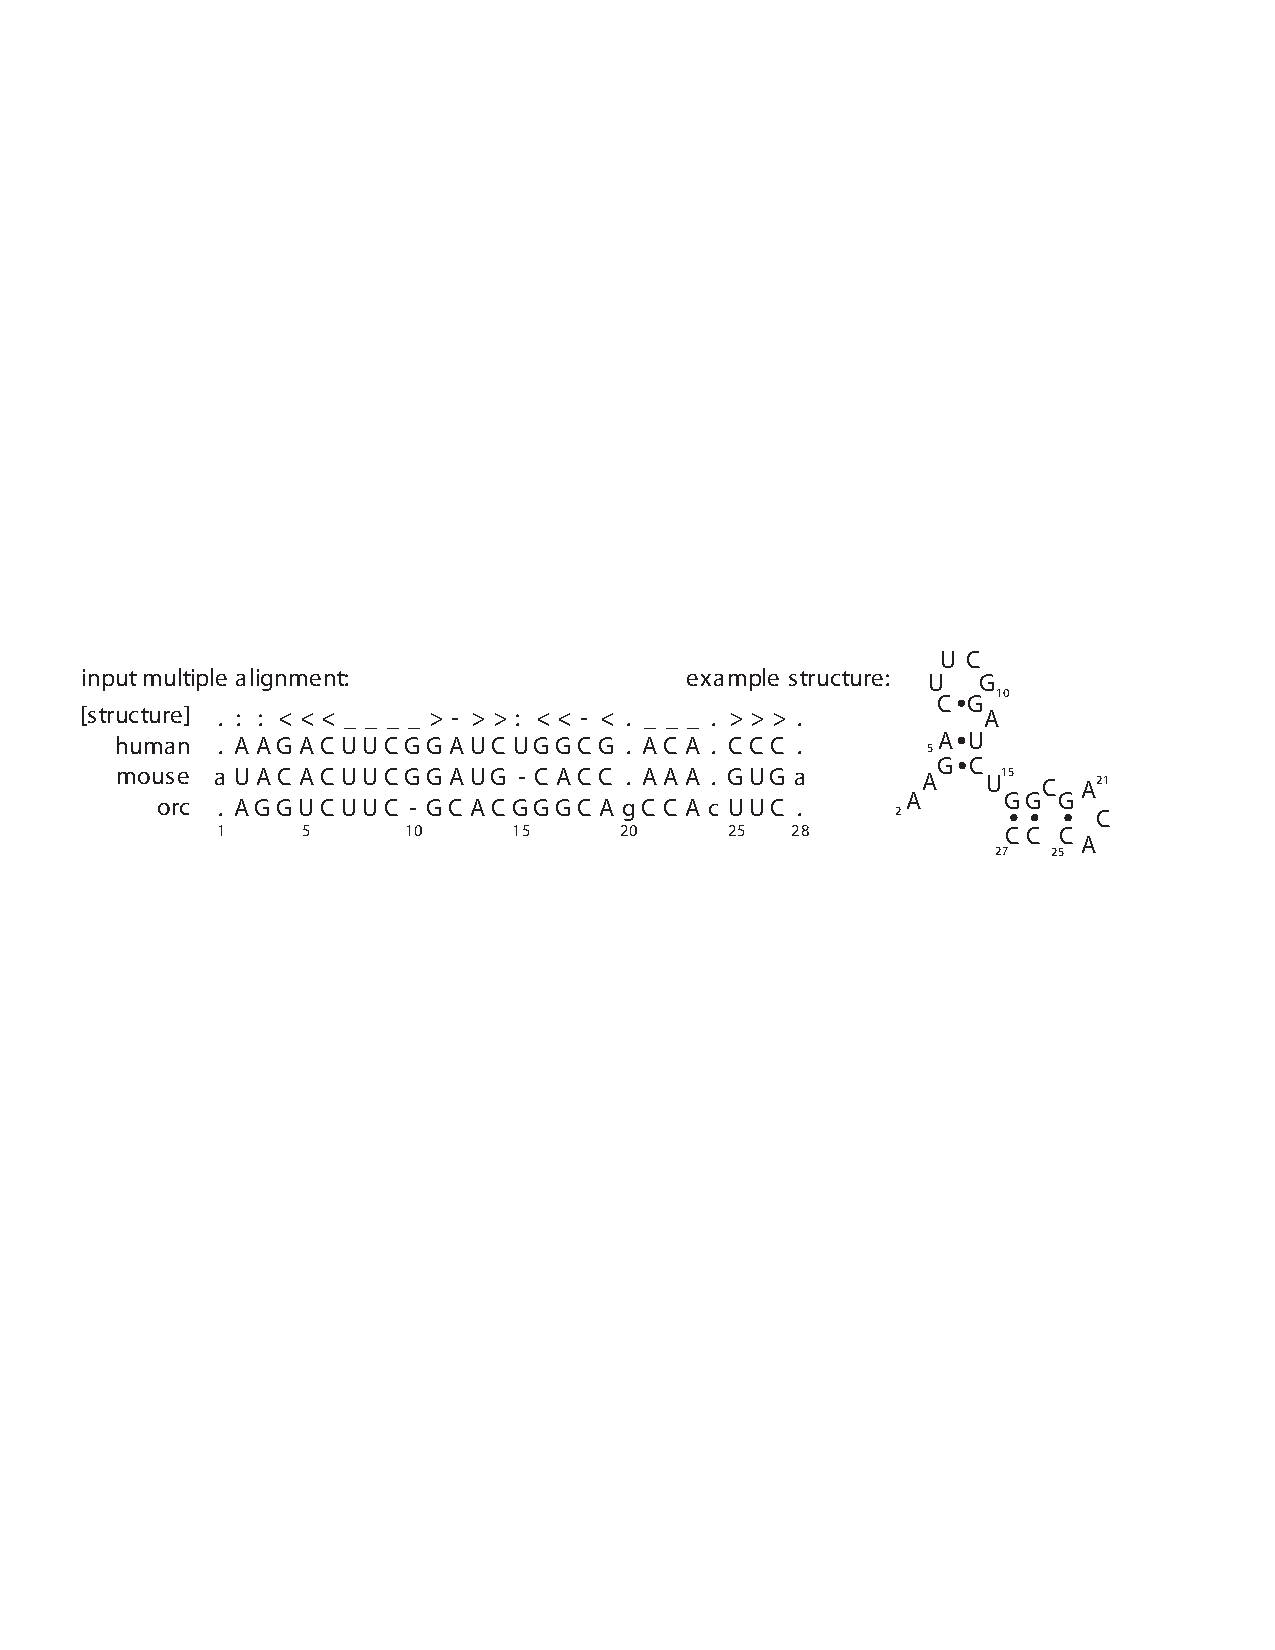
\includegraphics[scale=0.8]{Figures/input_alignment}
\end{center}
\caption{\small\textbf{An example RNA sequence family.} Left: a toy multiple
alignment of three sequences, with 28 total columns, 24 of which will
be modeled as consensus positions. The [structure] line annotates the
consensus secondary structure in WUSS notation.
Right: the secondary structure of the ``human'' sequence.} 
\label{fig:input_alignment}
\end{figure}

The guide tree has eight types of nodes:

\vspace{0.5em}
\begin{center}
\begin{tabular}{lll}
Node      & Description        &  Main state type          \\ \hline
MATP  & (pair)                 & P \\
MATL  & (single strand, left)  & L \\
MATR  & (single strand, right) & R \\
BIF   & (bifurcation)          & B \\
ROOT  & (root)                 & S \\
BEGL  & (begin, left)          & S \\
BEGR  & (begin, right)         & S \\
END   & (end)                  & E \\
\end{tabular}
\end{center}
\vspace{0.5em}
 
These consensus node types correspond closely with the CM's final
state types. Each node will eventually contain one or more states. The
guide tree deals with the consensus structure. For individual
sequences, we will need to deal with insertions and deletions with
respect to this consensus. The guide tree is the skeleton on which we
will organize the CM. For example, a MATP node will contain a P-type
state to model a consensus base pair; but it will also contain several
other states to model infrequent insertions and deletions at or
adjacent to this pair.

The input alignment is first used to construct a consensus secondary
structure (Figure~\ref{fig:cm_nodetree}) that defines which aligned
columns will be ignored as non-consensus (and later modeled as
insertions relative to the consensus), and which consensus alignment
columns are base-paired to each other. For the purposes of this
description, I assume that both the structural annotation and the
labeling of insert versus consensus columns is given in the input
file, as shown in the alignment in Figure~\ref{fig:input_alignment},
where both are are indicated by the WUSS notation in the [structure]
line (where, e.g., insert columns are marked with \otext{.}). (In
practice, \prog{cmbuild} does need secondary structure annotation, but
it doesn't require insert/consensus annotation or full WUSS notation
in its input alignment files; this would require a lot of manual
annotation.  More on this later.)

\begin{figure}[t]
\begin{center}
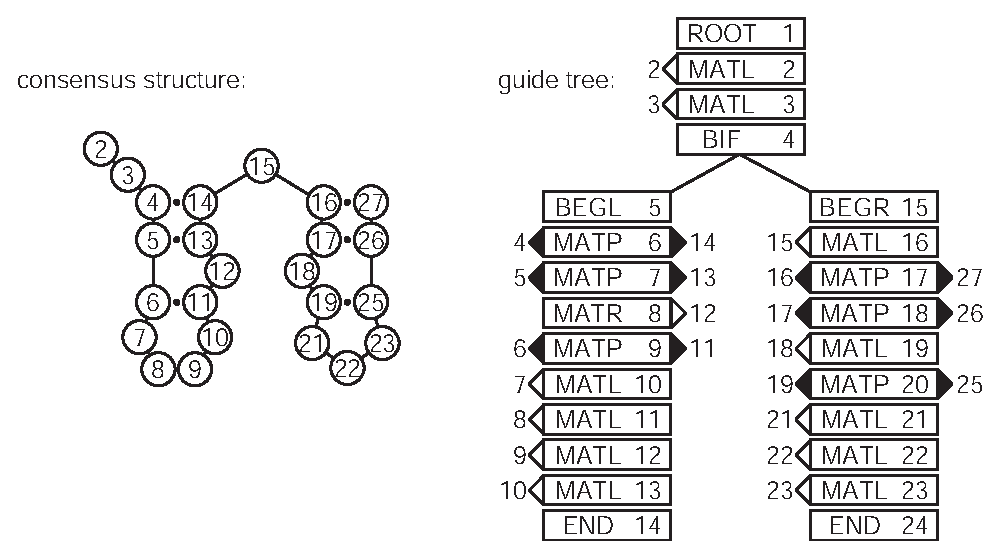
\includegraphics[width=5in]{Figures/cm_nodetree}
\end{center}
\caption{\small\textbf{The structural alignment is converted to a guide
tree.} Left: the consensus secondary structure is derived from the
annotated alignment in Figure~\ref{fig:input_alignment}. Numbers in
the circles indicate alignment column coordinates: e.g.  column 4 base
pairs with column 14, and so on. Right: the CM guide tree
corresponding to this consensus structure. The nodes of the tree are
numbered 1..24 in preorder traversal (see text). MATP, MATL, and MATR
nodes are associated with the columns they generate: e.g., node 6 is a
MATP (pair) node that is associated with the base-paired columns 4 and
14.}
\label{fig:cm_nodetree}
\end{figure}

Given the consensus structure, consensus base pairs are assigned to
MATP nodes and consensus unpaired columns are assigned to MATL or MATR
nodes. One ROOT node is used at the head of the tree.  Multifurcation
loops and/or multiple stems are dealt with by assigning one or more
BIF nodes that branch to subtrees starting with BEGL or BEGR head
nodes. (ROOT, BEGL, and BEGR start nodes are labeled differently
because they will be expanded to different groups of states; this has
to do with avoiding ambiguous parse trees for individual sequences, as
described below.) Alignment columns that are considered to be
insertions relative to the consensus structure are ignored at this
stage.

In general there will be more than one possible guide tree for any
given consensus structure. Almost all of this ambiguity is eliminated
by three conventions: (1) MATL nodes are always used instead of MATR
nodes where possible, for instance in hairpin loops; (2) in describing
interior loops, MATL nodes are used before MATR nodes; and (3) BIF
nodes are only invoked where necessary to explain branching secondary
structure stems (as opposed to unnecessarily bifurcating in single
stranded sequence). One source of ambiguity remains. In invoking a
bifurcation to explain alignment columns $i..j$ by two substructures
on columns $i..k$ and $k+1..j$, there will be more than one possible
choice of $k$ if $i..j$ is a multifurcation loop containing three or
more stems. The choice of $k$ impacts the performance of the divide
and conquer algorithm; for optimal time performance, we will want
bifurcations to split into roughly equal sized alignment problems, so
I choose the $k$ that makes $i..k$ and $k+1..j$ as close to the same
length as possible.

The result of this procedure is the guide tree. The nodes of the guide
tree are numbered in preorder traversal (e.g. a recursion of ``number
the current node, visit its left child, visit its right child'': thus
parent nodes always have lower indices than their children). The guide
tree corresponding to the input multiple alignment in
Figure~\ref{fig:input_alignment} is shown in
Figure~\ref{fig:cm_nodetree}.

\subsubsection{From guide tree to covariance model}

A CM must deal with insertions and deletions in individual sequences
relative to the consensus structure. For example, for a consensus base
pair, either partner may be deleted leaving a single unpaired residue,
or the pair may be entirely deleted; additionally, there may be
inserted nonconsensus residues between this pair and the next pair in
the stem. Accordingly, each node in the master tree is expanded into
one or more \emph{states} in the CM as follows:

\vspace{0.5em}
\begin{center}
\begin{tabular}{llccc}
       &                     & total \#& \# of split& \# of insert\\
Node   &  States             & states  & states     & states \\ \hline
MATP   & [MP ML MR D] IL IR  &   6     &   4        &  2   \\
MATL   & [ML D] IL           &   3     &   2    &  1   \\
MATR   & [MR D] IR           &   3     &   2    &  1   \\
BIF    & [B]                 &   1     &   1    &  0   \\
ROOT   & [S] IL IR           &   3     &   1    &  2   \\
BEGL   & [S]                 &   1     &   1    &  0   \\
BEGR   & [S] IL              &   2     &   1    &  1   \\
END    & [E]                 &   1     &   1    &  0   \\ \hline
\end{tabular}
\end{center}
\vspace{0.5em}

Here we distinguish between consensus (``M'', for ``match'') states
and insert (``I'') states. ML and IL, for example, are both L type
states with L type productions, but they will have slightly different
properties, as described below.

The states are grouped into a \emph{split set} of 1-4 states (shown in
brackets above) and an \emph{insert set} of 0-2 insert states. The
split set includes the main consensus state, which by convention is
first. One and only one of the states in the split set must be visited
in every parse tree (and this fact will be exploited by the divide and
conquer algorithm). The insert state(s) are not obligately visited,
and they have self-transitions, so they will be visited zero or more
times in any given parse tree.

State transitions are then assigned as follows. For bifurcation nodes,
the B state makes obligate transitions to the S states of the child
BEGL and BEGR nodes. For other nodes, each state in a split set has a
possible transition to every insert state in the \emph{same} node, and
to every state in the split set of the \emph{next} node. An IL state
makes a transition to itself, to the IR state in the same node (if
present), and to every state in the split set of the next node. An IR
state makes a transition to itself and to every state in the split set
of the next node.

There is one exception to this arrangement of transitions: insert
states that are immediately before an END node are effectively
\emph{detached} from the model by making transitions into them
impossible. This inelegant solution was imposed on the CM model
building procedure to fix a design flaw that allowed an ambiguity in
the determination of a parsetree given a structure. The detachment of
these special insert states removes this ambiguity.

This arrangement of transitions guarantees that (given the guide tree)
there is unambiguously one and only one parse tree for any given
individual structure. This is important. The algorithm will find a
maximum likelihood parse tree for a given sequence, and we wish to
interpret this result as a maximum likelihood structure, so there must
be a one to one relationship between parse trees and secondary
structures \citep{Giegerich00}.

The final CM is an array of $M$ states, connected as a directed graph
by transitions $t_v(y)$ (or probability 1 transitions $v \rightarrow
(y,z)$ for bifurcations) with the states numbered such that $(y,z)
\geq v$. There are no cycles in the directed graph other than cycles
of length one (e.g. the self-transitions of the insert states). We can
think of the CM as an array of states in which all transition
dependencies run in one direction; we can do an iterative dynamic
programming calculation through the model states starting with the
last numbered end state $M$ and ending in the root state $1$.  An
example CM, corresponding to the input alignment of
Figure~\ref{fig:input_alignment}, is shown in
Figure~\ref{fig:cm_graph}.

As a convenient side effect of the construction procedure, it is
guaranteed that the transitions from any state are to a
\emph{contiguous} set of child states, so the transitions for state
$v$ may be kept as an offset and a count. For example, in
Figure~\ref{fig:cm_graph}, state 12 (an MP) connects to states 16, 17,
18, 19, 20, and 21. We can store this as an offset of 4 to the first
connected state, and a total count of 6 connected states.  We know
that the offset is the distance to the next non-split state in the
current node; we also know that the count is equal to the number of
insert states in the current node, plus the number of split set states
in the next node. These properties make establishing the connectivity
of the CM trivial. Similarly, all the parents of any given state are
also contiguously numbered, and can be determined analogously. We are
also guaranteed that the states in a split set are numbered
contiguously.  This contiguity is exploited by the divide and conquer
implementation.

\begin{figure}[tp]
\begin{center}
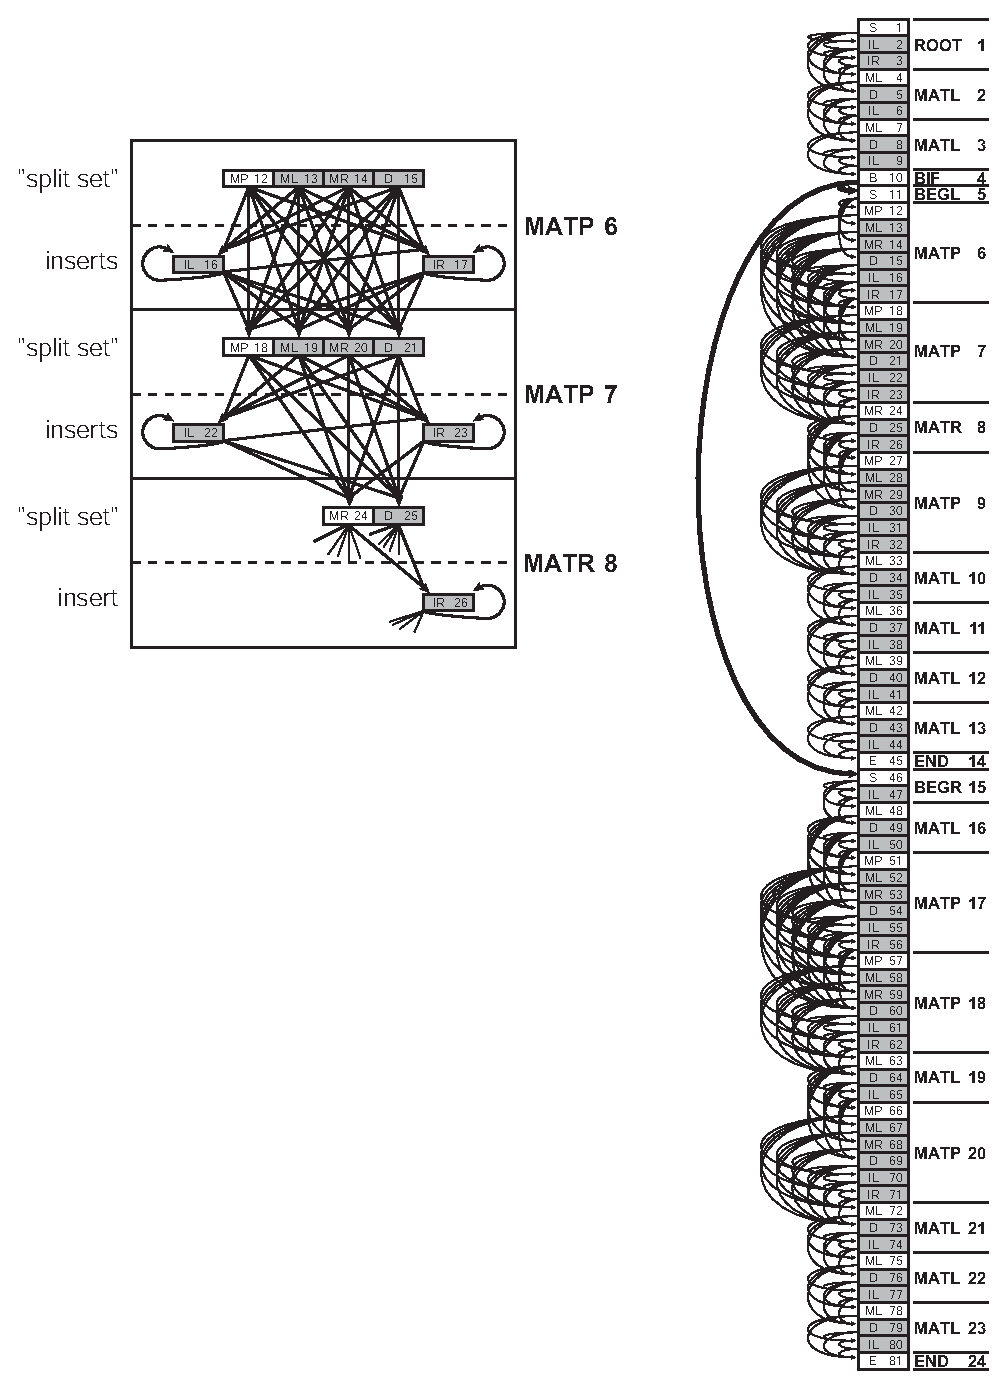
\includegraphics[width=5in]{Figures/cm_graph}
\end{center}
\caption{\small\textbf{A complete covariance model.} Right: the CM
corresponding to the alignment in Figure~\ref{fig:input_alignment}.
The model has 81 states (boxes, stacked in a vertical array). Each
state is associated with one of the 24 nodes of the guide tree (text
to the right of the state array). States corresponding to the
consensus are in white. States responsible for insertions and
deletions are gray. The transitions from bifurcation state B10 to
start states S11 and S46 are in bold because they are special: they
are an obligate (probability 1) bifurcation. All other transitions
(thin arrows) are associated with transition probabilities.  Emission
probability distributions are not represented in the figure. Left: the
states are also arranged according to the guide tree. A blow up of
part of the model corresponding to nodes 6, 7, and 8 shows
more clearly the logic of the connectivity of transition probabilities
(see main text), and also shows why any parse tree must transit through
one and only one state in each ``split set''.}
\label{fig:cm_graph}
\end{figure}

\subsubsection{Parameterization}

Using the guide tree and the final CM, each individual sequence in the
input multiple alignment can be converted unambiguously to a CM parse
tree, as shown in Figure~\ref{fig:parsetrees}. Weighted counts for
observed state transitions and singlet/pair emissions are then
collected from these parse trees. These counts are converted to
transition and emission probabilities, as maximum \emph{a posteriori}
estimates using mixture Dirichlet priors
\citep{Sjolander96,Durbin98,NawrockiEddy07}. 

\begin{figure}[t]
\begin{center}
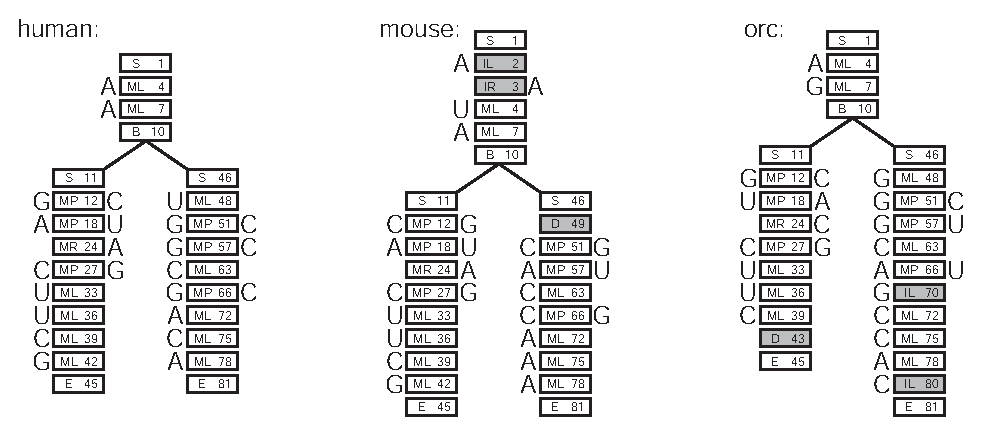
\includegraphics[width=5in]{Figures/parsetrees}
\end{center}
\caption{\small\textbf{Example parse trees.} Parse trees are shown for the
three sequences/structures from Figure~\ref{fig:input_alignment},
given the CM in Figure~\ref{fig:cm_graph}. For each sequence, each
residue must be associated with a state in the parse tree. (The
sequences can be read off its parse tree by starting at the upper left
and reading counterclockwise around the edge of parse tree.) Each
parse tree corresponds directly to a secondary structure -- base pairs
are pairs of residues aligned to MP states. A collection of parse
trees also corresponds to a multiple alignment, by aligning residues
that are associated with the same state -- for example, all three
trees have a residue aligned to state ML4, so these three residues
would be aligned together. Insertions and deletions relative to the
consensus use nonconsensus states, shown in gray.}
\label{fig:parsetrees}
\end{figure}

\subsubsection{Comparison to profile HMMs}

The relationship between an SCFG and a covariance model is analogous
to the relationship of hidden Markov models (HMMs) and profile HMMs
for modeling multiple sequence alignments
\citep{Krogh94,Durbin98,Eddy98}. A comparison may be instructive to
readers familiar with profile HMMs.  A profile HMM is a repetitive HMM
architecture that associates each consensus column of a multiple
alignment with a single type of model node -- a MATL node, in the
above notation. Each node contains a ``match'', ``delete'', and
``insert'' HMM state -- ML, IL, and D states, in the above notation.
The profile HMM also has special begin and end states. Profile HMMs
could therefore be thought of as a special case of CMs. An
unstructured RNA multiple alignment would be modeled by a guide tree
of all MATL nodes, and converted to an unbifurcated CM that would
essentially be identical to a profile HMM. (The only difference is
trivial; the CM root node includes a IR state, whereas the start node
of a profile HMM does not.) All the other node types (especially MATP,
MATR, and BIF) and state types (e.g. MP, MR, IR, and B) are SCFG
augmentations necessary to extend profile HMMs to deal with RNA
secondary structure.


\subsection{The \prog{cmbuild} program, step by step}
%\addtocontents{faq}{\textbf{Questions about using cmbuild:}}

The \prog{cmbuild} command line syntax is:

\user{cmbuild <options> [cmfile] [alifile]}

where \prog{[alifile]} is the name of the input alignment file, and
\prog{[cmfile]} is the name of the output CM file. What follows
describes the steps that \prog{cmbuild} goes through, and the most
important options that can be chosen to affect its behavior.

\subsubsection{Alignment input file}

The input alignment file must be in Stockholm format, and it must have
a consensus secondary structure annotation line (\otext{\#=GC SS\_cons}).

The program is actually capable of reading many common multiple
alignment formats (ClustalW, PHYLIP, GCG MSF, and others) but no other
format currently supports consensus RNA secondary structure
annotation. This may change in the future, either when other formats
allow structure annotation, or when \prog{cmbuild} is capable of
inferring consensus structure from the alignment by automated
comparative analysis, as the earlier COVE suite was capable
of \citep{Eddy94}. 

If the file does not exist, is not readable, or is not in a recognized
format, the program exits with a ``Alignment file doesn't exist or is
not readable'' error. If the file does not have consensus secondary
structure annotation, the program exits with a ``no consensus
structure annotation'' error. This includes all non-Stockholm
alignment files.

% EPN, Wed Apr  2 12:47:54 2008, the cat my.sto | cmbuild command
% in this faq no longer works.
\begin{srefaq}{Why does \prog{cmbuild} have a \prog{--informat} option, if it only
accepts Stockholm?} If you don't specify \prog{--informat}, the
software has to autodetect the file format. Autodetection of file
formats doesn't work in certain advanced/nonstandard cases, for
instance if you're reading the alignment from standard input instead
of from a file. The \prog{--informat} allows you to override
autodetection; e.g. \prog{cat my.sto | cmbuild --informat Stockholm
my.cm -} is an example of reading the alignment from piped standard
input.
\end{srefaq}

\subsubsection{Parsing secondary structure annotation}

The structure annotation line only needs to indicate which columns are
base paired to which. It does not have to be in full WUSS notation.
Even if it is, the details of the notation are largely ignored.
Nested pairs of \otext{<>}, \otext{()}, \otext{[]}, or \otext{{}} symbols
are interpreted as base paired columns. All other columns marked with
the symbols \otext{:,\_-.~} are interpreted as single stranded columns.

A simple minimal annotation is therefore to use \otext{<>} symbols to
mark base pairs and \otext{.} for single stranded columns.

If a secondary structure annotation line is in WUSS notation and it
contains valid pseudoknot annotation (e.g.\ additional non-nested
stems marked with AAA,aaa or BBB,bbb, etc.), this annotation is
ignored because Infernal cannot handle
pseudoknots. Internally, these columns are treated as if they were
marked with \otext{.} symbols.

\begin{srefaq}{How should I choose to annotate pseudoknots?} 
Infernal can only deal with nested base pairs. If there is
a pseudoknot, you have to make a choice of which stem to annotate as
normal nested structure (thus including it in the model) and which
stem to call additional ``pseudoknotted'' structure (thus ignoring it
in the model). For example, for a simple two-stem pseudoknot, should
you annotate it as \otext{AAAA.<<<<aaaa....>>>>}, or
\otext{<<<<.AAAA>>>>....aaaa}?  From an RNA structure viewpoint, which
stem I label as the pseudoknotted one is an arbitrary choice; but
since one of the stems in the pseudoknot will have to be modeled as a
single stranded region by Infernal, the choice makes a
slight difference in the performance of your model. You want your
model to capture as much information content as possible.  Thus, since
the information content of the model is a sum of the sequence
conservation plus the additional information contributed by pairwise
correlations in base-paired positions, you should tend to annotate the
shorter stem as the ``pseudoknot'' (modeling as many base pairs as
possible), and you should also annotate the stem with the more
conserved primary sequence as the ``pseudoknot'' (if one stem is more
conserved at the sequence level, you won't lose as much by modeling
that one as primary sequence consensus only).
\end{srefaq}

If (aside from any ignored pseudoknot annotation) the structure
annotation line contains characters other than \otext{<>()[]{}:\_-,.~}
then those characters are ignored (treated as \otext{.}) and a warning
is printed.

If, after this ``data cleaning'', the structure annotation is
inconsistent with a secondary structure (for example, if the number of
\otext{<} and \otext{>} characters isn't the same), then the program
exits with a ``failed to parse consensus structure annotation'' error.

\subsubsection{Sequence weighting}

By default, the input sequences are weighted in two ways to compensate
for biased sampling (phylogenetic correlations).  Relative sequence
weights are calculated by the Henikoff position-based method.
\citep{Henikoff94b}.  (The \prog{--wpb} option forces position-based
weights, but is redundant since that's the default.)  To turn relative
weighting off (e.g. set all weights to 1.0), use the \prog{--wnone}
option.

Some alignment file formats allow relative sequence weights to be
given in the file. This includes Stockholm format, which has
\otext{\#=GS WT} weight annotations. Normally \prog{cmbuild} ignores any
such input weights.  The \prog{--wgiven} option tells \prog{cmbuild}
to use them.  This lets you set the weights with any external
procedure you like; for example, the \prog{esl-weight} utility program in
Easel\footnote{This program will be in
  \ccode{infernal/easel/miniapps/} after building Infernal.} 
implements some common weighting algorithms,
including the Gerstein/Sonnhammer/Chothia weighting scheme
\citep{Gerstein94}.

Absolute weights (the ``effective sequence number'') is calculate by
``entropy weighting'' \citep{Karplus98}. This sets the balance between
the prior and the data, and affects the information content of the
model. Entropy weighting reduces the effective sequence number (the
total sum of the weights) and increases the entropy (degrading the
information content) of the model until a threshold is reached. The
default entropy is 1.41 bits per position (roughly 0.59 bits of
information, relative to uniform base composition). This threshold can
be changed with the \prog{--ere <x>} option. Entropy weighting may
be turned off entirely with the \prog{--enone} option.


\subsubsection{Architecture construction}

The CM architecture is now constructed from your input alignment and
your secondary structure annotation, as described in the previous
section. 

The program needs to determine which columns are consensus (match)
columns, and which are insert columns. (Remember that although WUSS
notation allows insertions to be annotated in the secondary structure
line, \prog{cmbuild} is only paying attention to annotated base
pairs.) By default, it does this by a simple rule based on the
frequency of residues (non-gaps) in a column. If the frequency of
residues is lower than a threshold, the column is considered to be
an insertion. Importantly though this frequency is determined using
the relative weights from the sequence weighting step, instead of
absolute gaps (e.g. a residue in a sequence with weight $0.8$ will count
as $0.8$ residues)\footnote{This behavior is new in Infernal 1.1, in all
previous versions of Infernal, absolute weights, not relative weights
were used at this step.}.

The threshold defaults to 0.5. It can be changed to another number
\otext{<x>} (from 0 to 1.0) by the \prog{--symfrac <x>} option.  The
lower the number, the more columns are included in the model.  At
\prog{--symfrac 0.0}, all the columns are considered to be part of
the consensus. At \prog{--symfrac 1.0}, only columns with no gaps are.

You can also manually specify which columns are consensus versus
insert by including reference coordinate annotation (e.g. a
\otext{\#=GC RF} line, in Stockholm format) and using the
\prog{--hand} option. There's an example of this in the tutorial. Any
columns marked by non-gap symbols become consensus columns. (The
simplest thing to do is mark consensus columns with x's, and insert
columns with \otext{.}'s. Remember that spaces aren't allowed in
alignments in Stockholm format.) If you set the \prog{--hand} option but
your file doesn't have reference coordinate annotation, the program
exits with an error.

\subsubsection{Parameterization}

Weighted observed emission and transition counts are then collected
from the alignment data. These count vectors $c$ are then converted to
estimated probabilities $p$ using mixture Dirichlet priors
\citep{Sjolander96, Durbin98, NawrockiEddy07}. You can provide your
own prior as a file, using the \prog{--prior <f>} option.

As an exception, insert state emission probabilities are not learned
from the counts from implicit parse trees of sequences in the input
alignment, instead they are all set to 0.25 for each of the four RNA
nucleotides.  Another exception is made for transition counts in
ROOT\_IL and ROOT\_IR states from the implicit parsetrees. Any
transition counts in these states are \emph{ignored} by the
construction procedure -- they are set to zero before the transition
probability parameters for these states are determined.

\subsubsection{Naming the model}

Each CM gets a name. Stockholm format allows the alignment to have a
name, provided in the \otext{\#=GF ID} tag. If this name is provided,
it is used as the CM name.

Stockholm format allows more than one alignment per file, and
\prog{cmbuild} supports this: CM files can contain more than one
model, and if you say e.g.\ \prog{cmbuild Rfam.cm Rfam.sto} where
\otext{Rfam.sto} contains a whole database of alignments,
\prog{cmbuild} will create a database of CMs in the \prog{Rfam.cm} file,
one per alignment. 

If a name is not provided in the Stockholm \otext{\#=GF ID}
annotation, the name given to each CM is the input filename. This will
not work if the alignment file has more than one alignment. In that
case, you must include names for each alignment.

If the alignment file only has 1 alignment in it, you can override the
automatic naming conventions and provide your own name with the \prog{-n <s>}
option, where \prog{<s>} is any string. 

\subsubsection{Saving the model}

The model is now saved to a file, according to the filename specified
on the command line. By default, a new file is created, and the model
is saved in a portable ASCII text format. This format is described in
section~\ref{section:formats} of this guide.

If the cmfile already exists, the program exits with an error. The
\prog{-F} option causes the new model to overwrite an existing
cmfile. 



\newpage
\section{Tabular output formats}
\label{section:tabular}
\setcounter{footnote}{0}

\subsection{The target hits table}

The \ccode{--tblout} output option in \prog{cmscan} and
  \prog{cmsearch} produces the \emph{target hits table}.  The target
  hits table consists of one line for each different query/target
  comparison that met the reporting thresholds, ranked by decreasing
  statistical significance (increasing E-value).  Each line consists
  of \textbf{18 space-delimited fields} followed by a free text target
  sequence description, as follows:\footnote{The \ccode{tblout} format
  is deliberately space-delimited (rather than tab-delimited) and
  justified into aligned columns, so these files are suitable both for
  automated parsing and for human examination. Tab-delimited data
  files are difficult for humans to examine and spot check. For this
  reason, we think tab-delimited files are a minor evil in the
  world. Although we occasionally receive shrieks of outrage about
  this, we stubbornly feel that space-delimited files are just as
  trivial to parse as tab-delimited files.}

\begin{description}
\item[\emprog{(1) target name:}]
  The name of the target sequence or profile. 

\item[\emprog{(2) accession:}]
  The accession of the target sequence or profile, or '-' if none.

\item[\emprog{(3) query name:}] 
  The name of the query sequence or profile.

\item[\emprog{(4) accession:}]
  The accession of the query sequence or profile, or '-' if none.

\item[\emprog{(5) mdl (model):}] Which type of model was used to
  compute the final score. Either 'cm' or 'hmm'. A CM is
  used to compute the final hit scores unless the model has zero
  basepairs or the \ccode{--hmmonly} option is used, in which case a
  HMM will be used. 

\item[\emprog{(6) mdl from (model coord):}]
  The start of the alignment of this hit with respect to the
  profile (CM or HMM), numbered 1..N for a profile of N consensus positions.

\item[\emprog{(7) mdl to (model coord):}]
  The end of the alignment of this hit with respect to the
  profile (CM or HMM), numbered 1..N for a profile of N consensus positions.

\item[\emprog{(8) seq from (ali coord):}]
  The start of the alignment of this hit with respect to the
  sequence, numbered 1..L for a sequence of L residues.
 
\item[\emprog{(9) seq to (ali coord):}]
  The end of the alignment of this hit with respect to the
  sequence, numbered 1..L for a sequence of L residues.

\item[\emprog{(10) strand:}]
  The strand on which the hit occurs on the sequence. '+' if the hit is on
  the top (Watson) strand, '-' if the hit is on the bottom (Crick) strand.
  If on the top strand, the ``seq from'' value will be less than or
  equal to the ``seq to'' value, else it will be greater than or equal
  to it. 

\item[\emprog{(11) trunc:}] 
  Indicates if this is predicted to be a truncated CM hit or not. This will be
  ``no'' if it is a CM hit that is not predicted to be truncated by the end of the
  sequence, ``5'\,'' or ``3'\,'' if the hit is predicted to have one or more
  5' or 3' residues missing  due to a artificial truncation of the
  sequence, or ``5'\&3''' if the hit is predicted to have one or more
  5' residues missing and one or more 3' residues missing.
  If the hit is an HMM hit, this will always be '-'. 

\item[\emprog{(12) pass:}] 
  Indicates what ``pass'' of the pipeline the hit was detected
  on. This is probably only useful for testing and
  debugging. Non-truncated hits are found on the first pass, truncated
  hits are found on successive passes.

\item[\emprog{(13) gc:}] 
  Fraction of G and C nucleotides in the hit. 

\item[\emprog{(14) bias:}] The biased-composition correction: the bit
  score difference contributed by the null3 model for CM hits, or the
  null2 model for HMM hits. High bias scores may be a red flag for a
  false positive. It is difficult to correct for all possible ways in
  which a nonrandom but nonhomologous biological sequences can appear
  to be similar, such as short-period tandem repeats, so there are
  cases where the bias correction is not strong enough (creating false
  positives).

\item[\emprog{(15) score:}]
  The score (in bits) for this target/query comparison. It includes
  the biased-composition correction (the ``null3'' model for CM hits,
  or the ``null2'' model for HMM hits). 

\item[\emprog{(16) E-value:}] The expectation value (statistical
  significance) of the target.  This is a \emph{per query} E-value;
  i.e.\ calculated as the expected number of false positives achieving
  this comparison's score for a \emph{single} query against the search
  space $Z$. For \prog{cmsearch} $Z$ is defined as the total number of
  nucleotides in the target dataset multiplied by 2 because both strands
  are searched. For \prog{cmscan} $Z$ is the total number of
  nucleotides in the query sequence multiplied by 2 because both
  strands are searched and multiplied by the number of models in the target
  database. If you search with multiple queries and if you want to
  control the \emph{overall} false positive rate of that search rather
  than the false positive rate per query, you will want to multiply
  this per-query E-value by how many queries you're doing.

\item[\emprog{(17) inc:}] 
  Indicates whether or not this hit achieves the inclusion threshold:
  '!' if it does, '?' if it does not (and rather only achieves the
  reporting threshold). By default, the inclusion threshold is an
  E-value of 0.01 and the reporting threshold is an E-value of 10.0,
  but these can be changed with command line options as described in
  the manual pages.

\item[\emprog{(18) description of target:}] 
  The remainder of the line is the target's description line, as free text.
\end{description}

This table is columnated neatly for human readability, but do not
write parsers that rely on this columnation; rely on space-delimited
fields. The pretty columnation assumes fixed maximum widths for each
field. If a field exceeds its allotted width, it will still be fully
represented and space-delimited, but the columnation will be disrupted
on the rest of the row.

Note the use of target and query columns. A program like
\prog{cmsearch} searches a query profile against a target sequence
database. In an \prog{cmsearch} tblout file, the sequence (target)
name is first, and the profile (query) name is second. A program like
\prog{cmscan}, on the other hand, searches a query sequence against a
target profile database. In a \prog{cmscan} tblout file, the profile
name is first, and the sequence name is second. You might say, hey,
wouldn't it be more consistent to put the profile name first and the
sequence name second (or vice versa), so \prog{cmsearch} and
\prog{cmscan} tblout files were identical? Well, they
still wouldn't be identical, because the target database size used for
E-value calculations is different (total number of target nucleotides
for \prog{cmsearch}, number of target profiles times target sequence
length for \prog{cmscan}, and it's good not to forget this.

If some of the descriptions of these fields don't make sense to you,
it may help to go through the tutorial in
section~\ref{section:tutorial} and read section~\ref{section:pipeline}
of the manual. 


\newpage
\section{Changes in command-line options from version 1.0}
\label{section:options}
\setcounter{footnote}{0}

The following tables list options from Infernal version 1.0 programs
that have either been removed, renamed or significantly changed in
version 1.1. Many options in cmsearch and cmcalibrate have changed or
been removed, mainly because the new search pipeline (see
section~\ref{section:pipeline}) is so different from the version 1.0
pipeline. For example the version 1.0 pipeline set HMM filter
thresholds for a search in a model-dependent manner, whereas those
thresholds are model-independent in version 1.1. Also, cmalign and
cmstat in version 1.1 are significantly simpler than they were in
version 1.0 and have many fewer options. The motivation for renaming
options whose behavior did not change was for consistency with
HMMER3, so that analogous options in Infernal and HMMER have the same
name. For more information on the version 1.1 options, see the manual
pages in this guide.

\subsection{cmalign options from Infernal version 1.0.x that have changed in version 1.1.} 

\begin{tabular}{|lll|}
\hline
%\multicolumn{3}{|l|}{\prog{cmalign} options in Infernal version 1.0 that have changed in version 1.1.} \\ \hline
                       & corresponding            &                                     \\
v1.0 option            & v1.1 option              & explanation                         \\ \hline
\otext{-1}             & \otext{--outformat pfam} & renamed only; no change in behavior \\
\otext{--banddump <n>} & none                     & no longer supported \\
\otext{--beta}         & none                     & QDB alignment is no longer supported \\
\otext{--checkfb}      & none                     & no longer supported \\
\otext{--checkpost}    & none                     & no longer supported \\
\otext{--devhelp}      & none                     & no longer necessary \\
\otext{--dlev}         & none                     & no longer supported \\
\otext{--dna}          & \otext{--dnaout}         & renamed only; no change in behavior \\
\otext{--fins}         & none                     & no longer supported \\
\otext{--gapthresh}    & none                     & no longer necessary \\
\otext{--hsafe}        & none                     & no longer supported \\
\otext{--inside}       & none                     & no longer supported \\
\otext{-l}             & none                     & true by default, local alignment is now the default behavior \\
none                   & \otext{-g}               & for global alignment, use \otext{-g} \\
\otext{--merge}        & none                     & no longer supported \\
\otext{--no-null3}     & none                     & no longer supported \\
\otext{--onepost}      & none                     & no longer supported \\
\otext{-p}             & none                     & true by default \\
none                   & \otext{--noprob}         & disable posterior probability annotation with \otext{--noprob} \\
\otext{-q}             & none                     & true by default, output scores with \otext{-o} or \otext{--sfile} \\
\otext{--qdb}          & none                     & QDB alignment is no longer supported \\
\otext{--pbegin <x>}   & none                     & no longer supported; settable for a CM in \otext{cmbuild} \\
\otext{--pebegin}      & none                     & no longer supported; settable for a CM in \otext{cmbuild} \\
\otext{--pend <x>}     & none                     & no longer supported; settable for a CM in \otext{cmbuild} \\
\otext{--pfend <x>}    & none                     & no longer supported; settable for a CM in \otext{cmbuild} \\
\otext{--resonly}      & none                     & no longer supported \\
\otext{--rf}           & none                     & no longer necessary \\
\otext{--rna}          & none                     & RNA output is true by default \\
\otext{-s}             & \otext{--seed}           & renamed only; no change in behavior \\
\otext{--sums}         & none                     & no longer supported \\
\otext{--viterbi}      & none                     & no longer supported \\
\otext{--withali <f>}  & \otext{--mapali <f>}     & \otext{<f>} must now be same alignment used to build CM \\
\otext{--withpknots}   & \otext{--withstr}        & renamed only; no change in behavior \\
\hline
\end{tabular}

\subsection{cmbuild options from Infernal version 1.0.x that have changed in version 1.1.} 

\begin{tabular}{|lll|}
\hline
%\multicolumn{3}{|l|}{\prog{cmalign} options in Infernal version 1.0 that have changed in version 1.1.} \\ \hline
                       & corresponding            &                                     \\
v1.0 option            & v1.1 option              & explanation                         \\ \hline
\otext{-a}             & \otext{--indi}           & renamed only; no change in behavior \\
\otext{-A}             & none                     & no longer supported \\
\otext{--eX}           & none                     & no longer supported \\
\otext{--gapthresh <x>}& \otext{--symfrac <y>}    & renamed; IMPORTANT: use \otext{<y>} equal to \otext{1.0-<x>} \\
                       &                          & where \otext{<x>} is from \otext{--gapthresh <x>} in v1.0 \\
\otext{--ignorant}     & \otext{--noss}           & renamed             \\
\otext{--pbswitch}     & none                     & no longer supported \\
\otext{-s}             & \otext{--seed}           & renamed only; no change in behavior \\
\otext{--rf}           & \otext{--hand}           & renamed only; no change in behavior \\
\otext{--regress}      & none                     & no longer supported \\
\otext{-v}             & \otext{--verbose}        & renamed             \\
\otext{--Wbeta <f>}    & \otext{--betaW}          & renamed only; no change in behavior \\
\hline
\end{tabular}


\subsection{cmcalibrate options from Infernal version 1.0.x that have changed in version 1.1.} 

\begin{tabular}{|lll|}
\hline
%\multicolumn{3}{|l|}{\prog{cmalign} options in Infernal version 1.0 that have changed in version 1.1.} \\ \hline
                             & corresponding            &                                     \\
v1.0 option                  & v1.1 option              & explanation                         \\ \hline
\otext{--devhelp}            & none                     & no longer necessary \\
\otext{--exp-beta <x>}       & \otext{--beta <x>}       & renamed only; no change in behavior \\
\otext{--exp-cmL-glc <x>}    & \otext{-L <x>}           & renamed \\
\otext{--exp-cmL-loc <x>}    & \otext{-L <x>}           & renamed \\
\otext{--exp-ffile <f>}      & \otext{--ffile <f>}      & renamed only; no change in behavior \\
\otext{--exp-fract}          & none                     & no longer relevant; HMMs are not calibrated \\
\otext{--exp-gc <f>}         & \otext{--gc}             & renamed only; no change in behavior \\
\otext{--exp-hfile <f>}      & \otext{--hfile <f>}      & renamed only; no change in behavior \\
\otext{--exp-hmmLn-glc <x>}  & none                     & no longer necessary; HMMs are not calibrated \\
\otext{--exp-hmmLn-loc <x>}  & none                     & no longer necessary; HMMs are not calibrated \\
\otext{--exp-hmmLx <x>}      & none                     & no longer necessary; HMMs are not calibrated \\
\otext{--exp-no-qdb}         & \otext{--noqdb}          & renamed only; no change in behavior \\
\otext{--exp-pfile <f>}      & none                     & no longer supported \\
\otext{--exp-qqfile <f>}     & \otext{--qqfile <f>}     & renamed only; no change in behavior \\
\otext{--exp-random}         & \otext{--random}         & renamed only; no change in behavior \\
\otext{--exp-sfile <f>}      & \otext{--sfile <f>}      & renamed only; no change in behavior \\
\otext{--exp-tailn-cglc}     & \otext{--gtailn}         & renamed \\
\otext{--exp-tailn-cloc}     & \otext{--ltailn}         & renamed \\
\otext{--exp-tailn-hglc <x>} & none                     & no longer necessary; HMMs are not calibrated \\
\otext{--exp-tailn-hloc <x>} & none                     & no longer necessary; HMMs are not calibrated \\
\otext{--exp-tailp}          & \otext{--tailp}          & renamed \\
\otext{--exp-tailxn}         & none                     & no longer supported \\
\otext{--exp-T <x>}          & none                     & no longer supported \\
\otext{--fil-aln2bands}      & none                     & no longer necessary; HMM filter thresholds no longer used \\
\otext{--fil-dfile}          & none                     & no longer necessary; HMM filter thresholds no longer used \\
\otext{--fil-gemit}          & none                     & no longer necessary; HMM filter thresholds no longer used \\
\otext{--fil-F <x>}          & none                     & no longer necessary; HMM filter thresholds no longer used \\
\otext{--fil-N <n>}          & none                     & no longer necessary; HMM filter thresholds no longer used \\
\otext{--fil-nonbanded}      & none                     & no longer necessary; HMM filter thresholds no longer used \\
\otext{--fil-Smax-hmm <x>}   & none                     & no longer necessary; HMM filter thresholds no longer used \\
\otext{--fil-Smin-hmm <x>}   & none                     & no longer necessary; HMM filter thresholds no longer used \\
\otext{--fil-Starg-hmm <x>}  & none                     & no longer necessary; HMM filter thresholds no longer used \\
\otext{--fil-tau <x>}        & none                     & no longer necessary; HMM filter thresholds no longer used \\
\otext{--fil-Xmin-hmm <x>}   & none                     & no longer necessary; HMM filter thresholds no longer used \\
\otext{--fil-Xtarg-hmm <x>}  & none                     & no longer necessary; HMM filter thresholds no longer used \\
\otext{--forecast <n>}       & \otext{--forecast}       & no longer takes \# of processors \otext{<n>}; use in combination\\
                             &                          & with \otext{--nforecast <n>} to reproduce v1.0 behavior \\
\otext{--mxsize}             & none                     & no longer supported \\
\otext{--no-null3}           & \otext{--nonull3}        & renamed only; no change in behavior \\
\otext{--pbegin <x>}         & none                     & no longer supported; settable for a CM in \otext{cmbuild} \\
\otext{--pebegin}            & none                     & no longer supported; settable for a CM in \otext{cmbuild} \\
\otext{--pend <x>}           & none                     & no longer supported; settable for a CM in \otext{cmbuild} \\
\otext{--pfend <x>}          & none                     & no longer supported; settable for a CM in \otext{cmbuild} \\
\otext{-s}                   & \otext{--seed}           & renamed only; no change in behavior \\
\otext{-v}                   & none                     & no longer supported \\
\hline
\end{tabular}


\subsection{cmemit options from Infernal version 1.0.x that have changed in version 1.1.} 

\begin{tabular}{|lll|}
\hline
%\multicolumn{3}{|l|}{\prog{cmalign} options in Infernal version 1.0 that have changed in version 1.1.} \\ \hline
                       & corresponding            &                                     \\
v1.0 option            & v1.1 option              & explanation                         \\ \hline
\otext{-n}             & \otext{-N}               & renamed only; no change in behavior \\
\otext{-s}             & \otext{--seed}           & renamed only; no change in behavior \\
\otext{--begin <n>}    & \otext{--a5p <n>}        & renamed only; no change in behavior \\
\otext{--end <n>}      & \otext{--a3p <n>}        & renamed only; no change in behavior \\
\otext{--shmm}         & none                     & no longer supported \\
\otext{--ahmm}         & none                     & no longer supported \\
\otext{--pbegin <x>}   & none                     & no longer supported; settable for a CM in \otext{cmbuild} \\
\otext{--pebegin}      & none                     & no longer supported; settable for a CM in \otext{cmbuild} \\
\otext{--pend <x>}     & none                     & no longer supported; settable for a CM in \otext{cmbuild} \\
\otext{--pfend <x>}    & none                     & no longer supported; settable for a CM in \otext{cmbuild} \\
\hline
\end{tabular}


\subsection{cmsearch options from Infernal version 1.0.x that have changed in version 1.1.} 

\begin{tabular}{|lll|}
\hline
%\multicolumn{3}{|l|}{\prog{cmalign} options in Infernal version 1.0 that have changed in version 1.1.} \\ \hline
                           & corresponding            &                                     \\
v1.0 option                & v1.1 option              & explanation                         \\ \hline
\otext{--aln2hbands}       & none                     & no longer supported \\
\otext{--aln-hbanded}      & none                     & true by default \\
\otext{--aln-optacc}       & none                     & true by default \\
\otext{--dna}              & none                     & no longer supported \\
\otext{--fil-no-hmm}       & \otext{--nohmm}          & renamed \\
\otext{--fil-no-qdb}       & \otext{--max}            & \otext{--max} turns off all filters \\
\otext{--fil-beta <x>}     & \otext{--fbeta <x>}      & renamed \\
\otext{--fil-A-hmm <x>}    & none                     & no longer supported \\
\otext{--fil-finE-hmm <x>} & none                     & no longer supported \\
\otext{--fil-finE-qdb <x>} & none                     & no longer supported \\
\otext{--fil-finT-hmm <x>} & none                     & no longer supported \\
\otext{--fil-finT-qdb <x>} & none                     & no longer supported \\
\otext{--fil-E-hmm <x>}    & none                     & no longer supported \\
\otext{--fil-E-qdb <x>}    & none                     & no longer supported \\
\otext{--fil-S-hmm <x>}    & none                     & no longer supported \\
\otext{--fil-Smax-hmm <x>} & none                     & no longer supported \\
\otext{--fil-Smin-hmm <x>} & none                     & no longer supported \\
\otext{--fil-T-hmm <x>}    & none                     & no longer supported \\
\otext{--fil-T-qdb <x>}    & none                     & no longer supported \\
\otext{--fil-Xmin-hmm <x>} & none                     & no longer supported \\
\otext{--forecast <n>}     & none                     & no longer supported \\
\otext{--forward}          & \otext{--hmmonly}        & renamed \\
\otext{--ga}               & \otext{--cut\_ga}        & renamed only; no change in behavior \\
\otext{--gcfile <f>}       & none                     & no longer supported \\
\otext{--hbanded}          & none                     & true by default \\
\otext{--hmm-W <n>}        & none                     & no longer supported \\
\otext{--hmm-cW <x>}       & \otext{--wcx <x>}        & renamed \\
\otext{--informat <s>}     & \otext{--tformat <s>}    & renamed only; no change in behavior \\
\otext{--inside}           & none                     & true by default \\
\otext{--lambda <x>}       & none                     & no longer supported \\
\otext{--nc}               & \otext{--cut\_nc}        & renamed only; no change in behavior \\
\otext{--noalign}          & \otext{--noali}          & renamed \\
\otext{--no-qdb}           & \otext{--nonbanded}      & renamed only; no change in behavior \\
\otext{--tabfile <f>}      & \otext{--tblout <f>}     & renamed, and format of \otext{<f>} changed \\
\otext{--tc}               & \otext{--cut\_tc}        & renamed only; no change in behavior \\
\otext{--no-null3}         & \otext{--nonull3}        & renamed only; no change in behavior \\
\otext{--null2}            & none                     & no longer supported \\
\otext{-p}                 & none                     & true by default \\
\otext{--pbegin <x>}       & none                     & no longer supported; settable for a CM in \otext{cmbuild} \\
\otext{--pebegin}          & none                     & no longer supported; settable for a CM in \otext{cmbuild} \\
\otext{--pend <x>}         & none                     & no longer supported; settable for a CM in \otext{cmbuild} \\
\otext{--pfend <x>}        & none                     & no longer supported; settable for a CM in \otext{cmbuild} \\
\otext{--rna}              & none                     & true by default \\
\otext{--rtrans}           & none                     & no longer supported \\
\otext{-v}                 & none                     & no longer supported \\
\otext{--viterbi}          & none                     & no longer supported \\
\otext{-x}                 & none                     & no longer supported \\
\hline
\end{tabular}


\subsection{cmstat options from Infernal version 1.0.x that have changed in version 1.1.} 

\begin{tabular}{|lll|}
\hline
%\multicolumn{3}{|l|}{\prog{cmalign} options in Infernal version 1.0 that have changed in version 1.1.} \\ \hline
                           & corresponding            &                                     \\
v1.0 option                & v1.1 option              & explanation                         \\ \hline
\otext{-g}                 & none                     & no longer relevant\\
\otext{-m}                 & none                     & true by default \\
\otext{--le}               & none                     & no longer supported \\
\otext{--ge}               & none                     & no longer supported \\
\otext{--beta <x>}         & none                     & no longer relevant \\
\otext{--qdbfile <x>}      & none                     & no longer supported \\
\otext{--lfi}              & none                     & no longer relevant \\
\otext{--gfi}              & none                     & no longer relevant \\
\otext{--lfc}              & none                     & no longer relevant \\
\otext{--gfc}              & none                     & no longer relevant \\
\otext{-E <x>}             & none                     & \otext{-E <x>} behaves differently now \\
\otext{-T <x>}             & none                     & \otext{-T <x>} behaves differently now \\
\otext{--nc}               & none                     & no longer relevant \\
\otext{--ga}               & none                     & no longer relevant \\
\otext{--tc}               & none                     & no longer relevant \\
\otext{--seqfile <f>}      & none                     & no longer supported \\
\otext{--toponly}          & none                     & no longer supported \\
\otext{--search}           & none                     & no longer supported \\
\otext{--cmL}              & none                     & no longer supported \\
\otext{--hmmL}             & none                     & no longer supported \\
\otext{--efile <f>}        & none                     & no longer relevant \\
\otext{--bfile <f>}        & none                     & no longer relevant \\
\otext{--sfile <f>}        & none                     & no longer relevant \\
\otext{--xfile <f>}        & none                     & no longer relevant \\
\otext{--afile <f>}        & none                     & no longer relevant \\
\otext{--bits}             & none                     & no longer relevant \\
\hline
\end{tabular}


\newpage
\section{Some other topics}
\label{section:more}
\setcounter{footnote}{0}

\subsection{How do I cite Infernal?}

If you'd like to cite a paper, the closest one that is appropriate is
the Infernal 1.0 application note in \emph{Bioinformatics}:

Infernal 1.0: inference of RNA alignments. 
EP Nawrocki, DL Kolbe, and SR Eddy.
Bioinformatics. 2009 May 15;25(10):1335-7. 

The most appropriate citation is to the web site,
\url{infernal.janelia.org}. You should also cite what version of the
software you used. We archive all old versions, so anyone should be
able to obtain the version you used, when exact reproducibility of an
analysis is an issue.

The version number is in the header of most output files. To see it
quickly, do something like \prog{cmscan -h} to get a help page, and
the header will say:

\begin{sreoutput}
# cmscan :: search sequence(s) against a CM database
# INFERNAL 1.1 (October 2013)
# Copyright (C) 2013 Howard Hughes Medical Institute.
# Freely distributed under the GNU General Public License (GPLv3).
# - - - - - - - - - - - - - - - - - - - - - - - - - - - - - - - - - - - -
\end{sreoutput}

So (from the second line there) this is from Infernal 1.1.

We hope to publish a paper soon that's more relevant to version 1.1
than the 1.0 paper, at which point we'll update this section.

\subsection{How do I report a bug?}

Email us, at \url{infernal@janelia.hhmi.org}.

Before we can see what needs fixing, we almost always need to
reproduce a bug on one of our machines. This means we want to have a
small, reproducible test case that shows us the failure you're seeing.
So if you're reporting a bug, please send us:

\begin{itemize}
 \item A brief description of what went wrong.
 \item The command line(s) that reproduce the problem.
 \item Copies of any files we need to run those command lines.
 \item Information about what kind of hardware you're on, what
   operating system, and (if you compiled the software yourself rather
   than running precompiled binaries), what compiler and version you
   used, with what configuration arguments.
\end{itemize}

Depending on how glaring the bug is, we may not need all this
information, but any work you can put into giving us a clean
reproducible test case doesn't hurt and often helps.

The information about hardware, operating system, and compiler is
important. Bugs are frequently specific to particular configurations
of hardware/OS/compiler.  We have a wide variety of systems available
for trying to reproduce bugs, and we'll try to match your system as
closely as we can.

If you first see a problem on some huge compute (like running a
zillion query sequence over a huge profile database), it will really,
really help us if you spend a bit of time yourself trying to isolate
whether the problem really only manifests itself on that huge compute,
or if you can isolate a smaller test case for us. The ideal bug report
(for us) gives us everything we need to reproduce your problem in one
email with at most some small attachments. 

Remember, we're not a company with dedicated support staff -- we're a
small lab of busy researchers like you. Somebody here is going to drop
what they're doing to try to help you out. Try to save us some time,
and we're more likely to stay in our usual good mood.

If we're in our usual good mood, we'll reply quickly.  We'll probably
tell you we fixed the bug in our development code, and that the fix
will appear in the next Infernal release. This of course doesn't help you
much, since nobody knows when the next Infernal release is going to be.
So if possible, we'll usually try to describe a workaround for the
bug.

If the code fix is small, we might also tell you how to patch and
recompile the code yourself. You may or may not want to do this.

There are currently not enough open bugs to justify having a formal
on-line bug tracking system. We have a bugtracking system, but it's
internal.

\subsection{Input files}

\subsubsection{Reading from a stdin pipe using - (dash) as a filename argument}

Generally, Infernal programs read their sequence and/or profile input
from files. Unix power users often find it convenient to string an
incantation of commands together with pipes (indeed, such wizardly
incantations are a point of pride). For example, you might extract a
subset of query sequences from a larger file using a one-liner
combination of scripting commands (perl, awk, whatever). To facilitate
the use of Infernal programs in such incantations, you can almost
always use an argument of '-' (dash) in place of a filename, and the
program will take its input from a standard input pipe instead of
opening a file.\footnote{An important exception is the use of '-' in
place of the target sequence file in \prog{cmsearch}. This is not
allowed because \prog{cmsearch} first quickly reads the target
sequence file to determine its size (it needs to know this to know how
to set filter thresholds), then rewinds it and starts to process
it. There's a couple of additional cases where stdin piping won't work
described later in this section.}

For example, the following three commands are entirely equivalent, and
give essentially identical output:

\user{cmalign tRNA5.cm mrum-tRNAs10.fa}

\user{cat tRNA5.cm | ../src/cmalign - mrum-tRNAs10.fa}

\user{cat mrum-tRNAs10.fa | ../src/cmalign tRNA5.cm -}

Most Easel ``miniapp'' programs share the same ability of pipe-reading.

Because the programs for CM fetching (\prog{cmfetch}) and
sequence fetching (\prog{esl-sfetch}) can fetch any number of profiles
or (sub)sequences by names/accessions given in a list, \emph{and} these
programs can also read these lists from a stdin pipe, you can craft
incantations that generate subsets of queries or targets on the
fly. For example, you can extract and align all hits found by
\prog{cmsearch} with an E-value below the inclusion threshold as 
follows (using the \textbackslash character twice below to split up the final
command onto three lines):

%note: can't use \user{} here because too many special characters
%(believe me I tried). Only difference between \user{} and the way
%I've done it below ts that we're not bold, oh well. 
\indent\indent\small\verb+> cmsearch --tblout tRNA5.mrum-genome.tbl tRNA5.cm mrum-genome.fa+ \\
\indent\indent\small\verb+> esl-sfetch --index mrum-genome.fa+ \\
\indent\indent\small\verb+> cat tRNA5.mrum-genome.tbl | grep -v ^# | grep ! \ + \\
\indent\indent\small\verb+> | awk '{ printf(``%s/%s-%s %s %s %s\n'', $1, $8, $9, $8, $9, $1); }' \ + \\
\indent\indent\small\verb+> | esl-sfetch -Cf mrum-genome.fa - | ../src/cmalign tRNA5.cm - + \\

The first command performed the search using the CM file
\ccode{tRNA5.c.cm} and sequence file \ccode{mrum-genome.fa} (these
were used in the tutorial), and saved tabular output to
\prog{tRNA5.mrum-genome.tbl}.  The second command indexed the genome
file to prepare it for fast (sub)sequence retrieval. In the third
command we've extracted only those lines from
\prog{tRNA5.mrum-genome.tbl} that do not begin with a \prog{\#} (these
are comment lines) and also include a \prog{!} (these are hits that
have E-values below the inclusion threshold) using the first two
\prog{grep} commands. This output was then sent through \prog{awk} to
reformat the tabular output to the ``GDF'' format that
\prog{esl-sfetch} expects: \otext{<newname> <from> <to> <source
seqname>}.  These lines are then piped into \prog{esl-sfetch} (using
the '-' argument) to retrieve each hit (only the subsequence that
comprises each hit -- not the full target sequence). \prog{esl-sfetch}
will output a FASTA file, which is finally being piped into
\prog{cmalign}, again using the '-' argument. The output that is
actually printed to the screen will be a multiple alignment of all the
included tRNA hits.

You can do similar commands piping subsets of CMs. Supposing you have a copy of Rfam in Rfam.cm:

\user{cmfetch --index Rfam.cm} \\ 
\user{cat myqueries.list | cmfetch -f Rfam.cm - | cmsearch - mrum-genome.fa}

This takes a list of query CM names/accessions in
\prog{myqueries.list}, fetches them one by one from Rfam, and does an
cmsearch with each of them against the sequence file
\prog{mrum-genome.fa}. As above, the \prog{cat myqueries.list} part
can be replaced by any suitable incantation that generates a list of
profile names/accessions.

There are three kinds of cases where using '-' is restricted or
doesn't work. A fairly obvious restriction is that you can only use
one '-' per command; you can't do a \prog{cmalign - -} that tries to
read both a CM and sequences through the same stdin
pipe. Second, another case is when an input file must be obligately
associated with additional, separately generated auxiliary files, so
reading data from a single stream using '-' doesn't work because the
auxiliary files aren't present (in this case, using '-' will be
prohibited by the program). An example is \prog{cmscan}, which needs
its \prog{<cmfile>} argument to be associated with four auxiliary
files named \prog{<cmfile>.i1\{mifp\}} that \prog{cmpress} creates,
so \prog{cmscan} does not permit a '-' for its \prog{<cmfile>}
argument. Finally, when a command would require multiple passes over
an input file the command will generally abort after the first pass
if you are trying to read that file through a standard input pipe
(pipes are nonrewindable in general; a few Easel programs
will buffer input streams to make multiple passes possible, but this
is not usually the case). An important example is trying to search a
database that is streamed into \prog{cmsearch}. This is not allowed
because \prog{cmsearch} first reads the entire sequence file to
determine its size (which dictates the filter thresholds that will be
used for the search), then needs to rewind the file before beginning
the search.

In general, Infernal, HMMER and Easel programs document in their man page
whether (and which) command line arguments can be replaced by '-'.
You can always check by trial and error, too. The worst that can
happen is a ``Failed to open file -'' error message, if the program
can't read from pipes.




\newpage
\input{manpages}

\newpage
\section{File formats}
\label{section:formats}
\setcounter{footnote}{0}

\subsection{HMMER profile HMM files}
\label{section:savefiles}

The file \prog{tutorial/fn3.hmm} gives an example of a HMMER3 ASCII
save file. An abridged version is shown here, where (\ldots) mark
deletions made for clarity and space:

\begin{tinysreoutput}
HMMER3/e [3.0 | March 2010]
NAME  fn3
ACC   PF00041.13
DESC  Fibronectin type III domain
LENG  86
ALPH  amino
RF    no
CONS  yes
CS    yes
MAP   yes
DATE  Thu Jun 16 11:48:22 2011
NSEQ  106
EFFN  11.415833
CKSUM 3564431818
GA    8.00 7.20
TC    8.00 7.20
NC    7.90 7.90
STATS LOCAL MSV       -9.4043  0.71847
STATS LOCAL VITERBI   -9.7737  0.71847
STATS LOCAL FORWARD   -3.8341  0.71847
HMM          A        C        D        E        F        G        H        I    (...)    Y   
            m->m     m->i     m->d     i->m     i->i     d->m     d->d
  COMPO   2.70330  4.91262  3.03272  2.64079  3.60307  2.84344  3.74204  3.07942 (...) 3.21526
          2.68618  4.42225  2.77519  2.73123  3.46354  2.40513  3.72494  3.29354 (...) 3.61503
          0.00338  6.08833  6.81068  0.61958  0.77255  0.00000        *
      1   3.16986  5.21447  4.52134  3.29953  4.34285  4.18764  4.30886  3.35801 (...) 3.93889      1 p - -
          2.68629  4.42236  2.77530  2.73088  3.46365  2.40512  3.72505  3.29365 (...) 3.61514
          0.09796  2.38361  6.81068  0.10064  2.34607  0.48576  0.95510
      2   2.70230  5.97353  2.24744  2.62947  5.31433  2.60356  4.43584  4.79731 (...) 4.25623      3 s - -
          2.68618  4.42225  2.77519  2.73123  3.46354  2.40513  3.72494  3.29354 (...) 3.61503
          0.00338  6.08833  6.81068  0.61958  0.77255  0.48576  0.95510
(...)
     85   2.48488  5.72055  3.87501  1.97538  3.04853  3.48010  4.51877  3.51898 (...) 3.43366    120 e - B
          2.68618  4.42225  2.77519  2.73123  3.46354  2.40513  3.72494  3.29354 (...) 3.61503
          0.00338  6.08833  6.81068  0.61958  0.77255  0.48576  0.95510
     86   3.03720  5.94099  3.75455  2.96917  5.26587  2.91682  3.66571  4.11840 (...) 4.99111    121 s - E
          2.68618  4.42225  2.77519  2.73123  3.46354  2.40513  3.72494  3.29354 (...) 3.61503
          0.00227  6.08723        *  0.61958  0.77255  0.00000        *
//
\end{tinysreoutput}

An HMM file consists of one or more HMMs.  Each HMM starts with a
format version identifier (here, \prog{HMMER3/e}) and ends with
\prog{//} on a line by itself.  The format version identifier allows
backward compatibility as the HMMER software evolves: it tells the
parser this file is from HMMER3's save file format version
e.\footnote{HMMER 3.0 used 3/b format. HMMER 3.1 uses 3/e format.
  Some alpha test versions of 3.0 used 3/a format. Internal
  development versions of 3.1 used 3/c and 3/d formats.}  The closing
\prog{//} allows multiple HMMs to be concatenated.

The format is divided into two regions. The first region contains
textual information and miscalleneous parameters in a roughly
tag-value scheme.  This section ends with a line beginning with the
keyword \prog{HMM}. The second region is a tabular, whitespace-limited
format for the main model parameters.

All probability parameters are all stored as negative natural log
probabilities with five digits of precision to the right of the
decimal point, rounded. For example, a probability of $0.25$ is stored
as $-\log 0.25 = 1.38629$. The special case of a zero probability is
stored as '*'.

Spacing is arranged for human readability, but the parser only cares
that fields are separated by at least one space character.

A more detailed description of the format follows.

\subsubsection{header section}

The header section is parsed line by line in a tag/value format. Each
line type is either \textbf{mandatory} or \textbf{optional} as
indicated. 

\begin{sreitems}{\emprog{STATS <s1> <s2> <f>}}

\item [\emprog{HMMER3/b}] Unique identifier for the save file format
  version; the \prog{/b} means that this is HMMER3 HMM file format
  version b. When HMMER3 changes its save file format, the revision
  code advances. This way, parsers may easily remain backwards
  compatible. The remainder of the line after the \prog{HMMER3/b} tag
  is free text that is ignored by the parser. HMMER currently writes
  its version number and release date in brackets here,
  e.g. \prog{[3.0b2 | June 2009]} in this
  example. \textbf{Mandatory.}

\item [\emprog{NAME <s>}] Model name; \prog{<s>} is a single word
containing no spaces or tabs. The name is normally picked up from the
\verb+#=GF ID+ line from a Stockholm alignment file.  If this is not
present, the name is created from the name of the alignment file by
removing any file type suffix. For example, an otherwise nameless HMM
built from the alignment file \prog{rrm.slx} would be named
\prog{rrm}.  \textbf{Mandatory.}

\item [\emprog{ACC <s>}] Accession number; \prog{<s>} is a one-word
accession number. This is picked up from the \verb+#=GF AC+ line in a
Stockholm format alignment. \textbf{Optional.}

\item [\emprog{DESC <s>}] Description line; \prog{<s>} is a one-line
free text description. This is picked up from the \verb+#=GF DE+ line
in a Stockholm alignment file. \textbf{Optional.}

\item [\emprog{LENG <d>}] Model length; \prog{<d>}, a positive nonzero
integer, is the number of match states in the model.
\textbf{Mandatory.}

\item [\emprog{ALPH <s>}] Symbol alphabet type. For biosequence
analysis models, \prog{<s>} is \prog{amino}, \prog{DNA}, or \prog{RNA}
(case insensitive). There are also other accepted alphabets for
purposes beyond biosequence analysis, including \prog{coins},
\prog{dice}, and \prog{custom}. This determines the symbol alphabet
and the size of the symbol emission probability distributions.  If
\prog{amino}, the alphabet size $K$ is set to 20 and the symbol
alphabet to ``ACDEFGHIKLMNPQRSTVWY'' (alphabetic order); if
\prog{DNA}, the alphabet size $K$ is set to 4 and the symbol alphabet
to ``ACGT''; if \prog{RNA}, the alphabet size $K$ is set to 4 and the
symbol alphabet to ``ACGU''. \textbf{Mandatory.}

\item [\emprog{RF <s>}] Reference annotation flag; \prog{<s>} is
either \prog{no} or \prog{yes} (case insensitive). If \prog{yes}, the
reference annotation character field for each match state in the main
model (see below) is valid; if \prog{no}, these characters are
ignored.  Reference column annotation is picked up from a Stockholm
alignment file's \verb+#=GC RF+ line. It is propagated to alignment
outputs, and also may optionally be used to define consensus match
columns in profile HMM construction. \textbf{Optional}; assumed to be
no if not present.

\item [\emprog{CONS <s>}] Consensus residue annotation flag;
  \prog{<s>} is either \prog{no} or \prog{yes} (case insensitive).  If
  \prog{yes}, the consensus residue field for each match state in the
  main model (see below) is valid. If \prog{no}, these characters are
  ignored. Consensus residue annotation is determined when models are
  built. For models of single sequences, the consensus is the same as
  the query sequence. For models of multiple alignments, the consensus
  is the maximum likelihood residue at each position. Upper case
  indicates that the model's emission probability for the consensus
  residue is $\geq$ an arbitrary threshold (0.5 for protein models,
  0.9 for DNA/RNA models).

\item [\emprog{CS <s>}] Consensus structure annotation flag;
\prog{<s>} is either \prog{no} or \prog{yes} (case insensitive). If
\prog{yes}, the consensus structure character field for each match
state in the main model (see below) is valid; if \prog{no} these
characters are ignored. Consensus structure annotation is picked up
from a Stockholm file's \verb+#=GC SS_cons+ line, and propagated to
alignment displays.  \textbf{Optional}; assumed to be no if not
present.

\item [\emprog{MAP <s>}] Map annotation flag; \prog{<s>} is either
\prog{no} or \prog{yes} (case insensitive).  If set to \prog{yes}, the
map annotation field in the main model (see below) is valid; if
\prog{no}, that field will be ignored.  The HMM/alignment map
annotates each match state with the index of the alignment column from
which it came. It can be used for quickly mapping any subsequent
HMM alignment back to the original multiple alignment, via the model.
\textbf{Optional}; assumed to be no if not present.

\item [\emprog{DATE <s>}] Date the model was constructed; \prog{<s>}
is a free text date string.  This field is only used for logging
purposes.\footnote{HMMER does not use dates for any purpose other than
human-readable annotation, so it is no more prone than you are to Y2K,
Y2038, or any other date-related eschatology.} \textbf{Optional.}

\item [\emprog{COM [<n>] <s>}] Command line log; \prog{<n>} counts
command line numbers, and \prog{<s>} is a one-line command. There may
be more than one \prog{COM} line per save file, each numbered starting
from $n=1$. These lines record every HMMER command that modified the
save file. This helps us reproducibly and automatically log how Pfam
models have been constructed, for example. \textbf{Optional.}

\item [\emprog{NSEQ  <d>}] Sequence number; \prog{<d>} is a nonzero
positive integer, the number of sequences that the HMM was trained on.
This field is only used for logging purposes.
\textbf{Optional.}

\item [\emprog{EFFN <f>}] Effective sequence number; \prog{<f>} is a
nonzero positive real, the effective total number of sequences
determined by \prog{hmmbuild} during sequence weighting, for combining
observed counts with Dirichlet prior information in parameterizing the
model. This field is only used for logging purposes.
\textbf{Optional.}

\item [\emprog{CKSUM <d>}] Training alignment checksum; \prog{<d>} is
  a nonnegative unsigned 32-bit integer. This number is calculated
  from the training sequence data, and used in conjunction with the
  alignment map information to verify that a given alignment is indeed
  the alignment that the map is for. \textbf{Optional.}

\item [\emprog{GA    <f> <f>}] Pfam gathering thresholds GA1 and GA2.
See Pfam documentation of GA lines. \textbf{Optional.}

\item [\emprog{TC <f> <f>}] Pfam trusted cutoffs TC1 and TC2.  See
Pfam documentation of TC lines. \textbf{Optional.}

\item [\emprog{NC <f> <f>}] Pfam noise cutoffs NC1 and NC2.  See Pfam
documentation of NC lines. \textbf{Optional.}

\item [\emprog{STATS <s1> <s2> <f1> <f2>}] Statistical parameters
  needed for E-value calculations. \prog{<s1>} is the model's
  alignment mode configuration: currently only \prog{LOCAL} is
  recognized. \prog{<s2>} is the name of the score distribution:
  currently \prog{MSV}, \prog{VITERBI}, and \prog{FORWARD} are
  recognized.  \prog{<f1>} and \prog{<f2>} are two real-valued
  parameters controlling location and slope of each distribution,
  respectively; $\mu$ and $\lambda$ for Gumbel distributions for MSV
  and Viterbi scores, and $\tau$ and $\lambda$ for exponential tails
  for Forward scores.  $\lambda$ values must be positive.  All three
  lines or none of them must be present: when all three are present,
  the model is considered to be calibrated for E-value
  statistics. \textbf{Optional.}

\item [\emprog{HMM }] Flags the start of the main model
section. Solely for human readability of the tabular model data, the
symbol alphabet is shown on the \prog{HMM} line, aligned to the fields
of the match and insert symbol emission distributions in the main
model below. The next line is also for human readability, providing
column headers for the state transition probability fields in the main
model section that follows. Though unparsed after the \prog{HMM} tag,
the presence of two header lines is \textbf{mandatory:} the parser
always skips the line after the \prog{HMM} tag line.

\item [\emprog{COMPO <f>*K}] The first line in the main model section
may be an optional line starting with \emprog{COMPO}: these are the
model's overall average match state emission probabilities, which are
used as a background residue composition in the ``filter null''
model. The $K$ fields on this line are log probabilities for each
residue in the appropriate biosequence alphabet's
order. \textbf{Optional.}

\end{sreitems}

\subsubsection{main model section}

All the remaining fields are \textbf{mandatory}.

The first two lines in the main model section are
atypical.\footnote{That is, the first two lines after the optional
  COMPO line. Don't be confused by the presence of an optional COMPO
  line here. The COMPO line is placed in the model section, below the
  residue column headers, because it's an array of numbers much like
  residue scores, but it's not really part of the model.}  They
contain information for the core model's BEGIN node. This is stored as
model node 0, and match state 0 is treated as the BEGIN state.  The
begin state is mute, so there are no match emission probabilities. The
first line is the insert 0 emissions. The second line contains the
transitions from the begin state and insert state 0.  These seven
numbers are: $B \rightarrow M_1$, $B \rightarrow I_0$, $B \rightarrow
D_1$; $I_0 \rightarrow M_1$, $I_0 \rightarrow I_0$; then a 0.0 and a
'*', because by convention, nonexistent transitions from the
nonexistent delete state 0 are set to $\log 1 = 0$ and $\log 0 =
-\infty = $ `*'.

The remainder of the model has three lines per node, for $M$ nodes
(where $M$ is the number of match states, as given by the \prog{LENG}
line). These three lines are ($K$ is the alphabet size in residues):

\begin{sreitems}{\textbf{State transition line}}

\item [\textbf{Match emission line}] The first field is the node
number ($1 \ldots M$).  The parser verifies this number as a
consistency check (it expects the nodes to come in order). The next
$K$ numbers for match emissions, one per symbol, in alphabetic order.

The next field is the \prog{MAP} annotation for this node.  If
\prog{MAP} was \prog{yes} in the header, then this is an integer,
representing the alignment column index for this match state
(1..alen); otherwise, this field is `-'.

The next field is the \prog{CONS} consensus residue for this node.  If
\prog{CONS} was \prog{yes} in the header, then this is a single
character, representing the consensus residue annotation for this
match state; otherwise, this field is `-'.

The next field is the \prog{RF} annotation for this node.  If
\prog{RF} was \prog{yes} in the header, then this is a single
character, representing the reference annotation for this match state;
otherwise, this field is `-'.

The next field is the \prog{CS} annotation for this node.  If
\prog{CS} was \prog{yes}, then this is a single character,
representing the consensus structure at this match state; otherwise
this field is `-'.

\item [\textbf{Insert emission line}] The $K$ fields on this line are
the insert emission scores, one per symbol, in alphabetic order.

\item [\textbf{State transition line}] The seven fields on this line
are the transitions for node $k$, in the order shown by the transition
header line: $M_k \rightarrow M_{k+1}, I_{k}, D_{k+1}$; $ I_k
\rightarrow M_{k+1}, I_k$; $D_{k} \rightarrow M_{k+1}, D_{k+1}$.

For transitions from the final node $M$, match state $M+1$ is
interpreted as the END state $E$, and there is no delete state $M+1$;
therefore the final $M_k \rightarrow D_{k+1}$ and $D_k \rightarrow
D_{k+1}$ transitions are always * (zero probability), and the final
$D_k \rightarrow M_{k+1}$ transition is always 0.0 (probability 1.0).
\end{sreitems}

Finally, the last line of the format is the ``//'' record separator.

\subsection{Stockholm, the recommended multiple sequence alignment format}
\label{section:stockholm}

The Pfam and Rfam Consortiums have developed a multiple sequence
alignment format called ``Stockholm format'' that allows rich and
extensible annotation. 

Most popular multiple alignment file formats can be changed into a
minimal Stockholm format file just by adding a Stockholm header line
and a trailing \prog{//} terminator:

\begin{sreoutput}
# STOCKHOLM 1.0

seq1  ACDEF...GHIKL
seq2  ACDEF...GHIKL
seq3  ...EFMNRGHIKL

seq1  MNPQTVWY
seq2  MNPQTVWY
seq3  MNPQT...
//
\end{sreoutput}

The first line in the file must be \verb+# STOCKHOLM 1.x+, where
\verb+x+ is a minor version number for the format specification
(and which currently has no effect on my parsers). This line allows a
parser to instantly identify the file format.

In the alignment, each line contains a name, followed by the aligned
sequence. A dash, period, underscore, or tilde (but not whitespace)
denotes a gap. If the alignment is too long to fit on one line, the
alignment may be split into multiple blocks, with blocks separated by
blank lines. The number of sequences, their order, and their names
must be the same in every block. Within a given block, each
(sub)sequence (and any associated \verb+#=GR+ and \verb+#=GC+ markup,
see below) is of equal length, called the \textit{block length}. Block
lengths may differ from block to block. The block length must be at
least one residue, and there is no maximum.

Other blank lines are ignored. You can add comments anywhere to the
file (even within a block) on lines starting with a \verb+#+.

All other annotation is added using a tag/value comment style. The
tag/value format is inherently extensible, and readily made
backwards-compatible; unrecognized tags will simply be ignored. Extra
annotation includes consensus and individual RNA or protein secondary
structure, sequence weights, a reference coordinate system for the
columns, and database source information including name, accession
number, and coordinates (for subsequences extracted from a longer
source sequence) See below for details.

\subsubsection{syntax of Stockholm markup}

There are four types of Stockholm markup annotation, for per-file,
per-sequence, per-column, and per-residue annotation:

\begin{sreitems}{\emprog{\#=GR <seqname> <tag> <..s..>}}
\item [\emprog{\#=GF <tag> <s>}]
        Per-file annotation. \prog{<s>} is a free format text line
        of annotation type \prog{<tag>}. For example, \prog{\#=GF DATE
        April 1, 2000}. Can occur anywhere in the file, but usually
        all the \prog{\#=GF} markups occur in a header.

\item [\emprog{\#=GS <seqname> <tag> <s>}]
        Per-sequence annotation. \prog{<s>} is a free format text line
        of annotation type \prog{tag} associated with the sequence
        named \prog{<seqname>}. For example, \prog{\#=GS seq1
        SPECIES\_SOURCE Caenorhabditis elegans}. Can occur anywhere
        in the file, but in single-block formats (e.g. the Pfam
        distribution) will typically follow on the line after the
        sequence itself, and in multi-block formats (e.g. HMMER
        output), will typically occur in the header preceding the
        alignment but following the \prog{\#=GF} annotation.

\item [\emprog{\#=GC <tag> <..s..>}]
        Per-column annotation. \prog{<..s..>} is an aligned text line
        of annotation type \prog{<tag>}.
        \verb+#=GC+ lines are
        associated with a sequence alignment block; \prog{<..s..>}
        is aligned to the residues in the alignment block, and has
        the same length as the rest of the block.
        Typically \verb+#=GC+ lines are placed at the end of each block.

\item [\emprog{\#=GR <seqname> <tag> <..s..>}]
        Per-residue annotation. \prog{<..s..>} is an aligned text line
        of annotation type \prog{<tag>}, associated with the sequence
        named \prog{<seqname>}. 
        \verb+#=GR+ lines are 
        associated with one sequence in a sequence alignment block; 
        \prog{<..s..>}
        is aligned to the residues in that sequence, and has
        the same length as the rest of the block.
        Typically
        \verb+#=GR+ lines are placed immediately following the
        aligned sequence they annotate.
\end{sreitems}

\subsubsection{semantics of Stockholm markup}

Any Stockholm parser will accept syntactically correct files, but is
not obligated to do anything with the markup lines. It is up to the
application whether it will attempt to interpret the meaning (the
semantics) of the markup in a useful way. At the two extremes are the
Belvu alignment viewer and the HMMER profile hidden Markov model
software package.

Belvu simply reads Stockholm markup and displays it, without trying to
interpret it at all. The tag types (\prog{\#=GF}, etc.) are sufficient
to tell Belvu how to display the markup: whether it is attached to the
whole file, sequences, columns, or residues.

HMMER uses Stockholm markup to pick up a variety of information from
the Pfam multiple alignment database. The Pfam consortium therefore
agrees on additional syntax for certain tag types, so HMMER can parse
some markups for useful information. This additional syntax is imposed
by Pfam, HMMER, and other software of mine, not by Stockholm format
per se. You can think of Stockholm as akin to XML, and what my
software reads as akin to an XML DTD, if you're into that sort of
structured data format lingo.

The Stockholm markup tags that are parsed semantically by my software
are as follows:

\subsubsection{recognized \#=GF annotations}
\begin{sreitems}{\emprog{TC  <f> <f>}}
\item [\emprog{ID  <s>}] 
        Identifier. \emprog{<s>} is a name for the alignment;
        e.g. ``rrm''. One word. Unique in file.

\item [\emprog{AC  <s>}]
        Accession. \emprog{<s>} is a unique accession number for the
        alignment; e.g. 
        ``PF00001''. Used by the Pfam database, for instance. 
        Often a alphabetical prefix indicating the database
        (e.g. ``PF'') followed by a unique numerical accession.
        One word. Unique in file. 
        
\item [\emprog{DE  <s>}]
        Description. \emprog{<s>} is a free format line giving
        a description of the alignment; e.g.
        ``RNA recognition motif proteins''. One line. Unique in file.

\item [\emprog{AU  <s>}]
        Author. \emprog{<s>} is a free format line listing the 
        authors responsible for an alignment; e.g. 
        ``Bateman A''. One line. Unique in file.

\item [\emprog{GA  <f> <f>}]
        Gathering thresholds. Two real numbers giving HMMER bit score
        per-sequence and per-domain cutoffs used in gathering the
        members of Pfam full alignments. 
        
\item [\emprog{NC  <f> <f>}]
        Noise cutoffs. Two real numbers giving HMMER bit score
        per-sequence and per-domain cutoffs, set according to the
        highest scores seen for unrelated sequences when gathering
        members of Pfam full alignments.

\item [\emprog{TC  <f> <f>}]
        Trusted cutoffs. Two real numbers giving HMMER bit score
        per-sequence and per-domain cutoffs, set according to the
        lowest scores seen for true homologous sequences that
        were above the GA gathering thresholds, when gathering
        members of Pfam full alignments. 
\end{sreitems}

\subsubsection{recognized \#=GS annotations}

\begin{sreitems}{\emprog{WT  <f>}}
\item [\emprog{WT  <f>}]
        Weight. \emprog{<f>} is a positive real number giving the
        relative weight for a sequence, usually used to compensate
        for biased representation by downweighting similar sequences.   
        Usually the weights average 1.0 (e.g. the weights sum to
        the number of sequences in the alignment) but this is not
        required. Either every sequence must have a weight annotated, 
        or none of them can.  

\item [\emprog{AC  <s>}]
        Accession. \emprog{<s>} is a database accession number for 
        this sequence. (Compare the \prog{\#=GF AC} markup, which gives
        an accession for the whole alignment.) One word. 
        
\item [\emprog{DE  <s>}]
        Description. \emprog{<s>} is one line giving a description for
        this sequence. (Compare the \prog{\#=GF DE} markup, which gives
        a description for the whole alignment.)
\end{sreitems}


\subsubsection{recognized \#=GC annotations}

\begin{sreitems}{\emprog{SA\_cons}}

\item [\emprog{RF}]
        Reference line. Any character is accepted as a markup for a
        column. The intent is to allow labeling the columns with some
        sort of mark.
        
\item [\emprog{SS\_cons}]
        Secondary structure consensus. For protein alignments,
        DSSP codes or gaps are accepted as markup: [HGIEBTSCX.-\_], where
        H is alpha helix, G is 3/10-helix, I is p-helix, E is extended
        strand, B is a residue in an isolated b-bridge, T is a turn, 
        S is a bend, C is a random coil or loop, and X is unknown
        (for instance, a residue that was not resolved in a crystal
        structure). 

\item [\emprog{SA\_cons}]
        Surface accessibility consensus. 0-9, gap symbols, or X are
        accepted as markup. 0 means $<$10\% accessible residue surface
        area, 1 means $<$20\%, 9 means $<$100\%, etc. X means unknown
        structure.
\end{sreitems}

\subsubsection{recognized \#=GR annotations}
\begin{sreitems}{\emprog{SA}}
\item [\emprog{SS}]
        Secondary structure consensus. See \prog{\#=GC SS\_cons} above.
\item [\emprog{SA}]
        Surface accessibility consensus. See \prog{\#=GC SA\_cons} above.
\item [\emprog{PP}] Posterior probability for an aligned residue. This
  represents the probability that this residue is assigned to the HMM
  state corresponding to this alignment column, as opposed to some
  other state. (Note that a residue can be confidently
  \emph{unaligned}: a residue in an insert state or flanking N or C
  state may have high posterior probability.) The posterior
  probability is encoded as 11 possible characters \verb+0-9*+: $0.0
  \leq p < 0.05$ is coded as 0, $0.05 \leq p < 0.15$ is coded as 1,
  (... and so on ...), $0.85 \leq p < 0.95$ is coded as 9, and $0.95
  \leq p \leq 1.0$ is coded as '*'. Gap characters appear in the PP
  line where no residue has been assigned.
\end{sreitems}


% Adapted from Easel documentation's format_a2m.tex by:
%  - including format_a2m.tex
%  - add an extra level of \sub: \subsection -> \subsubsection
%  - add the subsection header below
%  - revise first pp to be about HMMER.

\subsection{A2M multiple alignment format}

HMMER's Easel library routines are capable of writing alignments in UC
Santa Cruz ``A2M'' (alignment to model) format, the native input
format for the UCSC SAM profile HMM software package. 

To select A2M format, use the format code \ccode{a2m}: for example, 
to reformat a Stockholm alignment to A2M:

\user{esl-reformat a2m myali.sto}.

Easel currently does not read A2M format, and it currently only writes
in what UCSC calls ``dotless'' A2M format.

The most official documentation for A2M format appears to be at
\url{http://compbio.soe.ucsc.edu/a2m-desc.html}. You may refer to that
document if anything in the brief description below is unclear.

\subsection{An example A2M file}

This alignment:

\begin{cchunk}
seq1  ACDEF...GHIKLMNPQTVWY
seq2  ACDEF...GHIKLMNPQTVWY
seq3  ---EFmnrGHIKLMNPQT---
\end{cchunk}

\noindent 
is encoded in A2M format as:

\begin{cchunk}
>seq1  Sequence 1 description
ACDEFGHIKLMNPQTVWY
>seq2  Sequence 2 description
ACDEFGHIKLMNPQTVWY
>seq3  Sequence 3 description
---EFmnrGHIKLMNPQT---
\end{cchunk}

A2M format looks a lot like aligned FASTA format. A crucial difference
is that the aligned sequences in a ``dotless'' A2M file do not
necessarily all have the same number of characters. The format
distinguishes between ``consensus columns'' (where residues are in
upper case and gaps are a dash, `-') and ``insert columns'' (where
residues are in lower case and gaps are dots, `.', that aren't
explicitly shown in the format -- hence ``dotless'' A2M). The position
and number of gaps in insert columns (dots) is implicit in this
representation.  An advantage of this format is its compactness.

This representation only works if all insertions relative to consensus
are considered to be unaligned characters. That is how insertions are
handled by profile HMM implementations like SAM and HMMER, and profile
SCFG implementations like Infernal.

Thus every sequence must have the same number of consensus columns
(upper case letters plus `-' characters), and may have additional lower
case letters for insertions.

\subsubsection{Legal characters}

A2M (and SAM) do not support some special characters such as the `*'
(not-a-residue) or `\verb+~+' (missing data) characters. Easel outputs these
characters as gaps: either `-' in a consensus column, or nothing in an
insert column.

The SAM software parses only a subset of legal ambiguity codes for
amino acids and nucleotides. For amino acids, it only reads \{BXZ\} in
addition to the 20 standard one-letter codes. For nucleotides, it only
reads \{NRY\} in addition to \{ACGTU\}. With one crucial exception, it
treats all other letters as X or N. 

The crucial exception is `O'. SAM reads an `O' as the position of a
``free insertion module'' (FIM), a concept specific to SAM-style
profile HMMs. This has no impact on nucleic acid sequences, where `O'
is not a legal character. But in amino acid sequences, `O' means
pyrrolysine, one of the unusual genetically-encoded amino acids.  This
means that A2M format alignments must not contain pyrrolysine
residues, lest they be read as FIMs. For this reason, Easel converts
`O' residues to `X' when it writes an amino acid alignment in A2M
format.

\subsubsection{Determining consensus columns}

Writing A2M format requires knowing which alignment columns are
supposed to be considered consensus and which are considered
inserts. If the alignment was produced by HMMER or Infernal, then the
alignment has so-called ``reference annotation'' (what appears as a
\verb+#=GC RF+ line in Stockholm format) marking the consensus
columns. 

Often, an alignment has no reference annotation; for example, if it
has been read from an alignment format that has no reference
annotation line (only Stockholm and SELEX formats support reference
annotation). In this case, Easel internally generates a ``reasonable''
guess at consensus columns, using essentially the same procedure that
HMMER's \prog{hmmbuild} program uses by default: sequence fragments
(sequences $<$50\% of the mean sequence length in the alignment
overall) are ignored, and for the remaining sequences, any column
containing $\geq$ 50\% residues is considered to be a consensus
column.











\subsection{Dirichlet prior files}
% Documentation of Infernal's Dirichlet prior file format
%
% Uses no sectioning commands, so it may be included as a subsection of
% a section, or a section in a chapter of file formats.
% The .tex file that includes this one provides the \section{} header.
%  
% SRE, Wed Apr  6 13:46:43 2005
% SVN $Id$

A prior file is parsed into a number of whitespace-delimited,
non-comment fields. These fields are then interpreted in order.  The
order and number of the fields is important. This is not a robust,
tag-value save file format.

All whitespace is ignored, including newlines. The number of fields
per line is unimportant.

Comments begin with a \verb+#+ character. The remainder of any line
following a \verb+#+ is ignored.

The Infernal source distribution includes an example prior file,
\prog{default.pri}. This prior is identical to the hardcoded default
prior used by Infernal. The following text may only make sense if
you're looking at that example while you read.

The order of the fields in the prior file is as follows:

\begin{description}
\item[\textbf{Strategy.}] The first field is the keyword
  \emprog{Dirichlet}. Currently Dirichlet priors (mixture or not)
  are the only prior strategy used by Infernal.

\item[\textbf{Transition prior section.}] The next field is the number
  \emprog{74}, the number of different types of transition
  distributions. (See Figure~\ref{fig:magic74} for an explanation of
  where the number 74 comes from.) Then, for each of these 74
  distributions:

  \begin{description}
  \item{\emprog{<from-uniqstate> <to-node>}:} Two fields give the
  transition type: from a unique state identifier, to a node
  identifier. Example: \emprog{MATP\_MP MATP}. 

  \item{\emprog{<n>}:} One field gives the number of transition
  probabilities for this transition type; that is, the number of
  Dirichlet parameter vector $\alpha^q_1..\alpha^q_n$ for each mixture
  component $q$.

  \item{\emprog{<nq>}:} One field gives the number of mixture
  Dirichlet components for this transition type's prior. Then,
  for each of these \emprog{nq} Dirichlet components:

     \begin{description}
     \item{\emprog{p(q)}:} One field gives the mixture coefficient $p(q)$,
     the prior probability of this component $q$. For a single-component
     ``mixture'', this is always 1.0.

     \item{$\mathbf{\alpha^q_1..\alpha^q_n}$:} The next $n$ fields give the
     Dirichlet parameter vector for this mixture component $q$.
     \end{description}
  \end{description}

\item[\textbf{Base pair emission prior section.}] This next section is
  the prior for MATP\_MP emissions. One field gives \emprog{<K>}, the
  ``alphabet size'' -- the number of base pair emission probabilities
  -- which is always 16 (4x4), for RNA. The next field gives \emprog{<nq>}, the
  number of mixture components. Then, for each of these \emprog{nq}
  Dirichlet components:
     \begin{description}
     \item{\emprog{p(q)}:} One field gives the mixture coefficient $p(q)$,
     the prior probability of this component $q$. For a single-component
     ``mixture'', this is always 1.0.

     \item{$\mathbf{\alpha^q_{AA}..\alpha^q_{UU}}$:} The next 16 fields give the
     Dirichlet parameter vector for this mixture component, in alphabetical
     order (AA, AC, AG, AU, CA \ldots GU, UA, UC, UG, UU). 
     \end{description}

\item[\textbf{Consensus singlet base emission prior section.}] This
  next section is the prior for MATL\_ML and MATR\_MR emissions.  One
  field gives \emprog{<K>}, the ``alphabet size'' -- the number of
  singlet emission probabilities -- which is always 4, for RNA.  The
  next field gives \emprog{<nq>}, the number of mixture components. Then,
  for each of these \emprog{nq} Dirichlet components:
     \begin{description}
     \item{\emprog{p(q)}:} One field gives the mixture coefficient $p(q)$,
     the prior probability of this component $q$. For a single-component
     ``mixture'', this is always 1.0.

     \item{$\mathbf{\alpha^q_A..\alpha^q_U}$:} The next 4 fields give the
     Dirichlet parameter vector for this mixture component, in alphabetical
     order (A, C, G, U).
     \end{description}
  
\item[\textbf{Nonconsensus singlet base emission prior section.}] This
  next section is the prior for insertions (MATP\_IL, MATP\_IR,
  MATL\_IL, MATR\_IR, ROOT\_IL, ROOT\_IR, BEGR\_IL) as well as
  nonconsensus singlets (MATP\_ML, MATP\_MR). 
  One field gives \emprog{<K>}, the ``alphabet size'' -- the number of
  singlet emission probabilities -- which is always 4, for RNA. 
  The next field gives \emprog{<nq>}, the
  number of mixture components. Then, for each of these \emprog{nq}
  Dirichlet components:
     \begin{description}
     \item{\emprog{p(q)}:} One field gives the mixture coefficient $p(q)$,
     the prior probability of this component $q$. For a single-component
     ``mixture'', this is always 1.0.

     \item{$\mathbf{\alpha^q_A..\alpha^q_U}$:} The next 4 fields give the
     Dirichlet parameter vector for this mixture component, in alphabetical
     order (A, C, G, U).
     \end{description}
\end{description}


\begin{figure}[htp]
\begin{center}
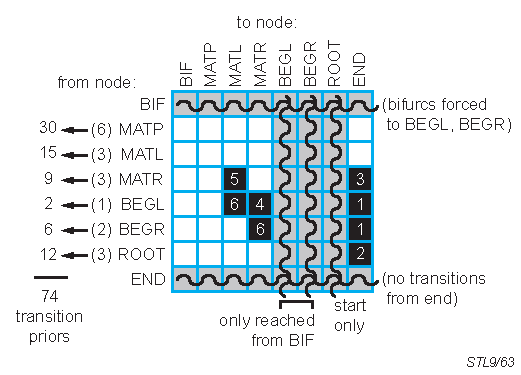
\includegraphics{Figures/stl9-63}
\end{center}
\caption{\small\textbf{Where does the magic number of 74 transition
distribution types come from?} The transition distributions are
indexed in a 2D array, from a unique statetype (20 possible) to a
downstream node (8 possible), so the total conceivable number of
different distributions is $20 \times 8 = 160$. The grid represents
these possibilities by showing the $8 \times 8$ array of all node
types to all node types; each starting node contains 1 or more unique
states (number in parentheses to the left).
Two rows are impossible (gray): bifurcations automatically transit to
determined BEGL, BEGR states with probability 1, and end nodes have no
transitions.  Three columns are impossible (gray): BEGL and BEGR can
only be reached by probability 1 transitions from a bifurcation, and
the ROOT node is special and can only start a model. 
Eight individual cells of the grid are unused (black) because of the
way \prog{cmbuild} (almost) unambiguously constructs a guide tree from
a consensus structure.  These cases are numbered as follows. (1) BEGL
and BEGR never transit to END; this would imply an empty
substructure. A bifurcation is only used if both sides of the split
contain at least one consensus pair (MATP). (2) ROOT never transits to
END; this would imply an alignment with zero consensus
columns. Infernal models assume $\geq 1$ consensus columns. (3) MATR
never transits to END. Infernal always uses MATL for unpaired columns
whenever possible. MATR is only used for internal loops,
multifurcation loops, and 3' bulges, so MATR must always be followed
by a BIF, MATP, or another MATR. (4) BEGL never transits to MATR. The
single stranded region between two bifurcated stems is unambiguously
assigned to MATL nodes on the right side of the split, not to MATR
nodes on the left. (5) MATR never transits to MATL. The only place
where this could arise (given that we already specified that MATL is
used whenever possible) is in an interior loop; there, by unambiguous
convention, MATL nodes precede MATR nodes. (6) BEGL nodes never
transit to MATL, and BEGR nodes never transit to MATR. By convention,
at any bifurcated subsequence $i,j$, $i$ and $j$ are paired but not to
each other. That is, the smallest possible subsequence is bifurcated,
so that any single stranded stretches to the left and right are
assigned to MATL and MATR nodes above the bifurcation, instead of MATL
nodes below the BEGL and MATR nodes below the BEGR.
Thus, the total number 74 comes from multiplying, for each row, the
number of unique states in each starting node by the number of
possible downstream nodes (white), and summing these up, as shown to
the left of the grid.}
\label{fig:magic74}
\end{figure}

\newpage
\section{Acknowledgements and history}

HMMER 1 was developed on slow weekends in the lab at the MRC
Laboratory of Molecular Biology, Cambridge UK, while I was a postdoc
with Richard Durbin and John Sulston. I thank the Human Frontier
Science Program and the National Institutes of Health for their
remarkably enlightened support at a time when I was really supposed to
be working on the genetics of neural development in \emph{C. elegans}.

HMMER 1.8, the first public release of HMMER, came in April 1995,
shortly after I moved to Washington University in St. Louis. A few
bugfix releases followed. A number of more serious modifications and
improvements went into HMMER 1.9 code, but 1.9 was never
released. Some versions of HMMER 1.9 inadvertently escaped St. Louis
and make it to some genome centers, but 1.9 was never documented or
supported. HMMER 1.9 collapsed under its own weight in 1996.

HMMER 2 was a nearly complete rewrite, based on the new Plan 7 model
architecture. Implementation was begun in November 1996. I thank the
Washington University Dept. of Genetics, the NIH National Human Genome
Research Institute, and Monsanto for their support during this time.
Also, I thank the Biochemistry Academic Contacts Committee at Eli
Lilly \& Co. for a gift that paid for the trusty Linux laptop on which
much of HMMER 2 was written. The laptop was indispensable. Far too
much of HMMER was written in coffee shops, airport lounges,
transoceanic flights, and Graeme Mitchison's kitchen. The source code
still contains a disjointed record of where and when various bits were
written.

HMMER then settled into a comfortable middle age, like its primary
author -- still actively maintained, though dramatic changes seemed
increasingly unlikely. HMMER 2.1.1 was the stable release for three
years, from 1998-2001.  HMMER 2.2g was intended to be a beta release,
but became the \emph{de facto} stable release for two more years,
2001-2003. The final release of the HMMER2 series, 2.3, was assembled
in spring 2003.  The last bugfix release, 2.3.2, came out in October
2003.

If the world worked as I hoped and expected, the combination of the
1998 Durbin/Eddy/Krogh/Mitchison book \emph{Biological Sequence
  Analysis} and the existence of HMMER2 as a widely-used proof of
principle \emph{should} have motivated the widespread adoption of
probabilistic modeling methods for sequence analysis, particularly
database search. We would declare Victory and move on. Richard Durbin
moved on to human genomics; Anders Krogh moved on to pioneer a number
of other probabilistic approaches for other biological sequence
analysis problems; Graeme Mitchison moved on to quantum computing; I
moved on to noncoding RNAs.  

Yet BLAST continued to be the most widely used search program.  HMMs
seemed to be widely considered to be a mysterious and orthogonal black
box, rather than a natural theoretical basis for important programs
like BLAST. The NCBI, in particular, seemed to be slow to adopt or
even understand HMM methods. This nagged at me; the revolution was
unfinished!

When we moved the lab to Janelia Farm in 2006, I had to make a
decision about what we should spend our time on. It had to be
something ``Janelian'': something that I would work on with my own
hands; something that would be difficult to accomplish under the usual
reward structures of academic science; and something that would make
the largest possible impact on science. I decided that we should aim
to replace BLAST with an entirely new generation of software. The
result is the HMMER3 project.

\subsection{Thanks}

HMMER is increasingly not just my own work, but the work of great
people in my lab, including Steve Johnson, Alex Coventry, Dawn Brooks,
Sergi Castellano, Michael Farrar, Travis Wheeler, and Elena Rivas.
The current HMMER development team at Janelia Farm includes Sergi,
Michael, and Travis as well as myself.

I would call the Janelia computing environment world-class except that
it's even better than that. That's entirely due to Goran Ceric. HMMER3
testing now spins up thousands of processors at a time, an unearthly
amount of computing power.

Over the years, the MRC-LMB computational molecular biology discussion
group contributed many ideas to HMMER. In particular, I thank Richard
Durbin, Graeme Mitchison, Erik Sonnhammer, Alex Bateman, Ewan Birney,
Gos Micklem, Tim Hubbard, Roger Sewall, David MacKay, and Cyrus
Chothia.

The UC Santa Cruz HMM group, led by David Haussler and including
Richard Hughey, Kevin Karplus, Anders Krogh (now back in Copenhagen)
and Kimmen Sj\"{o}lander, has been a source of knowledge, friendly
competition, and occasional collaboration. All scientific competitors
should be so gracious. The Santa Cruz folks have never complained (at
least in my earshot) that HMMER started as simply a re-implementation
of their original ideas, just to teach myself what HMMs were.

In many places, I've reimplemented algorithms described in the
literature. These are too numerous to credit and thank here. The
original references are given in the comments of the code. However,
I've borrowed more than once from the following folks that I'd like to
be sure to thank: Steve Altschul, Pierre Baldi, Phillip Bucher, Warren
Gish, Steve and Jorja Henikoff, Anders Krogh, and Bill Pearson.

HMMER is primarily developed on GNU/Linux and Apple Macintosh
machines, but is tested on a variety of hardware. Over the years,
Compaq, IBM, Intel, Sun Microsystems, Silicon Graphics,
Hewlett-Packard, Paracel, and nVidia have provided generous hardware
support that makes this possible. I owe a large debt to the free
software community for the development tools I use: an incomplete list
includes GNU gcc, gdb, emacs, and autoconf; the amazing valgrind; the
indispensable Subversion; the ineffable perl; LaTeX and TeX;
PolyglotMan; and the UNIX and Linux operating systems.

Finally, I will cryptically thank Dave ``Mr. Frog'' Pare and Tom
``Chainsaw'' Ruschak for a totally unrelated free software product
that was historically instrumental in HMMER's development -- for
reasons that are best not discussed while sober.

\label{manualend}


\newpage
\bibliography{master,lab,books,local}
\end{document}

\clearpage
\section{\TT{params}}

\subsection{Model parameter specification}

The \TT{params} routine reads the file specified as the first argument on the \NAME\ command
line (usually "something.run"), or by default, "test.run" if no name is given.  The main
purpose of the \TT{params} routine is to read a file of parameters (specified by the
\Tt{PARAMS} command described below) and set-up the generic behaviours for each level in
the model hierarchy.

Each property is specified
on one line as a series of integers corresponding to successively deeper levels.  There
can be up to 10 levels and unused fields are left as trailing zeros which can be followed
by an optional comment.   Presently, there are also ten different properties specified
by the parameter file which will be described below.  (With their parameter name italicized
in the sub-section title).

Firstly however, the routine expects a
declaration of the molecule type, which can be any of: \Tt{PROT}, \Tt{RNA}, \Tt{DNA},
\Tt{CHEM} or \Tt{CELL}.  Any other text will probably behave in a protein-like way.
This can be followed by a secondary command that is used by the \TT{viewer} to specify
a colour scheme for rendering which will be described under the section on that routine.

Except for models specified as \Tt{CHEM}, 
it is assumed that the lowest (most detailed) level of the molecular representation will
be a backbone 'virtual' chain, without any atomic detail.  

\subsubsection{\Tt{Line 1}: {\em type} of object}

As described above, there can be three types of object, a: sphere, tube and ellipsoid that
are specified by the numbers 1,2,3, respectively.   There can also be a virtual object that
can have all the properties of a sphere but just is not rendered except as a tiny sphere.
Ellipsoids (with axis lengths, $A,B,C$) can only be oblate ($A<B=C$) or prolate ($A>B=C$).
These shapes are generally, referred to as spheroids but the term ellipsoid will be retained
below to maintain a distinction from the sphere-object (which persists even when $A=B=C$).

If a negative number is specified, then the object is rendered as a wire mesh but otherwise
behaves identically.

\subsubsection{\Tt{Line 2}: {\em size} of object}

The second line specifies the size of the object.  For spheres and tubes, this is the diameter
while for ellipsoids it is the diameter across the axis of symmetry ($B$ or $C$, in the above 
specification).   The values specified here are used at a tenth their size inside \NAME.

With a specified known type of molecule (protein of nucleic acid), standard values will be
adopted and maintained for bond lengths and internal secondary structure links (more below).
This means that higher levels (eg: protein domains) are free to move within their specified
constraints.  While this is usually the normal desired behaviour, it is sometimes required
that the local starting geometry of the configuration should be preserved.  This is implemented
by the \TT{fixer} and a negative prefix on the \Tt{size} value will signal that it should be
applied during the simulation to that level of structure. 

\subsubsection{\Tt{Line 3}: {\em bump} size of object}

Although it might be assumed that objects will bump when their surfaces make contact, however,
there are situations where it is useful to have a different bump size, which can be specified
on this line.

\subsubsection{\Tt{Line 4}: number of {\em links}}

Any object can form links to any other object (on the same level).  To avoid allocating unused
space to objects that never link, the maximum number of links can be specified on this line. 

\subsubsection{\Tt{Line 5}: number of {\em bonds}}

The number of bonds an object can make is specified in an identical manner but has some
implications for polymers (protein, nucleic acid) that are expected to form chains.

Specifying a non-zero number of bonds for a polymer automatically results in the creation
of bonds between adjacent monomers within their group. 
So in the \Tt{GROUP} structure declared in the previous section, if bonds
were specified at the atomic level, then there would be two chains of 3 and 4 monomers.
If bonds were allocated to the next level up (normally the secondary structure level), then
a chain of two secondary structures would be created.  However, for consistency, the
program will also create the bond joining their two atomic level chains (giving a single
chain of 7 monomers at the 'atomic' level).  If the atomic level has no bonds, then each
secondary structure in the chain will contain a group of free-floating atoms.

If the number of bonds specified is negative, this is taken as a flag to create a circular
chain.  So in the current example, a negative number on the atomic level will create two
circular chains of 3 and 4 monomers.   If the secondary structure level is also negative,
and the atomic level positive, there will be a 'ring' of 2 secondary structures containing 
a ring of 7 monomers and if both values are negative, the 'ring' of 2 will contain a
triangle and square 'rings' with no bond between them.

In some higher level polymer domain configurations and chemical structures, each object
may form multiple bonds and the value of the bond number is equivalent to the maximum
valance of the object.  

\subsubsection{\Tt{Line 6}: {\em move} step size}

The step size applied by the \TT{shaker} is specified on this line.   As with all motion,
it is applied from the top level downwards with every movement at the higher level also
propagated to all offspring below.

If the specified value of $size$ ($S$) is positive, the motion is a translation in a random direction
with a magnitude of $S$/100, followed by a rotation in a random direction with a angular
displacement of $S$/100 radians.

If the value is negative, then just the translation is applied.

\subsubsection{\Tt{Line 7}: {\em keep} within parent boundaries}

If a child strays outside its parent's boundary (as defined by its $size$), then a shift
(or kick) is applied to redirect it inwards with a magnitude specified on this line.
Note that the value appears in the position of the level of the parent but is applied
to the level below).

If the parent is a sphere, then 'inwards' is towards its centre  and for an ellipsoid,
'inwards' is towards the nearest focus (simpler than calculating surface normals).  For a tube,
the default action is to shift the child towards the surface whether inside or outside
the tube, in a direction perpendicular to the tube axis.

If the value of the parameter is negative, then these default actions are reversed and
children within spheres and ellipsoids will be directed towards the parental surface
while children will be free to wander inside the tube.

Some of these behaviours can be modified for individual objects by values specified in
the model description read in the \TT{models} routine described below.

\subsubsection{\Tt{Line 8}: {\em bond} length}

The bond lengths specified on this line are the default ideal values which every bond
associated with that level will be refined towards.  As not all objects are spheres, the
bond length is not a simple centre---centre distance.   For spheres, it is the distance
between the surfaces (so the centre---centre distance = $bond+size$).  For tubes, it is
the desired separation between the ends of two tubes (axis end---end distance) and for
ellipsoids it is the equivalent pole---pole distance between the ends of their axes of
symmetry.  (The ends of the $A$ axis, in the example above.).

A negative value of the bond length evokes a behaviour that prevents the default joining
of chains of children when their parents are in a chain.  This is 
useful when constructing a fiber formed from unbonded subunits (such as actin).

\subsubsection{\Tt{Line 9}: {\em hard} bump repulsion}

The way in which objects bump is simple only at the atomic level where a kick is applied
to both atoms in a direction away from their common centre with a magnitude of $M$/100,
where $M$ is the specified value.  This repulsion is applied when the distance between
the atom centres is less than the value of $bump$ and is independent of the degree of
penetration or any other constraint.

\subsubsection{\Tt{Line 10}: {\em soft} bump repulsion}

Objects at a higher level do not behave in this way but can 'happily' inter-penetrate,
providing none of their children are clashing.   The degree to which they are separated
is a function of the number of inter-family bumps on a non-linear scale between the value
of the $hard$ repulsion specified on the previous line and the $soft$ value specified
on this line.  Specifically, the kick size, $k$, is: $k = g*S + (1-g)*H$, where $S$ 
and $H$ are the $hard$ and $soft$ values and $g = \exp (-m^2)$, for $m$ child collisions.

As the value of $g$ ranges from 1 (no bumping children) to 0 (many bumping children) the
degree of parental repulsion will scale from $soft$ to $hard$.   This means that if $soft$
has a non-zero value, then there will be a 'soft' repulsion before any of the children in the
two families clash.  This creates a 'jelly' like behaviour to the collision of high-level
objects.

If the value of $soft$ is negative, then behaviour of the objects reverts to hard repulsion.

\subsection{An example input file}

\begin{singlespace}
------------------------------------------------------------------------------------------------------
\begin{footnotesize}
\begin{verbatim}
PROT sec
    0,    0,    3,    2,    1,    0,    0,    0,    0,    0    	// type
 9999, -120,  -50,   -8,    2,    0,    0,    0,    0,    0    	// size
    0,  120,   50,    8,    8,    0,    0,    0,    0,    0    	// bump
    0,    0,    0,    6,    4,    0,    0,    0,    0,    0    	// nlinks
    0,    0,    0,    1,    1,    0,    0,    0,    0,    0    	// nbonds
    0,    0,    1,    1,    1,    0,    0,    0,    0,    0    	// move
    0,    2,    5,   10,    0,    0,    0,    0,    0,    0    	// keep
    0,    0,    0,    0,    4,    0,    0,    0,    0,    0    	// bond
    0,   10,   10,   10,   10,    0,    0,    0,    0,    0    	// hard bump
    0,    1,    2,    5,    0,    0,    0,    0,    0,    0    	// soft bump
\end{verbatim}
\end{footnotesize}
------------------------------------------------------------------------------------------------------
\end{singlespace}

In this example, a protein model is set-up with 4 levels (not including the world).
From bottom up, the levels corresponds to: \CA-chain, secondary structure elements,
domains and individual chains (subunits). 

The first column describes the world simply as big (9999).  Other values can be assigned to
the world and, except that it will not move or be rendered, it is a normal object.
A useful behaviour is to give it a smaller size and assign a value to $keep$ to stop
objects wandering too far away. 

The atomic level (fifth column) specifies each atom is a small sphere ($size = 2$) and is in
a linear chain ($nbonds > 0$).  So with a relatively long bond between atoms ($bond = 4$),
the chain will will appear as a "ball-and-stick" model (with an atom---atom distance of 6). 
It has a bump size that is larger than this ($bump = 11$) but as bonded atoms do not bump (more
detail in the \Tt{bumper} section), this will first apply to neighbours-but-one along the chain,
keeping the virtual bond angle along the chain almost obtuse. (Since $6*6+6*6 \approx 8*8$).
The value of 8 was chosen as it is the closest approach made between monomers in an \AH\ and
as linked atoms do bump, this will avoid disruption. (In \AA ngstroms, this is 8*3.8/6 = 5.1
which is close to the i---i+2 distance in the \AH)). 
Each atom has the capacity to make 4 links, two of which will be automatically used in local
secondary structure formation).  The atoms will have a slight motion and a reasonably strong
($hard$) bump repulsion.

The secondary structure level is a chain ($nbonds = 1$) of tubes ($type = 2$) with equal
$size$ and $bump$ values that just enclose their atomic configurations. Note that the $size$
values at this level and above are negative, indicating that there is no generic bond length 
and local geometry will be preserved by the \Tt{fixer}.   If the $size$ value were positive,
the \TT{linker} would enforce the generic bond length, which is set at zero, and would link
the tubes without any spacer.  So not a disaster, but causing a marked shift away from
the original structure once the simulation is started.  Quite a few links are allocated (6)
and as none are automatically assigned at this level (?), there is scope to tie-down the 
structure further.  A value of $keep$ is specified to hold the atoms to the tube surface
(except in loop regions where this is not enforced).
Both the $hard$ and $soft$ bump settings are now used so the secondary
structures have a bit of a jelly-like constitution.

At the next higher (domain) level, the objects are ellipsoids (of softer jelly) and are still
in a chain.  Parents are also a bit more relaxed about keeping their children close.  These
trends continue to the next (subunit) level which is no longer chained and is rendered as a
virtual sphere ($type = 0$).
 

\subsection{Global value specification}

Although the main purpose of \TT{params} is to parameterise the model behaviour, it also
sets-up some general behaviours most of which are used in 'debugging' the model specification
script described in the next section.   These commands should generally be specified in the
order in which they are described below.

\subsubsection{\Tt{NORUN}}

Compile and run the model but do not execute the \TT{driver} routine.

\subsubsection{\Tt{NOMOVE}}

Compile and run the model but do not execute the \TT{shaker}, \TT{keeper} or \TT{bumper} routines.
This command is very useful for checking (and as the \TT{viewer} is active, seeing) if the model 
is OK before it has the chance to do anything (like explode).

\subsubsection{\Tt{NOVIEW}}

The \TT{viewer} is not executed.   Essential for use in batch mode, say on a computer cluster.

\subsubsection{\Tt{HIDDEN}}

Freezes execution of objects that are out of view, either outside the field-of-view or
beyond the back-plan or behind the point-of-view.   Distant objects also become solid and
their contents is also frozen.

\subsubsection{\Tt{SCALE <in> <out>}}

Sets two scale factors, the first is applied to all coordinates read in by \TT{models} and the
second to coordinates written out (usually from \TT{looker}).  Default values are used for
protein and nucleic acid for input but when writing very large structures in PDB format, a
small scale factor is often needed to get the values to fit the format.

The line: {\tt SCALE 0.158 0.633  \# scalein = .6/3.8, scaleout = 3.8/6}, scales a PDB input
to have a CA---CA bond length of 0.6 and an output scale of 0.38 (tenth size).

\subsubsection{\Tt{SHRINK <value>}}

This scale factor is applied on every simulation cycle to the highest level (1, not counting
the world). A factor of $1-<value>$ is applied to the positions of all level-1 objects causing
them to fall towards the centre of the world.   Its main use has been in testing collisions
as it saves time waiting for wandering objects to collide.

\subsubsection{\Tt{PARAM <filename>}}

This is the key command that specifies the name of the file containing all the model parameters
described in the first section.  It is usually called "something.model".

Up to five models can be introduced by separate \Tt{PARAM} lines and are assigned numbers
starting with zero upwards, in order of their occurrence.

\subsubsection{\Tt{END}}

Marks the end of the parameter input stage and the start of the model description.




%#include "util.hpp"
%#include "geom.hpp"
%#include "cell.hpp"
%#include "data.hpp"
%
%void paramin ( char*, int );
%
%int params ( FILE *run ) {
%// read the global behaviour values and model data
%// NB commands must come in the order specified below as there is no loop 
%int	n, io, nmodels;
%float	s, sget, sput;
%char	line[222];
%	Data::shrink = 0.0;	// used as 1-shrink (-ve = mass factor)
%	Data::scalein = 0.1;	// default unless specified by SCALE <in> <out>
%	Data::scaleout = 1.0;	// unless specified by SCALE
%	LOOP {
%		io = read_line(run,line);
%		if (io < 0) { Pt(Unexpected end of file\n) exit(1); }
%		if (io==0) continue;
%		if (line[0]=='#') continue; // NB comments (#) only at start
%		break;
%	}
%	if (line[0]=='N' && line[2]=='R') {
%		Data::norun = 1;		// NORUN flag (skip driver)
%		read_line(run,line);
%	}
%	if (line[0]=='N' && line[2]=='M') {
%		Data::norun = 2;		// NOMOVE flag (no linker,shaker,bumper) 
%		read_line(run,line);
%	}
%	if (line[0]=='N' && line[2]=='V') {
%		Data::noview = 1;		// NOVIEW flag (skip viewer)
%		read_line(run,line);
%	}
%	if (line[0]=='H' && line[2]=='D') {
%		Data::hidden = 1;		// HIDDEN flag (skip viewer)
%		if (io > 7) {
%			sscanf(line+6,"%d", &n);
%			Data::hidden = n;
%		}
%		read_line(run,line);
%	}
%	if (line[0]=='S' && line[1]=='C') { // output SCALE factor (saved in world->far)
%		Ps(line) NL
%		sscanf(line+6,"%f %f", &sget, &sput);
%		Data::scalein = sget;
%		Data::scaleout = sput;
%		read_line(run,line);
%	}
%	if (line[0]=='S' && line[2]=='R') { // SHRINK factor (saved later in scene->far)
%		Ps(line) NL
%		sscanf(line+7,"%f", &s);
%		Data::shrink = s;
%		read_line(run,line);
%	}
%	if (line[0] != 'P') {
%		printf("Need a PARAM filename\n");
%		return 2;
%	}
%	nmodels = 0;
%	while (1) { char atomtype; // read in param file(s)
%		printf("Reading parameters from %s\n", line+6);
%		paramin(line+6,nmodels);
%		nmodels++;
%		read_line(run,line);
%		if (line[0] == 'P') continue;
%		if (line[0] == 'M' || line[0] == 'E') { // MODEL or END to finish
%			printf("End of parameters\n\n");
%			Pt(Read) Pi(nmodels) NL
%			DO(i,nmodels) // set the atomic bond lengths
%			{ float len = Data::model[i].sizes[Data::depth]
%				    + Data::model[i].bonds[Data::depth];
%				printf("Model %d is", i);
%				if (Data::model[i].moltype==0) { // protein
%					Data::bondCA = len;
%					Pt(protein with) Pr(Data::bondCA) NL
%				}
%				if (Data::model[i].moltype==1) { // nucleic
%					Data::bondPP = len;
%					Pt(nucleic with) Pr(Data::bondPP) NL
%				}
%				if (Data::model[i].moltype==2) { // chemistry
%					Pt(chemical) NL
%				}
%				if (Data::model[i].moltype==3) { // cells
%					Pt(cells) NL
%				}
%			}
%			break;
%		}
%		Pt(Bad) Ps(line) NL exit(1);
%	}
%	Data::nmodels = nmodels;
%	if (line[0] == 'M') { int model;
%		sscanf(line+6,"%d", &model);
%		printf("Using model %d\n", model);
%	}
%}
%
%void paramin ( char *param, int n ) {
%int	i, j, io;
%FILE	*dat;
%char	*at;
%char	line[222];
%char	name;
%Data	*model = Data::model+n;
%	dat = fopen(param,"r");
%	if (!dat) { printf("%s parameter file not found\n", param); exit(1); }
%	io = read_line(dat,line);
%	model->moltype = model->subtype = 0; // default (any protein-like chain)
%        if (line[0]=='P') model->subtype = 1; // PROTein (CA-CA = 3.8)
%        if (line[0]=='R') { model->moltype = 1; model->subtype = 0; } // RNA
%        if (line[0]=='D') { model->moltype = 1; model->subtype = 1; } // DNA
%        if (line[1]=='H') model->moltype = 2; // CHEM (needs fixing)
%        if (line[1]=='E') model->moltype = 3; // CELLs
%	model->colours = 0;		// default = colour by level
%	if (strlen(line) > 4) {
%        	if (toupper(line[5])=='S') model->colours = 1; // PROT with SSE coloured red/green
%        	if (toupper(line[5])=='B') model->colours = 2; // flash Bumps in a different colour
%	}
%	name = line[io-1];
%	i = 0;
%	while (1) {
%		Pi(i)
%		if (read_line(dat,line) < 0) break;
%		if (line[0] == '/') continue;
%		*(strstr(line,"/")) = '\0';
%		at = line;
%		for (j=0; j<N; j++) { int in;
%			sscanf(at,"%d", &in);
%			if (in != 0) Data::depth = max(Data::depth,j);
%			printf("%5d ", in);
%			at = strstr(at,","); at++;
%			switch (i) {
%				case 0 :
%					model->shape[j] = in;
%					//	-ve = render as wireframe
%					break;
%				case 1 :
%					model->sizes[j] = 0.1*(float)abs(in);
%					//	-ve = use values in prox and dist 
%					if (in<0) model->local[j] = 1; else  model->local[j] = 0;
%					break;
%				case 2 :
%					model->bumps[j] = 0.1*(float)in;
%					//	-ve
%					break;
%				case 3 :
%					model->links[j] = in;
%					//	-ve
%					break;
%				case 4 :
%					model->chain[j] = in;
%					//	-ve = circular
%					break;
%				case 5 :
%					model->kicks[j] = 0.01*(float)in;
%					//	-ve
%					break;
%				case 6 :
%					model->keeps[j] = 0.01*(float)in;
%					//	-ve = shell for types 1,3 or tube = open
%					break;
%				case 7 :
%					model->bonds[j] = 0.1*(float)in;
%					//	-ve = no bond between cousins
%					if (in<0) model->split[j] = 1; else  model->split[j] = 0;
%					break;
%				case 8 :
%					model->repel[j] = 0.01*(float)in; // hard bump
%					//	-ve don't repel children within parent
%					break;
%				case 9 :
%					model->rejel[j] = 0.001*(float)in; // soft bump
%					//	-ve don't repel children within parent
%					break;
%			}
%		} NL
%		i++;
%		if (i==N) break;
%	}
%	fclose(dat);
%}

\clearpage
\section{\TT{models}}

\subsection{Overview of the object hierarchy}

The \TT{models} routine continues reading the main input file ("test.run")
after \TT{params} has completed.  It reads-in a hierarchy of groups of objects
(as outlined in the \Tt{main} section).   Besides the basic hierarchy sketched
previously, each group declaration can be preceded by a series of commands
(referred to below as a "Move set") that specify geometric operations that
will be applied to the group and all its sub-groups.  Correspondingly, at the
end of each group, another set of instructions (called the "Bond set") can
be included to specify bonds and links or modify those that have been created
automatically.    Although the end of each group is usually identified
automatically (after all its children have been read or by the appearance of
a command that implies the end), it is convenient for the moment to use the
\Tt{TER} command which explicitly marks the end of a group. 

Using \Tt{TRANS} to represent a Move-set and \Tt{REBOND} to represent a
Bond-set, then the model outlined in the opening section can be elaborated
as it might appear in the file "test.run".  (Indentation is not required but
can help clarity).
\begin{singlespace}
---------------------------------------------------------------------------------------------------
\begin{verbatim}
        PARAM some.model
    END
        TRANS set-1
        GROUP 0 1
            GROUP 0 2
                TRANS set-2
                GROUP 0 3
                    ATOM...
                    ATOM...
                    ATOM...
                TER
                GROUP 0 4
                    ATOM...
                    ATOM...
                    ATOM...
                    ATOM...
                REBOND set-A
                TER
           TER
       REBOND set-B
       TER
   END
\end{verbatim}
\ \ \ \ ---------------------------------------------------------------------------------------------------
\end{singlespace}
The transforms specified in the first Move-set (\Tt{TRANS set-1}) will apply rotations
and translations to everything that is created whereas the second set will apply
just to the first group of 3 'atoms'.   The first Bond-set (\Tt{REBOND set-A})
could specify new bonds within the second group of 4 atoms while set-B could 
make links between and within the two groups of atoms.

Representing
a Group (\Tt{GROUP}) declaration as  \Tt{G}, 
a Move-set (\Tt{TRANS}) declaration as  \Tt{M}, 
an atomic level (\Tt{ATOM}) declaration as  \Tt{A},
a Bond-set (\Tt{REBOND}) declaration as \Tt{B} and
a group termination (\Tt{TER}) as \Tt{T};
the model in the example above could be written:
\Tt{MGGMGAAATGAAAABTTBT}.   Using this representation, each group-structure has the 
form \Tt{MGABT}, or writing the optional commands in lower-case:  \Tt{mGAbt}.
If \Tt{*} now designates any number of atoms or any number of valid group-structures,
then the input stream expected by \TT{models} is: \Tt{mG*bt}. 
Expanding each '\Tt{*}' recursively within parentheses and bracketing groups on the same 
level, the above example can be seen to be a valid stream which will be parsed as:
\Tt{MG( G( [MG( AAA )T][G( AAAA )BT] )T )BT}.

In a structure that includes many repeated substructures, it would be tedious to 
specify the group structure for each occurrence.  To avoid this, a group structure can
be contained within a file and just the filename specified (using the \Tt{INPUT} command,
of which more below) instead of a full group specification.  As different instances of
each substructure may require a different Move-set, these can precede the \Tt{INPUT}
command but the end of an input file is treated as an End-of-Group signal, so group
definitions cannot span files.    \Tt{INPUT} files can, of course, contain \Tt{INPUT}
commands.

\subsection{Move-set commands}

These are described in the order in which they are applied to the completed group.
Characters within brackets indicate options and if separated by a bar '|', are optional
strings.  Strings within angle brackets represent numbers.

\subsubsection{\Tt{TRANS  <x> <y> <z>}}

A translation of the group by a displacement vector \{x,y,z\}. 

\subsubsection{\Tt{SPIN[XYZ] <theta>}}

A rotation of the group by an angle of \Tt{theta} degrees about the specified axis
(X,Y,Z).  For example: \Tt{SPINY 90} rotates the group by 90\dgr\ around the Y-axis. 

\subsubsection{\Tt{SPINS <tx> <ty> <tz>}}

Is a more general \Tt{SPIN} command, rotating about the X, then Y, then Z axes by the three
specified angles: \Tt{tx}, \Tt{ty},\Tt{tz}.

\subsubsection{\Tt{TWIST <x><y><z> <p><q><r> <twist>}}

Rotate about the line defined from \{x,y,z\} to \{p,q,r\} by and angle \Tt{twist}.

\subsubsection{\Tt{HELIX <x><y><z> <turns>}}

Move the group by \Tt{x,y}, rotate by \Tt{<turns>} degrees about the Z axis then move \Tt{z}
along Z.    (N.B., the commands \Tt{TWIST} and \Tt{TRANS} can be combined to generate a helix
along any axis.)

\subsection{\Tt{GROUP <sort> <kids> [<x><y><z> <p><q><r>]}}

The full syntax of the \Tt{GROUP} command allows not only the the specification of the number
of expected children (\Tt{kids}) but also the \Tt{sort} of group that is wanted.   This is an
integer number that acts on a non-spherical object type (tube or ellipsoid) to modify its length.  
This is not something that can  be specified in the parameter file as each object will typically
have a different length depending on the number of atoms it contains.

The axis of these objects can also be specified as two additional end-point coordinates
(\{x,y,z\} and \{p,q,r\}).

\subsubsection{Tubes}

If the molecule type is protein and the group is at the secondary structure level (one up 
from atomic) then the \Tt{sort} value is used to specify secondary structure sort as:
0 = loop, 1 = an \AH\ and 2 = a \Bs.   Each have a particular tube length/thickness ratio
determined by the helical rise/residue along the secondary structure and the expected bulk
for a given loop length.  For each sort (0,1,2) the values used are: 0.5, 1.5, 3.0.
If the end-points are unspecified, then the axis is estimated from the terminal residues.
Even when the axis is specified, it provides only the direction and is set to pass through
the centre of the object.

If the molecule type is nucleic acid, the length is set in a similar manner using the
known rise/basepair.

Tubes that are not associated with a known secondary structure can have their length specified
by the value of \Tt{sort}, either as a multiple of their thickness (up to 10 times) or if
the value is negative, by the distance between the end-points (which must then be provided). 

\subsubsection{Ellipsoids}

As there are no secondary structures automatically associated with the ellipsoid shape, the
length of the ellipsoid axis is set only by the value of \Tt{sort} but whereas the value for a
tube was a simple ratio (1..10), the value for an ellipsoid runs from 1..21 with values over
10 creating oblate shapes and under 10, prolate shape (10=spherical).  The scaling is not 
linear but follows the progression: $n/10$ up to 10 and $10/n$ over 10 where $n = abs(10-sort)$.

Any negative value of \Tt{sort} again causes the length of the specified axis to be used. 

\subsubsection{Nucleic acids}

For both RNA and DNA, the \Tt{GROUP} command can adopt a two aliases, \Tt{DOUBL} and \Tt{SINGL},
to deal with differences between double and single stranded segments.  The latter is in fact
identical to  \Tt{GROUP} and was included just for neatness but the \Tt{DOUBL} command uses
the value of  \Tt{sort} to label a strand (Watson) that requires a complementary strand (Crick)
to occur later with the negated value of \Tt{sort}.

The default construction for nucleic acids treats a base-pair as a secondary structure so when
a \Tt{DOUBL} command is encountered, rather than allocating the specified number of \Tt{kids}
as individual atoms, the equivalent number of two-atom groups (basepairs) are created and the
following \Tt{ATOM} records are used to fill the first child in each basepair.   When the 
complementary strand is encountered, the the second child is then filled (running backwards).
Clearly, complementary strands must be equal in length and the first atom in Watson will be
basepaired with the last atom in Crick. 


\subsection{Bond-set commands}

\subsubsection{{\tt REBOND} and {\tt REJOIN} commands}

The commands that create and modify a chain take the form: {\tt RE[BOND|JOIN|TERM] mode <from> <to>}.
For example {\tt REBOND pdbid 22 66} sets a bond between the atoms with a residue numbers 22 and 66.
But what if the residue numbers in the PDB file (which became \Tt{ATOM} records are inconsistent or
missing or, as is likely, residues 22 and 66 are already bonded?

So as not to rely on PDB specified residue numbers \NAME\ maintains three internal atom counts as
well as a separate count of all objects (called their Unique IDentifier, or UID).  The {\tt allatom}
count starts with the first and ends with the last.  The {\tt teratom} count is set to zero with the
start of each group and between these is the {\tt endatom} count that is re-zeroed automatically by
any Bond-set command or explicitly by an {\tt INPUT} command with a zero appended ({\tt INPUT0}).

These numbering schemes are selected by the {\tt mode} string which can be set as: {\tt group}, {\tt local},
{\tt atomid}, {\tt unique} and {\tt pdbid}, referring respectively to the  {\tt teratom},  {\tt endatom}
and  {\tt allatom} counts, the UID and the PDB number.   The first two can obviously only be used
withing a level of nesting (scope) where their values have not been re-zeroed but the {\tt atomid} and
{\tt unique} counts are universal.   The uniqueness of the PDB numbering depends both on the
original source and how often it is reread using the {\tt INPUT} command, so must be used cautiously.

Only the {\tt unique} values can be used to rewire objects higher than the atomic level but this
must be done carefully as internal consistency checks refer only to the atomic level chain (see below).

The {\tt REJOIN} command has an identical syntax and operation but creates a virtual bond that is
not refined or rendered. (In other words it makes a gap in the chain).

Both commands overwrite whatever existing bond may have been there so after a series of reconnections,
there may be no free termini.  To avoid this, the {\tt RETERM} command can be used to specify new
start and final positions of the chain using the {\tt from} and {\tt to} fields as start and end.
Again, care must be taken as the inclusion of a {\tt RETERM}
command triggers the execution of the internal consistency check described below.  Otherwise it
is assumed that the rewiring operations are harmless. 

\subsubsection{Rewiring consistency}

Even when applied properly, the above commands have the potential to alter the chain topology
of the polymer leaving the higher levels out-of-step with the chain at the atomic level.
To restore consistency, once all the groups have been completed, a subroutine traces the new
chain path at the atomic level and renumbers the higher levels in a sequential order.
This process is only executed if there is one or more {\tt RETERM} commands with each new
terminus taken as a start point.  So if the chain topology has been altered but the termini
remain the same, a {\tt RETERM} command re-specifying the original termini must be included.

At the domain level (atomic-2) and above, the atomic level chain can make multiple
entries and exits from the same object leading to branched topologies.
To accommodate branched topologies, the original bond allocation must be equal to the maximum
valance encountered on each level.   The recalculated numbering of the higher level objects then 
follows the order in which they are encountered by a path (a double linked-list) that outlines 
the topology tree.  (See the actin example below for clarification). 

\subsubsection{{\tt BONDS} and {\tt LINKS} commands}

The {\tt BOND} and {\tt LINK} commands operate irrespective of whether there is any polymer chain
and each follow the same syntax to read a list of simple bond/link assignments, as:
{\tt [LINKS|BONDS] mode filename}, where {\tt mode} is the numbering scheme to be used (as described
above) and the {\tt filename} contains a list of lines of four numbers specifying:
{\tt <donate> <accept> <type> <link>}.   The value of {\tt type} sets the bond thickness on
rendering or how far a link can extend without breaking and {\tt link} value is used to determine
which ends to join between elongated objects.  (More below).

Unlike the {\tt RE[BOND|JOIN]} commands, {\tt BONDS} and {\tt LINKS} will not
overwrite an existing bond/link but will fill the first free slot in the bond/link list of the
donor object.   In the context of a chain, they behave as cross-links and if the {\tt BONDS} are
specified after any {\tt RETERM} command will not alter the chain topology.

\subsubsection{{\tt SHEET} and {\tt BETA} commands}

This pair of commands are a specialised version of the {\tt LINKS} command, described above,
and are used to create cross-links between strands in a \BS.   As would be expected they can
be used only when the molecule type is a protein.

The command {\tt SHEET [mode]}, alerts \TT{models} to expect a series of links, but rather than
open a new filename, these are just read from the current stream with each link specified by the
command {\tt BETA <donate> <accept> <strength>}.   Generally, these commands are kept within
the group that contains the sheet although links between groups can be defined (I think).

The string {\tt mode} specifies the numbering scheme as described above and if omitted the
default numbering is the local group atom number.
%
%#include "util.hpp"
%#include "geom.hpp"
%#include "cell.hpp"
%#include "data.hpp"
%
%//#define MAXIN 100000 //(needed for 3chy/unit3+.run)
%#define MAXIN 100000
%#define DEEP  10
%
%typedef struct {
%	int	grows, helix, twist, shift, spins, trans;
%	Vec	grow,  move,  spin,  tran;
%	float	turns, theta;
%	Seg	axis;
%	int	set;
%} Moves;
%
%void setCell ( Cell*, int, int, int, int, int );
%void setAtom ( Cell*, char* );
%void getEnds ( Cell*, char* );
%void endCell ( Cell*, Moves* );
%int  paired ( Cell*, int, int );
%int  moveSet ( char*, Moves* );
%void newPath ( char*, char );
%int  setModel ( char* );
%FILE* getInput ( char*, Moves* );
%void pass1set ( FILE* );
%void pass2set ( Cell*, int );
%void pass3set ( Cell*, int );
%void zipDNA ( Cell* );
%void setSheet ( FILE* );
%void setAngle ( Cell*, int );
%void readlinks( char* );
%int  makeLink ( Cell*, Cell*, int, int );
%int  makeBond ( Cell*, Cell*, int, int );
%void rebond ();
%void rewire ( Cell* );
%
%Cell    **atom1cell, **atom2cell, **secs2cell;
%int      *atom2atom,  *atom2resn,  *resn2atom;
%
%Vec	cent;
%int	secs, atoms, teratoms, endatoms, allatoms;
%
%typedef struct {
%        Cell   *at, *to, *scope; // cell source, target, scope of relink
%        int     ends;     //  0 = relink, -1 = new start, 1 = new finish
%} Relinks;
%Relinks *relink;
%int     nrelinks;
%
%void models ( FILE *run )
%{
%int	i,j,k,n, wait;
%Cell	*world = Cell::world;
%	world->model = world->level = world->uid = world->id = 0;
%	secs = teratoms = endatoms = allatoms = 0;
%	model = nrelinks = 0;
%        // allocate pairs of cell to collect chain relinks in pass1set
%        relink = new Relinks[MAXIN];
%	Cell::uid2cell = new Cell*[MAXIN*8]; TEST(Cell::uid2cell) // global back-ref.lookup (total)
%	atom2cell = new Cell*[MAXIN*6];	// lookup array for all atoms (allatoms)
%	secs2cell = new Cell*[MAXIN*1];	// WAS 10000);	// lookup for all SSEs
%	atom1cell = new Cell*[MAXIN*1];	// WAS 1000);	// lookup for domain (teratoms)
%	atom2resn = new int[MAXIN*6];	// lookup from global atom id to pdb resid (allatoms)
%	atom2atom = new int[MAXIN*4];	// lookup from local to global atom id (endatoms)
%	resn2atom = new int[MAXIN*1];	// lookup from global pdb resid to atom id
%	Cell::uid2cell[0] = world;
%	Cell::total = 0;
%	pass1set(run);
%	pass2set(world,0);
%	pass3set(world,0);
%	DO(i,Cell::total) Cell::uid2cell[i]->done = 0;
%	if (nrelinks) rebond(); // remake connections at the atomic level and propagate upwards
%	DO(i,Cell::total) Cell::uid2cell[i]->done = 0;
%	// set-up the scene data
%	world->solid = -1;
%	world->live = 999;
%/*
%	for (i=0; i<SPARE; i++) { // contents allocated in copyCell()
%		n = world->kids + i;
%		world->child[n]->kids = -1; // flag that no childern exist
%		world->child[n]->nbonds = -1; // or bonds to them
%		world->child[n]->nlinks = -1; // or links to them
%	}
%	world->link = uid2cell; // world is never linked so using link to pass uid2cell address
%*/
%	Pi(Cell::total) NL
%	DO(i,world->kids) setAngle(world->child[i],0);
%	printf("Data structures all setup\n");
%}
%
%void rezero ( Moves *holds ) {
%	holds->set = 0;
%	holds->grows=holds->helix=holds->twist=holds->shift=holds->spins=holds->trans=0;
%	holds->grow.zero(); holds->move.zero();holds->spin.zero();holds->tran.zero();
%	holds->turns = holds->theta = 0.0;
%}
%
%void pass1set ( FILE *runfile ) {
%// read the command <file> to allocate memory, set values and coordinates
%/* command syntax
%	M = MOVEset = {TRANS, SHIFT, SPIN, HELIX,...} applied to the scope of the GROUP they precede
%	G = GROUP   = a group of GROUPs or ATOMs
%	A = ATOM    = atomic level coordinate (PDB format)
%	T = TER     = end the GROUP (but ends automatically when full (all kids are read)
%	B = BONDset = {BOND, LINK, REBOND, RELINK}  (see below for scope)
%  with, lower-case = optional and X* = repeat X, a block has the structure:
%	MGATB or mGAtb or mGA*tb or mG*A*t*b or (mG*A*t*b)*
%  each time a GROUP is opened, the value of <level> increases and decreases on close
%eg: 
%-------------------------------------------
%level.id (0.0 = world)
%1.0	GROUP 0 3
%2.0	GROUP 0 6
%3.0	ATOM      1  CA  GLY A   1     -23.868 -17.022  -6.339  1.33  1.00
%:	:
%3.5	ATOM      6  CA  GLY A   6     -17.825 -16.538  -2.703  1.33  1.00
%2.1	GROUP 2 5   -14.79 -14.10 -3.15   -4.36 -8.33 -0.83
%3.0	ATOM      7  CA  GLY A   7     -14.841 -14.717  -4.363  1.33  2.00
%:	:
%3.4	ATOM     11  CA  GLY A  11      -4.370  -7.485  -0.937  1.33  2.00
%2.2	GROUP 0 6
%3.0	ATOM     12  CA  GLY A  12      -1.017  -8.244   0.718  1.33  1.00
%:	:
%3.5	ATOM     17  CA  GLY A  17      -3.385  -6.721   4.645  1.33  1.00
%1.1	GROUP 0 1
%2.3	GROUP 0 6
%3.0	ATOM      1  CA  GLY A   1     -23.868 -17.022  -6.339  1.33  1.00
%:	:
%3.5	ATOM      6  CA  GLY A   6     -17.825 -16.538  -2.703  1.33  1.00
%-------------------------------------------
%DO(i,10) group[i] = group[0];
%Pi(level) Pt(at) DO(i,4) printf("%3d", at[i]); Pt(uid) DO(i,4) printf("%3d", group[i]->uid); NL
%*/
%char	full[222], *line, have, last = 'G'; // the start state
%int	level = 0, at[DEEP], setMove, deep, sheet, model = 0;
%Cell	*cell, *group[DEEP]; group[0] = Cell::world;
%FILE	*files[DEEP], *file;
%Moves	moves[DEEP], holds[1];
%int	place, baseN, baseC, basepair = 0, print = 0;
%	deep = 0;
%	files[0] = file = runfile; // current file
%	DO(i,DEEP) { at[i] = moves[i].set = 0; }
%	holds->set = 0;
%	depth = Data::depth;
%	LOOP // keep reading until all nested GROUPs are complete
%	{ int	in = read_line(file,full);
%		line = full;
%		while (*line == '\t' || *line == ' ') line++;
%		have = line[0];
%		if (in<0) {	// EoF
%			Pt(EoF\n)
%			teratoms = 0;
%			if (deep) { // return to upper file stream
%				Pt(Moved back to previous file\n)
%				fclose(file);
%				file = files[--deep];
%				last = 'T';
%				continue;
%			} else {	// end of runfile (add END)
%				strcpy(line,"END"); in = 3;
%			}
%		}
%		if (in<3) {	// junk
%			continue;
%		}
%		if (have=='#') {	// echo comments
%			Ps(line) NL
%			continue;
%		}
%		if (strstr(line,"PRINT")) {
%			Pt(Print PDB on exit\n)
%			print = 1;
%			continue;
%		}
%		if (strstr(line,"STOP")) {
%			Ps(line) NL
%			if (print) putpdb(Cell::world);
%			exit(1);
%		}
%		if (line[0]=='R' && line[1]=='E') {	// get a RE[BOND|LINK|TERM] command
%			newPath(line,toupper(line[2]));	// flag =   B    L    T 
%			continue;
%		}
%		if (strstr(line,"TER")) {	// TERminate a group
%			teratoms = 0;
%			if (last=='T') {
%				Pt(teratoms zeroed by TER command\n)
%			}
%			continue;
%		}
%		if (have=='Z') { // zip-up the last (two) DNA chains
%			zipDNA(cell->parent);
%			continue;
%		}
%		//
%		cell = group[level];	// set current cell for this level
%		//
%		if (have=='M') {	// switch MODEL type (should occur only between groups)
%			model = setModel(line);
%			continue;
%		}
%		if (moveSet(line,holds)) { // get transforms for the next group (store in holds/moves)
%			Pt(Moves) Pi(holds->set) NL
%			continue;
%		}
%		if (have=='I') {     // INPUT[0|*] <filename> [<x> <y> <z>] (NB just one space before file)
%			// the sub file must contain a complete group set as EoF = end-of-GROUP. (min = GA)
%			files[++deep] = file = getInput(line,holds);
%			Pi(deep) NL
%			continue;
%		}
%		if (strstr(line,"SHEET")) {
%			Pt(Beta sheet\n)
%			sheet = 1;
%			setSheet(file);		// read (to EOF or END) and set BETA pairs
%			last = 'S';
%			continue;
%		}
%		if (strstr(line,"BOND") || strstr(line,"LINK")) {
%			Ps(line) NL
%			readlinks(line);
%			continue;
%		}
%		if (last=='T') { // close groups up to lowest incomplete level
%			LOOP {
%				level--;
%				if (level==0) break;
%				cell = group[level];
%				Pt(EoG) Pi(level) Pi(cell->uid) Pi(moves[level].set) NL
%				endCell(cell,moves+level); // finalises cell settings
%				if (strstr(line,"DOUBL") && level==depth-1 ) {
%					if (line[6] == '-') break; // NB just one space
%				}
%				at[level]++;
%				if (at[level] < cell->parent->kids) break; // more to fill
%			}
%			if (level==0) {
%				Pt(all groups complete\n)
%			} else { // group[level] = the current cell at each level
%				group[level] = cell->parent->child[at[level]];
%				cell = group[level];
%				Pt(Next) Pi(cell->uid) Pc(last) Pc(have) NL
%			}
%		}
%		if (strstr(line,"END") || level < 0) {	// END of everything
%			Pt(End\n)
%			endCell(group[0],moves);
%			Pt(End of World\n)
%			if (print) {
%				putpdb(Cell::world);
%				exit(1);
%			}
%			return;
%		}
%		if (strstr(line,"DOUBL"))   // switch to nucleic acid base-pairing mode
%		{ int	hit, id, n;
%			sscanf(line+6,"%d %d", &id, &n);
%			hit = paired(cell->parent,id,n);    // scan parent for complementary strand
%			if (hit < 0) { // no match (so make new segment)
%				basepair = n;
%				have = 'G'; 	// follow on as if a new GROUP
%			} else { // jump back to the end of the matching complementary strand
%				basepair = -n;
%				group[level] = cell = cell->parent->child[hit];
%				level = cell->level;
%				place = at[level];	// remember the current position
%				at[level] = hit;	// move to end of matching strand
%				last = 'A';
%				continue;
%			}
%		}
%		if (strstr(line,"SINGL")) have = 'G';
%		if (have=='G')	// GROUP <sort> <members> [<x> <y> <z>  <x> <y> <z> ]
%		{ int	n, sort;
%			total = Cell::total; // ++ in setCell but Cell::total ++ in spawn()
%			sscanf(line+6,"%d %d", &sort, &n);
%			if (basepair) // make more slots in parent for basepair SSEs
%			{ Cell	*pa = cell->parent; int m; // the parent needs n-1 more slots
%				Pt(set BPAIR) Pi(sort) Pi(n) Pi(level) Pi(at[level]) Pi(cell->uid) NL
%				m = pa->kids + n-1;	// new family size
%				baseN = at[level];	// first strand (current) position in family
%				baseC = baseN+n-1;	// final strand position in extended family
%				pa->extend(m,sort,0);	// enlarge family and fill from current up
%				for (int i=baseN; i<=baseC; i++) { Cell *kidi = pa->child[i];
%					setCell(kidi,model,level,sort,i,0);
%					kidi->spawn(2);
%					DO(j,2) setCell(kidi->child[j],model,level+1,sort,j,0);
%				}
%				group[level] = pa->child[baseN];
%				pa->child[baseC]->nbro = sort;	// use last SSE to hold id in nbro
%				pa->kids = m;		// set new family size
%			} else {
%				Pt(set GROUP) Pi(sort) Pi(n) Pi(level) Pi(at[level]) Pi(cell->uid) NL
%				setCell(cell,model,level,sort,at[level],n); // fill the current cell
%				if (holds->set) moves[level] = *holds; // copy trans on hold to moves
%				rezero(holds);
%				cell->spawn(n); // make kids and set: id, level, parent and ++Cell::total
%				level++;
%				if (level==depth) { // set-up cells for all the ATOMs in the GROUP
%					DO(i,n) setCell(cell->child[i],model,level,sort,i,0);
%				}
%				group[level] = cell->child[0];
%				at[level] = 0;
%			}
%			getEnds(cell,line);	// if more numbers, treat as axis end-points
%			sheet = 0;
%			last = 'G';
%			continue;
%		}
%		if (have=='A') { int done = 0; // ATOM (PDB format)
%	 		Pt(set ATOM) Pi(level) Pi(at[level]) Pi(cell->uid) NL
%			if (basepair) { int s;  // W/C strand = 0/1
%				if (basepair > 0) { // on the up strand
%					s = 0;
%				} else {	  // on the down strand
%					s = 1;
%				}
%				setAtom(cell->child[s],line); // read the atom data
%				if (basepair > 0) { // on the up strand
%					if (at[level] == baseC) { // end of the strand
%						group[depth-1] = cell;
%						done = 1;
%					} else {
%						at[level]++;
%					}
%				} else {	  // on the down strand
%					basepair++;	// increase (-ve) basepair until zero
%					if (basepair==0) {	// done (back at first basepair SSE)
%						at[depth-1] = place; // reset to current SSE position+1
%						group[depth-1] = cell->parent->child[place];
%						done = 1;
%					} else { 
%						at[level]--;
%					}
%				}
%			} else { // not in basepair mode
%				if (at[level]==cell->parent->kids-1) done = 1;
%				setAtom(cell,line); // read the atom data
%				at[level]++;
%			}
%			if (done) {	// end of family
%				level = depth;	// set level to atomic (-1 in basepair mode)
%				basepair = 0;
%				last = 'T';
%			} else {	// move to next
%				group[level] = cell->parent->child[at[level]];
%				last = 'A';
%			}
%			continue;
%		}
%	}
%}
%
%int paired ( Cell *cell, int id, int n ) {
%// check for an existing complementary strand in the current group
%	DO(i,cell->kids) {
%		if (cell->child[i]->nbro == -id) { // found
%			Pt(Complementary strand found) NL
%			return cell->child[i]->id;
%		}
%	}
%	return -1;
%}
%
%int setModel ( char* line ) {
%// switch MODEL type (should occur only between groups)
%int	model;
%	sscanf(line+6,"%d", &model);
%	printf("\nSwitching to model %d\n", model);
%	moltype = Data::model[model].moltype; // 0=PROT, 1=Nucleic, 2=CHEM, 3=CELL
%	subtype = Data::model[model].subtype; // 0=RNA, 1=DNA
%	if (moltype==0) printf("New molecule type = PROTein\n");
%	if (moltype==1) {
%		printf("New molecule type = Nucleic ");
%		if (subtype==1) printf("DNA\n"); else printf("RNA\n");
%	}
%	if (moltype==2) printf("New molecule type = CHEMical\n");
%	if (moltype==3) printf("New molecule type = CELLs\n");
%	return model;
%}
%
%int moveSet ( char *line, Moves *moves ) {
%Seg	axis;
%Vec	grow, move, tran;
%float	x,y,z, p,q,r, trans, turns, theta, spinx, spiny, spinz;
%float	s = Data::scalein;
%	if (line[0]=='S' && line[1]=='C') {	// SCALE <x> <y> <z> (applied after all offspring read in)
%		Ps(line) NL
%		sscanf(line+6,"%f %f %f", &x, &y, &z);
%		grow.x = x; grow.y = y; grow.z = z;
%		moves->grows = 1; moves->grow = grow;
%		moves->set = 1;
%		return 1;
%	}
%/* need to fix
%	if (line[0]=='H' && line[1]=='E') {	// HELIX <x> <y> <z> <turns> (move x,y, spin helix on Z, move z)
%		Ps(line) NL
%		sscanf(line+6,"%f %f %f %f", &x, &y, &z, &turns);
%		heli.x += x; heli.y += y; heli.z += z;
%		turns *= PI/180.0;
%		moves->helix = 1; moves->heli = heli; moves->turns = turns;
%		moves->set = 2;
%		return 1;
%	}
%*/
%	if (line[0]=='T' && line[1]=='W') {	// TWIST <x><y><z> <p><q><r> <theta> (rotate cell around axis)
%		Ps(line) NL
%		sscanf(line+6,"%f%f%f %f%f%f %f", &x,&y,&z, &p,&q,&r, &turns);
%		axis.A.x = x*s; axis.A.y = y*s; axis.A.z = z*s;
%		axis.B.x = p*s; axis.B.y = q*s; axis.B.z = r*s;
%		turns *= PI/180.0;
%		moves->twist = 1; moves->axis = axis; moves->turns = turns;
%		moves->set = 3;
%		return 1;
%	}
%	if (line[0]=='S' && line[4]=='X') {	// SPINX <theta> (applied after all offspring read in)
%		Ps(line) NL
%		sscanf(line+6,"%f", &spinx);
%		spinx *= PI/180.0;
%		moves->spins = 1; moves->spin.x = spinx;
%		moves->set = 4;
%		return 1;
%	}
%	if (line[0]=='S' && line[4]=='Y') {	// SPINY <theta> (applied after all offspring read in)
%		Ps(line) NL
%		sscanf(line+6,"%f", &spiny);
%		spiny *= PI/180.0;
%		moves->spins = 2; moves->spin.y = spiny;
%		moves->set = 4;
%		return 1;
%	}
%	if (line[0]=='S' && line[4]=='Z') {	// SPINZ <theta> (applied after all offspring read in)
%		Ps(line) NL
%		sscanf(line+6,"%f", &spinz);
%		spinz *= PI/180.0;
%		moves->spins = 3; moves->spin.z = spinz;
%		moves->set = 4;
%		return 1;
%	}
%	if (line[0]=='S' && line[4]=='S') {	// SPINS <theta> (applied after all offspring read in)
%		Ps(line) NL
%		sscanf(line+6,"%f %f %f", &spinx, &spiny, &spinz);
%		spinx *= PI/180.0; spiny *= PI/180.0; spinz *= PI/180.0;
%		moves->spins = 4; moves->spin = Vec(spinx,spiny,spinz);
%		moves->set = 4;
%		return 1;
%	}
%	if (line[0]=='S' && line[2]=='I') {	// SHIFT <x> <y> <z> (must be before TWIST in input)
%		Ps(line) NL
%		sscanf(line+6,"%f %f %f", &x, &y, &z);
%		move.x += x*s; move.y += y*s; move.z += z*s;
%		moves->shift = 1; moves->move = move;
%		moves->set = 5;
%		return 1;
%	}
%	if (line[0]=='T' && line[1]=='R') {	// TRANS <x> <y> <z> (applied after offspring read in)
%		Ps(line) NL
%		sscanf(line+6,"%f %f %f", &x, &y, &z);
%		tran.x = x*s; tran.y = y*s; tran.z = z*s;
%		moves->trans = 1; moves->tran = tran;
%		moves->set = 6;
%		return 1;
%	}
%	return 0; // none found
%}
%
%FILE* getInput ( char *line, Moves *moves ) {
%// sets up for new call of getGroup() from: INPUT[0|*] <filename> (NB just one space)
%char	nextfile[111];
%FILE	*file;
%char	*more;
%float	x, y, z;
%int	trans = 0, fat = 6;
%	Ps(line) NL
%	x = y = z = 1.0;
%	more = strchr(line+7,' '); // starts at any text after the filename
%	if (more) {	// read the position (saves having separate TRANS line)
%		sscanf(more+1,"%f %f %f", &x, &y, &z);
%		*more = (char)0;	// stop x,y,z being part of filename
%		trans = 1;
%	}
%	if (line[5]=='0') { // "0" resets local atom counts
%		teratoms = endatoms = 0;
%		Pt(Local ATOM counter set to zero\n)
%	}
%	if (line[5]=='*') { // "*" adds a random scatter (default = isotropic)
%		x = x*(randf()-0.5);
%		y = y*(randf()-0.5);
%		z = z*(randf()-0.5);
%		trans = 1;
%	}
%	if (trans) {
%		moves->tran.x = x; moves->tran.y = y; moves->tran.z = z;
%		moves->set = moves->trans = 1;
%	}
%	if (line[5] != ' ') fat++;
%	strcpy(nextfile,line+fat);
%	printf("Reading file %s\n", nextfile);
%	file = fopen(nextfile,"r");
%	return file;
%}
%
%void setCell ( Cell *cell, int model, int level, int sort, int id, int n ) {
%// fill the <cell> with data (except don't know number of children until GROUP command)
%int	nbonds =  Data::model[model].chain[level],
%	nlinks =  Data::model[model].links[level],
%	type   =  Data::model[model].shape[level];
%float	size   =  Data::model[model].sizes[level];
%	total++;
%	if (total > MAXIN*8) { Pt(Increase MAXIN) Pi(total) NL exit(1); }
%	if (n==1 && Data::model[model].chain[level+1]) { // an only child is not a chain
%		printf("*NB* chain of one at level %d\n", level+1);
%	}
%	if (level == depth-1) { // SSE level
%		secs2cell[secs] = cell;
%		secs++;
%	}
%	cell->ends = 0;
%	cell->endN.zero(); cell->endC.zero();
%	cell->endN.z = cell->endC.z = 1234.5;	// marker for unset ends
%	cell->cent.x = cell->cent.y = cell->cent.z = -1.0; // -ve dist = unset
%	cell->kids = cell->cots = n;
%	cell->model = model;
%	cell->solid = 0;
%	cell->far = 9.9;
%	cell->len = size;	// default length is the diameter
%	DO(i,NDATA) { cell->idata[i] = 0; cell->fdata[i] = 0.0; cell->vdata[i].zero(); }
%	cell->live = 9;
%	cell->atom = cell->btom = cell->ctom = 0;
%	cell->done = cell->lost = cell->bump = cell->busy = cell->empty = 0;
%	cell->hit = 0;
%	cell->type = type;	// pick-up the type assigned to the current level
%	cell->sort = sort;
%	if (cell->type==3 && sort==0) sort = E/2;  // default = 1:1 (sphere)
%	// set the bonds
%	cell->nbonds = nbonds;
%	if (nbonds < 0) nbonds = -nbonds;	// -ve flags circular topology
%	// sis and bro are shorthand for bond[0].to and bond[1].to (and exist even if no bonds)
%	cell->sis = cell->bro = cell->parent;
%	if (nbonds > 0) { int i;
%		if (nbonds > 9) { Pt(*NB*) Pi(nbonds) NL exit(1); }
%		cell->bond = new Bonds[nbonds+1]; TEST(cell->bond) // +1 to cover sis=0 + bro=1
%		for (i=0; i<=nbonds; i++) {	// NB: <=
%			cell->bond[i].to = 0;	// unset
%			cell->bond[i].type = 0; // default is thickness 0 (line) 
%			cell->bond[i].link = 0; // default connection is N--C (-1 = don't link)
%			cell->bond[i].next = i; // default is go to same
%		}
%		cell->bond[0].to = cell->bond[1].to = cell->parent; 
%	} else { cell->bond = 0; }
%	// set the links
%	cell->nlinks = nlinks;
%	if (nlinks > 0) { int i;
%		cell->link =  new Bonds[nlinks]; TEST(cell->link)
%		for (i=0; i<nlinks; i++) {
%			cell->link[i].to = 0;	// unset
%			cell->link[i].type = 0; // default is thickness 0 (line) 
%			cell->link[i].next = 5; // default is break when over 5% over extended
%		}
%	} else { cell->link = 0; }
%	DO(i,3) cell->ranks[i] = id;
%	cell->junior = cell->senior = 0;
%	cell->starts = cell->finish = 0;
%	cell->nsis = cell->nbro = 0;
%}
%
%void setAtom ( Cell *cell, char *line ) {
%// read the coordinates and set atom counters
%int	resn; float x,y,z, a,b, s = Data::scalein;
%	sscanf(line+30,"%f %f %f %f %f", &x, &y, &z, &a, &b);
%	if (a < NOISE) { // assume unset
%		x = drand48()-0.5; y = drand48()-0.5; z = drand48()-0.5;
%		if (b > NOISE) { x*=b; y*=b; z*=b; }
%	}
%	cell->xyz.x = x*s; cell->xyz.y = y*s; cell->xyz.z = z*s;
%	teratoms++; // rezeroed by EoF or TER 
%	endatoms++; // rezeroed by RELINK/REBOND
%	allatoms++; // never rezeroed
%	if (allatoms > MAXIN*6) { Pt(Increase MAXIN) Pi(allatoms) NL exit(1); }
%	if (endatoms > MAXIN*4) { Pt(Increase MAXIN) Pi(endatoms) Pt(or use INPUT0) NL exit(1); }
%	if (teratoms > MAXIN*1) { Pt(Increase MAXIN) Pi(teratoms) NL exit(1); }
%	cell->atom = teratoms;		// local number for beta
%	cell->btom = endatoms;		// group number for relinks()
%	cell->ctom = allatoms;		// number for all
%	atom1cell[teratoms] = cell;	// local to current file
%	atom2cell[allatoms] = cell;	// global over all atoms
%	atom2atom[endatoms] = allatoms; // relink scope to global
%	sscanf(line+22,"%d", &resn);
%	cell->resn = resn;
%	if (resn<0) { Pt(*NB* negative residue numbers are not good: default to 0) NL resn = 0; }
%	resn2atom[resn] = allatoms;
%	atom2resn[allatoms] = resn;
%}
%
%void endCell ( Cell *cell, Moves *moves ) {
%int	n = cell->kids, sort = cell->sort, m = cell->model;
%Data	*param = Data::model+m;
%int	moltype = param->moltype,
%	subtype = param->subtype;
%	Pt(End of Cell) Pi(cell->level) Pi(cell->id) Pi(cell->uid) Pi(cell->kids) Pi(cell->ends) NL
%	// set cell position to average of children
%	cent.zero();
%	DO(i,n) cent += cell->child[i]->xyz;
%	cell->xyz = cent/(float)n;
%	if (cell->ends) { // shift axis poles (vdata set in getEnds())
%		cell->endN = cell->xyz - cell->vdata[0];
%		cell->endC = cell->xyz + cell->vdata[0];
%	} else {
%		if (moltype==0 && cell->level == depth-1) { // Protein SSE with no ends
%			if (n==2) { // use termini
%				cell->endN = cell->child[0]->xyz; 
%				cell->endC = cell->child[1]->xyz; 
%			}
%			if (n>2) { // use average of first/last pair (good for beta and loops)
%				cell->endN = cell->child[0]->xyz & cell->child[1]->xyz; 
%				cell->endC = cell->child[n-1]->xyz & cell->child[n-2]->xyz; 
%			}
%			if (n>3 && cell->sort==1) { // alpha
%				cell->endN = cell->endN & cell->child[3]->xyz; 
%				cell->endC = cell->endC & cell->child[n-3]->xyz; 
%			}
%			cell->ends = 1;
%		}
%	}
%	// apply transformations to current cell and contents
%	if (moves->set) { float x,y,z;
%/* need to fix
%		if (moves->helix) { // HELIX rotate about <heli> and move by <heli>
%			moves->helix = 0;
%			cell->spin(moves->heli,moves->turns);
%			cell->move(moves->heli);
%			Pt(Helical shift along) Pv(moves->heli) Pr(moves->turns) NL
%		}
%*/
%		if (moves->twist) { // TWIST rotate about <axis> by <twist>
%			moves->twist = 0;
%			cell->spin(moves->axis,moves->turns);
%			Pt(Twist about) Pl(moves->axis) Pr(moves->turns) NL
%		}
%		if (moves->spins) { // SPINS about XYZ axes
%			moves->spins = 0;
%			x = moves->spin.x;
%			if (x*x > NOISE) cell->spin(Vec(1,0,0),x);
%			y = moves->spin.y;
%			if (y*y > NOISE) cell->spin(Vec(0,1,0),y);
%			z = moves->spin.z;
%			if (z*z > NOISE) cell->spin(Vec(0,0,1),z);
%			Pt(Rotated about XYZ by) Pv(moves->spin) NL
%			
%		}
%		if (moves->trans) { // TRANSlate
%			moves->trans = 0;
%			Pv(moves->tran) NL
%			cell->move(moves->tran);
%			Pt(Moved to) Pv(cell->xyz) NL
%		}
%		moves->set = 0;
%	}
%}
%
%void getEnds ( Cell *cell, char *line ) {
%// read axis (if given)
%float	x1,y1,z1, x2,y2,z2; Vec v;
%	if (strlen(line) < 20) return;
%Ps(line) NL
%	sscanf(line+12,"%f %f %f  %f %f %f", &x1,&y1,&z1, &x2,&y2,&z2);
%	v = Vec(x2-x1, y2-y1, z2-z1);
%	v *= 0.5*Data::scalein;
%	cell->vdata[0] = v; // temp store then N-C split across centre in endCell()
%	cell->ends = 1;
%	if (cell->sort < 0) {// -ve = flag to use the given axis length
%		cell->sort = -cell->sort; cell->ends = -1;
%	}
%	Pt(Axis ends read) Pv(v) Pi(cell->ends) NL
%}
%
%void newPath ( char *line, char mode ) {
%// get the rewiring moves for a new bond path (mode: B=bond, L=link, T=term)
%int	at, to; Cell *cat, *cto;
%	Ps(line) NL
%	sscanf(line+13,"%d %d", &at, &to);
%	if (toupper(line[7])=='P') { // use pdbid
%		cat = atom2cell[resn2atom[at]];
%		cto = atom2cell[resn2atom[to]];
%	}
%	if (toupper(line[7])=='L') { // local numbering (seq. from: start, INPUT0 or REBOND)
%		cat = atom2cell[atom2atom[at]]; // atom2atom[] gives the global (allatom) id 
%		cto = atom2cell[atom2atom[to]];
%	}
%	if (toupper(line[7])=='A') { // atom level numbering
%		cat = atom2cell[at];
%		cto = atom2cell[to];
%	}
%	if (toupper(line[7])=='G') { // global (uid) numbering
%		cat = Cell::uid2cell[at];
%		cto = Cell::uid2cell[to];
%	}
%	// in T mode, cat = new N-terminus, cto = new C-terminus
%	relink[nrelinks].at = cat;
%	relink[nrelinks].to = cto;
%	//Pt(New path) Pc(mode) Pi(cat->uid) Pi(cto->uid) Pi(nrelinks) NL
%	if (mode=='T') relink[nrelinks].ends = 0;
%	if (mode=='B') relink[nrelinks].ends = 1;
%	if (mode=='L') relink[nrelinks].ends = 2;
%	nrelinks++;
%	teratoms = endatoms = 0;
%}
%
%void pass2set ( Cell *cell, int level )
%// second pass sets chains, links and relationships
%{
%int	kidbonds;
%int	i,j,k, m,n, id, nlinks;
%	id = cell->id;
%	n = cell->kids;
%	m = cell->model;
%	moltype = Data::model[m].moltype;
%	subtype = Data::model[m].subtype;
%	chain = Data::model[m].chain;
%	links = Data::model[m].links;
%	nlinks = links[level+1];          // for lower level
%	if (nlinks && moltype==0 && cell->type==2) { // SSE (link->next is used as %x10 break point)
%		if (nlinks < 2) { Pi(nlinks) Pt(SSE children need at least 2 links\n)  exit(1); }
%		for (i=0; i<n; i++) if (cell->child[i]->nlinks < 2) cell->child[i]->nlinks = 2; // may be set
%	      	if (cell->sort==1) { // alpha helix
%			for (i=0; i<n; i++) { // foreach atom (i) in the helix set i+3, i+4 links
%				if (i+3<n)  { Bonds *link = cell->child[i]->link+0;
%					link->to = cell->child[i+3];
%					link->type = 10;
%					link->next = 1;
%				}
%				if (i-4>=0) { Bonds *link = cell->child[i]->link+1;
%					link->to = cell->child[i-4];
%					link->type = 11;
%					link->next = 1;
%				}
%			}
%		}
%	      	if (cell->sort==2) { // beta sheet
%			for (i=0; i<n; i++) { // foreach atom (i) in the strand set i+2, i-2 links
%				if (i+2<n)  { Bonds *link = cell->child[i]->link+0;
%					link->to = cell->child[i+2];
%					link->type = 12;
%					link->next = 1;
%				}
%				if (i-2>=0) { Bonds *link = cell->child[i]->link+1;
%					link->to = cell->child[i-2];
%					link->type = 13;
%					link->next = 1;
%				}
%			}
%		}
%	}
%	if (n==0) return;
%	// set the last and next children for each child (may be changed by RELINK later)
%	if (cell->child[0]->bond==0) kidbonds = 0; else kidbonds = 1;
%	m = n-1;		// m = index of last child[0...m]
%	if (chain[level+1] && n > 1) { // in a chain (NB assumes no mixed models)
%		for (i=0; i<n; i++)
%		{ Cell	*kidi = cell->child[i];
%		  int	modi = kidi->model;
%			if (i<m) { int modj = cell->child[i+1]->model;
%				if (modi==modj) kidi->bro = cell->child[i+1];
%			}
%			if (i>0) { int modh = cell->child[i-1]->model;
%				if (modh==modi) kidi->sis = cell->child[i-1];
%			}
%			if (!kidbonds) continue;
%			kidi->bond[0].to = kidi->sis;
%			kidi->bond[1].to = kidi->bro;
%			kidi->nbro = 1; // only count brothers (always just one sister)
%		}
%		if (chain[level+1] < 0) { // chain is circular so link ends
%			cell->child[m]->bro = cell->child[0];
%			cell->child[0]->sis = cell->child[m];
%			if (kidbonds) {
%				cell->child[m]->bond[1].to = cell->child[0];
%				cell->child[m]->bond[1].next = 1;
%				cell->child[0]->bond[0].to = cell->child[m];
%				cell->child[0]->bond[0].next = 0;
%			}
%		}
%		if (chain[level+1] > 0) { // chain is linear so use parent as dummy siblings
%			cell->child[m]->bro = cell;
%			cell->child[0]->sis = cell;
%			if (kidbonds) {
%				cell->child[m-1]->bond[1].next = 0; // cyclise the bond path (only at
%				cell->child[ 1 ]->bond[0].next = 1; // the ends of an unbranched chain)
%			}
%		}
%	}
%	if (chain[level+1] && n==1) { // in a 'chain' of one (just dummy siblings)
%		cell->child[0]->sis = cell;
%		cell->child[m]->bro = cell;
%	}
%	// set the terminal children (for current cell)
%	cell->starts = cell->junior = cell->child[0];
%	cell->finish = cell->senior = cell->child[n-1];
%	//
%	if (moltype==1 && level==depth-2 && chain[level+1] && chain[level+2]) // in a NA seg.
%	{ int	seg[4]; // for termini of double-stranded (ds) segments
%		DO(i,n) // loop over SSE segments to set internal ss and ds bonds (sort: ss=0, ds=1)
%		{ Cell	*kidi = cell->child[i]; // kidi = a base-paired rung or loop (SSE level)
%			if (kidi->sort==0) { // single-stranded loop segment
%				DO1(j,kidi->kids-1) { // set internal loop bonds
%					kidi->child[j]->sis = kidi->child[j-1];
%				}
%				kidi->junior = kidi->starts = kidi->child[0];
%				kidi->senior = kidi->finish = kidi->child[kidi->kids-1];
%				kidi->endN = kidi->junior->xyz; kidi->endC = kidi->senior->xyz;
%				kidi->ends = 1;
%			} else		// double-stranded base-paired segment
%			{ Cell	*W = kidi->child[0], *C = kidi->child[1]; // Watson/Crick strands
%				if (i && cell->child[i-1]->sort!=0) {
%					W->sis = W->bond[0].to = cell->child[i-1]->child[0];
%					C->bro = C->bond[1].to = cell->child[i-1]->child[1];
%				}
%				if (i<n-1 && cell->child[i+1]->sort!=0) {
%					C->sis = C->bond[0].to = cell->child[i+1]->child[1];
%					W->bro = W->bond[1].to = cell->child[i+1]->child[0];
%				}
%				kidi->endN = W->xyz; kidi->endC = C->xyz;
%				kidi->junior = kidi->starts = W;
%				kidi->senior = kidi->finish = C;
%				kidi->ends = 1;
%			}
%		}
%		DO(i,4) seg[i] = -1;
%		DO1(i,n-1) // loop over the SSE termini and set bonds between ds and ss segments
%		{ Cell *kidi = cell->child[i-1], *kidj = cell->child[i];
%		  int	si = abs(kidi->sort), sj = abs(kidj->sort);
%			if (si>0 && sj>0) { // pair..pair (in a ds seg)
%				if (seg[0]<0) { // ds seg start
%					seg[0] = kidi->child[0]->ctom;
%					seg[1] = kidi->child[1]->ctom;
%				}
%				seg[2] = kidj->child[0]->ctom;
%				seg[3] = kidj->child[1]->ctom;
%				continue;
%			}
%			if (seg[0]<0) continue; // no ds segs yet
%			DO(k,n) // check all seg ends against current ds ends (0=Wn, 1=Cc, 2=Wc, 3=Cn)
%			{ Cell	*kid = cell->child[k],
%				*jun = kid->junior, *sen = kid->senior, *sej;
%			  int	nk = jun->ctom, ck = sen->ctom;
%				if (kid->sort != 0) continue;
%				DO(j,4) if (nk==seg[j]+1) {
%					sej = atom2cell[seg[j]];
%					Pt(N) Pi(k) Pi(j) Pi(seg[j]) Pi(nk) Pi(jun->resn) Pi(sej->resn) NL
%					jun->sis = jun->bond[0].to = sej;
%					sej->bro = sej->bond[1].to = jun;
%				}
%				DO(j,4) if (nk==seg[j]-1) {
%					sej = atom2cell[seg[j]];
%					Pt(N) Pi(k) Pi(j) Pi(seg[j]) Pi(nk) Pi(sej->resn) Pi(jun->resn) NL
%					sej->sis = sej->bond[0].to = jun;
%					jun->bro = jun->bond[1].to = sej;
%				}
%				DO(j,4) if (ck==seg[j]+1) {
%					sej = atom2cell[seg[j]];
%					Pt(C) Pi(k) Pi(j) Pi(seg[j]) Pi(ck) Pi(sen->resn) Pi(sej->resn) NL
%					sen->sis = sen->bond[0].to = sej;
%					sej->bro = sej->bond[1].to = sen;
%				}
%				DO(j,4) if (ck==seg[j]-1) {
%					sej = atom2cell[seg[j]];
%					Pt(C) Pi(k) Pi(j) Pi(seg[j]) Pi(ck) Pi(sej->resn) Pi(sen->resn) NL
%					sej->sis = sej->bond[0].to = sen;
%					sen->bro = sen->bond[1].to = sej;
%				}
%			}
%			DO(j,4) seg[j] = -1;
%		}
%	} else { // continue down
%		DO(i,n) pass2set(cell->child[i], level+1);
%	}
%}
%
%void pass3set ( Cell *cell, int level )
%// third pass adds links across chain of chains (can only be done after pass2set() )
%// sums atoms into higher level centres and sets ends for ellipsoids and tubes
%{
%float	bondCA = Data::bondCA;
%int	i,j,k, dna,
%	m = cell->model,
%	n = cell->kids,
%	id = cell->id,
%	type = abs(cell->type),
%	sort = cell->sort;
%Data	*param = Data::model+m;
%	moltype = param->moltype;
%	subtype = param->subtype;
%	chain = param->chain;
%	sizes = param->sizes;
%	split = param->split;
%	dna = moltype;//*subtype; // 1 = true
%	if (n==0) {
%		cell->xyz -= cent;
%		return;
%	}
%	if (n==1) { // one child cannot form a chain (yet)
%		if (chain[level+1] != 0) {
%			printf("*NB* chain of one at level %d\n", level+1);
%			// chain[level+1] = 0;
%		}
%	}
%	if (chain[level] && chain[level+1]>0 && split[level]==0 && dna==0) { // join cousins across parents
%		// cell can be linear or circular but child must be linear and not split (ie forced break)
%		if (cell->level == cell->sis->level) {	// set sister of first child as last child of sister
%			cell->starts->sis = cell->sis->finish;
%			if (cell->starts->bond) cell->starts->bond[0].to = cell->sis->finish;
%		}
%		if (cell->level == cell->bro->level) {	// set brother of last child as first child of brother
%			cell->finish->bro = cell->bro->starts;
%			if (cell->finish->bond) cell->finish->bond[1].to = cell->bro->starts;
%		}
%	}
%	//
%	for (i=0; i<n; i++) pass3set(cell->child[i], level+1);
%	//
%	if (level < Data::depth)
%	{ float	size = sizes[level],	// for tube and ellipsoids, size = section diameter
%		fn = (float)cell->kids,
%		axis = 1.0;
%	  Vec	x;
%		cell->setWcent();	// sum (weighted) children into upper levels
%		if (cell->ends) {	// ends have been read in
%			axis = cell->endC | cell->endN;	// set length for ellipsoid (unless sort>0 or ends<0)
%			x = cell->endC - cell->endN;		// set axis direction
%		} else {
%			if (cell->kids > 1) {	// take the direction between termini
%				x = cell->senior->xyz - cell->junior->xyz;
%			} else {
%				x.set_rand(); 	// pick a random axis direction
%			}
%		}
%		x.setVec();		// set to unit length
%		if (type==1) {		// for sphere, lenght = diameter
%			axis = cell->len;
%		}
%		if (type==2)		// scale SSE tube lengths
%		{ float	sf = fn-1.0;
%			if (cell->ends > 0) { // use ideal axis length (otherwise keep the given length)
%				if (moltype==0) { // protein
%					sf *= 0.6; // ?
%					if (sort==0) axis = loopAXIS*size*sqrt(fn); // loops
%					if (sort==1) axis = alphAXIS*sf*bondCA/3.8; // alpha
%					if (sort==2) axis = betaAXIS*sf*bondCA/3.8; // beta
%				}
%				if (moltype==1) {
%					if (subtype==0 && level==depth-2) { // RNA tube
%						if (sort==0) axis = 0.2*sqrt(fn);
%						// RNA = 2.3 rise/bp --> 0.115 (1/2 for duplex, 1/10 for scale)
%						if (sort==1) axis = 0.12*fn;
%					}
%					if (level==depth-1) { // DNA/RNA (rungs of basepaired ladder)
%						axis *= 0.7; // keep ends inside Ps
%					} 
%				}
%			}
%		}
%		if (type==3)	// assign ellipsoid sort
%		{ float last = 0.0, ratio = axis/size;
%		  int	best = -1;
%			if (cell->sort==0) {// find preset ellipsoid with best fit to axis/size ratio
%				for (i=1; i<E; i++) { float y, fi = (float)i;
%					y = Data::Eratio[i];
%					if (ratio>last && ratio<y) {
%						Pi(i) Pr(last) Pr(y) Pr(ratio) NL
%						if (ratio-last < y-ratio) best = i-1; else best = i;
%					}
%					last = y;
%				}
%				if (best < 0) { // no fit found
%					if (size > axis) {
%						best = 1;
%						printf("Most oblate ellipsoid used:");
%					} else {
%						best = E-1; // for E sorts
%						printf("Most prolate ellipsoid used:");
%					}
%				} 	// set axis length to selected ellipsoid
%				axis = size*Data::Eratio[best];
%				Pi(best) Pr(axis) Pr(size) NL
%				cell->sort = best;
%			} else { // sort given. If ends<0 keep the given axis length otherwise use the ideal length
%				if (cell->ends >= 0) axis = size*Data::Eratio[cell->sort];
%			}
%		}
%		// make symmetric about centre
%		x *= axis*0.5;
%		cell->endN = cell->xyz - x;
%		cell->endC = cell->xyz + x;
%		if (moltype==1 && subtype==0 && type==2 && sort==1) // for RNA SSE put endC near termini
%		{ float dnn, dcn, dnc, dcc;
%			dnn = cell->endN|cell->junior->xyz;
%			dnc = cell->endC|cell->junior->xyz;
%			dcn = cell->endN|cell->senior->xyz;
%			dcc = cell->endC|cell->senior->xyz;
%			if (dnn+dcn < dnc+dcc) { // swap ends
%				cell->endN = cell->xyz + x;
%				cell->endC = cell->xyz - x;
%			}
%		}
%		DO(i,n) { Cell *kidi = cell->child[i]; // set internal reference distances
%			kidi->cent.x = kidi->xyz|cell->endN;
%			kidi->cent.y = kidi->xyz|cell->xyz;
%			kidi->cent.z = kidi->xyz|cell->endC;
%		}	
%		cell->len = axis;
%	}
%}
%
%void zipDNA( Cell *cell ) {
%int	n = cell->kids;
%	DO(i,n/2)
%	{ Cell	*w = cell->child[i],
%		*c = cell->child[n-i-1];
%	  float d = w->xyz|c->xyz;
%		w->link[0].to = c;
%		c->link[0].to = w;
%	}
%}
%
%void setSheet ( FILE *beta )
%{ // set the beta sheet links (link[].next = c has weight c/10)
%char	line[222];
%	while (1) { int i, io, a,b,c; Cell *from, *to;
%		io = read_line(beta,line);
%		if (io < 0 ) break;
%		if (io < 10) continue;
%		if (line[0] == '#') continue;
%		sscanf(line+5,"%d %d %d", &a, &b, &c);
%		if (c>5) { Ps(line) NL }
%		from = atom1cell[a]; to = atom1cell[b];	// set links at CA level (uses domain seq. ids)
%		//if (from->parent->sort<2 || to->parent->sort<2) continue; // SHEET atoms not in beta
%		for (i=2; from->link && i<from->nlinks; i++) { // 0,1 used for +/-2 in strand
%			if (from->link[i].to == to) break; // already set
%			if (from->link[i].to == 0) {
%				from->link[i].to = to;
%				from->link[i].type = 15;
%				from->link[i].next = c;
%				from->nlinks = i+1;
%				break;
%			}
%		}
%		from = from->parent; to = to->parent;	// set links at strand (midpoint) level
%		if (from->sort<2 || to->sort<2) continue; // some SHEET2 atoms may be in loops
%		for (i=0; from->link && i<from->nlinks; i++) {
%			if (from->link[i].to == to ) break;  // already set
%			if (from->link[i].to == 0) {
%				from->link[i].to = to;
%				from->link[i].type = 9;
%				from->link[i].next = 1;
%				from->nlinks = i+1;
%				break;
%			}
%		}
%	}
%}
%
%void setAngle ( Cell *cell, int update )
%{
%// alpha theta, tau = 90.5, 50.4
%// alpha theta, tau =  1.6, -0.9
%// betas theta, tau =  2.2,  2.7
%//
%// alpha d 0-2,3 = 5.4, 5.1, 6.2
%// betas d 0-2,3 = 6.7, 9.9,13.5
%//
%float	theta, tau1, tau2;
%float	dis12, dis1, dis2;
%int	i, n, id, level = cell->level;
%float	f, g, fix = 0.1;
%Vec	alphA, alphD, betaA, betaD;
%float	s = Data::bondCA/3.8; // scale internal/real
%	alphA.x = alphA.z = -0.9; alphA.y =  1.6;
%	betaA.x = betaA.z =  2.7; betaA.y =  2.2;
%	alphD.x = alphD.z = 5.1*s; alphD.y =  6.2*s;
%	betaD.x = betaD.z = 9.9*s; betaD.y = 13.5*s;
%	id = cell->id;
%	n = cell->kids;
%	theta = tau1 = tau2 = 999.9;
%	dis12 = dis1 = dis2 = 999.9;
%	if (cell->sis && cell->bro && cell->parent->kids>3) { // connected at both ends in a chain
%		theta = angle(cell->sis->xyz, cell->xyz, cell->bro->xyz);
%		if (theta > NOISE) {
%			if (cell->sis->sis) {
%				if (angle(cell->sis->sis->xyz, cell->sis->xyz, cell->xyz) > NOISE) {
%					tau1 = torsion(cell->sis->sis->xyz,cell->sis->xyz,cell->xyz,cell->bro->xyz);
%				}
%				dis1 = vdif(cell->sis->sis->xyz,cell->bro->xyz); // i-2..i+1
%			}
%			if (cell->bro->bro) {
%				if (angle(cell->xyz, cell->bro->xyz, cell->bro->bro->xyz) > NOISE) {
%					tau2 = torsion(cell->bro->bro->xyz,cell->bro->xyz,cell->xyz,cell->sis->xyz);
%				}
%				dis2 = vdif(cell->bro->bro->xyz,cell->sis->xyz); // i+2..i-1
%			}
%		}
%		if (dis1<999.0 && dis2<999.0 && cell->parent->kids>4) {
%			dis12 = vdif(cell->bro->bro->xyz,cell->sis->sis->xyz); // i+2..i-2
%		}
%		if (update > 0) {
%			f = fix; g = 1.0-f;
%			cell->geom.x = g*cell->geom.x + f*tau1;
%			cell->geom.y = g*cell->geom.y + f*theta;
%			cell->geom.z = g*cell->geom.z + f*tau2;
%			//f = fix*fix; g = 1.0-f;
%			cell->dist.x = g*cell->dist.x + f*dis1;
%			cell->dist.y = g*cell->dist.y + f*dis12;
%			cell->dist.z = g*cell->dist.z + f*dis2;
%		} else {
%			cell->geom.x = tau1; cell->geom.y = theta; cell->geom.z = tau2;
%			cell->dist.x = dis1; cell->dist.y = dis12; cell->dist.z = dis2;
%		}
%		if (cell->sis->type==2 && cell->type==2 && cell->bro->type==2) { // in SSE (not end)
%			if (cell->sis->sort==1 && cell->sort==1 && cell->bro->sort==1) { // in alpha
%				vave(cell->geom, alphA, &(cell->geom));
%				vave(cell->dist, alphD, &(cell->dist));
%			}
%			if (cell->sis->sort==2 && cell->sort==2 && cell->bro->sort==2) { // in beta
%				vave(cell->geom, betaA, &(cell->geom));
%				vave(cell->dist, betaD, &(cell->dist));
%			}
%		}
%	}
%	if (level && cell->bond && update<1) // local bond lengths not updated
%	{ int	m = cell->model;
%	  Data	*param = Data::model+m;
%	  float bond = param->sizes[level]+param->bonds[level];
%	  Cell	*sis = cell->sis, *bro = cell->bro;
%	  int	freesis, freebro; // -ve dist = free bond (set by RELINK in rebond())
%	  	freesis = freebro = 0;
%	  	if (cell->prox.x < -NOISE) freesis = 1;
%	  	if (cell->prox.z < -NOISE) freebro = 1;
%		cell->prox.x = cell->prox.y = cell->prox.z = 999.9;
%		if (sis && cell->level == sis->level)       cell->prox.x = vdif(cell->xyz,cell->sis->xyz);
%		if (sis && bro && sis->level == bro->level) cell->prox.y = vdif(cell->sis->xyz,cell->bro->xyz);
%		if (bro && cell->level == bro->level)       cell->prox.z = vdif(cell->xyz,cell->bro->xyz);
%		if (level == Data::depth) { // force ideal bond length for atom level
%			cell->prox.x = bond;
%			if (cell->prox.y>999.0) cell->prox.y = bond*1.85; // for 135 deg. angle
%			cell->prox.z = bond;
%		}
%		if (freesis) { // mark sister bond as free
%			cell->prox.x *= -1.0;
%		}
%		if (freebro) { // mark brother bond as free
%			cell->prox.z *= -1.0;
%		}
%	}
%//Pi(level) Pi(cell->uid) Pi(cell->type) Pi(cell->sort) Pv(cell->geom) Pv(cell->dist) Pv(cell->prox) NL
%	if (n == 0) return;
%	for (i=0; i<n; i++) setAngle(cell->child[i], update);
%}
%
%void readlinks ( char *line ) 
%{
%Cell	*ci, *cj;
%FILE	*lin;
%char	mode[5];
%int	i,j, in, nlinks, resids = 0, at = 12;
%//	read line: [LINKS|BONDS] [local|global] <filename> (local = internal numbering, global = PDB resid numbering)
%	if (line[0]=='L') strcpy(mode,"Link"); else strcpy(mode,"Bond");
%	resids = 0;
%	if (toupper(line[6])=='P') {	// pdbid
%		resids = 1;
%		printf("%sing by PDB resid numbers\n",mode);
%	}
%	if (toupper(line[6])=='L') {	// local
%		resids = 2;
%		printf("%sing by local sequential numbering\n",mode);
%	}
%	if (toupper(line[6])=='G') {	// global (uid)
%		resids = 3; at++;
%		printf("%sing by global sequential numbering\n",mode);
%	}
%	if (resids==0) { Pt(No valid numbering scheme specified\n)  return; }
%	printf("reading: %s\n", line+at);
%	lin = fopen(line+at,"r");
%	while (1) { int type, link, err = 0;
%		in = read_line(lin,line);
%		if (line[0]=='#') { Ps(line+1) NL continue; }
%		if (in < 3) { fclose(lin); return; }
%		sscanf(line,"%d %d %d %d", &i, &j, &type, &link); // type = thickness, link = end-end
%		if (resids==1) { // PDB id (apply to all sequential pairs with those id.s)
%			ci = cj = 0;
%			DO1(n,Cell::total) { Cell *cn = Cell::uid2cell[n];
%				if (cn->resn == i) ci = cn;
%				if (ci && cn->resn==j) cj = cn;
%				if (ci && cj) {
%					if (mode[0]=='L') err = makeLink(ci,cj,type,link);
%					if (mode[0]=='B') err = makeBond(ci,cj,type,link);
%					if (err) { Ps(line) Pi(resids) NL exit(1); }
%					ci = cj = 0;
%				}
%			}
%		} else {
%			if (resids==2) { // local
%				i = atom2atom[i]; j = atom2atom[j];
%				ci = atom2cell[i];
%				cj = atom2cell[j];
%			}
%			if (resids==3) { // global
%				ci = Cell::uid2cell[i];
%				cj = Cell::uid2cell[j];
%			}
%			if (mode[0]=='L') err = makeLink(ci,cj,type,link);
%			if (mode[0]=='B') err = makeBond(ci,cj,type,link);
%			if (err) { Ps(line) Pi(resids) NL exit(1); }
%		}
%	}
%}
%
%int makeLink ( Cell *ci, Cell *cj, int type, int link ) {
%int	nlinks, m = ci->model;
%	links = Data::model[m].links;
%	nlinks = links[ci->level];
%	if (nlinks>0) { int made = 0;
%		for (int k=0; k<nlinks; k++) {
%			if (ci->link[k].to == 0) { // free
%				ci->link[k].to = cj;
%				ci->link[k].type = type;
%				ci->link[k].link = link;
%				made = 1;
%				break;
%			}
%		}
%		if (made) { int i = ci->uid, j = cj->uid;
%			printf("Cell %d linked to cell %d   PDBids = %d to %d   dist = %f\n",
%				i, j, atom2resn[i], atom2resn[j], vdif(ci->xyz,cj->xyz));
%		} else {
%			printf("NB: cell has no free links\n");
%			return 1;
%		}
%	} else {
%		printf("NB: tried to link a cell with no links\n");
%		return 1;
%	}
%	return 0;
%}
%
%int makeBond ( Cell *ci, Cell *cj, int type, int link ) {
%int	nbonds, bi,bj, m;
%	m = ci->model;
%	bonds = Data::model[m].bonds;
%	chain = Data::model[m].chain;
%	nbonds = abs(chain[ci->level]);
%	bi = -1;
%	if (nbonds>0) {
%		for (int k=0; k<=nbonds; k++) { // NB <=
%			if (ci->bond[k].to == 0) { // free
%				bi = k; break;
%			}
%		}
%		if (bi < 0) {
%			printf("NB: cell has no free bonds (uid=%d)\n",ci->uid); Pi(nbonds) NL
%			return 1;
%		}
%	} else {
%		printf("NB: tried to bond a cell with no bonds (uid=%d)\n",ci->uid);
%		return 1;
%	}
%	m = cj->model;
%	bonds = Data::model[m].bonds;
%	nbonds = abs(chain[cj->level]);
%	bj = -1;
%	if (nbonds>0) {
%		for (int k=0; k<=nbonds; k++) { // NB <=
%			if (cj->bond[k].to == 0) { // free
%				bj = k; break;
%			}
%		}
%		if (bj < 0) {
%			printf("NB: cell has no free bonds (uid=%d)\n",cj->uid); Pi(nbonds) NL
%			return 1;
%		}
%	} else {
%		printf("NB: tried to bond a cell with no bonds (uid=%d)\n",cj->uid);
%		return 1;
%	}
%	ci->bond[bi].to = cj;	cj->bond[bj].to = ci;
%	ci->bond[bi].next = bj;	cj->bond[bj].next = bi;
%	ci->bond[bi].type =     cj->bond[bj].type = type;
%	ci->bond[bi].link =     cj->bond[bj].link = link; // -ve flags a cross-link (not a chain-link)
%	bi = ci->uid, bj = cj->uid;
%	printf("Cell %d bonded to cell %d (link-type = %d)  PDBids = %d to %d   dist = %f\n",
%		bi, bj, link, atom2resn[bi], atom2resn[bj], vdif(ci->xyz,cj->xyz));
%	return 0;
%}
%
%void rebond () {
%	Pi(nrelinks) NL
%	DO(i,nrelinks) // rewire the atomic level
%	{ Cell *cell = relink[i].at, *link = relink[i].to, *scope = relink[i].scope;
%		if (relink[i].ends == 0) {	// terminus (cell = new N end, link = new C end)
%			link->bond[1].to = link->bro = link->parent; link->bond[1].next = -1;
%			cell->bond[0].to = cell->sis = cell->parent; cell->bond[0].next = -1;
%			rewire(cell);
%		}
%		if (relink[i].ends > 0) {	// reconnect
%			cell->bro = link;
%			if (cell->bond) cell->bond[1].to = link;
%			link->sis = cell;
%			if (link->bond) link->bond[0].to = cell;
%		}
%		if (relink[i].ends == 2) {	// flag for unrefined bond length
%			cell->prox.z = -999.9;	// -ve z = link to bro not refined
%			link->prox.x = -999.9;	// -ve x = link to sis not refined
%			cell->bond[1].link = link->bond[0].link = -999; // dito
%		}
%	}
%}
%
%void rewire ( Cell *start ) {
%int	i, j, k, n;
%int	path[MAXIN];
%float	d;
%int	m = start->model,
%	moltype = Data::model[m].moltype,
%	subtype = Data::model[m].subtype,
%	dna = moltype*subtype;
%	// propagate rewiring at the atomic level up through the higher levels 
%	if (Data::depth < 2) return; // nothing to check (the world cannot be in a chain)
%	for (i=Data::depth; i>1; i--)
%	{ Cell	*lo = start, *hi = start->parent, *newlo, *newhi, *oldlo, *oldhi;
%	  int	lolev = i, hilev = i-1,
%		locha = Data::model[lo->model].chain[lolev],
%		hicha = Data::model[hi->model].chain[hilev];
%		if (locha < 1) continue;	// no chain at this level
%		if (hicha < 1) break;	// no chain at this level
%		for (j=0; j<hi->parent->kids; j++) { Cell *c = hi->parent->child[j];
%			m = c->model;
%			if (Data::model[m].moltype != moltype) continue; // don't mix models
%			for (k=0; k<hicha; k++) { c->bond[k].to = 0; c->bond[k].next = -1; }
%		}
%		n = 0; path[0] = hi->uid;
%		LOOP {
%			if (lo->done) {
%				Pt(Loop in new bond path:) NL
%				Pi(lo->uid) Pi(lo->atom) Pi(lo->btom) Pi(lo->ctom) Pi(lo->level) NL
%				exit(1);
%			}
%			lo->done = 1;
%			if (path[n] != hi->uid) path[++n] = hi->uid;
%			oldlo = lo->sis; oldhi = hi->sis;	// short for previous chain positions
%			newlo = lo->bro; newhi = newlo->parent;	// next cell in low-level chain
%			if (newlo->level != lolev) {	// end of the low-level chain
%				if (hicha == 0) {
%					Pt(end of low chain in detached parent) NL
%					continue; // no chain at high level
%				} else { // end of lo chain so newlo is at hi level
%					Pt(end of low chain in chained parent) NL
%					if (moltype==1 && lolev==depth) {
%						// a nucleic acid chain ends at the start so don't mark as an end
%						newlo->bro = newlo->bond[1].to = newlo; // reset to old brother
%						n++;
%					} else {
%						newlo->bro = newlo->bond[1].to = newhi; // set end of parent chain
%					}
%					//newlo->bond[1].to = start->parent; // cyclic bond path
%					//newlo->bond[1].next = 1;
%					break;	  // must be end of level
%				}
%			}
%			if (newhi != hi) {	// change of parent
%				if (newhi == hi->bro) { // normal move into next high-level cell
%					//Pt(normal move in parental chain) NL
%				} else {	// the new parent is unexpected 
%					//Pt(unexpected jump in parental chain) NL
%					if (newhi == hi->sis) { // just been there
%						//Pt(back to last) NL
%					} else {
%						//Pt(move to new parent) NL
%					}
%					hi->bro = newhi;
%					newhi->sis = hi;
%				}
%			}
%			lo = newlo; hi = newhi;	// next cell and parent
%		}
%		// path[] has collected the sequence of hi-level cells visited, now set bonds
%		k = 1;	// 1=out (bro path), -1=back (sis path)
%		Cell::uid2cell[path[0]]->sis = Cell::uid2cell[path[0]]->parent;
%		for (j=0; j<n; j++) { int p = path[j], q = path[j+1], end = 0;
%			hi = Cell::uid2cell[p], newhi = Cell::uid2cell[q];
%			hi->nsis++;	// use nsis to count visits (not used elsewhere)
%			if (j>0 && newhi->nsis && q==path[j-1]) {
%				k = -1; end = 1;	// on the return path
%			}
%			if (k<0 && newhi->nsis==0) { Cell *last = Cell::uid2cell[path[j-1]];
%				k = 1;			// back to an outward path
%				last->bond[0].next = hi->nsis; // sis path switch
%			}
%			if (k>0) { // out (bro path)
%				hi->bro = hi->bond[hi->nsis].to = newhi;
%				hi->bond[hi->nsis].next = newhi->nsis+1;
%			} else {  // back (sis path)
%				hi->sis = hi->bond[0].to = newhi;
%				hi->bond[0].next = 0;
%				if (hi->type > 1) { // find closest ellipsoid/tube ends
%					hi->bond[0].link = sort4min( // 1=NN, 2=NC, 3=CN, 4=CC
%						hi->endN|newhi->endN, hi->endN|newhi->endC,
%						hi->endC|newhi->endN, hi->endC|newhi->endC
%					);
%				}
%			}
%			if (end) { // redirect bro pointer to exit (sis, 0)
%				newhi->bond[newhi->nsis].next = 0; // NB if end, last==next
%			}
%			hi->nsis++;	// use nsis to count visits (not used elsewhere)
%		}
%		if (dna && i==depth ) // use half double stranded nucleic chain
%		{ Cell	*last = Cell::uid2cell[path[n-1]],
%			*past = Cell::uid2cell[path[n-2]],
%			*half = Cell::uid2cell[path[n/2]];
%				half->bro = half->parent;
%				last->bro = past;
%		} else {
%			Cell::uid2cell[path[n-1]]->bro = Cell::uid2cell[path[n-1]]->parent;
%		}
%		start = start->parent;
%		/* print the path 
%		Pt(Rewired path at level) Pi(i) NL
%		{ Bonds *b = start->bond+1; int first = b->next;
%		  Cell	*last = start;
%			Pi(start->uid) Pi(first) NL
%			LOOP{ // if b==last->bond the link is on the return path (sis) used for drawing bonds
%				if (b==last->bond) { Pi(last->uid) Pt(-->) Pi(b->to->uid) Pi(last->bond[0].link) }
%				if (b!=last->bond) { Pi(b->to->uid) Pi(b->to->sis->uid) Pi(b->to->bro->uid) NL }
%				if (b->to->sis == b->to->bro) break; // dead-end
%				last = b->to;
%				b = b->to->bond+b->next;
%				if (b->to==start && b->next==first) {
%					Pi(last->uid) Pt(-->) Pi(b->to->uid) Pi(last->bond[0].link) NL
%					break;
%				}
%			}
%		}
%		*/
%	}
%}
%
%/*
%		while (line[0]=='H' && line[1]=='I')	// HINGE <level> <id1> <id2> <type>
%		{ int	n, a, b, lev, len, lin;		// <id[12]> = sequential number in <level>
%		  Cells *ca, *cb, *cc;			// <len> = length*10, <lin> = 1..4 NN,NC,CN,CC
%		  int	seta, setb, make = 5;
%			Ps(line) NL
%			sscanf(line+6,"%d %d %d %d %d", &lev, &a, &b, &len, &lin);
%			ca = cb = 0;
%			n = 0;
%			for (i=1; i<total; i++) {
%				cc = uid2cell[i];
%				if (cc->level != lev) continue;
%				if (n == a) ca = cc;
%				if (n == b) cb = cc;
%				n++;
%			}
%			if (ca==0) { Pi(a) Pt(not found for HINGE) NL exit(1); }
%			if (cb==0) { Pi(b) Pt(not found for HINGE) NL exit(1); }
%//Pi(ca->level) Pi(ca->id) Pi(ca->type) Pi(cb->level) Pi(cb->id) Pi(cb->type) NL
%			// store hinge as CHEM bond (next = link, type = length)
%			if (ca->bond==0) {
%				ca->bond = (Bonds*)malloc(sizeof(Bonds)*make); TEST(ca->bond)
%				for (i=0; i<make; i++) ca->bond[i].to = 0;
%			}
%			if (cb->bond==0) {
%				cb->bond = (Bonds*)malloc(sizeof(Bonds)*make); TEST(cb->bond)
%				for (i=0; i<make; i++) cb->bond[i].to = 0;
%			}
%			for (i=0; i<make; i++) { if (ca->bond[i].to==0) { seta = i; break; }}
%			for (i=0; i<make; i++) { if (cb->bond[i].to==0) { setb = i; break; }}
%			ca->bond[seta].to = cb; cb->bond[setb].to = ca; // two (a-b, b-a) links set
%			if (lin==1) { ca->bond[seta].next = 1; cb->bond[setb].next = 1; } // aN->bN, bN->aN
%			if (lin==2) { ca->bond[seta].next = 2; cb->bond[setb].next = 3; } // aN->bC, bC->aN
%			if (lin==3) { ca->bond[seta].next = 3; cb->bond[setb].next = 2; } // aC->bN, bN->aC
%			if (lin==4) { ca->bond[seta].next = 4; cb->bond[setb].next = 4; } // aC->bC, bC->aC
%			ca->bond[seta].type = cb->bond[setb].type = len;
%			in = read_line(pdb,line);
%			if (in<6) break;
%		}
%		if (line[0]=='L' && line[4]=='S') {	// LINKS <mode> <filename>
%			Ps(line) NL
%			readlinks(line,0);
%		}
%*/

\clearpage
\section{Example Application (actin)}


In this section, the construction of a model of an actin molecule is described
starting with a single actin.

\subsection{Monomer construction}

\begin{singlespace}
\ \\
------------------------------------------
actin.run
------------------------------------------
\begin{verbatim}
PARAM actin.model
END
GROUP 0 1
INPUT actin.dat
END
\end{verbatim}
---------------------------------------------------------------------------------------------------
\end{singlespace}

The parameter file {\tt actin.model} specifies a 4-level hierarchy which is almost identical to
the example given previously.

\begin{singlespace}
\ \\
------------------------------------------
actin.model
---------------------------------------
\begin{footnotesize}
\begin{verbatim}
PROT sse 
   0,    3,    3,    2,    1,    0,    0,    0,    0,    0,  	// type
3000, -150,  -70,   -8,    2,    0,    0,    0,    0,    0,  	// size
   0,  150,   70,    8,    8,    0,    0,    0,    0,    0,  	// bump
   0,    0,    0,    6,    4,    0,    0,    0,    0,    0,  	// links
   0,    0,    3,    1,    1,    0,    0,    0,    0,    0,  	// bonds
   0,    1,   -1,   -1,    1,    0,    0,    0,    0,    0,  	// move
   0,    1,    1,    1,    0,    0,    0,    0,    0,    0,  	// keep
   0,    0,    0,    0,    4,    0,    0,    0,    0,    0,  	// bond 
   0,   10,   10,   10,   10,    0,    0,    0,    0,    0,  	// hard
   0,    1,    2,    5,    0,    0,    0,    0,    0,    0,  	// soft
\end{verbatim}
\end{footnotesize}
---------------------------------------------------------------------------------------------------
\end{singlespace}

The {\tt INPUT} file {\tt actin.dat} reads each of actin's four domains in separate files
into an oblate ellipsoid and reconnects the chain through the domains using {\tt REBOND}
commands.

\begin{singlespace}
\ \\
------------------------------------------
actin.dat
------------------------------------------
\begin{verbatim}
GROUP 5 4    -5.0  1.0  0.0    5.0  0.0  0.0
INPUT actin.dom1.dat
INPUT actin.dom2.dat
INPUT actin.dom3.dat
INPUT actin.dom4.dat
REBOND atomid  32 127
REBOND atomid 172  33
REBOND atomid  90 173
REBOND atomid 216 281
REBOND atomid 372 217
REBOND atomid 280  91
RETERM atomid   1 126
\end{verbatim}
---------------------------------------------------------------------------------------------------
\end{singlespace}

Each of the four domains are also contained within an ellipsoid and the top part
of the first two show how the ellipsoids are tailored to each domain shape.
The division of the {\tt ATOM} records into secondary structure groups was generated
automatically, along with the axis end-points by a program that is described in an appendix.

\begin{singlespace}
\ \\
------------------------------------------
actin.dom1.dat
---------------------------------------
\begin{verbatim}
GROUP 10 19    0  1  0    0 -1  0
GROUP 0 6
ATOM      1  CA  GLY A   1     -23.868 -17.022  -6.339  1.33  1.00
ATOM      2  CA  GLY A   2     -21.762 -20.183  -6.100  1.33  1.00
ATOM      3  CA  GLY A   3     -18.845 -17.924  -6.394  1.33  1.00
ATOM      4  CA  GLY A   4     -20.602 -14.455  -6.961  1.33  1.00
ATOM      5  CA  GLY A   5     -20.699 -14.221  -3.138  1.33  1.00
ATOM      6  CA  GLY A   6     -17.825 -16.538  -2.703  1.33  1.00
GROUP 2 5   -14.79 -14.10 -3.15   -4.36 -8.33 -0.83
ATOM      7  CA  GLY A   7     -14.841 -14.717  -4.363  1.33  2.00
ATOM      8  CA  GLY A   8     -12.300 -13.449  -1.827  1.33  2.00
ATOM      9  CA  GLY A   9      -9.949 -10.497  -2.418  1.33  2.00
ATOM     10  CA  GLY A  10      -6.767 -10.364  -0.491  1.33  2.00
ATOM     11  CA  GLY A  11      -4.370  -7.485  -0.937  1.33  2.00
GROUP 0 6
ATOM     12  CA  GLY A  12      -1.017  -8.244   0.718  1.33  1.00
ATOM     13  CA  GLY A  13       0.995  -5.192   1.721  1.33  1.00
:
120 more lines
:
ATOM    119  CA  GLY A 119      -0.359 -27.580 -16.028  1.33  1.00
ATOM    120  CA  GLY A 120       1.825 -26.970 -12.925  1.33  1.00
GROUP 1 6    1.77 -24.25 -13.35    0.40 -17.76 -15.53
ATOM    121  CA  GLY A 121       2.324 -23.445 -11.325  1.33  3.00
ATOM    122  CA  GLY A 122       3.335 -22.259 -14.760  1.33  3.00
ATOM    123  CA  GLY A 123      -0.391 -22.075 -15.685  1.33  3.00
ATOM    124  CA  GLY A 124      -1.234 -18.947 -13.632  1.33  3.00
ATOM    125  CA  GLY A 125       2.182 -17.434 -14.080  1.33  3.00
ATOM    126  CA  GLY A 126       1.159 -16.277 -17.640  1.33  3.00
SHEET
BETA   9 20 7
BETA   20 9 7
BETA   9 58 6
BETA   8 57 6
BETA   58 9 6
:
40 more lines
:
BETA   19 29 1
BETA   17 30 1
BETA   17 12 1
BETA   16 32 1
BETA   12 17 1
\end{verbatim}
---------------------------------------------------------------------------------------------------
\end{singlespace}

The first domain is contained in a sphere ({\tt sort = 10}) but because it is an ellipsoidal object
it has axis end-points defined.  Since the value of {\tt sort} is positive, these end-points only
specify the direction of the axis and not its length.

The second domain has a negative {\tt sort} value so the length of the specified axis sets its size.
As the absolute value of {\tt sort} is over 10, the object will be a prolate ellipsoid with a 
diameter scaled to preserve the axial ratio associated with {\tt sort} = 15.

\begin{singlespace}
\ \\
------------------------------------------
actin.dom2.dat
---------------------------------------
\begin{verbatim}
GROUP -15 8     0 0 -25   0 -10 25
GROUP 2 5    1.42 -7.71  8.19    6.31 -14.04 18.22
ATOM      1  CA  GLY A   1       1.363  -7.636   8.264  1.00  2.00
ATOM      2  CA  GLY A   2       3.361  -8.978  11.218  1.00  2.00
ATOM      3  CA  GLY A   3       3.992 -12.395  12.769  1.00  2.00
ATOM      4  CA  GLY A   4       5.160 -12.308  16.329  1.00  2.00
ATOM      5  CA  GLY A   5       7.149 -15.046  17.922  1.00  2.00
GROUP 0 13
ATOM      6  CA  GLY A   6       7.323 -15.011  21.823  1.00  1.00
ATOM      7  CA  GLY A   7      10.702 -14.236  23.284  1.00  1.00
ATOM      8  CA  GLY A   8       9.826 -16.218  26.547  1.00  1.00
:
many more lines
:
\end{verbatim}
---------------------------------------------------------------------------------------------------
\end{singlespace}

The full path of the \CA-chain through the four domains is: 1-2-1-3-4-3-1, which corresponds to a
branched (Y-shaped) topology with domain 1 being visited three times.  To accommodate this, the
value of $nbonds = 3$ in the parameter file for the domain level.   Strictly, all the others should
be 2, but the program allocates a minimum of 2 anyway if a chain is requested.   In a linear chain 
these are referred to by the 'short-hand' pointers {\tt sis} for the previous object in the chain
and {\tt bro} for the following.   Thus a chain of 4 objects (A--D) appears as:
\begin{singlespace}
\begin{verbatim}
                bro-->B     bro-->C     bro-->D     bro-->x
                 A - - - - - B - - - - - C - - - - - D
            x<--sis     A<--sis     B<--sis     C<--sis
\end{verbatim}
\end{singlespace}
With {\tt x} being an end-of-chain marker (actually the parent cell).  If the chain is
circular then {\tt D.bro-->A} and {\tt A.sis-->D}.
In terms of the underlying structure that holds the bonding data, this is equivalent to:
\begin{singlespace}
\begin{verbatim}
               bond1-->B   bond1-->C   bond1-->D   bond1-->(x)
               next1 = 1   next1 = 1   next1 = 1   next1 = -1
                 A - - - - - B - - - - - C - - - - - D
          -1 = next0   0 = next0   0 = next0   0 = next0
         (x)<--bond0   A<--bond0   B<--bond0   C<--bond0
\end{verbatim}
\end{singlespace}
The seemingly redundant {\tt next} values tell where to find the next link.
However, in a branched topology they have a less trivial job as can be seen when the {\tt C}
object is made into a side branch:
\begin{singlespace}
\begin{verbatim}
                                  bond1-->(x)
                                  next1 = -1
                                    C      
                              2 = next0 
                              B<--bond0    
                                    |           
                                  bond2-->D      
                                  next2 = 0      
                                    B            
                    bond1-->B     bond1-->C     bond1-->(x)
                    next1 = 1     next1 = 0     next1 = -1
                      A - - - - - - B - - - - - - D    
               -1 = next0     0 = next0     0 = next0
              (x)<--bond0     A<--bond0     B<--bond0
\end{verbatim}
\end{singlespace}
So following the path of links from {\tt A1}:
\begin{verbatim}
        A1-->B1-->C0-->B2-->D0-->B0-->A0-->(x)
\end{verbatim}
In this representation, the connection through the actin domains is:
\begin{verbatim}
        A1-->B0-->A2-->C1-->D0-->C0-->A0-->(x)
\end{verbatim}


\subsection{Filament construction}

Actin polymerises into a helical filament (with a left-handed twist) which consists of
repeated actin molecules related by a rotation of -166\degre\ and 27.5\AA\ translation
\cite{HolmesKC09}.  The subunit used here is taken from the structure of the filament
(PDB code = {\tt 1M8Q})and as this has a fiber axis along Z, the simple {\tt HELIX} command
(described in the previous section) can be used to regenerate the filament.  However,
as the internal coordinates of the molecule will have been centred on the origin,
these require the first two values of the {\tt HELIX} command to shift the molecule
(in X and Y) off the axis, then the standard helical parameters quoted above can be
applied.   The file {\tt actin13.run} generates 13 subunits which is the half-repeat
length of the filament.  For longer filaments, clearly it would be worthwhile writing
a script to generate the run-file.

\begin{singlespace}
\ \\
------------------------------------------
actin13.run
------------------------------------------
\begin{verbatim}
NOMOVE
HIDDEN
PARAM actin.model
END
GROUP 0 13
HELIX -16  -5    0.0     0
INPUT actin.dat
HELIX -16  -5  -27.5  -166
INPUT actin.dat
HELIX -16  -5  -55.0  -332
INPUT actin.dat
HELIX -16  -5  -82.5  -498
INPUT actin.dat
HELIX -16  -5 -110.0  -664
INPUT actin.dat
HELIX -16  -5 -137.5  -830
INPUT actin.dat
HELIX -16  -5 -165.0  -996
INPUT actin.dat
HELIX -16  -5 -192.5 -1162
INPUT actin.dat
HELIX -16  -5 -220.0 -1328
INPUT actin.dat
HELIX -16  -5 -247.5 -1494
INPUT actin.dat
HELIX -16  -5 -275.0 -1660
INPUT actin.dat
HELIX -16  -5 -302.5 -1826
INPUT actin.dat
HELIX -16  -5 -330.0 -1992
INPUT actin.dat
END
\end{verbatim}
---------------------------------------------------------------------------------------------------
\end{singlespace}

\clearpage
\part{Implementation and Simulation}
\section{\TT{shaker}}

The shaker is a simple routine that traverses the tree of objects and gives
each one a random displacement as specified by the $move$ value in the parameter file.

The tree is completely traversed firstly to implement translations which are accumulated
on the decent of the tree and applied directly to the coordinates of the object (rather than
use a {\tt cell.move()} call which would needlessly traverse the subtree from that object). 
Translations are applied as 1/100 times the value specified in the parameters.

Secondly, the tree is re-traversed to implement rotations.  As there is no simple way
to accumulate random rotations about different centres (?) these are individually applied
to each sub-tree using the {\tt cell.spin()} function.
Rotations are applied in radians as 1/100 times the value specified in the parameters.
This is an arbitrary balance between translation and rotation which could be improved
to better reflect the inertial properties of the object.

As stated in the description of model construction, a negative value of $move$ causes the
rotational component to be skipped.   This is desirable for objects with limited freedom
such as those in a chain or otherwise cross-linked.

%
%#include "util.hpp"
%#include "geom.hpp"
%#include "cell.hpp"
%#include "data.hpp"
%
%void shakeCell ( Cell*, Vec );
%void spinsCell (Cell* );
%void patchCell ( Cell*, float );
%float fixgeom( Cell*, float );
%float fixdist( Cell*, float );
%
%void shaker () {
%Vec	disp;
%Cell	*world = Cell::world;
%	DO(i,world->kids) // don't shake the world, just its contents
%	{ Cell	*child = world->child[i];
%		if (child->live < 1) continue;
%		if (child->parent->solid > 0) continue;
%		if (child->empty) continue;
%		spinsCell(child);
%		shakeCell(child,disp);
%	}
%}
%
%void shakeCell ( Cell *cell, Vec disp )
%{
%float	kick;
%int	i, m, n, id, level;
%Data	*param = Data::model+cell->model;
%int	moltype = param->moltype;
%	if (cell->empty) return;
%	level = cell->level;
%	kick = param->kicks[level];
%	if (kick < 0.0) kick = -kick; // -ve = no spin
%//	if (moltype==1 && level==depth) { Cells *pa = cell->parent;
%//		if ( pa->type==2 && pa->sort==1) kick *= 0.1; // keep calm in an RNA stem
%//	}
%	if (kick > NOISE) { // don't apply zero kick
%		if (cell->live && cell->parent->solid <= 0 ) { // shake nothing inside a solid cell
%			disp += get_rand(kick); // sum the displacement for each level
%		} // but still apply the displacement from above
%		cell->endN += disp;
%		cell->xyz  += disp;
%		cell->endC += disp;
%	}
%	// apply on the way down so high level displacment is passed down
%	n = cell->kids;
%	for (i=0; i<n; i++) shakeCell(cell->child[i],disp);
%	//if (Data::shrink < NOISE) return;
%	kick = 1.0 - Data::shrink;
%	if (moltype == 3) { // 2D cells
%		cell->xyz.z *= kick;
%	} else { Vec was = cell->xyz;
%		if (level==1) {
%			cell->xyz  *= kick;
%			cell->endN += cell->xyz-was;
%			cell->endC += cell->xyz-was;
%		}
%	}
%}
%
%void spinsCell ( Cell *cell )
%{
%float	angle;
%Vec	zero, axis;
%int	i, m, n, id;
%int	level = cell->level;
%Data	*param = Data::model+cell->model;
%int	moltype = param->moltype;
%	n = cell->kids;
%	if (cell->empty) return;
%	angle = param->kicks[level];
%	if (angle < 0.0) return; // -ve = no spin
%	if (angle > NOISE) { // don't apply zero spin
%		if (cell->live && cell->parent->solid <= 0 ) { // spin nothing inside a solid cell
%			if (randf()<0.5) angle = -angle;
%			cell->spin(angle);
%		}
%	}
%	// high level rotation is passed down automatically in Cell::spin()
%	DO(i,n) spinsCell(cell->child[i]);
%}
%
%void tinker ( float weight ) {
%Cell	*world = Cell::world;
%	DO(i,world->kids) // don't patch the world, just its offspring
%	{ Cell	*child = world->child[i];
%		if (child->live < 1) continue;
%		if (child->parent->solid > 0) continue;
%		if (child->empty) continue;
%		patchCell(child,weight);
%	}
%}
%
%void patchCell ( Cell *cell, float weight )
%{
%Data	*param = Data::model+cell->model;
%int	level = cell->level;
%int	dists = param->local[cell->level+1],
%	bonds = param->chain[cell->level+1];
%int	i,j,k, m,n, in;
%int	fixes = 50;
%float	dev, gev, w;
%	n = cell->kids;
%	in = 0;
%	for (i=0; i<fixes && dists && bonds && n>3; i++) {
%		in++;
%		dev = gev = 0.0;
%		// fix local distances
%		m = (int)(5.0*randf());
%		for (j=m; j<n; j+=5) {
%			dev += fixdist(cell->child[j],weight*1.0);
%		}
%		// fix local angles
%		m = (int)(5.0*randf());
%		for (j=m; j<n; j+=5) {
%			gev += fixgeom(cell->child[j],weight*1.0);
%		}
%		if (dev<0.1 && gev<0.1) break;
%	}
%	for (i=0; i<n; i++) patchCell(cell->child[i], weight);
%}
%
%float fixdist ( Cell *cell, float fix )
%{
%int	level = cell->level;
%Data	*param = Data::model+cell->model;
%float	bond = param->sizes[level]+param->bonds[level];
%float	da1b1, dc0b2, dc0a2, da1b2, da2b2, db1a2;
%Cell	*b2, *b1, *c0, *a1, *a2;
%Cell	*parent = cell->parent, *jun = parent->starts, *sen = parent->finish;
%float	f, d, dd = 0.0;
%int	i, end=0;
%	c0 = cell;
%	b1 = c0->sis; a1 = c0->bro;
%	if ( b1->level != level ) return 0.0;
%	if ( a1->level != level ) return 0.0;
%	if (b1->parent != parent) return 0.0;
%	if (a1->parent != parent) return 0.0;
%	b2 = b1->sis; a2 = a1->bro;
%	if ( b2->level != level ) return 0.0;
%	if ( a2->level != level ) return 0.0;
%	if (b2->parent != parent) return 0.0;
%	if (a2->parent != parent) return 0.0;
%	// don't refine over free bonds (-ve prox) or zero length
%	if (b2->prox.x<NOISE || b2->prox.y<NOISE || b2->prox.z<NOISE) return 0.0;
%	if (b1->prox.x<NOISE || b1->prox.y<NOISE || b1->prox.z<NOISE) return 0.0;
%	if (c0->prox.x<NOISE || c0->prox.y<NOISE || c0->prox.z<NOISE) return 0.0;
%	if (a1->prox.x<NOISE || a1->prox.y<NOISE || a1->prox.z<NOISE) return 0.0;
%	if (a2->prox.x<NOISE || a2->prox.y<NOISE || a2->prox.z<NOISE) return 0.0;
%	// don't refine over cyclic ends
%	if (b2==jun || b2==sen) end++;
%	if (b1==jun || b1==sen) end++;
%	if (c0==jun || c0==sen) end++;
%	if (a1==jun || a1==sen) end++;
%	if (a2==jun || a2==sen) end++;
%	if (end > 1) return 0.0;
%	// skip branched return connections
%	if (c0==b2 || c0==a2 || b1==a1) return 0.0;
%	// fix long distances (but not across parent level)
%	da1b2 = c0->dist.x; // i-2-->i+1
%	da2b2 = c0->dist.y; // i-2-->i+2
%	db1a2 = c0->dist.z; // i-1-->i+2
%	if (da2b2 > 0.0 && da2b2 < 999.0) {
%		part2cells(a2,b2,da2b2,fix);
%		d = vdif(a2->xyz,b2->xyz) - da2b2; dd += d*d;
%	}
%	if (da1b2 > 0.0 && da1b2 < 999.0) {
%		part2cells(a1,b2,da1b2,fix);
%		d = vdif(a1->xyz,b2->xyz) - da1b2; dd += d*d;
%	}
%	if (db1a2 > 0.0 && db1a2 < 999.0) {
%		part2cells(b1,a2,db1a2,fix);
%		d = vdif(b1->xyz,a2->xyz) - db1a2; dd += d*d;
%	}
%	// fix i--i+2 distances
%	if (b1->geom.y < 999.0) {
%		dc0b2 = b1->prox.y;
%		part2cells(c0,b2,dc0b2,fix);
%		d = vdif(c0->xyz,b2->xyz) - dc0b2; dd += d*d;
%	}
%	if (c0->geom.y < 999.0) {
%		da1b1 = c0->prox.y;
%		part2cells(a1,b1,da1b1,fix);
%		d = vdif(a1->xyz,b1->xyz) - da1b1; dd += d*d;
%	}
%	if (a1->geom.y < 999.0) {
%		dc0a2 = a1->prox.y;
%		part2cells(c0,a2,dc0a2,fix);
%		d = vdif(c0->xyz,a2->xyz) - dc0a2; dd += d*d;
%	}
%	// fix i--i+1 bonds
%	part2cells(b1,b2,b1->prox.x,fix);
%	part2cells(a2,a1,a1->prox.z,fix);
%	if (randf()<0.5) {
%		part2cells(a1,c0,c0->prox.z,fix);
%	} else {
%		part2cells(b1,c0,c0->prox.x,fix);
%	}
%	d = vdif(b1->xyz,b2->xyz) - b1->prox.x; dd += d*d;
%	d = vdif(a2->xyz,a1->xyz) - a1->prox.z; dd += d*d;
%	d = vdif(c0->xyz,a1->xyz) - c0->prox.z; dd += d*d;
%	d = vdif(c0->xyz,b1->xyz) - c0->prox.x; dd += d*d;
%	return dd;
%}
%
%float fixgeom ( Cell *cell, float fix )
%{
%int	level = cell->level;
%Data	*param = Data::model+cell->model;
%float	bond = param->sizes[level]+param->bonds[level];
%float	tau1 = cell->geom.x, theta = cell->geom.y, tau2 = cell->geom.z;
%float	dt1old,dthold,dt2old, dt1new,dthnew,dt2new;
%Vec	x,y,z, mid, shift, xyz[5], abc[5];
%Cell	*b2, *b1, *c0, *a1, *a2;
%Cell	*parent = cell->parent, *jun = parent->starts, *sen = parent->finish;
%float	dt, th, t1, t2, tt, good = 0.5;
%float	d, dhi, dlo, tau;
%Mat	mat, wat;
%int	i, end=0;
%	if (!cell->bond) return 0.0;
%	if (tau1+theta+tau2 >10.0) return 0.0; // includes an unset angle (999)
%	if (fix < NOISE) return 0.0;
%	// set and check local cells: b2-b1-c0-a1-a2
%	c0 = cell;
%	b1 = c0->sis; a1 = c0->bro;
%	if ( b1->level != level ) return 0.0;
%	if ( a1->level != level ) return 0.0;
%	if (b1->parent != parent) return 0.0;
%	if (a1->parent != parent) return 0.0;
%	b2 = b1->sis; a2 = a1->bro;
%	if ( b2->level != level ) return 0.0;
%	if ( a2->level != level ) return 0.0;
%	if (b2->parent != parent) return 0.0;
%	if (a2->parent != parent) return 0.0;
%	// don't refine over free bonds (-ve prox) or zero length
%	if (b2->prox.x<NOISE || b2->prox.y<NOISE || b2->prox.z<NOISE) return 0.0;
%	if (b1->prox.x<NOISE || b1->prox.y<NOISE || b1->prox.z<NOISE) return 0.0;
%	if (c0->prox.x<NOISE || c0->prox.y<NOISE || c0->prox.z<NOISE) return 0.0;
%	if (a1->prox.x<NOISE || a1->prox.y<NOISE || a1->prox.z<NOISE) return 0.0;
%	if (a2->prox.x<NOISE || a2->prox.y<NOISE || a2->prox.z<NOISE) return 0.0;
%	// don't refine over cyclic ends
%	if (b2==jun || b2==sen) end++;
%	if (b1==jun || b1==sen) end++;
%	if (c0==jun || c0==sen) end++;
%	if (a1==jun || a1==sen) end++;
%	if (a2==jun || a2==sen) end++;
%	if (end > 1) return 0.0;
%	d = vdif(b1->xyz,a1->xyz);
%	dlo = c0->prox.y*(1.0-good);
%	dhi = c0->prox.y*(1.0+good);
%	if (d<dlo || d>dhi) return 99.9; // proximal distance too poor
%	d = vdif(b2->xyz,a2->xyz);
%	dlo = c0->dist.y*(1.0-good);
%	dhi = c0->dist.y*(1.0+good);
%	if (d<dlo || d>dhi) return 99.9; // distal distance too poor
%	d = angle(b2->xyz,c0->xyz,a2->xyz)*180/PI;
%	if (d < 30.0 || d > 150.0) return 0.0; // base triangle too thin
%	t1 = torsion(b2->xyz,b1->xyz,c0->xyz,a1->xyz);
%	if (t1>999.0) { Pt(Bad t1 in) Pi(cell->uid) NL
%		Pv(b2->xyz) NL Pv(b1->xyz) NL Pv(c0->xyz) NL Pv(a1->xyz) NL exit(1);
%	}
%	th = angle(b1->xyz, c0->xyz, a1->xyz);
%	t2 = torsion(a2->xyz,a1->xyz,c0->xyz,b1->xyz);
%	if (t2>999.0) { Pt(Bad t2 in) Pi(cell->uid) NL
%		Pv(a2->xyz) NL Pv(a1->xyz) NL Pv(c0->xyz) NL Pv(b1->xyz) NL exit(1);
%	}
%	dt1old = angdif(t1,tau1);
%	dthold = angdif(th,theta);
%	dt2old = angdif(t2,tau2);
%	if (dt1old+dthold+dt2old > 3.0) return 99.9; // too far to fix
%	xyz[0] = b2->xyz; xyz[1] = b1->xyz;
%	xyz[2] = c0->xyz;
%	xyz[3] = a1->xyz; xyz[4] = a2->xyz;
%	// dial-up correct torsion angles
%	t1 = torsion(xyz[3],xyz[2],xyz[1],xyz[0]);
%	xyz[0].get_rot(xyz[2],xyz[1],tau1-t1);
%	t2 = torsion(xyz[1],xyz[2],xyz[3],xyz[4]);
%	xyz[4].get_rot(xyz[2],xyz[3],tau2-t2);
%	t1 = torsion(xyz[0], xyz[1], xyz[2], xyz[3]);
%	th = angle(xyz[1], xyz[2], xyz[3]);
%	t2 = torsion(xyz[1], xyz[2], xyz[3], xyz[4]);
%	dt1new = angdif(t1,tau1);
%	dthnew = angdif(th,theta);
%	dt2new = angdif(t2,tau2);
%	// fit positions xyz[0,2,4] to b2,c0,a2
%	x = xyz[4]- xyz[0];
%	mid = xyz[4] & xyz[0];
%	y = xyz[2] - mid;
%	z = x^y;
%	mat = Mat(x.norm(), y.norm(), z.norm()); // new unit basis vectors in mat
%	wat = mat.get_inv();
%	mid = (xyz[0] + xyz[2] + xyz[4])/3.0;	// new CoG
%	for (i=0; i<5; i++) {  // get xyz from centre in terms of basis set coeficients (abc)
%		xyz[i] -= mid;
%		abc[i] = wat * xyz[i];
%	}
%	x = a2->xyz - b2->xyz;
%	mid = a2->xyz & b2->xyz;
%	y = c0->xyz - mid;
%	z = x^y;
%	x.setVec(); y.setVec(); z.setVec();		// old basis vectors
%	mid = (b2->xyz + c0->xyz + a2->xyz)/3.0;	// old CoG
%	for (i=0; i<5; i++) {	// reconstruct new positions with old basis vectors
%		xyz[i] = mid;	// start at centre and sum basis vector components
%		xyz[i] += x * abc[i].x;
%		xyz[i] += y * abc[i].y;
%		xyz[i] += z * abc[i].z;
%	}
%
%	t1 = torsion(xyz[0], xyz[1], xyz[2], xyz[3]);
%	th = angle(xyz[1], xyz[2], xyz[3]);
%	t2 = torsion(xyz[1], xyz[2], xyz[3], xyz[4]);
%	dt1new = angdif(t1,tau1);
%	dthnew = angdif(th,theta);
%	dt2new = angdif(t2,tau2);
%	// shift towards new positions (by fix) if all angles better
%	if (dt1new>dt1old || dthnew>dthold || dt2new>dt2old) return 0.0;
%	shift = (xyz[0]-b2->xyz)*fix; moveCell(b2,shift);
%	shift = (xyz[1]-b1->xyz)*fix; moveCell(b1,shift);
%	shift = (xyz[2]-c0->xyz)*fix; moveCell(c0,shift);
%	shift = (xyz[3]-a1->xyz)*fix; moveCell(a1,shift);
%	shift = (xyz[4]-a2->xyz)*fix; moveCell(a2,shift);
%	t1 = torsion(b2->xyz,b1->xyz,c0->xyz,a1->xyz);
%	th = angle(b1->xyz, c0->xyz, a1->xyz);
%	t2 = torsion(a2->xyz,a1->xyz,c0->xyz,b1->xyz);
%	t1 = angdif(t1,tau1);
%	th = angdif(th,theta);
%	t2 = angdif(t2,tau2);
%	tt = t1 + th + t2;
%	return tt;
%}
%/*
%void patchPair ( Cells*, float );
%void fixpair( Cells*, Cells*, Cells*, Cells* );
%void fixup( Vec*, Vec*, Vec, int, float );
%
%void patchPair ( Cells *cell, float weight )
%{
%int	level = cell->level;
%int	i,j,k, m,n, in;
%	n = cell->kids;
%	if (n==0) return;
%	for (i=0; i<n; i++) {
%		patchPair(cell->child[i], weight);
%	}
%	if (cell->sort != 1) return;
%	for (i=0; i<n-1; i++)
%       	{ Cells *base2,*base1 = cell->child[i],
%	       	*pair2,*pair1 = base1->link[0];
%		if (!pair1) continue;
%		if (pair1->parent != cell) continue;
%		base2 = base1->bro;
%		pair2 = base2->link[0];
%		if (!pair2) continue;
%		if (pair2->parent != cell) continue;
%		fixpair(base1,base2,pair1,pair2);
%	}
%}
%
%void fixpair ( Cells *b1, Cells *b2, Cells *p1, Cells *p2 )
%{
%	float	w = 0.1;
%float	xy, xz, yz, dab, dcd;
%Vec	ab, cd, a,b,c,d, x,y,z;
%	vcopy(b1->xyz, &a); vcopy(b2->xyz, &b);
%	vcopy(p1->xyz, &d); vcopy(p2->xyz, &c);
%	dab = vdif(a,b); dcd = vdif(c,d);
%	vave(a,b,&ab); vave(c,d,&cd);
%	vsub(ab,cd,&z); vnorm(&z); // midpoint connection
%	vsub(a,b,&x); vnorm(&x); // chain1 direction
%	vsub(c,d,&y); vnorm(&y); // chain2 direction
%	xy = vdot(x,y); xy *= xy;
%	xz = vdot(x,z); xz *= xz;
%	yz = vdot(z,y); yz *= yz;
%	if (1){ //xy>xz && xy>yz) {
%		fixup(&x,&y,z,1,w);
%		vsub(a,x,&a); vadd(b,x,&b);
%		vsub(c,y,&c); vadd(d,y,&d);
%		vsub(a,b,&x); vnorm(&x); vmul(&x,dab*0.5);
%		vsub(c,d,&y); vnorm(&y); vmul(&y,dcd*0.5);
%		vadd(ab,x,&(b1->xyz)); vsub(ab,x,&(b2->xyz));		
%		vsub(cd,y,&(p1->xyz)); vadd(cd,y,&(p2->xyz));		
%	}
%	//if (xz>xy && xz>yz) fixup(&x,&y,z,2);
%	//if (yz>xy && yz>xz) fixup(&x,&y,z,3);
%}
%
%void fixup( Vec *x, Vec *y, Vec z, int fix, float w ) {
%Vec	p, q;
%	if (fix==1 || fix==3) { // xy or yz is worst
%		vprod(z,*x,&p); // p is better y direction
%		vsub(p,*y,y); vmul(y,w); // y = shift
%	}
%	if (fix==1 || fix==2) { // xy or xz is worst
%		vprod(z,*y,&q); // q is better x direction
%		vsub(q,*x,x); vmul(x,w); // x = shift
%	}
%}
%*/

\clearpage
\section{\TT{bumper}}

The \TT{bumper} routine has the task of identifying objects that have approached closer
than permitted and repelling them by a fixed-size kick specified in the parameter file.
It must overcome two difficulties:  firstly, for large numbers of objects, it is too
computationally expensive to compare all-against-all and, secondly, the objects do not
all have simple shapes so the surface-surface distance between all combinations of
object shapes must be accommodated.

\subsection{Avoiding $N \times N$}

The \TT{bumper} routine uses the hierarchic structure of the data to avoid a $N^2$
order calculation between all pairs of objects.  Beginning at the highest level (1)
all objects at that level are compared pairwise but only if two objects at this level
are in collision, are their children then considered.  In computer-graphics terms,
the high-level objects are the "bounding-boxes" for their children. 

However, before the parents are repelled, a calculation is made of how many collisions
there are between their children.  These two distinct calculations of collisions
within a family and collisions between families are performed by {\tt bumpin()}
and {\tt bumpex()}, respectively.

\subsubsection{{\tt bumpin()}}

If the number of children in a family is less than 20 ({\tt SWITCH}), then {\tt bumpin()}
uses a simple pairwise algorithm (in {\tt getBumps()}) to provide a list of objects that
are potentially in collision.  Over {\tt SWITCH} children, then an approximate algorithm
is used that is based on the partially sorted X,Y,Z lists maintained by {\tt sorter} (more
below).  This selection is based on the largest dimension of the object:  the maximum
axis length for an ellipsoid or the larger of the length and diameter of a tube.  The list
is sorted by degree of violation so {\tt bumpin()} will deal with the worst cases first.

{\tt bumpin()} firstly checks the true separation of the two objects ({\tt a,b}) using
{\tt touch()} which returns a negative distance if the objects inter-penetrate. (Details
will be provided in the next section).   If {\tt a} and {\tt b} are not atoms, then
a count ({\tt m}) is made of how many collisions occur between their children using {\tt bumpex()}
(of which, more below).  If both $hard$ and $soft$ collision parameters have been specified,
then the degree of repulsion is calculated using {\tt m} as described earlier (and explicitly
in code below) with the result being used by {\tt part2cells()} to push the objects symmetrically
back towards a distance ({\tt d}) where they are no longer in collision. 
\begin{singlespace}
\ \\
------------------------------------------------------------------------------------------------------
\begin{tiny}
\begin{verbatim}
int Cell::bumpin () {
// the children of the current cell <this> are checked for intra-family bumps
       :
       kidlev = level+1;
       :
       for (i=0; i<in; i++) { Cell *a = list[i].a, *b = list[i].b;
               bump = touch(a,b);
               if (bump > -NOISE) continue;
               if (kidlev<depth) m = bumpex(a,b); else m = 0;  // bumping a+b children parted in bumpex() 
               if (exempt(a,b)) continue;      // exempt parents (exempt atoms skipped in getBumpin()) 
               // the pair (a,b) are bumping so repel more with more bumping children (m)
               //      unless weight=0 then just use unmodified <soft> value
               if (weight) { // Gaussian switch from soft to hard with increasing <m>
                       d = (float)m; d = exp(-d*d);
                       boot = d*soft + (1.0-d)*hard;
                       boot *= kick;
               } else { boot = kick; }
               d = (a->xyz|b->xyz)-bump*over; // clash = -ve bump
               part2cells(a,b,d,-boot); // -kick = repel only
               :
       }
}
\end{verbatim}
\end{tiny}
------------------------------------------------------------------------------------------------------
\end{singlespace}

Both {\tt bumpin()} and {\tt getBumps()} employ a filter encoded in {\tt exempt()} that is
{\tt TRUE} if the two objects are exempt from collisions, for example, if they are bonded or linked.
Note that {\tt exempt()} only checks at the atomic level in {\tt getBumps()} for some reason. 
In  {\tt bumpin()}, however, {\tt exempt()} is only called after  {\tt bumpex()} as the children
(and their offspring) of two exempt objects might well be making unwanted collisions.

\subsubsection{{\tt bumpex()}}

{\tt bumpex()} evaluates each pair of children between their two colliding parents
and returns the number of collisions.  As it does so, it also takes stems to rectify the
situation by separating the clashing kids.  As it is known to which parent each child belongs,
they are given a nudge back towards their parent before being separated. 
The strength of these kicks depend on both the $hard$ and $soft$ parameter values:
the nudge back home is always $soft$ while the separation is $hard$ at the atomic level
and $soft$ for higher levels.  (NB this is multiplied by strenght=0.1 but not sure it should be).
\begin{singlespace}
\ \\
------------------------------------------------------------------------------------------------------
\begin{tiny}
\begin{verbatim}
int bumpex ( Cell *a, Cell *b ) {
// the children of the cell <a> and <b> are checked for inter-family bumps
float   strength = 0.1;
        :
        kidlev = level+1;
        if (kidlev==Data::depth) kick = hard; else kick = soft;
        axis = b->xyz - a->xyz;
        axis.setVec(soft);        // soft length vector from a to b (NB has to be set at atom level)
        :
        DO(i,a->kids) { Cell* ai = a->child[i];
                DO(j,b->kids) { Cell* bj = b->child[j];
                        if (exempt(ai,bj)) continue;
                        bump = touch(ai,bj);
                        if (bump > -NOISE) continue;
                        d = (ai->xyz|bj->xyz)-bump*over; // d = target gap (NB clash has -ve bump)
                        moveCell(ai,axis,-1);        // nudge ai towards a
                        moveCell(bj,axis, 1);        // nudge bj towards b
                        part2cells(ai,bj,d,-kick*strength); // -kick = repel only
                        :
                        n++;
                }
        }
        return n;
}
\end{verbatim}
\end{tiny}
------------------------------------------------------------------------------------------------------
\end{singlespace}

The application of the {{\tt bumpin()}, {{\tt bumpex()} pair is not recursive: ie:
{{\tt bumpex()} does not call {{\tt bumpin()} on colliding children.  However, once
{{\tt bumpin()} has completed at one level, it continues to traverse the hierarchic
tree of objects.

\subsection{Calculating contact}

\NAME\ employes three object types, giving six possible types of encounter
which are dealt with by the {\tt touch()} routine.
\begin{singlespace}
\ \\
------------------------------------------------------------------------------------------------------
\begin{tiny}
\begin{verbatim}
float touch ( Cell *a, Cell *b )
{ // closest approach between two object surfaces
  // +ve = separation, -ve = penetration depth
       :
       rab = ra + rb;  // average of bump radii
       tab = ta * tb;  // product of object types
       if (tab>1) s = Seg(b->endN,b->endC);
       switch (tab) {  // smallest type cell first
               case 0: // virtual spheres don't bump?
                       return (pa|pb)-rab; // 9999.9;
               case 1: // spheres = centre distance
                       return (pa|pb)-rab;
               case 2: // sphere+tube (closest approach to line segment or ends)
                       if (pa.vec_in_seg(s)) return pa.vec_to_line(s)-rab;
                       return fmin(pa|s.A,pa|s.B) - rab;
               case 3: // sphere+ellipsoid (in keeper.cpp)
                       return vec_to_egg(pa,s,db) - ra;
               case 4: // tubes = closest approach of 2 line segments
                       return seg_to_seg(Seg(a->endN,a->endC),Seg(b->endN,b->endC))-rab;
               case 6: // tube+ellipsoid (in bumper.cpp)
                       return tube_to_egg(a,b);
               case 9: // ellipsoid (in bumper.cpp)
                       return egg_to_egg(a,b);
       }
}
\end{verbatim}
\end{tiny}
------------------------------------------------------------------------------------------------------
\end{singlespace}

\subsubsection{Sphere/Sphere}

Is the simplest case, with surface contact made at the average distance of their bumping diameters.
(Or the sum of the corresponding radii: $R_{ab} = R_a + R_b$, for two objects $a$ and $b$).

\subsubsection{Sphere/Tube}

For a sphere and a tube, the closest approach is the shortest sphere-centre to tube axis 
line-segment, less their joint radii ($R_{ab}$).   If a perpendicular construction from the 
sphere centre to the axis line lies within the tube end-points then this, less $R_{ab}$,
is the closest approach of their surfaces.  Otherwise, it is simply the shorter tube-end to
sphere distance (less $R_{ab}$).

\subsubsection{Sphere/Ellipsoid}

The distance of a point from the surface of a general (scalene) ellipsoid in not trivial,
however, as \NAME\ only deals with spheroids, a simple construction based on the foci of
their ellipse-of-rotation can be used to decide if a point is inside or outside the ellipsoid.
A path from one focus to any point on the ellipse and back to the other focus, has a constant
length.  (A property often exploited to draw an ellipse with a fixed length of string).
The distance of the foci from the centre can be solved from the lengths of the axes, A and B,
as: $c = \surd(a^2-b^2)$, where $a$ and $b$ are the semi-axis lengths.  (See construction below).
So if the summed distance from any point to the foci is longer than the 'string', it is outside
and, if less, it is inside.
\begin{singlespace}
\ \\
------------------------------------------------------------------------------------------------------
\begin{footnotesize}
\begin{verbatim}
                             * external point
                     ..-+-../
                .    d /|  /    .           d = focus pole distance
              .       /b| /       .         b = minor axis length/2
             :       /  |/c        :        c = foucs cent distance
        endN |------x---+---x------| endC   x = focii on major axis
                       cent                 a = major axis length/2
	length of focus1-surface-focus2 path:
	at major axis = c+a+(a-c) = 2a
	at minor axis = 2d, dd = bb+cc
	since the paths are equal: d = a;
	so	cc = dd-bb = aa-bb
	and 	c = sqrt(aa-bb)
\end{verbatim}
\end{footnotesize}
------------------------------------------------------------------------------------------------------
\end{singlespace}

The sum of the foci distances less the 'string' length is zero on the surface but elsewhere is not
the true distance to the surface.  However, when scaled by 1.4, this value is a good approximation
to the true distance to the surface for both prolate and oblate ellipsoids and is the value returned
by the routine {\tt inEgg()}, which encodes this algorithm.   In its most minimal form, the algorithm
only needs to calculate two distances but as the foci positions are not stored, {\tt inEgg()} does
a bit more. 

In the range $0\ldots R_{ab}$ a more complicated but accurate routine {\tt vec\_to\_egg()} is
used to return the true value of the distance between the surfaces.

\subsubsection{Tube/Tube}

If a mutual perpendicular line (the contact normal) is constructed between the axes of a pair
of tubes and if the ends of this lie between the end-points of the tubes, then this is the
closest approach.   Otherwise one of the four end-end distances will be shortest.   The shortest
distance, less $R_{ab}$ is the distance between the surfaces.

\subsubsection{Tube/Ellipsoid}

The distance of a tube to an ellipsoid is found using the same algorithm described above
for a point (sphere) and ellipsoid ({\tt inEgg()}) by iteratively bisecting the line between the
tube end-points.

Starting with the three end---mid---end points along the axis ($p1,p2,p3$), then if any corresponding
value ($d1,d2,d3$) returned by {\tt inEgg()} is negative, there is a clash.   Otherwise, the point
associated with the largest value can be excluded and the calculation repeated with the remaining
two points and their midpoint.   The algorithm converges rapidly and is stopped when the points
get too close.   At the end, the true distance to the ellipsoid surface is returned using the
more complicated {\tt vec\_to\_egg()} routine.
\begin{singlespace}
\ \\
------------------------------------------------------------------------------------------------------
\begin{tiny}
\begin{verbatim}
float tube_to_egg ( Cell *a, Cell *b ) {
// returns an approximation to the closest approach of a tube <a> to an ellipsoid <b> surface
// NB the value returned by inEgg() is not a surface distance but is zero on the surface
// NB assumes radially symmeric ellipsoid
       :
       p1 = a->endN; p2 = a->xyz; p3 = a->endC;
       LOOP { float d;
               d1 = inEgg(p1,cb,sizeb);
               d2 = inEgg(p2,cb,sizeb);
               d3 = inEgg(p3,cb,sizeb);
               if (d1<0 || d2<0 || d3<0) return -999.9; // flag bump;
               d = p1|p3;
               if (d < 0.01) { // pretty close
                       d = vec_to_egg(p2,cb,sizeb);
                       return d - sizea*0.5;
               }
               if (d1+d2 < d2+d3) {
                       p3 = p2; p2 = p1 & p2;
               } else {
                       p1 = p2; p2 = p3 & p2;
               }
       }
}
\end{verbatim}
\end{tiny}
------------------------------------------------------------------------------------------------------
\end{singlespace}

\subsubsection{Ellipsoid/Ellipsoid}

As would be expected, the best is kept to last.
Surprisingly, there is no analytic solution for the contact normal between two ellipsoid
surfaces as the expression for this is quartic and requires a numerical solution.
A solution probably could be found for the more symmetric case of two spheroids but not
by me.   Instead, an iterative algorithm is used to find the contact normal using an
algorithm that is an extension of that used for the simpler tube/ellipsoid problem. 

Rather than iteratively bisect a line, as was done on the tube axis, extending the approach
to a surface leads to the iterative trisection of a triangle --- or rather two, as there
are two ellipsoids to consider.   If the triangles are trisected using a mid-point/vertex
construction, the sub-triangles become progressively elongated.  To avoid this, an internal
triangle was constructed from the mid-points of each edge. (So strictly, each triangle is
quad-sected).

A starting set of triangles was obtained from the end-points 
of the axes, giving 8 triangles per ellipsoid and a starting pair was selected which had the
shortest mid/mid point distance.  In all the iterations, the mid point is not simply the mean
of the vertices but is the point where the extension of a line from the centre through this point
cuts the ellipsoid surface.  The utility routine {\tt sholl()} that calculates this is given
below and is called by the wrapper routine {\tt shell()} that identifies the ellipsoid type
as there is different routine ({\tt shall()}) that deals with scalene ellipsoids.
\begin{singlespace}
\ \\
------------------------------------------------------------------------------------------------------
\begin{tiny}
\begin{verbatim}
Vec sholl ( Vec line, Vec cent, float A, float B, Vec axis ) {
// returns the point on the ellipsoid (<axes> = A>B=C at 0) surface cut by a <line> from the <cent>re
/*
in the plane of the major axis (A) and the <line> with components a,b to A,
the point where the line cuts the surface has corresponding components g,h.
Now    gg/AA + hh/BB = 1
and    g/a = h/b
so     gg = AA(1-hh/BB) = aa.hh/bb
       AA - hh.AA/BB = hh.aa/bb
       AA = hh.aa/bb + hh.AA/BB
       hh = AA/(aa/bb+AA/BB)
*/
Vec    surf;
float  AA=A*A, BB=B*B, aa,bb,b, d,ff,gg,hh;
       line -= cent;                                   // shift line to origin
       b = line.vec_to_line(axis);                     // perpendicular dist from line to axis
       bb = b*b;
       ff = line.sqr();
       aa = ff-bb;
       hh = AA/(aa/bb+AA/BB);
       gg = aa*hh/bb;
       d = sqrt((gg+hh)/ff);
       surf = line*d;                                  // extend <line> to ellipsoid surface
       return cent+surf;                               // added back to centre
}
\end{verbatim}
\end{tiny}
------------------------------------------------------------------------------------------------------
\end{singlespace}

As the selection of the two starting quadrants is based on a rough estimate, all 64 distances are ranked
and the top three combinations taken as separate starting pairs.   The routine then iterates down to the
best pair of (sub-)$_n$triangles in each (max $n=3$) and takes the solution with the shortest separation.
As a safe-guard, a number of points (currently 10) are scattered randomly around these mid-points and
the closest pair selected.  

This solution is then checked using {\tt vec\_to\_egg()} to find the distance from each point to the
opposing ellipsoid.  These should be identical if the true contact normal has been found and any discrepancy
greater than 50\% is reported.  This may seem generous but errors arise, not because of a poor solution,
but because the ellipsoids may have moved during the calculation as {\tt vec\_to\_egg()} uses the current
axis end-points.  With minimal motion, the error is typically less than 0.001\%.

%--------------------------------------------------
%from cell.cpp
%
%float inEgg ( Vec, Vec, Vec, float );
%
%// short temp names for Data::globals
%char  *names;
%int   *shape, *links, *chain, *split, *local, *align;
%float *sizes, *bumps, *kicks, *keeps, *bonds, *repel, *rejel;
%// common temp variables
%int   total, depth, model, moltype, subtype;
%
%///////// bumper
%
%float touch ( Cell *a, Cell *b )
%{ // closest approach between two cell bump surfaces (of the same shape type)
%  // +ve = separation, -ve = penetration depth
%float	ra, rb, da, db, d, rab;
%int	ta, tb, tab;
%Vec	pa, pb;
%Seg	s;
%	if (a->type > b->type) { Cell *c = a; a = b; b = c; } // swap
%	ta = a->type; tb = b->type;
%	da = Data::model[a->model].bumps[a->level]; ra = da*0.5;
%	db = Data::model[b->model].bumps[b->level]; rb = db*0.5;
%	pa = a->xyz; pb = b->xyz;
%	rab = ra + rb;
%	tab = ta * tb;
%	if (tab>1) s = Seg(b->endN,b->endC);
%	switch (tab) { // smallest type cell first
%		case 0:	// virtual spheres don't bump?
%			return (pa|pb)-rab; // 9999.9;
%		case 1:	// spheres = centre distance
%			return (pa|pb)-rab;
%		case 2:	// sphere+tube (closest approach to line segment or ends)
%			if (pa.vec_in_seg(s)) return pa.vec_to_line(s)-rab;
%			return fmin(pa|s.A,pa|s.B) - rab;
%		case 3:	// sphere+ellipsoid (in keeper.cpp)
%			return vec_to_egg(pa,s,db) - ra;
%		case 4:	// tubes = closest approach of 2 line segments
%			return seg_to_seg(Seg(a->endN,a->endC),Seg(b->endN,b->endC))-rab;
%		case 6:	// tube+ellipsoid (in bumper.cpp)
%			return tube_to_egg(a,b);
%		case 9: // ellipsoid (in bumper.cpp)
%			return egg_to_egg(a,b);
%	}
%}
%
%int bumpex ( Cell *a, Cell *b ) {
%// the children of the cell <a> and <b> are checked for inter-family bumps
%int	i, j, level = a->level, kidlev, n = 0;
%float	d, bumpa,bumpb, bump, over = 1.101;
%float	kicka, kickb, hard, soft, kick;
%float	strength = 0.1;
%Vec	axis;
%	if (a->solid > 0 || b->solid > 0 ) return 0;
%	if (a->empty > 0 || b->empty > 0 ) return 0;
%	if (a->kids == 0 || b->kids == 0 ) return 0;	// no children to bump
%	if (a->level != b->level) return 0; // different level
%	kidlev = level+1;
%	kicka = Data::model[a->model].repel[kidlev],
%	kickb = Data::model[b->model].repel[kidlev],
%	hard = 0.5*(kicka+kickb);
%	kicka = Data::model[a->model].rejel[kidlev],
%	kickb = Data::model[b->model].rejel[kidlev],
%	soft = 0.5*(kicka+kickb);
%	if (kidlev==Data::depth) kick = hard; else kick = soft;
%	axis = b->xyz - a->xyz;
%	axis.setVec(soft);	// soft length vector from a to b (NB has to be set at atom level)
%	DO(i,a->kids) { Cell* ai = a->child[i];
%		if (ai->empty) continue;
%		DO(j,b->kids) { Cell* bj = b->child[j];
%			if (bj->empty) continue;
%			if (exempt(ai,bj)) continue;
%			bump = touch(ai,bj);
%			if (bump > -NOISE) continue;
%			d = (ai->xyz|bj->xyz)-bump*over; // d = target gap (NB clash has -ve bump)
%			moveCell(ai,axis,-1);	// nudge ai towards a
%			moveCell(bj,axis, 1);	// nudge bj towards b
%			part2cells(ai,bj,d,-kick*strength); // -kick = repel only
%                        ai->bump = LIVE; bj->bump = LIVE;
%                        ai->hit = bj; bj->hit = ai;
%			n++;
%		}
%	}
%	return n;
%}
%
%int Cell::bumpin () {
%// the children of the current cell <this> are checked for intra-family bumps
%Bumps	*list;
%int	i, j, kidlev, in, m, n = 0;
%float	d, bump, boot, kick, over = 1.01;
%float	hard, soft;
%int	weight = 0;
%	if (this->bump > 0) { // count-down refractory period and if over, clear hit
%	// the plan is to use the period of bumping to activate MD/refinement in potter() 
%		this->bump--;
%		if (this->bump==0) this->hit = 0;
%	}
%	if (solid > 0 ) return 0;
%	if (empty > 0 ) return 0;
%	if (kids == 0 ) return 0;	// no children to bump
%	list = new Bumps[HOLD*kids];
%	kidlev = level+1;
%	hard = Data::model[model].repel[kidlev]; // hard (for hard-shell bump)
%	soft = Data::model[model].rejel[kidlev]; // soft (for jelly bumping)
%	depth = Data::depth;
%	if (kidlev==depth) {
%		kick = hard; // atomic level has hard-shell bump
%	} else {
%		kick = soft; // higher levels have jelly bumping modified by kids if...
%		if (kick > NOISE) weight = 1; // +ve = weight kick by kids (as Gauss(m) soft<-->hard)
%	}
%	if (kick < 0.0) kick = -kick;
%	in = getBumpin(this,list); // list of bumping pairs (by NxN or sort for big N) 
%	for (i=0; i<in; i++) { Cell *a = list[i].a, *b = list[i].b;
%		bump = touch(a,b);
%		if (bump > -NOISE) continue;
%		if (kidlev<depth) m = bumpex(a,b); else m = 0;	// bumping a+b children parted in bumpex() 
%		if (exempt(a,b)) continue;	// exempt parents (exempt atoms skipped in getBumpin()) 
%		// the pair (a,b) are bumping so repel more with more bumping children (m)
%		//	unless weight=0 then just use unmodified <soft> value
%		if (weight) { // Gaussian switch from soft to hard with increasing <m>
%			d = (float)m; d = exp(-d*d);
%			boot = d*soft + (1.0-d)*hard;
%			boot *= kick;
%		} else { boot = kick; }
%		d = (a->xyz|b->xyz)-bump*over; // clash = -ve bump
%		part2cells(a,b,d,-boot); // -kick = repe/l only
%		if (kidlev<depth) {
%               		a->bump = LIVE; b->bump = LIVE;
%                        // a->hit = b; b->hit = a; // replace current interaction? trapped in exempt()?
%               		if (!a->hit) a->hit = b;
%			if (!b->hit) b->hit = a;
%		}
%		n++;
%	}
%	delete [] list;
%}
%
%void Cell::bumps () {
%	this->bumpin();
%	for (int i=0; i<kids; i++) child[i]->bumps();
%}
%
%
%--------------------------------------------------
%from bumper.cpp
%
%
%#include "util.hpp"
%#include "geom.hpp"
%#include "cell.hpp"
%#include "data.hpp"
%
%float inEgg ( Vec, Seg, float );
%
%void bumper ()
%{
%	Cell::world->bumps();
%}
%
%bool exempt ( Cell *a, Cell *b )
%{ // returns 1 if <a> and <b> are exempt from bumping
%//if (a->hit) { Pi(a->level) Pi(a->id) Pi(a->bump) NL }
%	if (a->hit && a->hit==b) return 1;
%	if (b->hit && b->hit==a) return 1;
%	DO(k,a->nbonds) { if (a->bond[k].to==b) return 1; }
%	DO(k,b->nbonds) { if (b->bond[k].to==a) return 1; }
%	DO(k,a->nlinks) { if (a->link[k].to==b) return 1; }
%	DO(k,b->nlinks) { if (b->link[k].to==a) return 1; }
%	return 0;
%}
%
%#define SWITCH 20	// number of cells below which bump testing is pairwise
%
%int sortBumps ( const void *ac, const void *bc )
%{
%        Bumps   *a = (Bumps*)ac, *b = (Bumps*)bc;
%        if (a->d < b->d) return -1;
%        if (a->d > b->d) return  1;
%        return 0;
%}
%
%int getBumpin ( Cell *cell, Bumps *pairs ) {
%// return the number (and <list>) of possible bumping pairs in cell <c> closer than <bump>
%// <bump>: spheres=rad.s, tubes=lengths, ellipsoids=max-axes
%Cell	*a, *b;
%float	d, dd, bump, bbump;
%Cell	*kid = cell->child[0];
%Data    *p = Data::model+kid->model;
%int	kidlev = kid->level;
%float	size = p->bumps[kidlev];
%int	type = cell->type,
%	kids = cell->kids,
%	hold = HOLD*kids,
%	i, j, k, m, n=0;
%int	*close = new int[hold];
%	if (kids==1) return 0;
%	if (kids < SWITCH) {	// use pairwise
%		for (i=0; i<kids-1; i++) {
%			a = cell->child[i];
%			if (a->empty) continue;
%			for (j=i+1; j<kids; j++) {
%				b = cell->child[j];
%				if (b->empty) continue;
%				if (kidlev==Data::depth && exempt(a,b)) continue; // just filter atom level
%				if (a->len > size) bump = a->len; else bump = size;
%				if (b->len > size) bump += b->len; else bump += size;
%				bump *= 0.5; bbump = bump*bump;
%				dd = a->xyz||b->xyz;
%				if (dd > bbump) continue;
%				pairs[n].c = 0; // not used
%				pairs[n].a = a; pairs[n].b = b;
%				pairs[n].d = sqrt(dd);
%				pairs[n].bump = bump;
%				n++;
%				if (n == hold) break;
%			}
%			if (n == hold) break;
%		}
%		if (n==0) return 0;
%		qsort(pairs,n,sizeof(Bumps),sortBumps);         // sort on separation (closest first)
%		return n;
%	} else	// use sorted lists to find pairs
%	{ int   got, span = 5+(int)sqrt((float)kids);
%		for (i=0; i<kids; i++) {
%			a = cell->child[i];
%			if (a->empty) continue;
%			m = 0;
%			for (j=0; j<3; j++) // gather locally ranked children in each dimension
%			{ int	rat = a->ranks[j], out;
%				out = 0;
%				for (k=rat-span; k<rat+span; k++) { // check the local rank list
%					if (k>=kids) break;	// intra-family so max=kids
%					if (k<0) continue;	// not on list yet
%					if (k==rat) continue;	// skip self
%					if (n == hold) break;
%					b  = cell->rank[k][j];
%					if (b->empty) continue;
%					if (kidlev==Data::depth && exempt(a,b)) continue; // filter atom level
%					close[m] = 10*(b->uid) + j + 1;	// code dim as j/10
%					m++;
%					if (m==hold) break;
%				}
%				if (m==hold) break;
%			}
%			sort(close,m);
%			got = 1; // 123 = XYZ (in sorted order in pairs)
%			DO(ii,m) { int hit, dim;  // keep only children present in all 3 dimensions
%				hit = (int)(0.1*(float)close[ii]);
%				dim = close[ii]-hit*10;
%				if (dim != got) continue;
%				if (got==3) { float d; // keep
%					got = 0;
%					b = Cell::uid2cell[hit];
%					if (a->len > size) bump = a->len; else bump = size;
%					if (b->len > size) bump += b->len; else bump += size;
%					bump *= 0.5; bbump = bump*bump;
%					dd = a->xyz||b->xyz;
%					if (dd < bbump) {
%						pairs[n].c = 0; // not used
%						pairs[n].a = a; pairs[n].b = b;
%						pairs[n].d = sqrt(dd);
%						pairs[n].bump = bump;
%						n++;
%					}
%					if (n==hold) break;
%				}
%				if (n==hold) break;
%				got++;
%			}
%		}
%		if (n==0) return 0;
%		qsort(pairs,n,sizeof(Bumps),sortBumps);         // sort on separation (closest first)
%		m = 1;
%		DO(ii,n) { // remove duplicate entries
%			if (ii==0) continue;
%			if ((pairs[ii].a->uid==pairs[ii-1].a->uid) && (pairs[ii].b->uid==pairs[ii-1].b->uid)) continue;
%			if ((pairs[ii].a->uid==pairs[ii-1].b->uid) && (pairs[ii].b->uid==pairs[ii-1].a->uid)) continue;
%			pairs[m] = pairs[ii];
%			m++;
%		}
%		return m;
%	}
%}
%
%float tube_to_egg ( Cell *a, Cell *b ) {
%// returns an approximation to the closest approach of a tube <a> to an ellipsoid <b> surface
%// NB the value returned by inEgg() is not a surface distance but is zero on the surface
%// NB assumes radially symmeric ellipsoid
%Seg	ca = Seg(a->endN,a->endC),	cb = Seg(b->endN,b->endC);
%Data	*pa = Data::model+a->model,	*pb = Data::model+b->model;
%float	sizea = pa->sizes[a->level],	sizeb = pb->sizes[b->level];
%float	d1,d2,d3;
%Vec	p1,p2,p3;
%	if (a->type!=2 && b->type!=3) { Pt(Bad types in tube_to_egg()) Pi(a->type) Pi(b->type) NL exit(1); }
%	p1 = a->endN; p2 = a->xyz; p3 = a->endC;
%	LOOP { float d;
%		d1 = inEgg(p1,cb,sizeb);
%		d2 = inEgg(p2,cb,sizeb);
%		d3 = inEgg(p3,cb,sizeb);
%		if (d1<0 || d2<0 || d3<0) return -999.9; // flag bump;
%		d = p1|p3;
%		if (d < 0.01) { // pretty close
%			d = vec_to_egg(p2,cb,sizeb);
%			return d - sizea*0.5;
%		}
%		if (d1+d2 < d2+d3) {
%			p3 = p2; p2 = p1 & p2;
%		} else {
%			p1 = p2; p2 = p3 & p2;
%		}
%	}
%}
%
%// tested in newsims/bumpell
%#define Nrand  10 // 20 // WAS 500 for testing
%#define Nhold 500
%
%Seg trisect ( int, Vec*, Vec*, Vec*, Vec*, Vec, Vec, Mat, Mat, Vec, Vec, Vec, Vec, float, int );
%Vec shell ( Vec, Vec, Vec, Mat, Vec );
%Vec shall ( Vec, Vec, Vec, Mat, Vec );
%Vec sholl ( Vec, Vec, float, float, Vec );
%float bumping ( int, Vec*, Vec*, Vec, Vec, Vec, Vec, Mat, Mat );
%float in_egg ( Vec, Vec, Vec, Mat );
%
%float egg_to_egg ( Cell *a, Cell *b ) {
%// returns a good approximation to the closest approach of two (general) ellipsoid surfaces
%Data	*pa = Data::model+a->model,	*pb = Data::model+b->model;
%float	sizea = pa->sizes[a->level],	sizeb = pb->sizes[b->level],	// A=B diameter
%	denda = a->endN|a->endC,	dendb = b->endN|b->endC,	// C axis length
%	dmina,dminb, dmaxa,dmaxb, dmin,dmax, da,db, d;
%Seg	ca = Seg(a->endN,a->endC), cb = Seg(b->endN,b->endC), c, p;
%Seg	ends, best;
%float	dends, wsum;
%float	**mat, score, rand = 0.2; // WAS 0.5 for testing
%Mat	axesA, axesB;
%Vec	axisA, axisB, centA, centB, bestA, bestB, surfA, surfB;
%Vec	quad[8], quadA[8], quadB[8], sectA[6], sectB[6];
%Vec	dispA[Nrand], dispB[Nrand];
%Vec	mid, ave, aimA, aimB;
%Vec	moveA, moveB;
%Pairs	dist[64];
%int	rank[64];
%int	qA,qB, qAtop,qBtop, n = 0;
%Vec	allA[Nhold], allB[Nhold];
%Vec	randout;
%int	on = 0;
%	if (a->ends < 0) sizea = denda/Data::Eratio[a->sort]; // use given ratio and C length
%	if (b->ends < 0) sizeb = dendb/Data::Eratio[b->sort]; // use given ratio and C length
%	dmina = min(sizea,denda);	dminb = min(sizeb,dendb);
%	dmaxa = max(sizea,denda);	dmaxb = max(sizeb,dendb);
%	dmin = (dmina+dminb)*0.5;	dmax = (dmaxa+dmaxb)*0.5;
%	d = a->xyz|b->xyz;
%	if (d > dmax) return 999.9;	// beyond maximum contact distance
%	if (d < dmin) return d-dmin;	// centres closer than minimum separation
%	sizea *= 0.5; sizeb *= 0.5; denda *= 0.5; dendb *= 0.5;	// reset to semiaxis lengths
%	mat = new float*[6]; DO(i,6) mat[i] = new float[6];
%	centA = a->xyz; centB = b->xyz;
%	mid = (centA+centB)*0.5;
%	axisA.x = denda;  axisA.y = axisA.z = sizea;
%	axisB.x = dendb;  axisB.y = axisB.z = sizeb;
%	axesA.A = a->endC - a->xyz;
%	randout = (axesA.A^centB).norm();
%	axesA.B = (axesA.A^randout).getVec(sizea);
%	axesA.C = (axesA.A^axesA.B).getVec(sizea);
%	axesB.A = b->endC - b->xyz;
%	axesB.B = (axesB.A^randout).getVec(sizeb);
%	axesB.C = (axesB.A^axesB.B).getVec(sizeb);
%	quad[0] =  Vec( 1, 1, 1); quad[1] =  Vec( 1, 1,-1); 
%	quad[2] =  Vec( 1,-1, 1); quad[3] =  Vec( 1,-1,-1);
%	quad[4] =  Vec(-1, 1, 1); quad[5] =  Vec(-1, 1,-1);
%	quad[6] =  Vec(-1,-1, 1); quad[7] =  Vec(-1,-1,-1);
%	DO(i,8) // make real axis end-points for both ellipsoids and put surface centroids in quad[AB]
%	{ Vec	midA, midB;
%		midA = centA + (axesA.A*quad[i].x + axesA.B*quad[i].y + axesA.C*quad[i].z)/3.0;
%		allA[i] = quadA[i] =  shell(midA,centA,axisA,axesA,quad[i]);
%		midB = centB + (axesB.A*quad[i].x + axesB.B*quad[i].y + axesB.C*quad[i].z)/3.0;
%		allB[i] = quadB[i] =  shell(midB,centB,axisB,axesB,quad[i]);
%	}
%	sectA[0] = centA+axesA.A; sectB[0] = centB+axesB.A;
%	sectA[1] = centA+axesA.B; sectB[1] = centB+axesB.B;
%	sectA[2] = centA+axesA.C; sectB[2] = centB+axesB.C;
%	sectA[3] = centA-axesA.A; sectB[3] = centB-axesB.A;
%	sectA[4] = centA-axesA.B; sectB[4] = centB-axesB.B;
%	sectA[5] = centA-axesA.C; sectB[5] = centB-axesB.C;
%	DO(i,6) { allA[i+8] = sectA[i]; allB[i+8] = sectB[i]; }
%	d = bumping(14, allA,allB, centA,centB, axisA,axisB, axesA,axesB);
%	if (d>NOISE) return -d;
%	n = 0;
%	dends = 9999.9;
%	wsum = 0.0;
%	ave.zero();
%	d = centA | centB;
%	DO(i,14) DO(j,14)
%	{ float w, dij; Vec aij; Vec pAi = allA[i], pBj = allB[j];
%		dij = pAi|pBj;  aij = pAi+pBj;
%		if (dij > d) continue;
%		if (dij < dends) { dends = dij; best.A = pAi; best.B = pBj; }
%		w = 1.0/(dij*dij); wsum += w;
%		ave += aij*0.5*w;
%		n++;
%	}
%	ave /= wsum;
%	aimA = shell(ave,centA,axisA,axesA,quad[0]);
%	aimB = shell(ave,centB,axisB,axesB,quad[0]);
%	n = 0;
%	DO(i,8) DO(j,8) {
%		dist[n].a = i; dist[n].b = j; 
%		dist[n].s = (quadA[i]|quadB[j])+(aimA|quadA[i])+(aimB|quadB[j]);
%		n++;
%	}
%	sort(dist,rank,-n);
%	dmin = 999.9;
%	allA[6] = aimA; allB[6] = aimB;
%	DO(i,3) // test just the top 3
%	{ int	r = rank[i], qA = dist[r].a, qB = dist[r].b;
%	  float dab;
%		// pass quadrant end-points and mid-points in sect[AB] to trisect()
%		sectA[0] = centA + axesA.A*quad[qA].x;
%		sectA[2] = centA + axesA.B*quad[qA].y;
%		sectA[4] = centA + axesA.C*quad[qA].z;
%		sectA[1] = shell((sectA[0]+sectA[2])*0.5,centA,axisA,axesA,quad[qA]);
%		sectA[3] = shell((sectA[2]+sectA[4])*0.5,centA,axisA,axesA,quad[qA]);
%		sectA[5] = shell((sectA[4]+sectA[0])*0.5,centA,axisA,axesA,quad[qA]);
%		sectB[0] = centB + axesB.A*quad[qB].x;
%		sectB[2] = centB + axesB.B*quad[qB].y;
%		sectB[4] = centB + axesB.C*quad[qB].z;
%		sectB[1] = shell((sectB[0]+sectB[2])*0.5,centB,axisB,axesB,quad[qB]);
%		sectB[3] = shell((sectB[2]+sectB[4])*0.5,centB,axisB,axesB,quad[qB]);
%		sectB[5] = shell((sectB[4]+sectB[0])*0.5,centB,axisB,axesB,quad[qB]);
%		DO(j,6) { allA[j] = sectA[j]; allB[j] = sectB[j]; }
%		ends = trisect(7,allA,allB,sectA,sectB,centA,centB,axesA,axesB,axisA,axisB,quad[qA],quad[qB],9999.9,0);
%		if (ends.B.z > 9999.0) return -ends.B.x;	// found bumping
%		dab = ends.len();
%		if (dab > dmin) continue;
%		best = ends; dmin = dab; qAtop = qA; qBtop = qB; n = i;
%	}
%	rand *= sqrt(dmin);
%	moveA = best.A;
%	DO(i,Nrand) { Vec v = moveA; v.set_disp(rand);
%		surfA = shell(v,centA,axisA,axesA,quad[qAtop]);
%		dispA[i] = surfA;
%		d = surfA|best.B; if (d<dmin) { moveA = surfA; dmin = d; }
%	}
%	moveB = best.B;
%	DO(i,Nrand) { Vec v = moveB; v.set_disp(rand);
%		surfB = shell(v,centB,axisB,axesB,quad[qBtop]);
%		dispB[i] = surfB;
%		d = surfB|moveA; if (d<dmin) { moveB = surfB; dmin = d; }
%	}
%	DO(i,Nrand) DO(j,Nrand) {
%		d = dispA[i]|dispB[j];
%		if (d<dmin) {
%			moveA = dispA[i]; moveB = dispB[j]; dmin = d;
%		}
%	}
%	return dmin;
%}
%
%float check_normal ( Vec A, Vec a0, Vec a1, Vec a2,  Vec B, Vec b0, Vec b1, Vec b2 ) {
%// return the sum of the distances that the normals from <A> and <B> pass their opposing points
%Vec	normA, normB;
%float	toA, toB;
%	normA = A+((a1-a0)^(a2-a0));
%	normB = B+((b1-b0)^(b2-b0));
%	toA = A.vec_to_line(B,normB);
%	toB = B.vec_to_line(A,normA);
%	return toA+toB;
%}
%
%Seg trisect ( int on, Vec *allA, Vec *allB, Vec *sectA, Vec *sectB, Vec centA, Vec centB, Mat axesA, Mat axesB, Vec axisA, Vec axisB, Vec qA, Vec qB, float last , int depth ) {
%int	set[4][3] = { 1,2,3, 3,4,5, 5,0,1, 1,3,5 };
%Vec	midA,midB, bestA,bestB, surfA,surfB;
%int	triA0,triB0, triA1,triB1, triA2,triB2;
%float	wsum, w, d, dif, dab, dmin;
%Vec	A0,A1,A2, B0,B1,B2;
%Vec	aim, aimA, aimB;
%Vec	a[8], b[8];
%Seg	ends;
%int	p,q;
%	aimA.zero();
%	aimB.zero();
%	wsum = 0.0;
%	DO(i,on) DO(j,on) {
%		d = allA[i]|allB[j]; w = 1.0/(d*d);
%		aimA += allA[i]*w; aimB += allB[j]*w;
%		wsum += w;
%	} // set target points <aimA>,<aimB> to weighted mean and project onto surface
%	aimA /= wsum; aimB /= wsum;
%	aimA = shell(aimA,centA,axisA,axesA,qA);
%	aimB = shell(aimB,centB,axisB,axesB,qB);
%	allA[on] = aimA; allB[on] = aimB; on++;	// append to current surface points
%	dmin = 9999.9;
%	DO(i,on) DO(j,on) { // find min of all current surface pairs
%		d = allA[i]|allB[j];
%		if (d<dmin) { dmin = d; p = i; q = j; }
%	}
%	aimA = allA[p]; aimB = allB[q];
%	DO(i,4) // make midpoints for the 4 triangles in segments A and B
%	{ int	si0 = set[i][0], si1 = set[i][1], si2 = set[i][2];
%		midA = (sectA[si0]+sectA[si1]+sectA[si2])/3.0;
%		allA[on+i] = a[i] = shell(midA,centA,axisA,axesA,qA);
%		midB = (sectB[si0]+sectB[si1]+sectB[si2])/3.0;
%		allB[on+i] = b[i] = shell(midB,centB,axisB,axesB,qB);
%	}	// and append to collection of points <on> the surfaces 
%	on += 4;
%	d = bumping(on, allA,allB, centA,centB, axisA,axisB, axesA,axesB);
%	if (d>NOISE) { 
%		return Seg(Vec(d,0,9999.9)); // Seg.B.z > 9999 = bump 
%	}
%	dmin = 9999.9;
%	w = (float)depth;
%	if (depth > 1) w = sqrt(w);
%	DO(i,4) // loop over the 4 midpoints in segment A
%	{ int	si0 = set[i][0], si1 = set[i][1], si2 = set[i][2];
%		midA = a[i];
%		DO(j,4) // loop over the 4 midpoints in segment B
%		{ int	sj0 = set[j][0], sj1 = set[j][1], sj2 = set[j][2];
%			midB = b[j];
%			d = check_normal(midA,sectA[si0],sectA[si1],sectA[si2],midB,sectB[sj0],sectB[sj1],sectB[sj2]);
%			dab = w*sqrt(d)+(2.0/(1+w))*(midA|midB)+(aimA|midA)+(aimB|midB);
%			if (dab<dmin) {
%				dmin = dab;
%				triA0=si0; triA1=si1; triA2=si2;
%				triB0=sj0; triB1=sj1; triB2=sj2;
%				p = i; q = j;
%			}
%		}
%	}
%	// set best triangle pair for next iteration
%	A0 = sectA[triA0]; A1 = sectA[triA1]; A2 = sectA[triA2];
%	B0 = sectB[triB0]; B1 = sectB[triB1]; B2 = sectB[triB2];
%	surfA = a[p]; surfB = b[q];
%	dab = surfA|surfB;
%	dif = last-dab;
%	//if ((depth > 3 && last-dab < 0.001)||(depth > 6)) {
%	if (depth==3) { // go with whatever (4xfaster than above)
%		// NB for depth > 7, grid points get too close. For depth=9, on=92 (check Nhold)
%		d = bumping(on, allA,allB, centA,centB, axisA,axisB, axesA,axesB);
%		if (d>NOISE) { 
%			return Seg(Vec(d,0,9999.9)); // Seg.B.z > 9999 = bump 
%		}
%		dmin = 9999.9;
%		DO(i,on) DO(j,on) { // find min of all current surface pairs
%			d = allA[i]|allB[j];
%			if (d<dmin) { dmin = d; p = i; q = j; }
%		}
%		surfA = allA[p]; surfB = allB[q];
%		return Seg(surfA,surfB);
%	}
%	sectA[0] = A0; allA[on+0] = sectA[1] = shell((A0+A1)*0.5,centA,axisA,axesA,qA);
%	sectA[2] = A1; allA[on+1] = sectA[3] = shell((A1+A2)*0.5,centA,axisA,axesA,qA);
%	sectA[4] = A2; allA[on+2] = sectA[5] = shell((A2+A0)*0.5,centA,axisA,axesA,qA);
%	sectB[0] = B0; allB[on+0] = sectB[1] = shell((B0+B1)*0.5,centB,axisB,axesB,qB);
%	sectB[2] = B1; allB[on+1] = sectB[3] = shell((B1+B2)*0.5,centB,axisB,axesB,qB);
%	sectB[4] = B2; allB[on+2] = sectB[5] = shell((B2+B0)*0.5,centB,axisB,axesB,qB);
%	d = bumping(on+3, allA,allB, centA,centB, axisA,axisB, axesA,axesB);
%	if (d>NOISE) { 
%		return Seg(Vec(d,0,9999.9)); // Seg.B.z > 9999 = bump 
%	}
%	// pass sub-triangles (and append to surface collection)
%	ends = trisect(on+3,allA,allB,sectA,sectB,centA,centB,axesA,axesB,axisA,axisB,qA,qB,dab,depth+1);
%	return ends;
%}
%
%float bumping ( int n, Vec *allA, Vec *allB, Vec centA, Vec centB, Vec axisA, Vec axisB, Mat axesA, Mat axesB )
%{
%int	p, q = 0;
%float	d = 0.0, dmin = 999.9;
%Vec	surfA, surfB, quad = Vec(1,1,1);
%	DO(i,n) // check if any points lie inside the other ellipsoid
%	{ float din;
%		din = in_egg(allA[i],centB,axisB,axesB);
%		if (din < 1.0-NOISE) { // A is in B (flag with q=1)
%			if (din<dmin) { dmin = din; p = i; q =  1; }
%		}
%		din = in_egg(allB[i],centA,axisA,axesA);
%		if (din < 1.0-NOISE) { // B is in A (flag with q=-1)
%			if (din<dmin) { dmin = din; p = i; q = -1; }
%		}
%	}
%	if (q>0) { // A is deeper inside B
%		surfB = shell(allA[p],centB,axisB,axesB,quad);
%		d = surfB|allA[p];
%		// Pi(n) Pr(dmin) Pt(A inside B by) Pr(d) NL
%	}
%	if (q<0) { // B is deeper inside A
%		surfA = shell(allB[p],centA,axisA,axesA,quad);
%		d = surfA|allB[p];
%		// Pi(n) Pr(dmin) Pt(B inside A by) Pr(d) NL
%	}
%	return d;
%}
%
%float in_egg ( Vec p, Vec c, Vec x, Mat axes ) {
%// Returns the fractional distance <d> of point <p> to the ellipsoid surface.
%// <d> < 1 = inside, <d> > 1 = outside
%// The ellipsoid has axes <M> (at 0 with lengths x)
%float	d;
%Vec	r, q = (p-c).get_frac(axes);		// q = components of <p> in basis set <M>
%	r = Vec(q.x*x.x, q.y*x.y, q.z*x.z);	// r = real-space position of <p> in <M>
%	d = r.x*r.x/(x.x*x.x) + r.y*r.y/(x.y*x.y) + r.z*r.z/(x.z*x.z); // surface definition
%	return d;
%}
%
%Vec shall ( Vec line, Vec cent, Vec axis, Mat axes, Vec quad ) {
%// returns the point on the ellipsoid (<axes>=ABC at 0) surface cut by a <line> from the <cent>re
%/*
%if the axes lie on XYZ then,
%	xx/AA + yy/BB + zz/CC = 1
%	x = pa, y = pb, z = pc
%	pp = 1/(aa/AA+bb/BB+cc/CC)
%	line = abc, surf = xyz
%*/
%Mat	frame;
%Vec	surf;
%float	A,B,C, a,b,c, p;
%	line -= cent;					// quadrant centroid shifted to origin
%	frame = Mat(axes.A.getVec()*quad.x, axes.B.getVec()*quad.y, axes.C.getVec()*quad.z);
%	surf = line*frame;				// rotated to A=X, B=Y, C=Z
%	A=axis.x, B=axis.y, C=axis.z;			// semi-axis lengths
%	a=surf.x, b=surf.y, c=surf.z;			// rotated point
%	p = 1.0/sqrt(a*a/(A*A)+b*b/(B*B)+c*c/(C*C));	// scale factor
%	surf *= p;					// to put point on ellipsoid surface
%	surf *= frame.get_trans();			// rotated back to ABC frame
%	return cent+surf;				// added back to centre
%}
%
%Vec sholl ( Vec line, Vec cent, float A, float B, Vec axis ) {
%// returns the point on the ellipsoid (<axes> = A>B=C at 0) surface cut by a <line> from the <cent>re
%/*
%in the plane of the major axis (A) and the <line> with components a,b to A,
%the point where the line cuts the surface has corresponding components g,h.
%Now	gg/AA + hh/BB = 1
%and	g/a = h/b
%so	gg = AA(1-hh/BB) = aa.hh/bb
%	AA - hh.AA/BB = hh.aa/bb
%	AA = hh.aa/bb + hh.AA/BB
%	hh = AA/(aa/bb+AA/BB)
%*/
%Vec	surf;
%float	AA=A*A, BB=B*B, aa,bb,b, d,ff,gg,hh;
%	line -= cent;					// shift line to origin
%	b = line.vec_to_line(axis);			// perpendicular dist from line to axis
%	bb = b*b;
%	ff = line.sqr();
%	aa = ff-bb;
%	hh = AA/(aa/bb+AA/BB);
%	gg = aa*hh/bb;
%	d = sqrt((gg+hh)/ff);
%	surf = line*d;					// extend <line> to ellipsoid surface
%	return cent+surf;				// added back to centre
%}
%
%Vec shell ( Vec line, Vec cent, Vec axis, Mat axes, Vec quad ) {
%float	ab, bc, ca, close = NOISE;
%	ab = axis.x - axis.y;
%	bc = axis.y - axis.z;
%	ca = axis.z - axis.x;
%	// check for oblate/prolate
%	if (ab*ab < close) return sholl(line,cent,axis.z,axis.x,axes.C);
%	if (bc*bc < close) return sholl(line,cent,axis.x,axis.y,axes.A);
%	if (ca*ca < close) return sholl(line,cent,axis.y,axis.z,axes.B);
%	// otherwise scalene
%	return shall(line,cent,axis,axes,quad);
%}

\clearpage
\section{Bonds and links}

The maintenance of bond and link lengths is very similar and the two routines,
\TT{bonder} and \TT{linker}, that implement this task will be considered together.
Both recursively traverse the object tree looking for things to fix.

\subsection{\TT{bonder}}

All of the decisions about what should be bonded are determined at the model
construction stage and except for the {\tt CHEM} mode (small molecules, which will
be considered later), the bond assignments remain unaltered throughout a simulation.

\subsubsection{Bond lengths}

The \TT{bonder} simply checks if an object has any assigned bonds and if so, uses
the utility {\tt part2cells()} to push them towards their assigned bond length.
The value for the ideal bond length depends on whether the $size$ parameter was 
given as a positive or negative value.  If positive, the value of the $bond$ 
parameter is used (at 1/100 the specified value) and if negative, the starting
value of the bond length is used.   More specifically, this is the value of the
{\tt x} and {\tt z} components of the vector {\tt prox} which is part of the object
class ({\tt Cell}) data and can be varied during the simulation.   The {\tt prox.x} is
the length to the previous object in the chain and  {\tt prox.z} the length to the next.

For both generic and specific bond lengths, a random choice is made over which side
to refine as, doing both in one pass may mean that they simply cancel each other.

\subsubsection{Nucleic acid exceptions}

Exceptions need to be made when bonding tubes in nucleic acids, which occur both at
the secondary structure level (depth-1) as basepairs and the domain level (depth-2)
as segments of double helix. 

For basepairs, if these are part of a double helix, their mid-point (object centre)
is refined against their generic bond-length.   Outside a base-pair, say in a loop region,
the 'secondary structure' can contain multiple nucleotides and no bond length is used.

At the domain level, double-stranded DNA segments will always be bonded end-to-end
at a specific distance that allows the helix to run continuously from one segment to
the next.   On the other hand, when the segment is an RNA stem-loop, the chain can enter
and exit the same end of the tube or, with an insertion, even through the side.
No bonds appear to be enforced (need to fix or check this!).

\subsubsection{Cross-links}

If the number of bond slots allocated by $nbonds$ in the parameter file is more than one,
then a check is made for cross-link bonds that will have been recorded in {\tt bond[2]}
and above.  


\subsection{\TT{linker}}

\subsubsection{Breaking links}

The \TT{linker} follows the same basic outline as the \TT{bonder} but with the main
difference that links can be made and broken during the simulation.   The dynamic creation
of links is not a built-in feature of \NAME\ and must be provided through the user-supplied
\TT{driver} routine.   However, if a link becomes over stretched, it is destroyed in
\TT{linker}.    The default length of a link is the $bump$ diameter (specified in the
parameter file) and the degree to which this can be exceeded is set by the fourth
number read on the {\tt LINK} command (I think).  The value is held in the {\tt next}
value of the {\tt Bond} class which is unused otherwise for links.   The default extension
is 5\%, beyond which the link breaks.  (All this hasn't been checked for ages).

\subsubsection{Preset link lengths}

When links are automatically created for standard secondary structures, they get their
lengths from the routine {\tt setLinks()} that converts the code number held in the {\tt type}
field to the required value.  Links are set not only between the H-bonded connections in the
\AH, i---i+3 and i---i+4, but also between the i-1---i+1 separation along a \Bs.

Links are also set between adjacent \Bs s and between packed \AH--\AH\ pairs and packed
\AH--\Bs\ pairs.   These use one of six discrete values between $1.7\ldots3.2$\AA.

\subsubsection{Link refinement}

Between spheres, links are refined using the {\tt part2cells()} utility but for extended
secondary structures this is undesirable as it will tend to align their midpoints.
Instead, the ideal distance is refined along the line of their closest approach.

Links involving loop 'secondary structures' are refined only when their separation
strays beyond $\pm 50$\% of their bond length. 


%#include "util.hpp"
%#include "geom.hpp"
%#include "cell.hpp"
%#include "data.hpp"
%
%#define BOND 0.5 // 0.3
%#define LINK 0.5 // 0.6
%
%void fixSheet ( Cell* );
%
%void bonder ( Cell *cell )
%{
%float	d;
%Vec	shift;
%Cell	*a, *b;
%int	i, j, n, m = cell->model;
%int	moltype, subtype, level = cell->level;
%float	sislen, brolen, size, basic, kick = BOND;
%float	*sizes = Data::model[m].sizes;
%float	*bonds = Data::model[m].bonds;
%int	*chain = Data::model[m].chain;
%int	*local = Data::model[m].local;
%float	*bondlen;
%char	**bondstr;
%int	nbonds;
%int	end = 0;
%	if (cell==0) return;
%	if (cell->empty) return;
%	n = cell->kids;
%	if (level && cell->parent->solid > 0) return; 
%	moltype = Data::model[m].moltype;
%	subtype = Data::model[m].subtype;
%	size = sizes[level]+bonds[level];
%	if (level && cell->sis && (cell->sis->level != cell->level)) end = -1; // N end of a chain
%	if (level && cell->bro && (cell->bro->level != cell->level)) end =  1; // C end of a chain
%	if (level && chain[level]) { // in a chain
%		sislen = brolen = size;
%		if (moltype==0 && end==0) {  // PROTein chain (not on an end)
%			if (local[level]) {  // using preset lengths (set by -ve size in param.model
%				sislen = cell->prox.x;	// use specific sis length (x)
%				brolen = cell->prox.z;	// use specific bro length (z)
%			}
%			if (sislen >  999.0) sislen = size;	// use generic bond length
%			if (brolen >  999.0) brolen = size;	// dito for bro
%		}
%		if (moltype==1) { // Nucleic acid chain
%			if (level==depth-1) {	// don't refine basepaired stack bond distance to a loop
%				if (cell->sort==0) sislen = brolen = -1.0;
%				if (cell->sis->sort==0) sislen = -1.0;
%				if (cell->bro->sort==0) brolen = -1.0;
%			}
%			if (level==depth-2 && cell->type==2) {	// bond domain tube ends with 0 length bond
%				sislen = brolen = -1.0;		// skips call of part2cells() below
%				if (subtype==1) { Vec v; float w = 0.1;	// link DNA (but don't join RNA ends)
%					if (cell->sis->level==level) { Vec Nter, Cter; // fix sis side
%						v = (cell->sis->endC - cell->sis->endN).norm();
%						Cter = cell->sis->xyz + v*(cell->sis->len*0.6);
%						v = (cell->endN - cell->endC).norm();
%						Nter = cell->xyz + v*(cell->len*0.6);
%						v = (Nter-Cter)*w;
%						cell->move(-v); cell->sis->move(v);
%					}
%				}
%			}
%		}
%		if (cell->bond[0].link < -990) sislen = -1.0;
%		if (cell->bond[1].link < -990) brolen = -1.0;
%		// sis/brolen<0 = flagged by RELINK as not for refinement
%		if (randf()<0.5) {	// fix sis side
%			if (end>-1 && sislen>0.0) part2cells(cell,cell->sis,sislen,kick);
%		} else {		// fix bro side
%			if (end< 1 && brolen>0.0) part2cells(cell,cell->bro,brolen,kick);
%		}
%	}
%	nbonds = abs(chain[level]);
%	if (nbonds > 1) { // may be cross-linked
%		for (int i=2; i<=nbonds; i++) {
%			if (cell->bond==0 || cell->bond[i].to==0) continue;
%			part2cells(cell,cell->bond[i].to,sislen,kick);
%		}
%	}
%	DO(i,cell->kids) bonder(cell->child[i]);
%}
%
%void setLinks ( float bondlen[][20] )
%{ // preset link lengths for protein (bondlen[0]) and nucleic (bondlen[1])
%float	bondCA = Data::bondCA,
%	bondPP = Data::bondPP,
%	distBP = 3.0;
%	// Protein
%	// SSE link lengths
%	bondlen[0][0] = 1.7; bondlen[0][1] = 2.0;		// alpha SSE level
%	bondlen[0][2] = 2.3; bondlen[0][3] = 2.6;		// alpha SSE level
%	bondlen[0][4] = 2.9; bondlen[0][5] = 3.2;		// alpha SSE level
%	bondlen[0][6] = bondlen[0][7] = bondCA*4.7/3.8;		// beta  SSE level
%	bondlen[0][8] = bondlen[0][9] = bondCA*4.7/3.8;		// beta  SSE level
%	// residue link length
%	bondlen[0][10] = bondCA*5.1/3.8; 			// alpha CA (i->i+3)
%	bondlen[0][11] = bondCA*6.2/3.8;			// alpha CA (i->i+4)
%	bondlen[0][12] = bondlen[0][13] = bondCA*6.9/3.8;	// intra beta CA (i->i+/-2)
%	bondlen[0][14] = bondlen[0][15] = bondCA*4.7/3.8;	// inter beta CA level
%	// RNA
%	// base-pair link length
%	distBP *= bondPP;
%	bondlen[1][10] = distBP;			// RNA ladder
%	bondlen[1][11] = distBP;			// 
%}
%
%void linker ( Cell *cell )
%{
%float	bond, kick;
%float	bondlen[4][20];
%int	ctype,csort, ptype,psort;
%int	nlinks = cell->nlinks,
%	level = cell->level,
%	model = cell->model;
%Data	*param = Data::model+model;
%float	basic = param->bumps[level];	// default link length is bump limit
%	moltype = param->moltype;
%	kick = LINK;
%	if (cell==0) return;
%	if (cell->empty) return;
%//	if (level && cell->parent->solid > 0) return; 
%	if (cell->link) { float d;
%		ctype = cell->type; csort = cell->sort;
%		ptype = cell->parent->type; psort = cell->parent->sort;
%		setLinks(bondlen);
%		DO(i,nlinks) { Cell *link = cell->link[i].to; int type; float snap;
%			if (link==0) continue;
%			if (link->empty) continue;
%		  	type = cell->link[i].type;
%		  	snap = 0.01*(float)cell->link[i].next; // %stretch allowed before breaking
%			if (type && moltype<2) bond = bondlen[moltype][type]; else bond = basic;
%			snap = bond*(snap+1.0);
%			d = cell->xyz | link->xyz;
%			if (d>snap) { // break a very long link
%				link = 0;
%				continue;
%			}
%			if (ptype==2 && psort==0) { // in loops, refine only bad links
%				if (link==0) break;
%				if (d > bond*1.5) {
%					part2cells(cell, link, bond, kick);
%				}
%				if (d < bond*0.5) {
%					part2cells(cell, link, bond, kick);
%				}
%				continue;
%			}
%			if (ctype==2 && csort) // in SSEs move along close approach not centres
%			{ Vec	AonB = cell->xyz.vec_on_line(link->endN,link->endC),
%				BonA = link->xyz.vec_on_line(cell->endN,cell->endC),
%				midA = BonA & cell->xyz,
%				midB = AonB & link->xyz,
%				newA = midA, newB = midB;
%				separate(newA,newB,bond,kick);
%				cell->move(newA-midA);
%				link->move(newB-midB);
%				continue;
%			}
%			if (link==0) break;
%			if (moltype==3) bond = 0.5*basic; // half atomic bump length for cells
%			part2cells(cell, link, bond, kick);
%		}
%		// type 2 = SSE tube + sort 2 = beta (links 2 and 3 are between strands)
%		if (moltype==0 && ptype==2 && psort==2) fixSheet(cell);
%	}
%	DO(i,cell->kids) { //float far = -cell->far/(float)data[3];
%		linker(cell->child[i]);
%	}
%}
%
%void fixSheet ( Cell *b )
%{
%Cell	*a, *c;
%Vec	s[3][3], oldcent, newcent;
%Vec	A,B,C, x,y,z, mid, up, to, shift, told;
%int	level = b->level, beta = 2;
%Data	*param = Data::model+b->model;
%float	size = param->bonds[level]+param->sizes[level];
%float	bond = 3.8, span = 6.8, link = 4.7, drop = 1.5;
%float	give = size*0.1, kick = 0.2, fix = 0.5, d;
%int	i, j, flip0, flip2, inbeta;
%float	wa, wb, wc, twist = 0.3;
%	kick = fix = 0.1;
%	span *= size/bond;
%	link *= size/bond;
%	drop *= size/bond;
%	bond = size;
%	// check all exist, are on the same level and most in beta
%	if (!b->link) return;
%	a = b->link[2].to;
%	c = b->link[3].to;
%	if (!a || !b || !c) return;
%	wa = fix*(float)b->link[2].next;
%	wc = fix*(float)b->link[3].next;
%	wb = fix*(wa+wc);
%	if (wb > 1.0) wb = 1.0;
%	if (a->parent->sort != beta || b->parent->sort != beta || c->parent->sort != beta) return;
%	if (a->sis->level != level) return; if (a->bro->level != level) return;
%	if (b->sis->level != level) return; if (b->bro->level != level) return;
%	if (c->sis->level != level) return; if (c->bro->level != level) return;
%	inbeta = 0;
%	if (a->sis->parent->sort == beta) inbeta++; if (a->bro->parent->sort == beta) inbeta++;
%	if (b->sis->parent->sort == beta) inbeta++; if (b->bro->parent->sort == beta) inbeta++;
%	if (c->sis->parent->sort == beta) inbeta++; if (c->bro->parent->sort == beta) inbeta++;
%	if (inbeta < 5) return;
%	// check atoms are far enough apart
%	if (abs(a->atom - c->atom) < 6) return; 
%	if (abs(a->atom - b->atom) < 4) return; 
%	if (abs(b->atom - c->atom) < 4) return; 
%	// check all lengths are reasonable before refining geometry
%	d = vdif(a->xyz,a->sis->xyz)-bond;
%	if (d*d>give) { part2cells(a,a->sis,bond,kick); return; }
%	d = vdif(a->xyz,a->bro->xyz)-bond;
%	if (d*d>give) { part2cells(a,a->bro,bond,kick); return; }
%	d = vdif(b->xyz,b->sis->xyz)-bond;
%	if (d*d>give) { part2cells(b,b->sis,bond,kick); return; }
%	d = vdif(b->xyz,b->bro->xyz)-bond;
%	if (d*d>give) { part2cells(b,b->bro,bond,kick); return; }
%	d = vdif(c->xyz,c->sis->xyz)-bond;
%	if (d*d>give) { part2cells(c,c->sis,bond,kick); return; }
%	d = vdif(c->xyz,c->bro->xyz)-bond;
%	if (d*d>give) { part2cells(c,c->bro,bond,kick); return; }
%	d = vdif(a->sis->xyz,a->bro->xyz)-span;
%	if (d*d>give) { part2cells(a->sis,a->bro,span,kick); return; }
%	d = vdif(b->sis->xyz,b->bro->xyz)-span;
%	if (d*d>give) { part2cells(b->sis,b->bro,span,kick); return; }
%	d = vdif(c->sis->xyz,c->bro->xyz)-span;
%	if (d*d>give) { part2cells(c->sis,c->bro,span,kick); return; }
%	d = vdif(a->xyz,b->xyz)-link;
%	if (d*d>give) { part2cells(a,b,link,kick); return; }
%	d = vdif(c->xyz,b->xyz)-link;
%	if (d*d>give) { part2cells(c,b,link,kick); return; }
%	// fill working array (s) with parallel strands (s[strand][residue])
%	s[0][0]=a->sis->xyz; s[0][1]=a->xyz; s[0][2]=a->bro->xyz;
%	s[1][0]=b->sis->xyz; s[1][1]=b->xyz; s[1][2]=b->bro->xyz;
%	s[2][0]=c->sis->xyz; s[2][1]=c->xyz; s[2][2]=c->bro->xyz;
%	x = s[0][0]-s[0][2]; y = s[1][0]-s[1][2]; z = s[2][0]-s[2][2];
%	flip0 = flip2 = 0;
%	if (x*y < 0.0) { flip0 = 1;
%		s[0][0]=a->bro->xyz; s[0][1]=a->xyz; s[0][2]=a->sis->xyz;
%	}
%	if (z*y < 0.0) { flip2 = 1;
%		s[2][0]=c->bro->xyz; s[2][1]=c->xyz; s[2][2]=c->sis->xyz;
%	}
%	oldcent.zero();
%	for (i=0; i<3; i++) for (j=0; j<3; j++) oldcent += s[i][j];
%	oldcent /= 9.0;
%	// set average strand in A-B-C (outer strands have half weight each)
%	A = s[0][0] & s[2][0]; A = s[1][0]&A;
%	B = s[0][1] & s[2][1]; B = s[1][1]&B;
%	C = s[0][2] & s[2][2]; C = s[1][2]&C;
%	separate(A,B,bond,kick);
%	separate(C,B,bond,kick);
%	separate(A,C,span,kick);
%	up = B-(A&C);		// pleat direction 
%	x = A-C;		// chain direction along average strand
%	to = s[2][1]-s[0][1];	// mid strand to strand direction
%	y = to^x;
%	if (y*up < 0.0) y = -y; // keep Y pointing up
%	z = x^y;
%	if (z*to < 0.0) z = -z; // keep Z pointing as given
%	// the xyz frame has x=strand(2-->0), y=up(pleat), z=across(0-->2)
%	x.setVec(span*0.5);
%	y.setVec(drop);
%	z.setVec(link);
%	// set A-B-C as B+/-x with pleat y
%	A = B+x; A -= y;
%	C = B-x; C -= y;
%	// set new positions as average +/- z
%	s[0][0]=A-z; s[0][1]=B-z; s[0][2]=C-z;
%	s[1][0]=A;   s[1][1]=B;   s[1][2]=C;
%	s[2][0]=A+z; s[2][1]=B+z; s[2][2]=C+z;
%	// rotate corners to twist
%	s[0][0].set_rot(s[2][1],s[0][1], twist);
%	s[0][2].set_rot(s[2][1],s[0][1], twist);
%	s[2][0].set_rot(s[2][1],s[0][1],-twist);
%	s[2][2].set_rot(s[2][1],s[0][1],-twist);
%	newcent.zero();
%	for (i=0; i<3; i++) for (j=0; j<3; j++) newcent += s[i][j];
%	newcent /= 9.0;
%	told = oldcent-newcent;	// restore old centre
%	for (i=0; i<3; i++) for (j=0; j<3; j++) s[i][j] += told;
%	// update sheet coordinates (swap if flipped)
%	if (flip0) { x=s[0][0]; s[0][0]=s[0][2]; s[0][2]=x; }
%	if (flip2) { x=s[2][0]; s[2][0]=s[2][2]; s[2][2]=x; }
%	a->sis->xyz += (s[0][0] - a->sis->xyz)*wa*fix;
%	a->xyz      += (s[0][1] - a->xyz     )*wa;
%	a->bro->xyz += (s[0][2] - a->bro->xyz)*wa*fix;
%	b->sis->xyz += (s[1][0] - b->sis->xyz)*wb*fix;
%	b->xyz      += (s[1][1] - b->xyz     )*wb;
%	b->bro->xyz += (s[1][2] - b->bro->xyz)*wb*fix;
%	c->sis->xyz += (s[2][0] - c->sis->xyz)*wc*fix;
%	c->xyz      += (s[2][1] - c->xyz     )*wc;
%	c->bro->xyz += (s[2][2] - c->bro->xyz)*wc*fix;
%}
%
%/*
%#include "main/common.h"
%
%char	num[11];
%
%void linker ( int *datain, Cells *worldin, Types*** typesin )
%{
%int	i,j, m, n=0;
%char	bondid[N+1];
%float	*bondlen[2];
%char	**bondstr[2];
%float	distBP = 3.0;
%//	bondxxx[0|1]: 0=prot, 1=RNA
%	data = datain; world = worldin; types = typesin;
%	if (data[0] > 0 && data[5] == 999 ) return; // freeze during presort
%	for (i=0; i<2; i++) {
%		bondlen[i] = (float*)alloca(sizeof(float)*22);
%		bondstr[i] = (char**)alloca(sizeof(char*)*N);
%		for (j=0; j<N; j++) bondstr[i][j] = (char*)alloca(sizeof(char*)*111);
%	}
%	depth = data[2];
%	strcpy(num,"0123456789");
%	//bondCA = 0.1*(float)(sizes[depth]+bonds[depth]);
%	// Protein
%	strcpy(bondstr[0][depth-1],"10-11-12-13-14-15-20-21-22-23-");  // SSE links
%	// bondlen[0] match          0  1  2  3  4  5  6  7  8  9    to bondstr key
%	strcpy(bondstr[0][depth],"100-101-200-201-202-203-");	// residue links
%	// bondlen[0] match        10  11  12  13  14  15            to bondstr key
%	// RNA
%	strcpy(bondstr[1][depth],"100-101-200-201-202-203-");	// base pair links
%	// bondlen[0] match        16  17  18  19  20  21            to bondstr key
%	// Protein
%	// SSE link lengths
%	bondlen[0][0] = 1.7; bondlen[0][1] = 2.0;		// alpha SSE level
%	bondlen[0][2] = 2.3; bondlen[0][3] = 2.6;		// alpha SSE level
%	bondlen[0][4] = 2.9; bondlen[0][5] = 3.2;		// alpha SSE level
%	bondlen[0][6] = bondlen[0][7] = -bondCA*4.7/3.8;	// beta  SSE level (-ve = only bumps)
%	bondlen[0][8] = bondlen[0][9] = -bondCA*4.7/3.8;	// beta  SSE level (-ve = only bumps)
%	// residue link length
%	bondlen[0][10] = bondCA*5.1/3.8; 			// alpha CA (i->i+3)
%	bondlen[0][11] = bondCA*6.2/3.8;			// alpha CA (i->i+4)
%	bondlen[0][12] = bondlen[0][13] = bondCA*6.9/3.8;	// intra beta CA (i->i+/-2)
%	bondlen[0][14] = bondlen[0][15] = bondCA*4.7/3.8;	// inter beta CA level
%	// RNA
%	// base-pair link length
%	distBP *= bondPP;
%	bondlen[1][10] = distBP;			// RNA ladder
%	bondlen[1][11] = distBP;			// 
%	linkCell(world,0,bondid,bondlen,bondstr);
%	bondCell(world,0,bondid,bondlen,bondstr);
%}
%
%linkCell ( Cells *cell, int level, char *bondid, float **bondlenin, char ***bondstrin )
%{
%float	d;
%Vec	shift;
%int	i, j, n, m, id;
%Cells	*a, *b;
%float	size, bond, basic, kick, len;
%float	*bondlen;
%char	**bondstr;
%int	nbonds;
%	if (cell==0) return;
%	if (cell->empty) return;
%//	if (level && cell->parent->solid > 0) return; 
%	id = cell->id;
%	n = cell->kids;
%	m = cell->model*M*N+N;
%	moltype = data[m];
%	bondlen = bondlenin[moltype];
%	bondstr = bondstrin[moltype];
%	align = data+m+N*1; class = data+m+N*2;
%        sizes = data+m+N*3; bumps = data+m+N*4; links = data+m+N*5; chain = data+m+N*6;
%	kicks = data+m+N*7; keeps = data+m+N*8; repel = data+m+N*9; bonds = data+m+N*10;
%	split = data+m+N*11; local = data+m+N*12; // flags local or generic bond length
%	kick = 0.2; // WAS 0.1;
%	size = 0.1*(float)(sizes[level]+bonds[level]);
%	bondid[level] = num[cell->sort];
%	basic = 0.1*(float)bumps[level]; // default link replaced later from types (if set)
%	if (cell->link) { float d, error = 0.0;
%		bondid[level+2] = '\0';
%		for (i=0; i<links[level]; i++) { char *bids; int bid;
%			if (cell->link[i]==0) continue;
%			if (cell->link[i]->empty) continue;
%			d = vdif(cell->xyz,cell->link[i]->xyz);
%			if (d>30.0) { // break a very long link
%				cell->link[i] = 0;
%				continue;
%			}
%			bond = basic;
%			bondid[level+1] = num[i];
%			bondid[level+2] = '-';
%			bondid[level+3] = '\0';
%			bids = strstr(bondstr[level],bondid+depth-1);
%		       	if (bids) {
%				bid = (int)(bids-bondstr[level]);
%				if (level==depth) bid = bid/4 + 10; else bid = bid/3;
%				bond = bondlen[bid];
%				if (bond < 0.0) {	// just check bumps
%					if (vdif(cell->xyz,cell->link[i]->xyz) > bond) continue;
%					bond = -bond;
%				}
%			} 
%			if (cell->type==2 && cell->sort==0) { // don't refine loops much
%				if (cell->link[i]==0) break;
%				d = vdif(cell->xyz,cell->link[i]->xyz);
%				if (d > bond*1.5) {
%					part2cells(cell, cell->link[i], bond, kick, 1);
%				}
%				if (d < bond*0.5) {
%					part2cells(cell, cell->link[i], bond, kick, 1);
%				}
%				continue;
%			}
%			if (cell->link[i]==0) break;
%			//  stops reactions? bond += (float)(depth-level);
%			part2cells(cell, cell->link[i], bond, kick, 0); // don't use knockon = 1);
%			if (cell->type == 2)	// keep space between SSE ends (-kick = repel only)
%			{ float dnn = vdif(cell->endN,cell->link[i]->endN),
%				dnc = vdif(cell->endN,cell->link[i]->endC),
%				dcn = vdif(cell->endC,cell->link[i]->endN),
%				dcc = vdif(cell->endC,cell->link[i]->endC);
%				if (dnn+dcc < dnc+dcn) {	// parallel 
%					separate(&(cell->endN),&(cell->link[i]->endN),bond,-kick*0.5);
%					separate(&(cell->endC),&(cell->link[i]->endC),bond,-kick*0.5);
%				} else {			// antiparr
%					separate(&(cell->endN),&(cell->link[i]->endC),bond,-kick*0.5);
%					separate(&(cell->endC),&(cell->link[i]->endN),bond,-kick*0.5);
%				}
%			}
%		}
%		bondid[level+1] = '\0';
%		// type 2 = SSE tube + sort 2 = beta and links 2 and 3 are between strands
%		if (level && cell->parent->type==2 && cell->parent->sort==2) {
%			fixSheet(cell->link[2], cell, cell->link[3]);
%		}
%	}
%	for (i=0; i<n; i++) { //float far = -cell->far/(float)data[3];
%		linkCell(cell->child[i],level+1,bondid,bondlenin,bondstrin);
%	}
%}
%
%bondCell ( Cells *cell, int level, char *bondid, float **bondlenin, char ***bondstrin )
%{
%float	d;
%Vec	shift;
%int	i, j, n, m, id;
%Cells	*a, *b;
%float	size, bond, basic, kick, len;
%float	*bondlen;
%char	**bondstr;
%int	nbonds;
%	if (cell==0) return;
%	if (cell->empty) return;
%	id = cell->id;
%	n = cell->kids;
%//	if (level && cell->parent->solid > 0) return; 
%	m = cell->model*M*N+N;
%	moltype = data[m];
%	align = data+m+N*1; class = data+m+N*2;
%        sizes = data+m+N*3; bumps = data+m+N*4; links = data+m+N*5; chain = data+m+N*6;
%	kicks = data+m+N*7; keeps = data+m+N*8; repel = data+m+N*9; bonds = data+m+N*10;
%	split = data+m+N*11; local = data+m+N*12; // flags local or generic bond length
%	len = size = 0.1*(float)(sizes[level]+bonds[level]);
%	kick = 0.3;
%	DO(j,1) {
%		if (moltype < 2) {
%                	if (cell->bond && cell->bond[0].type ) { // use HINGE data for protein or nucleic
%                        	for (i=0; i<5; i++) { Bonds *hinge = cell->bond+i;
%                                	if (hinge->to == 0) break;
%                                	fixHinge(cell,hinge);
%                        	}
%				break;
%			}
%                }
%		if (moltype==0) { // PROTein chain
%			if (local[level]) { // using preset lengths (set by -ve size in param.model
%				len = cell->prox.x;	// use specific sis length (x)
%			}
%			if (chain[level]==0 || (cell->sis->level!=cell->level)) break;
%			if (len > 999.0) len = size;  // use generic bond length
%			part2cells(cell,cell->sis,len,kick,0);
%			break;
%		}
%		if (moltype==1) { // nucleic
%			if (chain[level]==0 || (cell->sis->level!=cell->level)) break;
%			if (level==depth) { // atomic
%				part2cells(cell,cell->sis,size,kick,0);
%			}
%			if (level==depth-1 && (int)cell->endC.z!=1234 && (int)cell->endN.z!=1234   // z = 1234
%			         && (int)cell->sis->endC.z!=1234 && (int)cell->sis->endN.z!=1234 ) // for unset
%			{ char	stemcel, stemsis; // SSE, endC is near termini
%			  float gap, disp; Vec move;
%				if (cell->sort==1) stemcel = 1; else stemcel = 0;
%				if (cell->sis->sort==1) stemsis = 1; else stemsis = 0;
%				if ( stemcel &&  stemsis) vsub(cell->endC,cell->sis->endC, &move);
%				if ( stemcel && !stemsis) vsub(cell->endC,cell->sis->endC, &move);
%				if (!stemcel &&  stemsis) vsub(cell->endN,cell->sis->endC, &move);
%				if (!stemcel && !stemsis) vsub(cell->endC,cell->sis->endC, &move);
%				gap = vmod(move); disp = size-gap;
%				vnorm(&move); vmul(&move,disp*kick*0.5);
%				moveCell(cell->sis,move,-1);
%				moveCell(cell,move, 1);
%			}
%			if (level<depth-1) { // other (as polymer)
%				part2cells(cell,cell->sis,size,kick,0);
%			}
%			break;
%		}
%		if (moltype==2) { // CHEMical bonds
%			nbonds = cell->nbonds;
%			for (i=0; i<nbonds; i++) {
%				if (cell->bond[i].to == 0) continue; // cyclic bonds at end
%				part2cells(cell,cell->bond[i].to,size,kick,0);
%			}
%			break;
%		}
%	}
%	for (i=0; i<n; i++) { // float far = -cell->far/(float)data[3];
%		bondCell(cell->child[i],level+1,bondid,bondlenin,bondstrin);
%	}
%}
%
%rdisp ( Vec a, Vec b, Vec *c, float r )
%{ // add a random displacement (r) to b, keeping fixed length a-b
%Vec	e, f;
%float	d = vdif(a,b);
%	vcopy(b,&e);
%	vradd(&e,r);
%	vsub(e,a,&f);
%	vnorm(&f);
%	vmul(&f,d);
%	vadd(a,f,c);
%}
%
%float scoreFit ( Vec a, Vec b, Vec c, Vec d, Vec e, Vec f, float leng) 
%{
%float	ef,be,cf, dif, ta,td, score, wgap=100.0, woff=10.0, wang=1.0;
%	be = vdif(b,e); cf = vdif(c,f); // keep close to old positions
%	ta = PI - angle(a,e,f); // bias to towards a
%	td = PI - angle(e,f,d); // convex connection
%	ef = vdif(e,f);
%	dif = ef-leng; dif *= dif;	// keep to ideal length
%	score = dif*wgap+(be+cf)*woff+(ta+td)*wang;
%//if (ef>0.0) { Pr(ef) Pr(dif) Pr(be) Pr(cf) Pr(ta) Pr(td) Pr(score) Pr(log(score)) NL } 
%	return score;
%}
%
%#define TRY 10
%
%fixHinge (Cells *at, Bonds *bond)
%{
%Vec	bs[TRY], cs[TRY];
%Vec	a,b,c,d,e,f,g,h, u,v,w, x,y,z, beste, bestf;
%int	i,j, m,n,in, link;
%float	leng, ab,bc,cd,ad, ra,rd, pa,pd, qa,qd, p,q;
%float	ef, be, cf, dif, score, best, t,ta,td, max = 1.0;
%Cells	*to;
%	to = bond->to;
%	link = bond->next;
%	leng = 0.1*(float)bond->type; 
%	if (link==1) { vcopy(at->endC,&a); vcopy(at->endN,&b); vcopy(to->endN,&c); vcopy(to->endC,&d); } // NN
%	if (link==2) { vcopy(at->endC,&a); vcopy(at->endN,&b); vcopy(to->endC,&c); vcopy(to->endN,&d); } // NC
%	if (link==3) { vcopy(at->endN,&a); vcopy(at->endC,&b); vcopy(to->endN,&c); vcopy(to->endC,&d); } // CN
%	if (link==4) { vcopy(at->endN,&a); vcopy(at->endC,&b); vcopy(to->endC,&c); vcopy(to->endN,&d); } // CN
%	ab = vdif(a,b); bc = vdif(b,c); cd = vdif(c,d); ad = vdif(a,d);
%	if (ad > ab+leng+cd) { float dist; // make colinear
%		ta = angle(b,a,d);
%		if (ta > NOISE) {
%			if (ta>max) ta = max;
%			vsub(b,a,&x); vnorm(&x);
%			vsub(d,a,&y); vnorm(&y);
%			vprod(x,y,&z); vadd(a,z,&g);
%			spinCell(at,a,g,-ta);
%		}
%		td = angle(c,d,a);
%		if (td>NOISE) {
%			if (td>max) td = max;
%			vsub(c,d,&x); vnorm(&x);
%			vsub(a,d,&y); vnorm(&y);
%			vprod(x,y,&z); vadd(d,z,&g);
%			spinCell(to,d,g,-td);
%		}
%		dist = leng+(ab+cd)*0.5; // half cell separation
%		part2cells(at,to,dist,0.5,0);
%		return;
%	}
%	t =  leng-bc; if (t<0.0) t = -t;
%	t = sqrt(t);
%	if (t<0.01) return;
%	ta = t*sqrt(ab)*1.0;
%	td = t*sqrt(cd)*1.0;
%	m = n = 1;
%	vcopy(b,bs); vcopy(c,cs); // 1st try (bs[0],cs[0]) = current position
%	best = scoreFit(a,b,c,d,b,c,leng);
%	DO(i,1000) { float len2 = leng*2.0;;
%		if (n==TRY && m==TRY) break;
%		rdisp(a,bs[n-1],&e,ta);
%		rdisp(d,cs[m-1],&f,td);
%		score = scoreFit(a,b,c,d,e,f,leng);
%		if (score > best) continue;
%		in = 0;
%		if (n<TRY && vdif(e,d)>cd) { // e is outside D
%			vcopy(e,bs+n);
%			n++; in++;
%		}
%		if (m<TRY && vdif(f,a)>ab) { // f is outside A
%			vcopy(f,cs+m);
%			m++; in++;
%		}
%		if (in==2) best = score;
%	}
%	vcopy(b,&beste); vcopy(c,&bestf);
%	DO(i,n) { DO(j,m) {
%		score = scoreFit(a,b,c,d,bs[i],cs[j],leng);
%		if (score<best) {
%			best = score; vcopy(bs[i],&beste); vcopy(cs[j],&bestf);
%		}
%	}	}
%	if (vdif(b,beste) > 0.001) { // spin cell at
%		ta = angle(b,a,beste);
%		if (ta > NOISE) {
%			if (ta>max) ta = max;
%			vsub(b,a,&x); vnorm(&x);
%			vsub(beste,a,&y); vnorm(&y);
%			vprod(x,y,&z); vadd(a,z,&g);
%			spinCell(at,a,g,-ta);
%		}
%	}
%	if (vdif(c,bestf) > 0.001) { // spin cell to
%		td = angle(c,d,bestf);
%		if (td>NOISE) {
%			if (td>max) td = max;
%			vsub(c,d,&x); vnorm(&x);
%			vsub(bestf,d,&y); vnorm(&y);
%			vprod(x,y,&z); vadd(d,z,&g);
%			spinCell(to,d,g,-td);
%		}
%	}
%} 
%
%fixSheet (Cells *a, Cells *b, Cells *c)
%{
%Vec	s[3][3], oldcent, newcent;
%Vec	A,B,C, x,y,z, mid, up, to, shift, told;
%float	size = 0.1*(float)(bonds[b->level]+sizes[b->level]);
%float	bond = 3.8, span = 6.8, link = 4.7, drop = 1.5;
%float	give = size*0.1, kick = 0.2, fix = 0.5, d;
%int	i, j, flip0, flip2, inbeta;
%float	twist = 0.3;
%int	level = b->level, beta = 2;
%	span = size*span/bond;
%	link = size*link/bond;
%	drop = size*drop/bond;
%	bond = size;
%	kick = 0.1; fix = 0.01;
%	// check all exist, are on the same level and most in beta
%	if (!a || !b || !c) return;
%	if (a->parent->sort != beta || b->parent->sort != beta || c->parent->sort != beta) return;
%	if (a->sis->level != level) return; if (a->bro->level != level) return;
%	if (b->sis->level != level) return; if (b->bro->level != level) return;
%	if (c->sis->level != level) return; if (c->bro->level != level) return;
%	inbeta = 0;
%	if (a->sis->parent->sort == beta) inbeta++; if (a->bro->parent->sort == beta) inbeta++;
%	if (b->sis->parent->sort == beta) inbeta++; if (b->bro->parent->sort == beta) inbeta++;
%	if (c->sis->parent->sort == beta) inbeta++; if (c->bro->parent->sort == beta) inbeta++;
%	if (inbeta < 5) return;
%	// check atoms are far enough apart
%	if (abs(a->atom - c->atom) < 6) return; 
%	if (abs(a->atom - b->atom) < 4) return; 
%	if (abs(b->atom - c->atom) < 4) return; 
%	// check all lengths are reasonable before refining geometry
%	d = vdif(a->xyz,a->sis->xyz)-bond;
%	if (d*d>give) { separate(&(a->xyz),&(a->sis->xyz),bond,kick); return; }
%	d = vdif(a->xyz,a->bro->xyz)-bond;
%	if (d*d>give) { separate(&(a->xyz),&(a->bro->xyz),bond,kick); return; }
%	d = vdif(b->xyz,b->sis->xyz)-bond;
%	if (d*d>give) { separate(&(b->xyz),&(b->sis->xyz),bond,kick); return; }
%	d = vdif(b->xyz,b->bro->xyz)-bond;
%	if (d*d>give) { separate(&(b->xyz),&(b->bro->xyz),bond,kick); return; }
%	d = vdif(c->xyz,c->sis->xyz)-bond;
%	if (d*d>give) { separate(&(c->xyz),&(c->sis->xyz),bond,kick); return; }
%	d = vdif(c->xyz,c->bro->xyz)-bond;
%	if (d*d>give) { separate(&(c->xyz),&(c->bro->xyz),bond,kick); return; }
%	d = vdif(a->sis->xyz,a->bro->xyz)-span;
%	if (d*d>give) { separate(&(a->sis->xyz),&(a->bro->xyz),span,kick); return; }
%	d = vdif(b->sis->xyz,b->bro->xyz)-span;
%	if (d*d>give) { separate(&(b->sis->xyz),&(b->bro->xyz),span,kick); return; }
%	d = vdif(c->sis->xyz,c->bro->xyz)-span;
%	if (d*d>give) { separate(&(c->sis->xyz),&(c->bro->xyz),span,kick); return; }
%	d = vdif(a->xyz,b->xyz)-link;
%	if (d*d>give) { separate(&(a->xyz),&(b->xyz),link,kick); return; }
%	d = vdif(c->xyz,b->xyz)-link;
%	if (d*d>give) { separate(&(c->xyz),&(b->xyz),link,kick); return; }
%	// fill working array (s) with parallel strands
%	vcopy(a->sis->xyz,&(s[0][0])); vcopy(a->xyz,&(s[0][1])); vcopy(a->bro->xyz, &(s[0][2]));
%	vcopy(b->sis->xyz,&(s[1][0])); vcopy(b->xyz,&(s[1][1])); vcopy(b->bro->xyz, &(s[1][2]));
%	vcopy(c->sis->xyz,&(s[2][0])); vcopy(c->xyz,&(s[2][1])); vcopy(c->bro->xyz, &(s[2][2]));
%	vsub(s[0][0],s[0][2], &x); vsub(s[1][0],s[1][2], &y); vsub(s[2][0],s[2][2], &z);
%	flip0 = flip2 = 0;
%	if (vdot(x,y) < 0.0) {
%		vcopy(a->bro->xyz,&(s[0][0])); vcopy(a->xyz,&(s[0][1])); vcopy(a->sis->xyz, &(s[0][2]));
%		flip0 = 1;
%	}
%	if (vdot(z,y) < 0.0) {
%		vcopy(c->bro->xyz,&(s[2][0])); vcopy(c->xyz,&(s[2][1])); vcopy(c->sis->xyz, &(s[2][2]));
%		flip2 = 1;
%	}
%	vinit(&oldcent);
%	for (i=0; i<3; i++) for (j=0; j<3; j++) vsum(s[i][j], &oldcent);
%	vdiv(&oldcent, 9.0);
%	// set average strand in A-B-C (outer strands half weight)
%	vave(s[0][0], s[2][0], &A); vave(s[1][0], A, &A);
%	vave(s[0][1], s[2][1], &B); vave(s[1][1], B, &B);
%	vave(s[0][2], s[2][2], &C); vave(s[1][2], C, &C);
%	separate(&A,&B,bond,kick);
%	separate(&C,&B,bond,kick);
%	separate(&A,&C,span,kick);
%	vave(A,C, &mid);
%	vsub(B,mid, &up);		// pleat direction 
%	vsub(A, C, &x);			// chain direction
%	vsub(s[2][1], s[0][1], &to);	// strand to strand direction
%	vprod(to,x, &y);
%	if (vdot(y,up) < 0.0) vmul(&y,-1.0); // keep Y pointing up
%	vprod(x,y, &z);
%	if (vdot(z,to) < 0.0) vmul(&z,-1.0); // keep Z pointing as given
%	// the xyz frame has x=strand, y=up(pleat), Z=2-->0
%	vnorm(&x); vmul(&x,span*0.5);
%	vnorm(&y); vmul(&y,drop);
%	vnorm(&z); vmul(&z,link);	// set new positions as average +/- z
%	vadd(B,x,&A); vsub(A,y,&A);
%	vsub(B,x,&C); vsub(C,y,&C);
%	vsub(A,z,&(s[0][0])); vsub(B,z,&(s[0][1])); vsub(C,z,&(s[0][2]));
%	vcopy(A, &(s[1][0])); vcopy(B, &(s[1][1])); vcopy(C, &(s[1][2]));
%	vadd(A,z,&(s[2][0])); vadd(B,z,&(s[2][1])); vadd(C,z,&(s[2][2]));
%	// rotate corners to twist
%	rotate(s[2][1],s[0][1],&(s[0][0]), twist);
%	rotate(s[2][1],s[0][1],&(s[0][2]), twist);
%	rotate(s[2][1],s[0][1],&(s[2][0]),-twist);
%	rotate(s[2][1],s[0][1],&(s[2][2]),-twist);
%	vinit(&newcent);
%	for (i=0; i<3; i++) for (j=0; j<3; j++) vsum(s[i][j], &newcent);
%	vdiv(&newcent, 9.0);
%	vsub(oldcent,newcent, &told);	// restore old centre
%	for (i=0; i<3; i++) for (j=0; j<3; j++) vsum(told, &(s[i][j]));
%	// update sheet coordinates (swap if flipped)
%	if (flip0) { vcopy(s[0][0],&x); vcopy(s[0][2],&(s[0][0])), vcopy(x,&(s[0][2])); }
%	if (flip2) { vcopy(s[2][0],&x); vcopy(s[2][2],&(s[2][0])), vcopy(x,&(s[2][2])); }
%	vsub(s[0][0], a->sis->xyz, &shift); vmul(&shift,fix); vsum(shift, &(a->sis->xyz));
%	vsub(s[0][1], a->xyz,      &shift); vmul(&shift,fix); vsum(shift, &(a->xyz));
%	vsub(s[0][2], a->bro->xyz, &shift); vmul(&shift,fix); vsum(shift, &(a->bro->xyz));
%	vsub(s[1][0], b->sis->xyz, &shift); vmul(&shift,fix); vsum(shift, &(b->sis->xyz));
%	vsub(s[1][1], b->xyz,      &shift); vmul(&shift,fix); vsum(shift, &(b->xyz));
%	vsub(s[1][2], b->bro->xyz, &shift); vmul(&shift,fix); vsum(shift, &(b->bro->xyz));
%	vsub(s[2][0], c->sis->xyz, &shift); vmul(&shift,fix); vsum(shift, &(c->sis->xyz));
%	vsub(s[2][1], c->xyz,      &shift); vmul(&shift,fix); vsum(shift, &(c->xyz));
%	vsub(s[2][2], c->bro->xyz, &shift); vmul(&shift,fix); vsum(shift, &(c->bro->xyz));
%}
%*/

\clearpage
\section{\TT{keeper}}

The \TT{keeper} keeps the children of the current object inside (or on) its
surface.  There are only the three basic shapes to consider and the treatment
of these uses much the same subroutines that were described in \TT{bumper}.

As described in the section on the parameter input, if the value of $keep$
is positive, then children are confined within spheres and ellipsoids but
are confined to the surface of a tube and these roles are reversed when
$keep$ is negative.

\subsection{Spheres}

The {\tt packBall()} routine used by \TT{keeper} to keep children inside a sphere
provides a simple template of the other two routines ({\tt packTube()} and {\tt packEgg()}
described below).    The code is pretty self-explanatory but contains two aspects the
need a comment.  
\begin{singlespace}
\ \\
------------------------------------------------------------------------------------------------------
\begin{tiny}
\begin{verbatim}
int packBall ( Cell* cell, Cell* child, float strict )
{
       :
       radius -= model->sizes[child->level]*0.5;       // keep totally inside
       if (push < -NOISE) shell = 1;                   // confine to shell (+/-margin)
                else      shell = 0;                   // confine inside
       :
       shift = cell->xyz - child->xyz;                 // shift from child to zero
       d = shift.len();                                // distance from child to parent
       if (shell) {
               if (d>radius*margin && d<radius*margout) return 0; // in the margin zone
               if (d > radius) push = -push;           // outside the sphere (so pull)
       } else {
               if (d < radius*margout) return 0;       // within the sphere
       }
       shift *= push;
       child->move(shift);
       return 1;
}
\end{verbatim}
\end{tiny}
------------------------------------------------------------------------------------------------------
\end{singlespace}

As implemented, the code subtracts the child radius from that of the parent (first line of above code),
so for spheres, the full body of the child will be kept inside the parent.  However for elongated objects,
only the radius normal to the axis of symmetry will be used so tubes and prolate ellipsoids can stick-out
whereas oblate ellipsoids will be slightly over-confined.

To save a little computation time, a margin is maintained about the surface, within which no action is
taken.  This is set at $\pm10$\% ({\tt margin}=0.9, {\tt margout}=1.1).   Although it appears that this
will save only a few arithmetic operations, it should be remembered that the {\tt move()} utility
is recursive and will apply the shift to the full underlying sub-tree of objects.
The margin also prevents rapid small in/out fluctuations of children that lie close to the surface.

\subsection{Tubes}

Tubes have a cylindrical body and hemi-spherical end-caps.  The default action of \NAME\ is to constrain
children to lie on the surface of the cylinder and the caps.   If the normal from the child intersects the axis
line between the end-points then the child is shifted along the normal.  If outside the axial line-segment,
then it is shifted in the same way as described for a sphere (above), taking the nearest end-point as a
centre.  If the value of the $keep$ parameter is negative, then children that lie inside the tube are left
unmoved.  The same margin zone described above for spheres is also implemented.

An exception is made for the children of protein loop regions (which also have a 'secondary structure'
tube object associated with them but they are much less constrained and are only held
inside the tube with 1/10 the weight of the equivalent \AH\ and \Bs.   In addition, the end-cap
constraints are not enforced.

An exception is also made for double-stranded nucleic acid segments where the tube enclosing the
double helix is a domain level object (depth-2).   It is therefore quite undesirable to have the
base-pair 'secondary-structure' tubes confined to this surface but rather their children (the pair
of phosphates) should be on the surface.  To implement this, a wrapper routine is ({\tt packBase()})
is used to call {\tt packTube()} with a skipped generation as: {\tt packTube(grandparent,child,...)}
instead of the normal {\tt packTube(parent,child,...)}.  {\tt packBase()} also refines the P---P
distance across the basepair and sets the axis end-points of their tube to track the phosphates.

\subsection{Ellipsoids}

For ellipsoids, the \TT{keeper} follows the template for the sphere but uses the utility {\tt inEgg()},
which was described above, to decide who is out and who is inside.   It will be recalled that
{\tt inEgg()} uses only the distances to the two foci of the ellipse-of-rotation to do this.

Unlike the tube end-caps, where the nearest centre was used to set the shift direction, instead, a
weighted combination of both focus distances are used.   The weights are taken as the distance to
the other focus: so if the child lies closer to focus-1, it will have a larger distance to focus-2
which is used as a weight to give a bigger contribution to the direction of focus-1, and {\em vice versa}. 

%#include "util.hpp"
%#include "geom.hpp"
%#include "cell.hpp"
%#include "data.hpp"
%
%int  packBall ( Cell*, Cell*, float );
%int  packTube ( Cell*, Cell*, float );
%void packBase ( Cell*, Cell*, float );
%float inEgg ( Vec, Vec, Vec, float, Vec& );
%float inEgg ( Vec, Vec, Vec, float );
%float inEgg ( Vec, Seg, float );
%int packEgg ( Cell*, Cell*, float );
%
%float margin = 0.9, margout = 1.0/margin;
%
%void center ()
%{
%Cell	*world = Cell::world;
%	DO(i,world->kids) { Cell *child = world->child[i];
%                if (child->empty) continue;
%		child->group();
%	}
%}
%
%void keeper ( Cell *cell )
%{
%int	m = cell->model,
%	moltype = Data::model[m].moltype,
%	subtype = Data::model[m].subtype,
%	dna = moltype*subtype;
%	DO(i,cell->kids) // push the children inside
%	{ Cell *child = cell->child[i];
%	  int	type = cell->type, sort = cell->sort, lost = 0;
%	  float s, strict, balance;
%                if (child->empty) continue;
%/* ?
%		if (chain[level] > 0 && chain[level+1] > 0) {   // in a chain of chains (don't push ends in)
%			if (child == cell->starts || child == cell->finish) continue;
%		}
%*/
%		strict = 1.0;
%		switch (type) {
%			case 0 :	// dummy sphere
%				lost = packBall(cell,child,1.0);
%			break;
%			case 1 :	// simple sphere
%				lost = packBall(cell,child,strict);
%			break;
%			case 2 :	// SSE tube
%				if (sort) s = strict; else s = 0.1*strict;
%				if (moltype==1) {
%					packBase(cell,child,s);
%				} else {
%					lost = packTube(cell,child,s);
%				}
%			break;
%			case 3 :	// Ellipsoid
%				if (cell->sort == E/2) {	// same as a sphere
%					lost = packBall(cell,child,1.0);
%				} else {
%					lost = packEgg(cell,child,1.0);
%				}
%			break;
%		}
%	}
%	DO(i,cell->kids) keeper(cell->child[i]);
%}
%
%void packBase ( Cell *cell, Cell* child, float strict ) {
%// <cell> = 'basepair secondary structure', child = base (P), <pa> = segment (domain)
%Cell	*pa = cell->parent;
%Vec	mid, shift;
%	if (pa->type != 2 ) return;
%	if (child->level != depth) return;
%	// confine atoms to level-2 tube (DNA segment is at domain level)
%	if (cell->sort == 0) strict *= 0.1;
%	packTube(pa,child,strict);
%	if (cell->sort == 0) { // reset loop ends
%		shift = (cell->junior->xyz - cell->senior->xyz)/4.0;
%		cell->endN = cell->xyz - shift;
%		cell->endC = cell->xyz + shift;
%		return;
%	}
%	// reset basepair tube ends
%	part2cells(cell->child[0],cell->child[1],2.7,0.1);
%	cell->xyz = cell->child[0]->xyz & cell->child[1]->xyz;
%	shift = (cell->child[1]->xyz - cell->child[0]->xyz)*0.7/2.0;
%	cell->endN = cell->xyz - shift;
%	cell->endC = cell->xyz + shift;
%	// shift basepair tube centre towards axis
%	mid = (cell->xyz).vec_on_line(pa->endN,pa->endC);
%	shift = mid - cell->xyz;
%	cell->move(shift*0.1);
%}
%
%int packBall ( Cell* cell, Cell* child, float strict )
%{
%int	shell;
%Vec	shift;
%Data	*model = Data::model+cell->model;
%float	radius = model->sizes[cell->level]*0.5,
%	push   = model->keeps[cell->level]*strict,
%	d;
%	if (cell->level==Data::depth) return 0;
%	if ((int)cell->endN.z == 1234) return 0;	// ends not set yet
%	if ((int)cell->endC.z == 1234) return 0;	// ends not set yet
%	radius -= model->sizes[child->level]*0.5;	// keep totally inside
%	if (push < -NOISE) shell = 1;			// confine to shell (+/-margin)
%		 else	   shell = 0;			// confine inside
%	shift = cell->xyz - child->xyz;			// shift from child to zero
%	d = shift.len();
%	if (shell) {
%		if (d>radius*margin && d<radius*margout) return 0;
%		if (d > radius) push = -push;		// outside the sphere
%	} else {
%		if (d < radius*margout) return 0;	// within the sphere
%	}
%	shift *= push;
%	if (shift.sqr()<NOISE) return 0;
%	child->move(shift);
%	return 1;
%}
%
%int packTube ( Cell *cell, Cell *child, float strict )
%{
%int	in, shell, closed = 1;
%Vec	shift, over, temp;
%float	dlast, dnext, dif, d, pale;
%Data	*model = Data::model+cell->model;
%float	radius = model->sizes[cell->level]*0.5,
%	push   = model->keeps[cell->level]*strict;
%int	moltype = model->moltype,
%	subtype = model->subtype,
%	protein = 0;
%	if (moltype==0 && subtype==1) protein = 1;
%	if (cell->level==Data::depth) return 0;
%	if ((int)cell->endN.z == 1234) return 0; // ends not set yet
%	if ((int)cell->endC.z == 1234) return 0; // ends not set yet
%	if (protein && cell->level==depth-1) { // apply SSE factor
%		if (cell->sort==0) radius *= loopTHIC;
%		if (cell->sort==1) radius *= alphTHIC;
%		if (cell->sort==2) radius *= betaTHIC;
%	}
%//	radius -= model->sizes[child->level]*0.5; // keep totally inside
%	pale = radius;
%	if (push < -NOISE) shell = 0;		// confine inside
%		 else	   shell = 1;		// confine to shell (+/-margin)
%	if (shell) push = -push;
%	if (protein && cell->sort==0) {
%		shell = closed = 0;	// protein loops always have open ends and no shell
%		push = -push;		// mimic -ve keep value from param file
%	}
%	if (vdif(cell->endN,cell->endC) < NOISE) return 0;
%	if (closed) {
%		dlast = cell->endN|child->xyz;
%		dnext = cell->endC|child->xyz;
%		if (!shell) { // make quick pre-check at ends
%			if (dlast < pale) return 0;
%			if (dnext < pale) return 0;
%		}
%	}
%	in   = child->xyz.vec_in_seg (cell->endN, cell->endC); // in the line segment
%	d    = child->xyz.vec_to_line(cell->endN, cell->endC); // dist to extended line
%	over = child->xyz.vec_on_line(cell->endN, cell->endC); // image on extended line
%	if (closed) { // confine within segment
%		if (in) { // over line segment
%			if (d < pale) { // inside the tube
%				if (!shell) return 0;	// inside is OK
%				if (d < pale*margin) {	// too deep inside
%					dif = fabs(pale-d);
%					push *= dif;
%				} else { return 0; }	// in the shell margin
%			} else {	// outside the tube
%				push = -push;	// pull in
%			}
%			shift = over - child->xyz;
%		} else { // over an end-cap (so find which one)
%			if (dlast < dnext) {		// over endN
%				shift = cell->endN - child->xyz;
%				d = cell->endN | child->xyz;
%			} else{				// over endC
%				shift = cell->endC - child->xyz;
%				d = cell->endC | child->xyz;
%			}
%			if (d < pale) { // inside the cap
%				if (!shell) return 0;	// inside is OK
%				if ( d < pale*margin) { // too deep inside
%					dif = fabs(pale-d);
%					push *= dif;
%				} else { return 0; }	// in shell margin
%			} else {	// outside the tube
%				push = -push;	// pull in
%			}
%		}
%	} else { // confine within extended tube
%		if (d < pale) { // inside the tube
%			if (!shell) return 0;	// inside is OK
%			if (d < pale*margin) {	// too deep inside
%				dif = fabs(pale-d);
%				push *= dif;
%			} else { return 0; }
%		}
%		shift = over - child->xyz;
%	}
%	shift.setVec(push);
%	if (shift.sqr()<NOISE) return 0;
%	child->move(shift);
%	return 1;
%}
%
%float inEgg ( Vec cell, Vec endN, Vec endC, float len, Vec &move )
%// returns a value that is +ve outside and -ve inside the ellipsoid (not surface distance)
%// cell = point, endN,endC = poles, dB = diameter across minor axes, move = returned shift
%{
%float	dB, rB, dA, rA;
%Vec	p,q,r, cent, axis;
%float	a, b, c, d, e, f, g;
%float	v,w,x,y,z;
%int	apply = 1;
%	if (len<0) { len = -len; apply = 0; }
%	cent = endN & endC;	// set centre
%	axis = endC - endN;	// axis between poles
%	dA = endN|endC;		// dist between poles
%	dB = len;		// diameter across minor axis
%	rA = dA*0.5;		// major (rA) and...
%	rB = dB*0.5;		// minor (rB) semi-axis lengths
%	x = y = 1.0; z = dA/len;
%	// bubble sort axes to x>y>z
%	if (x<y) { w=x; x=y; y=w; }
%	if (y<z) { w=y; y=z; z=w; }
%	if (x<y) { w=x; x=y; y=w; }
%	v = y/x; w = z/x;
%	d = rA;	// major semi-axis length
%	a = 1.0-v; b = 1.0-w; // fractional axis lengths relative to X
%	if (a*a+b*b < 0.04) { // sphere-ish (both minor axes over 0.8-ish)
%		g = 3.0*d/(1.0+v+w);	// mean sphere radius
%		c = cell|cent;
%		if (apply) move = (cent-cell).norm();	// move towards centre
%		return c-g;
%	}
%	if (v > 0.5+0.5*w) {	// oblate
%		g = d;
%		d = d/w*(1.0+v)*0.5; // force radial symmetry about Z (min)
%		p = cell-cent; q = axis; r = p^q;
%		axis = r^q;	// axis now lies on cell-cent-pole plane
%	} else {		//prolate
%		g = d*0.5*(v+w);	// force radial symmetry about X (max)
%	}
%/*
%                             * cell (external point)
%                     ..-+-../
%                .    d /|  /    .           d = focus pole distance
%              .       /b| /       .         b = minor axis length/2
%             :       /  |/c        :        c = foucs cent distance
%        endN |------x---+---x------| endC   x = focii on major axis
%                       cent                 a = major axis length/2
%	length of focus1-surface-focus2 path:
%	at major axis = c+a+(a-c) = 2a
%	at minor axis = 2d, dd = bb+cc
%	since the paths are equal: d = a;
%	so	cc = dd-bb = aa-bb
%	and 	c = sqrt(aa-bb)
%*/
%	c = sqrt(d*d-g*g);	// distance from centre to focii
%	axis.setVec(c);		// set axis to length c
%	p = cent+axis;		// up axis to focus1
%	e = cell|p;		// dist to focus1
%	q = cent-axis;		// down axis to focus2
%	f = cell|q;		// dist of focus2
%	if (apply) { // move is p*f+q*e (swap e/f weights to bias towards nearest focus)
%		p -= cell;	// vect to focus1
%		q -= cell;	// vect to focus2
%		p.setVec(f);
%		q.setVec(e);
%		move = (p+q).norm();
%	}
%	return 1.4*(0.5*(e+f)-d);
%}
%
%float inEgg ( Vec cell, Vec endN, Vec endC, float len )
%{ // just return the distance (-ve len = no movement)
%Vec	x;
%	return inEgg(cell,endN,endC,-len,x);
%}
%
%float inEgg ( Vec cell, Seg ends, float len )
%{ // just return the distance (-ve len = no movement)
%Vec	x;
%	return inEgg(cell,ends.A,ends.B,-len,x);
%}
%
%int packEgg ( Cell *cell, Cell *child, float strict )
%{
%Vec	shift;
%int	shell,
%	level = cell->level,
%	type = cell->type,
%	sort = cell->sort;
%Data	*model = Data::model+cell->model;
%float	radius = model->sizes[cell->level]*0.5,
%	push   = model->keeps[cell->level]*strict,
%	d, dout;
%	if (cell->level==Data::depth) return 0;
%	if ((int)cell->endN.z == 1234) return 0;	// ends not set yet
%	if ((int)cell->endC.z == 1234) return 0;	// ends not set yet
%	if (push < -NOISE) shell = 1;			// confine to shell (+/-margin)
%		else	   shell = 0;
%	d = cell->endN | cell->endC;
%	if (d < NOISE) return 0;			// no axis length
%	if (cell->ends < 0) { float z = Data::Eratio[sort];
%		radius = 0.5*d/z;
%	}
%	if (shell==0) {
%		d = cell->xyz|child->xyz;
%		if (d < radius*margin) return 0;	// inside the inscribed sphere
%	}
%	dout = inEgg(child->xyz,cell->endN,cell->endC,radius*2.0,shift);
%	if (shell) {
%		if (dout>-0.1 && dout<0.1) return 0;	// close enough to surface
%		if (dout>0.0) push = -push;		// switch to pulling in
%	} else {
%		if (dout < 0.0) return 0;		// inside
%	}
%	if (dout > 0.0) push *= sqrt(dout);		// go easy on far-away children
%	shift *= push;					// push back along resultant
%	if (shift.sqr()<NOISE) return 0;
%	child->move(shift);
%	return 1;
%}
%
%/*
%sortTube(Cells *cell) 
%{
%int	i, n = cell->kids;
%int	run=0, in=0;
%Vec	x,y,z,ave;
%	vinit(&ave);
%	for (i=0; i<n-1; i++) { Cells *b1,*b2, *p1,*p2;
%		b1 = cell->child[i];
%		b2 = cell->child[i+1];
%		if (b1->link[0]==0) continue;
%		if (b2->link[0]==0) continue;
%		p1 = b1->link[0];
%		p2 = b2->link[0];
%		if (b1->id == b2->id-1 && p1->id == p2->id+1) {
%			//Pi(b1->id) Pi(p1->id) Pi(b2->id) Pi(p2->id) NL
%			vave(b1->xyz,p1->xyz,&x);
%			vave(b2->xyz,p2->xyz,&y);
%			vsub(x,y,&z);
%			vsum(z,&ave);
%			run++; in++;
%		}
%		if (b1->id == b2->id+1 && p1->id == p2->id-1) {
%			//Pi(b1->id) Pi(p1->id) Pi(b2->id) Pi(p2->id) NL
%			vave(b1->xyz,p1->xyz,&x);
%			vave(b2->xyz,p2->xyz,&y);
%			vsub(x,y,&z);
%			vsum(z,&ave);
%			run--; in++;
%		}
%	}
%	vdiv(&ave,(float)in); vnorm(&ave);
%	// recheck all against consensus direction (ave)
%	for (i=0; i<n-1; i++) { Cells *b1,*b2, *p1,*p2; float d;
%		b1 = cell->child[i];
%		b2 = cell->child[i+1];
%		if (b1->link[0]==0) continue;
%		if (b2->link[0]==0) continue;
%		p1 = b1->link[0];
%		p2 = b2->link[0];
%		if (b1->id == b2->id-1 && p1->id == p2->id+1) {
%			vave(b1->xyz,p1->xyz,&x);
%			vave(b2->xyz,p2->xyz,&y);
%			vsub(x,y,&z); vnorm(&z);
%			d = vdot(z,ave);
%			if (d < -0.2) { // wrong way so swap
%				vcopy(b1->xyz,&x); vcopy(b2->xyz,&(b1->xyz)); vcopy(x,&(b2->xyz));
%				vcopy(p1->xyz,&x); vcopy(p2->xyz,&(p1->xyz)); vcopy(x,&(p2->xyz));
%			}
%		}
%		if (b1->id == b2->id+1 && p1->id == p2->id-1) {
%			vave(b1->xyz,p1->xyz,&x);
%			vave(b2->xyz,p2->xyz,&y);
%			vsub(x,y,&z); vnorm(&z);
%			d = vdot(z,ave);
%			if (d < -0.2) { // wrong way so swap
%				vcopy(b1->xyz,&x); vcopy(b2->xyz,&(b1->xyz)); vcopy(x,&(b2->xyz));
%				vcopy(p1->xyz,&x); vcopy(p2->xyz,&(p1->xyz)); vcopy(x,&(p2->xyz));
%			}
%		}
%	}
%}
%
%groupCell (Cells *cell, int level)
%{
%Vec	centre, shift;
%int	i,j,k, m,n, id, type, sort;
%float	far = -cell->far/(float)data[3];
%float	strict, bias = (float)(cell->level-1);
%	if ((int)cell->endN.z==1234 || (int)cell->endC.z==1234) return;
%	if (cell->empty) return;
%	n = cell->kids;
%	if (n==0) return;
%	id = cell->id;
%	type = cell->type;
%	sort = cell->sort;
%	if (type<0) type = -type;
%	bias = 1.0 - exp(-bias*bias*0.1); // small for top levels to increase selection
%	if (level > 0) shifter(cell);
%	// readjust centres (except for world) going down
%	//
%	for (i=0; i<n; i++) {
%		groupCell(cell->child[i],level+1);
%	}
%	//
%	// gather lost chlidren back to family coming up
%	if (data[0] <= 0) return;
%	if (cell->solid > 0) bias = 2.0; else bias = 0.5; // 4x more like to check cthru cell
%	if (drand48()*bias > exp(far)) return; // distant cells (small exp(far)) checked less
%	// set the model parameters
%	model = cell->model;
%	if (level==0) model = cell->child[0]->model; // world model type is ambiguous
%	m = model*M*N+N;
%	moltype = data[m];
%	align = data+m+N*1; class = data+m+N*2;
%        sizes = data+m+N*3; bumps = data+m+N*4; links = data+m+N*5; chain = data+m+N*6;
%	kicks = data+m+N*7; keeps = data+m+N*8; repel = data+m+N*9; bonds = data+m+N*10;
%	for (i=0; i<N; i++) keep[i] = 0.01*(float)keeps[i];
%	if (rna && type==2 && sort==1) sortTube(cell);
%	for (i=0; i<n; i++)
%	{ Cells *child = cell->child[i];
%	  int	lost = 0; float balance;
%	  	if (data[0] < 0) break;  // don't push before setup is done
%		if (chain[level] > 0 && chain[level+1] > 0) {   // in a chain of chains (don't push ends in)
%			if (child == cell->starts || child == cell->finish) continue;
%		}
%		strict = 1.0;
%		//if (child->type==2 && child->sort==0) continue; // don't push loops
%		switch (type) {
%			case 0 :	// dummy sphere
%				lost = packBall(cell,child,1.0);
%			break;
%			case 1 :	// simple sphere
%				lost = packBall(cell,child,strict);
%			break;
%			case 2 :	// SSE (tube)
%				if (sort && cell->endN.z+cell->endC.z < 1000.0) {
%					vave(cell->endN,cell->endC, &(cell->xyz));
%				}
%//				{ Vec	shift, mid; // bring endpoints in line
%//				  float len = 0.1*(float)sizes[level];
%//					if (sort==1) len *= 3.0/2.0;
%//					vave(cell->endN,cell->endC, &mid);
%//					vsub(cell->xyz,mid, &shift);
%//					vsum(shift, &(cell->endN));
%//					vsum(shift, &(cell->endC));
%//					separate(&(cell->endN),&(cell->endC),len,0.1);
%//				}
%				if (moltype==0) { // protein
%					if (sort==0) strict = 0.01; // loose loop
%					if (sort==1) strict = 1.00; // tight for alpha
%					if (sort==2) strict = 0.10; // looser for beta (to allow bend)
%				}
%				if (moltype==1) { // nucleic
%					strict = 1.0;
%				}
%				lost = packTube(cell,child,strict);
%				if (sort==0) lost = 0; // allow lost children in loops
%			break;
%			case 3 :	// Ellipsoid
%				if (cell->sort < E/2-1 || cell->sort > E/2+1) {
%					lost = packEgg(cell,child,1.0);
%				} else {	// effectively a sphere
%					lost = packBall(cell,child,1.0);
%				}
%			break;
%		}
%	}
%}
%*/

\clearpage
%\TT{tinker}, \TT{sorter}, \TT{center} and \TT{looker} will be described.

\section{Minor routines}

\subsection{\TT{tinker}}

Steric exclusion combined with the range of linkage described above can generate
a relatively stable structure.   However, given the background of "thermal" noise
generated by \TT{shaker}, any less constrained parts of the structure will be free
to diverge from their starting configuration under the given distance constraints. 
Typically, this involves twisting and shearing that can generate large motions with
little violation of the specified distances although, in principle, distances cannot
constrain chirality.  A general mechanism, based only on local angles and distances
was provided to reduce these distortions and was applied equally to all levels
that form a chain.  The routine that implements this fixing is \TT{tinker}.

In a chain segment of five units (designated: b2,b1,c0,a1,a2), six distances were
recorded from the starting configuration in the upper half of the matrix of pairwise
distances excluding adjacent units.  Three angles were also recored as b1-c0-a1 and
the torsion angles around b1-c0 and c0-a1.   The innermost three distances are held
the vector {\tt prox} with the others in {\tt dist} and the three angles in {\tt geom}
all of which form part of the data associated with every object (in the {\tt Cell} class).
The distances are firstly refined in the routine {\tt fixDist()} followed by (mainly)
the angles in {\tt fixGeom()}

The starting values for the three vectors come from the starting model but, unlike
fixed bond lengths, these local values can be continually updated as the simulation
progresses.  Distances can be regularised with little disruption,
however, refining torsion angles can sometimes lead to an error propagation
with dramatic effects.  To limit the potential for this the torsion angles were
dialled-up exactly to generate new positions for b2 (b2') and a2 (a2').   These were
used to form a basis-set of unit length vectors along: $x = a2'-b2', y = c0-(a2'+b2')/2$,
with $z$ mutually orthogonal.   Starting from the centroid of the five points, the
coefficients of an equivalent basis-set defined on the original positions were applied
to the new basis-set to generate the new coordinate positions.  The result is a
compromise between angle and position that remains stable over repeated application.
The core code for {\tt fixGeom()} is given below and should be self-explanatory.
\begin{singlespace}
\ \\
------------------------------------------------------------------------------------------------------
\begin{tiny}
\begin{verbatim}
float fixgeom ( Cell *cell, float fix )
	:
// quality checks
	d = vdif(b1->xyz,a1->xyz);
	dlo = c0->prox.y*(1.0-good);
	dhi = c0->prox.y*(1.0+good);
	if (d<dlo || d>dhi) return 99.9; // proximal distance too poor
	d = vdif(b2->xyz,a2->xyz);
	dlo = c0->dist.y*(1.0-good);
	dhi = c0->dist.y*(1.0+good);
	if (d<dlo || d>dhi) return 99.9; // distal distance too poor
	d = angle(b2->xyz,c0->xyz,a2->xyz)*180/PI;
	if (d < 30.0 || d > 150.0) return 0.0; // base triangle too thin
	t1 = torsion(b2->xyz,b1->xyz,c0->xyz,a1->xyz);
	if (t1>999.0) { Pt(Bad t1 in) Pi(cell->uid) NL
		Pv(b2->xyz) NL Pv(b1->xyz) NL Pv(c0->xyz) NL Pv(a1->xyz) NL exit(1);
	}
	th = angle(b1->xyz, c0->xyz, a1->xyz);
	t2 = torsion(a2->xyz,a1->xyz,c0->xyz,b1->xyz);
	if (t2>999.0) { Pt(Bad t2 in) Pi(cell->uid) NL
		Pv(a2->xyz) NL Pv(a1->xyz) NL Pv(c0->xyz) NL Pv(b1->xyz) NL exit(1);
	}
	dt1old = angdif(t1,tau1);
	dthold = angdif(th,theta);
	dt2old = angdif(t2,tau2);
	if (dt1old+dthold+dt2old > 3.0) return 99.9; // too far to fix
// configuration close enough to fix
	xyz[0] = b2->xyz; xyz[1] = b1->xyz;
	xyz[2] = c0->xyz;
	xyz[3] = a1->xyz; xyz[4] = a2->xyz;
	// dial-up correct torsion angles
	t1 = torsion(xyz[3],xyz[2],xyz[1],xyz[0]);
	xyz[0].get_rot(xyz[2],xyz[1],tau1-t1);
	t2 = torsion(xyz[1],xyz[2],xyz[3],xyz[4]);
	xyz[4].get_rot(xyz[2],xyz[3],tau2-t2);
	t1 = torsion(xyz[0], xyz[1], xyz[2], xyz[3]);
	th = angle(xyz[1], xyz[2], xyz[3]);
	t2 = torsion(xyz[1], xyz[2], xyz[3], xyz[4]);
	dt1new = angdif(t1,tau1);
	dthnew = angdif(th,theta);
	dt2new = angdif(t2,tau2);
	// fit positions xyz[0,2,4] to b2,c0,a2
	x = xyz[4]- xyz[0];
	mid = xyz[4] & xyz[0];
	y = xyz[2] - mid;
	z = x^y;
	mat = Mat(x.norm(), y.norm(), z.norm()); // new unit basis vectors in mat
	wat = mat.get_inv();
	mid = (xyz[0] + xyz[2] + xyz[4])/3.0;	// new CoG
	for (i=0; i<5; i++) {  // get xyz from centre in terms of basis set coeficients (abc)
		xyz[i] -= mid;
		abc[i] = wat * xyz[i];
	}
	x = a2->xyz - b2->xyz;
	mid = a2->xyz & b2->xyz;
	y = c0->xyz - mid;
	z = x^y;
	x.setVec(); y.setVec(); z.setVec();		// old basis vectors
	mid = (b2->xyz + c0->xyz + a2->xyz)/3.0;	// old CoG
	for (i=0; i<5; i++) {	// reconstruct new positions with old basis vectors
		xyz[i] = mid;	// start at centre and sum basis vector components
		xyz[i] += x * abc[i].x;
		xyz[i] += y * abc[i].y;
		xyz[i] += z * abc[i].z;
	}

	t1 = torsion(xyz[0], xyz[1], xyz[2], xyz[3]);
	th = angle(xyz[1], xyz[2], xyz[3]);
	t2 = torsion(xyz[1], xyz[2], xyz[3], xyz[4]);
	dt1new = angdif(t1,tau1);
	dthnew = angdif(th,theta);
	dt2new = angdif(t2,tau2);
	if (dt1new>dt1old || dthnew>dthold || dt2new>dt2old) return 0.0;
// shift towards new positions (by fix) if all angles better
	shift = (xyz[0]-b2->xyz)*fix; moveCell(b2,shift);
	shift = (xyz[1]-b1->xyz)*fix; moveCell(b1,shift);
	shift = (xyz[2]-c0->xyz)*fix; moveCell(c0,shift);
	shift = (xyz[3]-a1->xyz)*fix; moveCell(a1,shift);
	shift = (xyz[4]-a2->xyz)*fix; moveCell(a2,shift);
	t1 = torsion(b2->xyz,b1->xyz,c0->xyz,a1->xyz);
	th = angle(b1->xyz, c0->xyz, a1->xyz);
	t2 = torsion(a2->xyz,a1->xyz,c0->xyz,b1->xyz);
	t1 = angdif(t1,tau1);
	th = angdif(th,theta);
	t2 = angdif(t2,tau2);
	tt = t1 + th + t2;
	return tt;
}
\end{verbatim}
\end{tiny}
------------------------------------------------------------------------------------------------------
\end{singlespace}

Although only local information is used, its application over all levels leads to a
global effect which is almost sufficient by itself to recapitulate a full structure
\footnote{
Applied to the chemotaxis protein {\tt 3chy} (130 residues), if no helices get 
trapped on the wrong side of the sheet and with a few links between the terminal helices,
the recapitulated structure can come as close as 5\AA\ RMSD (over all CA atoms).
}.
As the procedure was designed to correct defects caused by the addition of random
motion (by \TT{shaker}), it was not implemented as an independent parallel process
but included in the thread along with \TT{shaker} and applied after the coordinates
had been displaced, so keeping a balance between disruption and correction.

{\tt tinker} can be applied in two different modes depending on the setting of the
global parameter {\tt TINKER [update]}.   In static mode, the starting
distances and angles remain unchanged throughout the simulation, while in dynamic mode
they are updated with a frequency set by {\tt update}.  With a value of $N$, \TT{tinker}
is called on every $N^{th}$ cycle of the simulation.  An update value less than zero (or
no value) is taken to specify the static mode.   If the {\tt TINKER} command is not
given, then \TT{tinker} is skipped.

The overall effect of the \TT{tinker} procedure is
to provide a buffering effect against random motion and is similar to giving
inertia to the structure but still allowing movement under a persistent "force".
In the current implementation, this shift is by 1\% once in roughly every 100
activations of \TT{tinker}.

\subsection{\TT{fixers}}

The routines collected here share the common feature that they are designed to
maintain specialised geometries, usually associated with both protein and nucleic acid
secondary structures.   Many of them use the vector of distances contained in {\tt cent},
the three components of which hold the distance of the child to it parent's centre and
both end-points.

The \TT{fixers} are all bundled into the same thread.

\subsubsection{{\tt fixSSEaxis}}

For protein secondary structures (\A\ and \B), rather than calculate the inertial axes
which is not only slow but also inaccurate for short \AHs, an axis was defined using the
mid-points of positions $i-1$ and $i+1$.  The axis direction is built-up by the addition
of displacements from one mid-point to the next, as:
\begin{singlespace}
\ \\
------------------------------------------------------------------------------------------------------
\begin{tiny}
\begin{verbatim}
        :
        axis.zero();
        was = cell->child[2]->xyz & cell->child[0]->xyz;
        for (i=2; i<n-1; i++) { // +/- 1 line is close to axis for alpha and beta
                now = cell->child[i-1]->xyz & cell->child[i+1]->xyz;
                axis += now - was;
                was = now;
                in++;
        }
        :
\end{verbatim}
\end{tiny}
------------------------------------------------------------------------------------------------------
\end{singlespace}
The resulting axis is taken as the direction along which to place the new axis end-points
at a distance calculated by what is expected from the number of residues in the SSE and
their known rise per residue (with an approximation for loops) as:
\begin{singlespace}
\ \\
------------------------------------------------------------------------------------------------------
\begin{tiny}
\begin{verbatim}
        :
        // reset the end-points relative to the centre
        if (sort==0) len = loopAXIS*size*sqrt(fn+1.0);
        if (sort==1) len = alphAXIS*fn*bondCA/3.8;
        if (sort==2) len = betaAXIS*fn*bondCA/3.8;
        axis.setVec(len*0.5);
        x = cell->xyz - axis;
        shift = x - cell->endN;
        cell->endN += shift*weight;
        y = cell->xyz + axis;
        shift = y - cell->endC;
        cell->endC += shift*weight;
        :
\end{verbatim}
\end{tiny}
------------------------------------------------------------------------------------------------------
\end{singlespace}
The values of {\tt loopAXIS}, {\tt alphAXIS} and {\tt betaAXIS} are: 0.5, 1,5 and 3.0, respectively.

The positions of the children are then refined relative to the new end-points using the values in
the vector {\tt cent}.   As these may be inconsistent, a consensus shift is calculated, weighted
by the distance from each of the three points.
\begin{singlespace}
\ \\
------------------------------------------------------------------------------------------------------
\begin{tiny}
\begin{verbatim}
        :
        DO(i,n) { Cell *kidi = cell->child[i]; Vec dif; float rms1, rms2;
                dif.x = kidi->xyz|cell->endN;
                dif.y = kidi->xyz|cell->xyz;
                dif.z = kidi->xyz|cell->endC;
                dif -= kidi->cent; // difference between have and want (cent) 
                rms1 = sqrt(dif*dif);
                shift.zero();
                shift += (cell->endN - kidi->xyz)*dif.x;
                shift += (cell->xyz  - kidi->xyz)*dif.y;
                shift += (cell->endC - kidi->xyz)*dif.x;
                shift *= 0.0;//weight/3;
                now = kidi->xyz + shift;
                dif.x = now|cell->endN;
                dif.y = now|cell->xyz;
                dif.z = now|cell->endC;
                dif -= kidi->cent;
                rms2 = sqrt(dif*dif);
                if (rms1-rms2 > NOISE) { // apply the shift
                        kidi->xyz = now;
                }
        }
        :
\end{verbatim}
\end{tiny}
------------------------------------------------------------------------------------------------------
\end{singlespace}
The improvement in the new position is monitored as a difference in RMSD, but this should
not be necessary.

\subsubsection{{\tt fixRNAaxis}}


\subsubsection{{\tt fixRNAstem}}


\subsubsection{{\tt fixDOMaxis}}


\subsubsection{{\tt fixSheet}}


\subsection{\TT{center}}

The \TT{center} routine was introduced previously as the process that couples
the position of a parent to its children and except for \TT{keeper} (which only
acts on individual children) is the only routine to cross between levels of the 
hierarchy.  The code is simple enough to show in its entirety but there are a
few aspects that will be discussed below.
\begin{singlespace}
\ \\
------------------------------------------------------------------------------------------------------
\begin{tiny}
\begin{verbatim}
void center ()
{
Cell    *world = Cell::world;
        DO(i,world->kids) { Cell *child = world->child[i];
                if (child->empty) continue;
                child->group();
        }
}

void Cell::group () {
        this->shifter( 0.5 );
        for (int i=0; i<kids; i++) child[i]->group();
}

void Cell::shifter ( const float couple )
{ // shift child centroid to cell centre by couple and cell to centroid by 1-couple
Vec     shift, s;
float   wkids = 0.0;
        if (kids==0) return;
        shift = xyz - this->getWcent();         // shift for children towards cell centre
        s = shift * couple;                     // scale by coupling constant
        DO(i,kids) moveCell(child[i],s,1);      // move children (and all their offspring) home
        s = shift * (1.0 - couple);             // scale by 1-couple
        xyz -= s; endN -= s; endC -= s;         // shift shell (parent and poles) towards children
}
\end{verbatim}
\end{tiny}
------------------------------------------------------------------------------------------------------
\end{singlespace}
The centroid of the children is calculated by the routine {\tt getWcent()} which returns the
centroid with each child weighted by the number of children it contains, plus 1. All the kids
are then shifted along the line between the centroid and the centre of the parent by a factor
{\tt couple}, which has a built-in value of 0.5.   The parent in turn is shifted towards the
children by the complementary factor 1-{\tt couple}.

\subsection{\TT{sorter}}

For all objects above the atomic level, the \TT{viewer} uses transparent rendering.
Whereas normal solid objects are automatically sorted into and drawn from a Z-buffer,
for some reason this is not done for transparent objects.   As the view changes, 
three sorted buffers in X,Y and Z are maintained and the quadrant that is closest to
the viewer is used to set the ranking.  As \NAME\ is not striving for perfect rendering,
these buffers are resorted only intermittently using a single pass of a bubble sort and in
a complex field of objects, the occasional mis-layering of the objects is seldom noticed.

Irrespective of graphical rendering, the buffers also have uses in finding pairs of
neighbouring objects.

\clearpage
%\begin{singlespace}
%\bibliographystyle{latex/jtb}
%\bibliography{latex/newrefs}
%\paragraph{Acknowledgements:}
%The work was supported by the Medical Research Council (UK) and
%\clearpage
%\include{appendix}
%\end{singlespace}
\end{document}
